\documentclass[12pt]{article}
\usepackage[utf8]{inputenc}
\usepackage{amsmath}
\usepackage{amssymb}
\usepackage{authblk}
\usepackage{fancyvrb}
\usepackage[dvips]{graphicx}
\usepackage{afterpage}
\usepackage{rotating}
\usepackage{multirow}
\fvset{fontsize=\footnotesize}

% penalties
\clubpenalty=5000
\widowpenalty=5000
% float placement
\renewcommand{\topfraction}{1.0}    % max fraction of floats at top
\renewcommand{\bottomfraction}{1.0} % max fraction of floats at bottom
\renewcommand{\textfraction}{0.07}  % allow minimal text w. figs
\setcounter{topnumber}{2}
\setcounter{bottomnumber}{2}
\setcounter{totalnumber}{4}

\title{The New MININEC (Version 3): A Mini-Numerical Electromagnetic Code}
\author{J. C. Logan and J. W. Rockway}

\begin{document}
\begin{titlepage}
\noindent
{\footnotesize
[This is a re-typeset version of the original report. The original
report available from https://apps.dtic.mil/sti/pdfs/ADA181682.pdf is
very badly reproduced from microfiche]}\\[.5cm]

\noindent
{\huge NOSC}\\[3mm]
{\large \textbf{Naval Ocean Systems Center}\\
San Diego California 92152-5000}\\

\begin{flushright}
{\large \textbf{Technical Document 936}}\\
{\large September 1986}\\[1cm]

{\LARGE
{The New MININEC (Version 3):\\A Mini-Numerical\\Electromagnetic Code}\\
\Large\flushright{J. C. Logan and J. W. Rockway}
}
\end{flushright}

\ \\[7cm]
\noindent {\large AD-A181 682}\\[-5mm]

\begin{center}
{\footnotesize Approved for public release distribution unlimited}
\end{center}

\end{titlepage}

\bibliographystyle{unsrt}

\newcommand{\dd}[1]{\mathrm{d}#1}
\newcommand{\vect}[1]{\bar{#1}}
\newcommand{\Einc}{\vect{E}_{\mathrm{inc}}}
\newcommand{\Hplus}{\stackrel{+}{H}}
\newcommand{\Aplus}{\stackrel{+}{A}}
\newcommand{\Pin}{P_{\mbox{\tiny IN}}}
\newcommand{\ave}[1]{#1_{\mbox{ave}}}
\newcommand{\peak}[1]{#1_{\mbox{peak}}}
\newcommand{\bounce}[1]{#1_{\mbox{\tiny bounce}}}
\newcommand{\jj}{\mbox{j\,}}
\newcommand{\RE}{\mathrm{Re}}

\clearpage
\tableofcontents
\clearpage

\section{Introduction}
The ``MINI'' Electromagnetics Code, or MININEC, is a method of moments
computer program for analysis of thin wire antennas \cite{r1}. A
Galerkin procedure is applied to an electric field integral equation to
solve for the wire currents following an approach suggested by Wilson
\cite{r2}. This formulation results in an unusually short computer
program suitable for implementation on a microcomputer. Hence, MININEC
is written in a BASIC language compatible with many popular
microcomputers.

MININEC solves for impedance and currents on arbitrarily oriented wires,
including configurations with multiple wire junctions, in free space
and over a perfectly conducting ground plane. Options include lumped
parameter impedance loading of wires and calculation of near zone and
far zone fields. Both near electric fields and near magnetic fields can
be determined for free space and over a perfectly conducting ground. The
far zone electric fields and radiation pattern (power pattern) can also
be determined for free space and perfectly conducting ground.

Additional radiation pattern options include a Fresnel reflection
coefficient correction to the patterns, for finite conducting grounds
(real earth surface impedance). Up to five changes in surface impedance
due to real ground are allowed in a linear or circular ``cliff'' model.
The cliff may take on any elevation (including zero, i.e., a flat
surface), however, there is no correction for diffraction from cliff
edges. In the case of a circular cliff model, the first media may
include a correction for the surface impedance of a densely spaced,
buried, radial wire ground screen.

The first version of MININEC given by NOSC TD 516 \cite{r1}, calculated
currents and radiation patterns for wire antennas in free space and over
a perfectly conducting ground plane. Wires attached to ground were
required to intersect at a right angle and could not be impedance loaded
at the connection point. Subsequent revisions corrected these
shortcomings culminating in version 2 of MININEC(2), given by Li, et al.
\cite{r3}. All previous versions of MININEC require user specification
of wire end connections. However, MININEC(3) determines connection
information for itself from user defined wire end coordinates.
MININEC(3) also displays the currents wire by wire, and at all wire
ends, including wire junctions. MININEC(3) features an improved, faster
solution routine and has been completely restructured using a more
modular programming style, including the use of helpful comment
statements.

\subsection{Background}
The Numerical Electromagnetics Code (NEC) found in reference \cite{r4}
is the most adavanced computer code available for the analysis of thin
wire antennas. It is a highly user-oriented computer code offering a
comprehensive capability for analysis of the interaction of
electromagnetic waves with conducting structures. The program is based
on the numerical solution of integral equations for the currents induced
on the structure by an exciting field.

NEC combines an integral equation for smooth surfaces with one for wires
to provide convenient and accurate modeling for a wide range of
applications. A NEC model may include nonradiating networks and
transmission lines, perfect and imperfect conductors, lumped element
loading, and ground planes. The ground planes may be perfectly or
imperfectly conducting. Excitation may be via an applied voltage source or
incident plane wave. The output may include induced currents and
charges, near or far zone electric or magnetic fields, and impedance or
admittance. Many other commonly used parameters such as gain and
directivity, power budget, and antenna to antenna coupling are also
available.

NEC is a powerful tool for many engineering applications. It is ideal
for modeling co-site antenna environments in which the interaction
between antenna and environment cannot be ignored. In many problems,
however, the extensive full capability of NEC is not really required
because the antenna and its environment are not very complex or the
information sought requires only a simplified model. In addition, NEC
requires the support of and access to a large main-frame computer
system. These computer systems are expensive and not always readily
available at remote field activities. Even when the computer facilities
are available, heavy demand usage may result in slow turnaround, even
for relatively simple (or small) NEC runs. One viable solution is a
``stripped down'' version of NEC that would retain only the basic
solution and the most frequently used options and which could be
implemented on a mini- or microcomputer with an advanced FORTRAN
language capability. MININEC(3) offers many of the required NEC options,
but makes use of a BASIC language that is compatible with many popular
microcomputers. MININEC(3) is only suitable for small problems less than
75 unknowns and 10 wires, depending on the computer memory and BASIC
compiler.

\subsection{Computer Requirements}
Occasionally a technology develops which is destined to produce
significant changes in the way people think and conduct their business.
For many decades, scientists and engineers struggled with unmanageable
equations and data using trial and error techniques, employing
logarithmic tables and inadequate slide rule calculations. Then came the
digital computer.

In the 1950s and 60s, physically large and expensive computing machines
that were relatively slow, with limited capability compared to today's
standards, became available to few. At first, stored programs were
accessible through direct connection of individual terminals a short
distance away. The revolution had begun.

In the 70s, technologists rushed to convert proven algorithms into
computer programs or to develop new algorithms suitable for efficient
computer programming for use as analysis and synthesis tools by the
scientific community. These tools, for the most part, required the
support of large central machines. Meanwhile, slide rules were being
replaced by hand-held calculators with trigonometric functions, some of
which could be programmed for simple repetitive algorithms.

Today, large central processing systems are being supplemented with
small powerful mini- and microcomputers. The development of the low cost
microprocessor chip means that computers with capabilities that equal or
exceed those of the earlier main frame machines of the 60s are now
available in compact size. Sizes range from suitcase, or desktop,
machines the microcomputer to file cabinet machines the minicomputer
that can be expanded or configured to meet specialized needs. The
microcomputer is becoming more and more affordable as a personal
computing tool. The microcomputer, or ``home computer'', is emerging as
today's most important engineering and scientific tool, allowing
widespread networking. Anyone with a microcomputer or terminal with an
acoustic coupler and telephone has access to a wide variety of computing
facilities around the country, as well as an almost limitless source of
information.

MININEC has been written with the microcomputer in mind. But, it can
also be implemented on mini- or larger computers that have the BASIC
language capability. However, some changes in the program may be
required. Programming has been kept simple, with few machine-dependent
program statements, so that it will be compatible with most BASIC
languages.

NEC is suitable for both small and large numeric models. The upper limit
is determined by the cost factors and memory size of the mainframe on
which it resides. A model containing up to 2000 unknowns (segments)
seems to be the practical upper limit. On the other hand, MININEC is
suitable only for small problems. The upper limit is determined by the
memory size and speed of the microcomputer employed. Practical limits
seem to be 30 to 40 unknowns (current pulses) when using interpreter
BASIC, due to the time required to obtain a solution. However, if one is
willing to wait an hour or more for the solution, a model with 65 to 75
unknowns is possible. Serious antenna modeling requires the use of a
BASIC compiler. In addition, a math co-processor board is recommended.
Present microcomputer memory size limits MININEC to models with less
than 100 unknowns. For problems of 100 or more unknowns, a mainframe is
recommended, and in that case, the use of NEC is the natural choice.

\section{The Theory of MININEC}
The MININEC program is based on the numerical solution of an integral
equation representation of the electric fields. Discussion of similar
formulations can be found elsewhere, for example, see Harrington
\cite{r5}. The real advantage is that the solution techniques as
implemented in MININEC results in a relatively compact (i.e., short)
computer code. The discussion that follows in this section is condensed
from reference \cite{r2}.

\subsection{The Electric Field Integral Equation and its Solution}
It has become customary in solving wire antenna problems to make several
assumptions which are valid for thin wires. They are that the wire
radius, $a$, is very small with respect to the wavelength and the wire
length. Because it is necessary to subdivide wires into short segments,
the radius is assumed small with respect to the segment lengths as well,
so that the currents can be assumed to be axially directed; i.e., there
are no azimuthal components of current.

\begin{figure}[htb]
\centerline{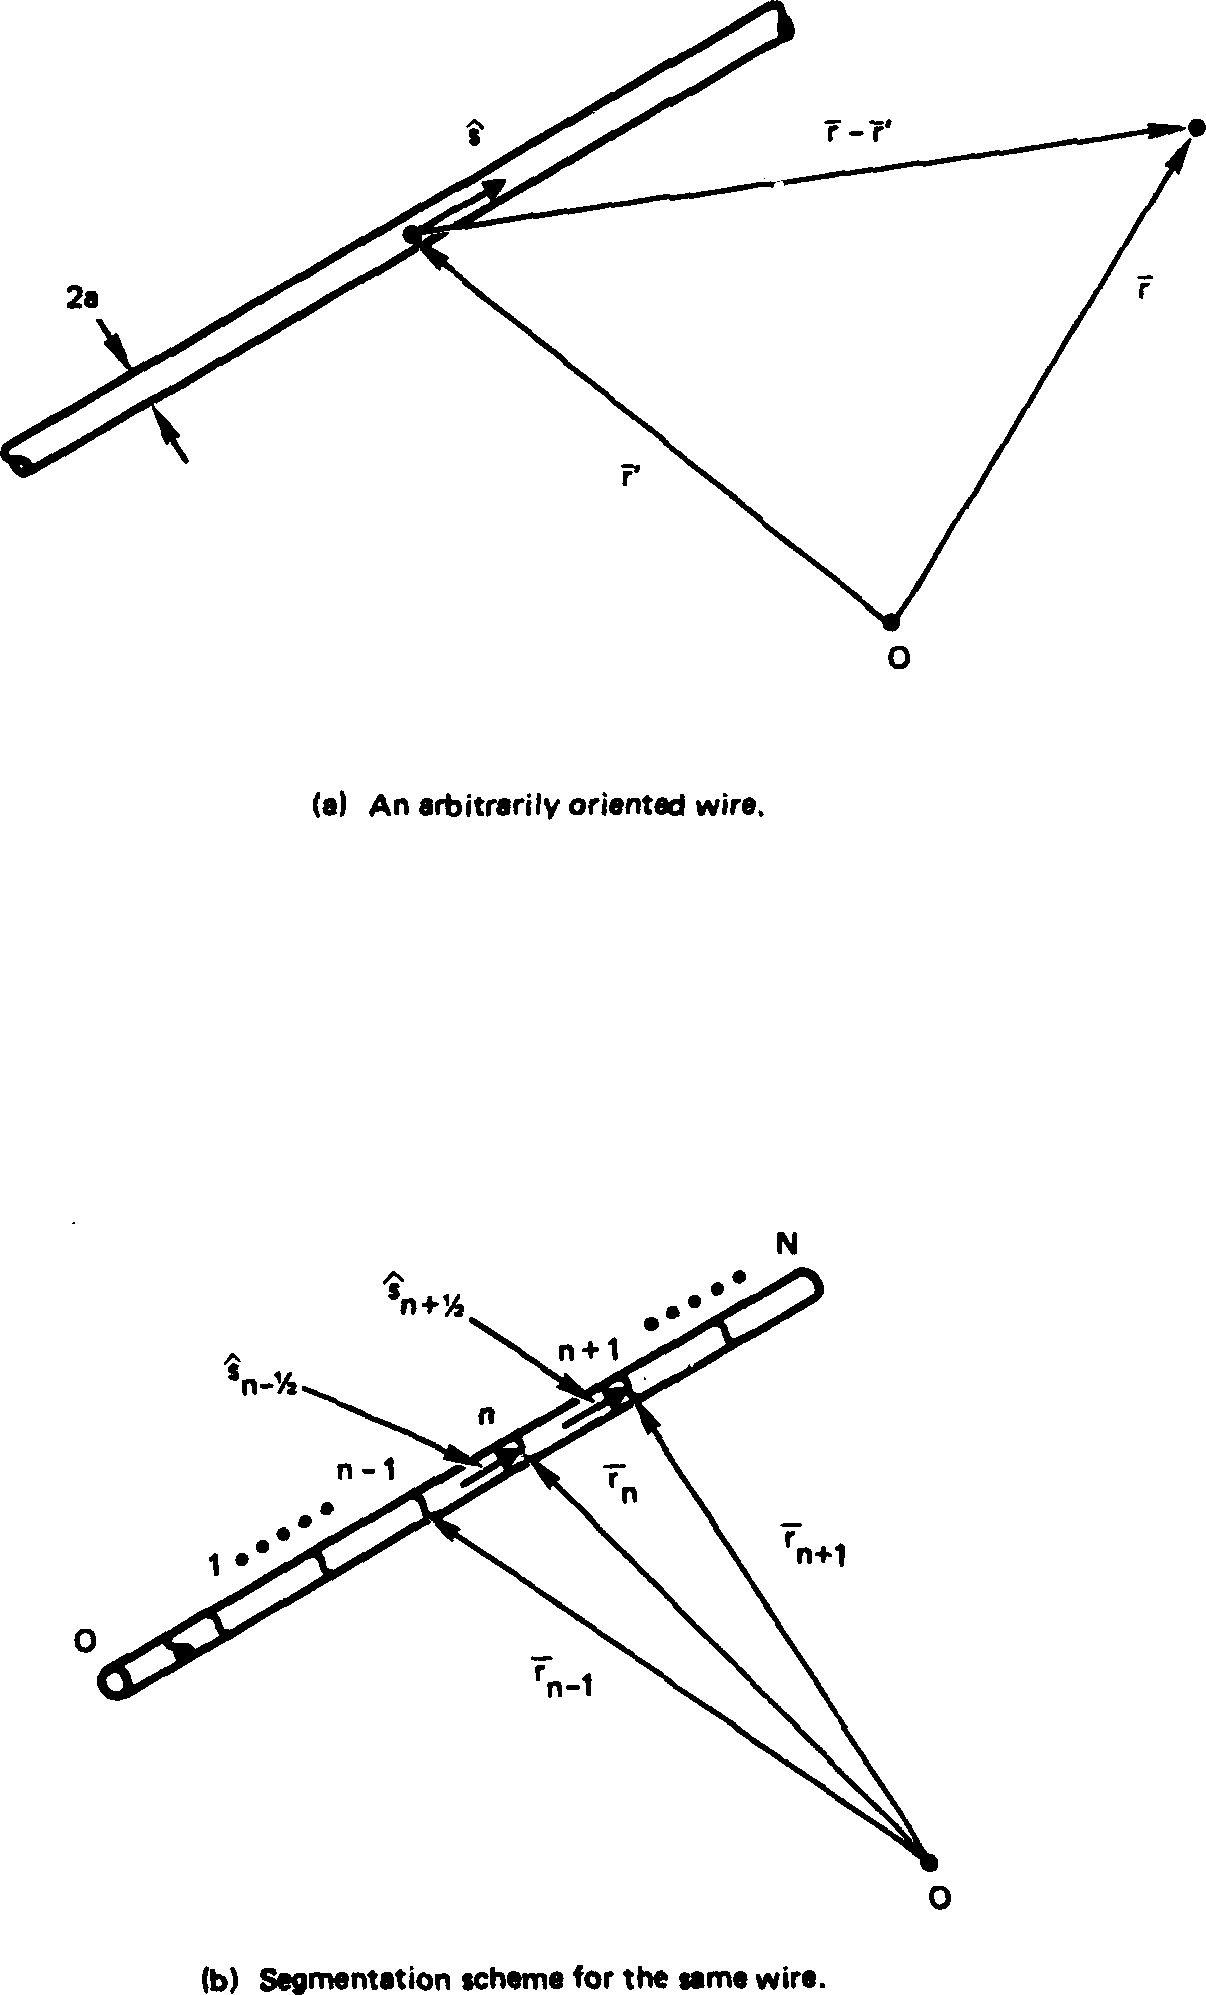
\includegraphics{fig1.eps}}
\caption{Definition of the position vectors with respect to the global
origin O}
\label{fig1}
\end{figure}
\afterpage\clearpage

Figure~\ref{fig1} gives the geometry of a typical, arbitrarily oriented
wire. Assume that the wire is straight, even though the theory applies
equally to bent configurations. The same wire is also shown broken into
segments or subsections.

In equations \eqref{eq1}, \eqref{eq2}, and \eqref{eq3} below, the vector and
scalar potentials are given by

\begin{equation}
\vect{A} = \frac{\mu}{4\pi} \int_c I(s)\hat{s}(s)k(s-s^\prime)\dd{s}
\label{eq1}
\end{equation}

\begin{equation}
\Phi = \frac{1}{4\pi\varepsilon} \int_c q(s)k(s-s^\prime)\dd{s}
\label{eq2}
\end{equation}

where
\[ k(s-s\prime) = \frac{1}{2\pi}\int_{-\pi}^{\pi} \frac{e^{-jkr}}{r}\dd{\phi}
\]

\[ r = \left((s-s^\prime)^2 + 4a^2\sin^2\frac{\phi}{2}\right)^{\frac{1}{2}}
\]

and the linear charge density (via the continuity equation) is
\begin{equation}
q(s) = \frac{-1}{j\omega}\frac{\dd{I}}{\dd{s}}
\label{eq3}
\end{equation}

The kernel $k$ becomes the ``exact kernel'' when
$\vect{r}\rightarrow\vect{r^\prime}$ on $c$, but can be accurately
replaced by the ``reduced kernel,''
$k_0 = e^{-jkr}/r$, $r=\left(|\vect{r} - \vect{r}^\prime|^2+a^2\right)^{1/2}$
for $|\vect{r}-\vect{r^\prime}| \gg a$.

The integral equation relating the incident field, $\Einc$, and the
vector and scalar potentials is

\begin{equation}
-\Einc\cdot\hat{s}=
-j\omega\vect{A}\cdot\hat{s}-\hat{s}\cdot\nabla\Phi
\quad .
\label{eq4}
\end{equation}

Equation \eqref{eq4}, above, is solved in MININEC by using the following
procedure.

The wires are divided into equal segments, and, as shown in
Figure~\ref{fig1}, the vectors $\vect{r}_n, n=0, 1, \ldots N+1$ are
defined, with respect to the global coordinate origin, $0$. The unit
vectors parallel to the wire axis for each segment shown are defined as

\begin{equation}
\hat{s}_{n+1/2} = \frac{\vect{r}_{n+1}
- \vect{r}_n}{|\vect{r}_{n+1}-\vect{r}_n|}
\quad .
\label{eq5}
\end{equation}

Pulse testing and pulse expansion functions used in MININEC are defined as
\begin{equation}
P_n(s) = \left\{
\begin{array}{ll}
1, & s_{n-1/2} < s < s_{n+1/2} \\
0, & \mathrm{otherwise}        \\
\end{array}\right.
\label{eq6}
\end{equation}

\noindent where the points $s_{n\pm1/2}$ designate segment midpoints,

\begin{equation}
s_{n+1/2} = \frac{s_{n+1} + s_n}{2}
\label{eq7}
\end{equation}

\noindent or in terms of the global coordinates,

\begin{equation}
\vect{r}_{n+1/2} = \frac{\vect{r}_{n+1} + \vect{r}_n}{2}
\quad.
\label{eq8}
\end{equation}

It is assumed that the components of the vectors $\Einc$
and $\vect{A}$ in equation \eqref{eq4} are sufficiently smooth over each
segment that their respective values on each segment may be replaced by
those taken at the point $s_m$. The pulse functions of \eqref{eq6} are
then used as testing functions on \eqref{eq4}, resulting in

\begin{equation}
\begin{aligned}
\Einc(s_m)&\cdot
\left[\left(\frac{s_m-s_{m-1}}{2}\right)\hat{s}_{m-1/2}
+ \left(\frac{s_{m+1} - s_m}{2}\right)\hat{s}_{m+1/2}\right] = \\
j\omega\vect{A}(s_m)&\cdot
\left[\left(\frac{s_m-s_{m-1}}{2}\right)\hat{s}_{m-1/2}
+ \left(\frac{s_{m+1}-s_m}{2}\right)\hat{s}_{m+1/2}\right] + \\
\Phi(s_{m+1/2}) &- \Phi(s_{m-1/2}) \\
\end{aligned}
\label{eq9}
\end{equation}

The vector quantities in brackets are simply
$(\vect{r}_{m+1/2} - \vect{r}_{m-1/2})$,
so \eqref{eq9} can be written as

\begin{equation}
\begin{gathered}
\Einc(s_m)\cdot(\vect{r}_{m+1/2}-\vect{r}_{m-1/2}) = \\
j\omega\vect{A}(s_m)\cdot(\vect{r}_{m+1/2}-\vect{r}_{m-1/2})
+\Phi(s_{m+1/2}) - \Phi(s_{m-1/2})
\quad.
\end{gathered}
\label{eq10}
\end{equation}

The currents are expanded in pulses centered at the junctions of
adjacent segments as illustrated in figure~\ref{fig2}(a). Note that pulses
are omitted from the wire ends. This is equivalent to placing a half
pulse of zero amplitude at each end, thus imposing the boundary
condition for zero current at unattached wire ends. The current
expansion can be written as

\begin{equation}
I(s) = \sum_{n=1}^{N} I_n P_n (s)
\quad.
\label{eq11}
\end{equation}

A difference approximation is applied to equation \eqref{eq3} to compute
the charge. Thus, as shown in Figure~\ref{fig2}(b), the charge can be
represented as pulses displaced from the current pulses by a half pulse
width.

\begin{figure}[htb]
\centerline{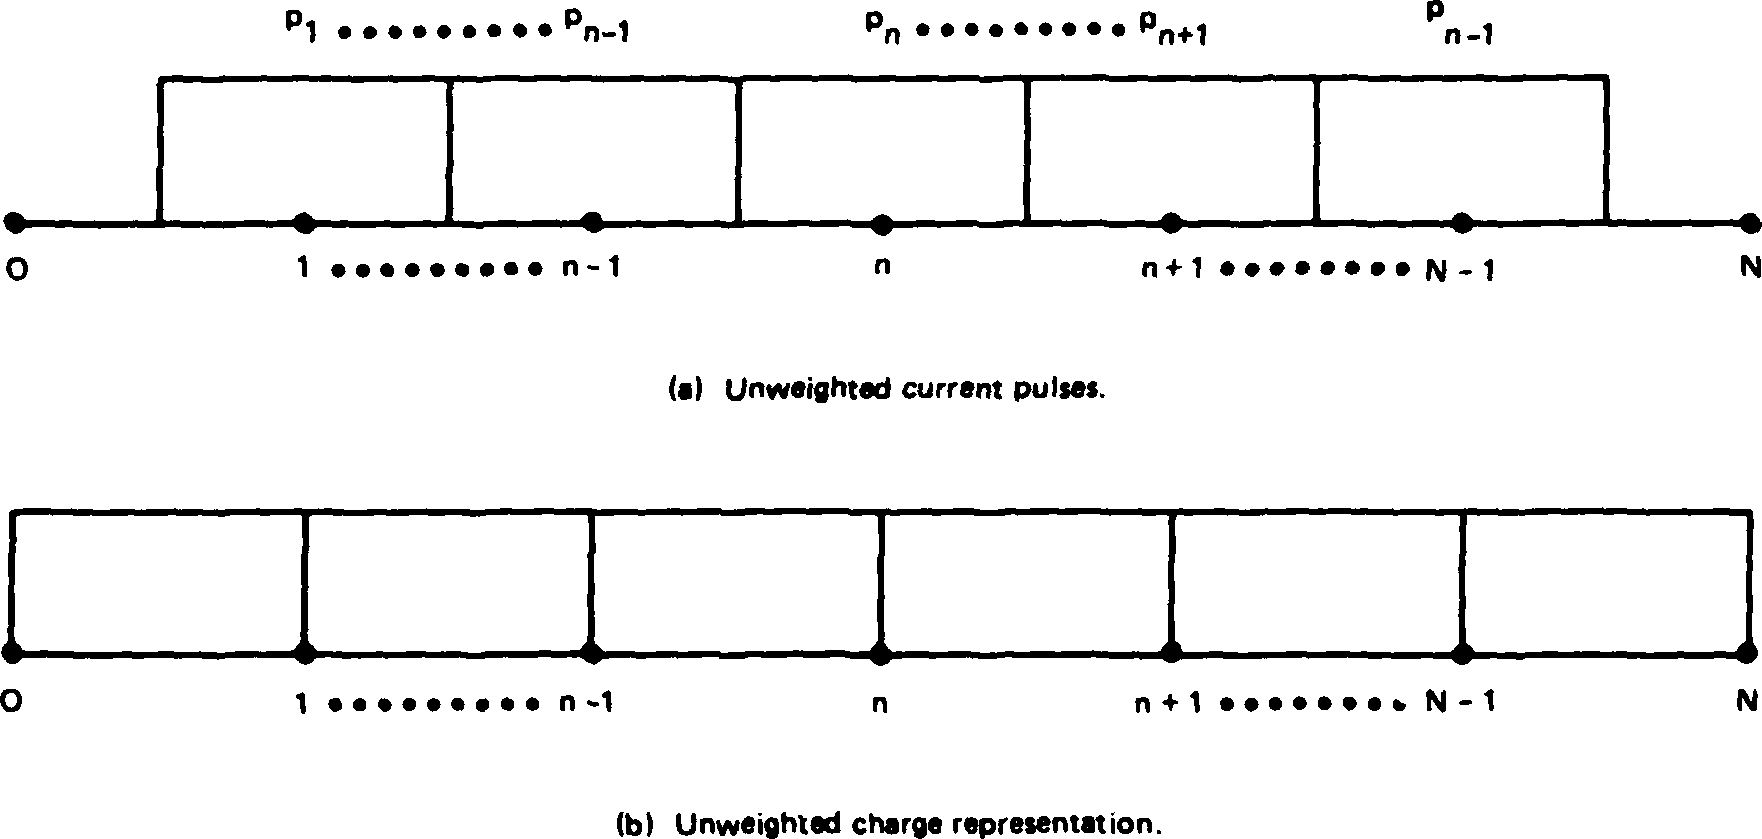
\includegraphics{fig2.eps}}
\caption{Wire segmentation scheme illustrating equally weighted pulses
for current and charge}
\label{fig2}
\end{figure}

Substituting \eqref{eq11} into \eqref{eq10} produces a system of
equations that can be expressed in matrix form. Each matrix element,
$Z_{mn}$, associated with the \mbox{$n$-th} current and the $s_m$ observation
point involves scalar and vector potential terms with integrals of the
form

\begin{equation}
\Phi_{m,u,v} = \int_{s_u}^{s_v} k(s_m - s^\prime)\dd{s^\prime}
\label{eq12}
\end{equation}

\noindent where

\begin{equation}
k(s-s^\prime) = \frac{1}{2\pi}\int_{-\pi}^\pi\frac{e^{-jkr_m}}{r_m}\dd{\phi}
\label{eq13}
\end{equation}

\noindent and

\begin{equation}
r_m = \left((s_m - s^\prime)^2 + 4a^2\sin^2\frac{\phi}{2}\right)^{1/2}
\quad.
\label{eq14}
\end{equation}

Equation \eqref{eq12} does not lend itself to straightforward
integration because of the singularity at $r=0$. The $1/r$ can be
subtracted from the integrand and then added as a separate term to yield

\begin{equation}
k(s-s^\prime) = \frac{1}{2\pi}\int_{-\pi}^\pi \frac{\dd{\phi}}{r_m}
+\frac{1}{2\pi}\int_{-\pi}^\pi\frac{e^{-jkr_m}-1}{r_m}\dd{\phi}
\quad.
\label{eq15}
\end{equation}

The first term of \eqref{eq15} can be rewritten as an elliptic integral
of the first kind \cite{r6}.

\begin{equation}
\frac{\beta}{\pi a}F\left(\frac{\pi}{2}, \beta\right) =
\frac{1}{2\pi}\int_{-\pi}^\pi\frac{\dd{\phi}}{r_m}
\label{eq16}
\end{equation}

\noindent where
\[ \beta=\frac{2a}{\left[(s_m-s^\prime)^2+4a^2\right]^{1/2}}
\]

\noindent $F(\frac{\pi}{2},\beta)$ has an approximation \cite{r6}.

\begin{equation}
\begin{aligned}
F\left(\frac{\pi}{2}, \beta\right) \cong\
& [a_0 + a_1m + a_2m^2 + a_3m^3] \cdot     \\
& [b_0 + b1_m + b_2m^2 + b_3m^3]\ln(1/m)    \\
\end{aligned}
\label{eq17}
\end{equation}

where

\[
m = 1 - \beta^2 = \frac{(s_m - s^\prime)^2}{(s_m - s^\prime)^2 + 4a^2}
\]

\[
\begin{array}{lrl}
a_0 = & 1.38629\ 436112 & b_0 = .5            \\
a_1 = &  .09666\ 344259 & b_1 = .12498\ 59397  \\
a_2 = &  .03590\ 092383 & b_2 = .06880\ 248576 \\
a_3 = &  .03742\ 563713 & b_3 = .03328\ 355346 \\
a_4 = &  .01451\ 196212 & b_4 = .00441\ 787012 \\
\end{array}
\]

Thus

\begin{equation}
\frac{\beta}{\pi a}F\left(\frac{\pi}{2},\beta\right)
\overrightarrow{s\rightarrow s^\prime}
-\frac{1}{\pi a}\ln\left[\frac{|s_m - s^\prime|}{8a}\right]
\label{eq18}
\end{equation}

and this singularity is also subtracted from $k(s_m-s^\prime)$.

\clearpage
Thus

\begin{equation}
\begin{gathered}
k(s_m - s^\prime) = -\frac{1}{\pi a}\ln \left[\frac{|s_m - s^\prime|}{8a}\right]
+\frac{\beta F(\frac{\pi}{2}, \beta)
      + \ln\left[\frac{|s_m - s^\prime|}{8a}\right]}{\pi a}  \\
+ \frac{1}{2\pi}\int_{-\pi}^\pi\frac{e^{-jkr}-1}{r}\dd{\phi} \\
\end{gathered}
\label{eq19}
\end{equation}

This equation is substituted into equation~\eqref{eq12} and written as

\begin{equation}
\int_{s_u}^{s_v} k(s-s^\prime)\dd{s^\prime} = I_1 + I_2 + I_3
\quad.
\label{eq20}
\end{equation}

$I_1$, $I_2$, and $I_3$ are defined as

\begin{equation}
\begin{aligned}
I_1 & = -\frac{1}{\pi a}\int_{s_u}^{s_v}
        \ln\left[\frac{|s-s^\prime|}{8a}\right] \dd{s^\prime}
    & = \left.\frac{8}{\pi} u(1-\ln|u|)\right|_{u_1}^{u_2}
\end{aligned}
\label{eq21}
\end{equation}

where

\[ u_1 = \frac{s_u - s}{8a} \mbox{ and } u_2 = \frac{s_v - s}{8a}
\quad.
\]

\noindent Similarly,

\begin{equation}
I_2 = \int_{s_u}^{s_v}
\frac{\beta F\left(\frac{\pi}{2}, \beta\right)
+ \ln\frac{|s-s^\prime|}{8a}}{\pi a}\dd{s^\prime}
\label{eq22}
\end{equation}

This integral has a well behaved integrand and can be integrated
numerically. The integration is broken up into two integrals over the
ranges $(s_u, s)$ and $(s, s_v)$ for best accuracy. Gaussian quadrature
is used for the numerical integration \cite{r7}. The number
of points used in the integration routine is automatically selected by
consideration of the pulse accuracy required for the source to
observation distance. The final integral is

\begin{equation}
I_3 = \frac{1}{2\pi}\int_{s_u}^{s_v}\int_{-\pi}^\pi\frac{e^{-jkr}-1}{r}\dd{\phi}
\quad.
\label{eq23}
\end{equation}

The integrand is nonsingular and can be integrated numerically. To
obviate the need for double integration, it is convenient to approximate
the integral by replacing $r$ by a reduced kernel approximation of
equation~\eqref{eq14}.

\noindent Thus

\begin{equation}
I_3 = \int_{s_u}^{s_v}\frac{e^{-jkr_a}-1}{r_a}\dd{s^\prime}
\label{eq24}
\end{equation}

\noindent where

\[
r_a = \sqrt{(s_v - s^\prime) + a^2}
\quad.
\]

\noindent The integral can be integrated numerically by the same
procedure as for $I_2$.

Thus, equation~\eqref{eq12} with its singularity problem is evaluated by
adding $I_1$ of equation~\eqref{eq21}, $I_2$ of equation~\eqref{eq22}, and
$I_3$ of equation~\eqref{eq24}.

This approach to evaluate~\eqref{eq12} is accurate for a wide range of
wire radii but breaks down when the radius becomes very small. For very
small radii, equation~\eqref{eq12} may be expressed as a single integral
and evaluated using two terms of a Maclaurin series, after Harrington
\cite{r5}. This approximation for the $\Phi$ terms is:

\begin{equation}
\left.
\begin{array}{ll}
\Phi \approx \frac{1}{2\pi\Delta s}\ln\left(\frac{\Delta s}{a}\right)
-j\frac{k}{4\pi}                   & \mbox{for } m=n          \\
\\
\Phi \approx \frac{e^{-jkr_m}}{4\pi r_m} & \mbox{for } m\ne n \\
\end{array}
\right\}
\quad.
\label{eq25}
\end{equation}

Figure~\ref{fig3} demonstrates the range and validity with and without
the small radius correction. Without the correction, MININEC gives
acceptable answers for wire radii between $10^{-2}$ and $10^{-5}$ wave
lengths. Note that MININEC is within 10\% or better of the data
published by King \cite{r8} \cite{r9}, for radii
between $10^{-3}$ and $10^{-2}$ wave lengths. The small radius
correction provides correct results for radii of $10^{-4}$ wave lengths
or smaller. In MININEC, the switch to the small radius approximations
occurs automatically for radii of $10^{-4}$ and smaller.

By substitution, the matrix equation to be solved is

\begin{equation}
[Z_{mn}] = [I_n] = [V_m]
\label{eq26}
\end{equation}

\noindent where

\begin{equation}
\begin{gathered}\relax
[Z_{mn}] = \left.\frac{-1}{4\pi j\omega\varepsilon}\right[
k^2(\vect{r}_{m+1/2} - \vect{r}_{m-1/2}) \cdot
(\hat{s}_{n+1/2}\Phi_{m,n,n+1/2} + \hat{s}_{n-1/2}\Phi_{m,n-1/2,n}) \\
\left.
-\frac{\Phi_{m+1/2,n,n+1}}{s_{n+1}-s_n}+\frac{\Phi_{m+1/2,n-1,n}}{s_n-s_{n-1}}
+\frac{\Phi_{m+1/2,n,n+1}}{s_{n+1}-s_n}-\frac{\Phi_{m+1/2,n-1,n}}{s_n-s_{n-1}}
\right]\\
\end{gathered}
\label{eq27}
\end{equation}

and
\begin{equation}
V_m = \Einc(s_m)\cdot(\vect{r}_{m+1/2}-\vect{r}_{m-1/2})
\quad.
\label{eq28}
\end{equation}

$[Z_{mn}]$ is a square matrix and $[I_n]$ and $[V_m]$ are column
matrices with $n=1,2,\ldots N$ and $m=1,2,\ldots N$ total unknowns ($N$ is
the total number of current pulses). The extension of these equations to
two or more coupled wires follows the same line of development and will
not be covered here.

The column vector $[V_m]$ represents an applied voltage that
superimposes a constant tangential electric field along the wire for a
distance of one segment length centered coincident with the location of
the current pulses. Hence, for a transmitting antenna, all elements of
$[V_m]$ are set to zero except for the element(s) corresponding to the
segment(s) located at the desired feed point(s). For an incident plane
wave, all elements of $[V_m]$ must be assigned a value depending on the
strength, polarization (or orientation), and angle of incidence of the
plane wave. The applied voltage source (transmit case), however, is the
only ready-made, or programmed, option in MININEC.

As stated above, the $[Z_{mn}]$ matrix in equation~\eqref{eq26} is
filled by the evaluation of an elliptic integral and use of Gaussian
quadrature for numerical integration. The solution of~\eqref{eq26} can
be accomplished by using any one of a number of standard matrix solution
techniques. MININEC(3) uses a triangular decomposition (LU
decomposition) with the Gauss elimination procedure with partial
pivoting \cite{r7}.

\begin{sidewaysfigure}[htb]
\centerline{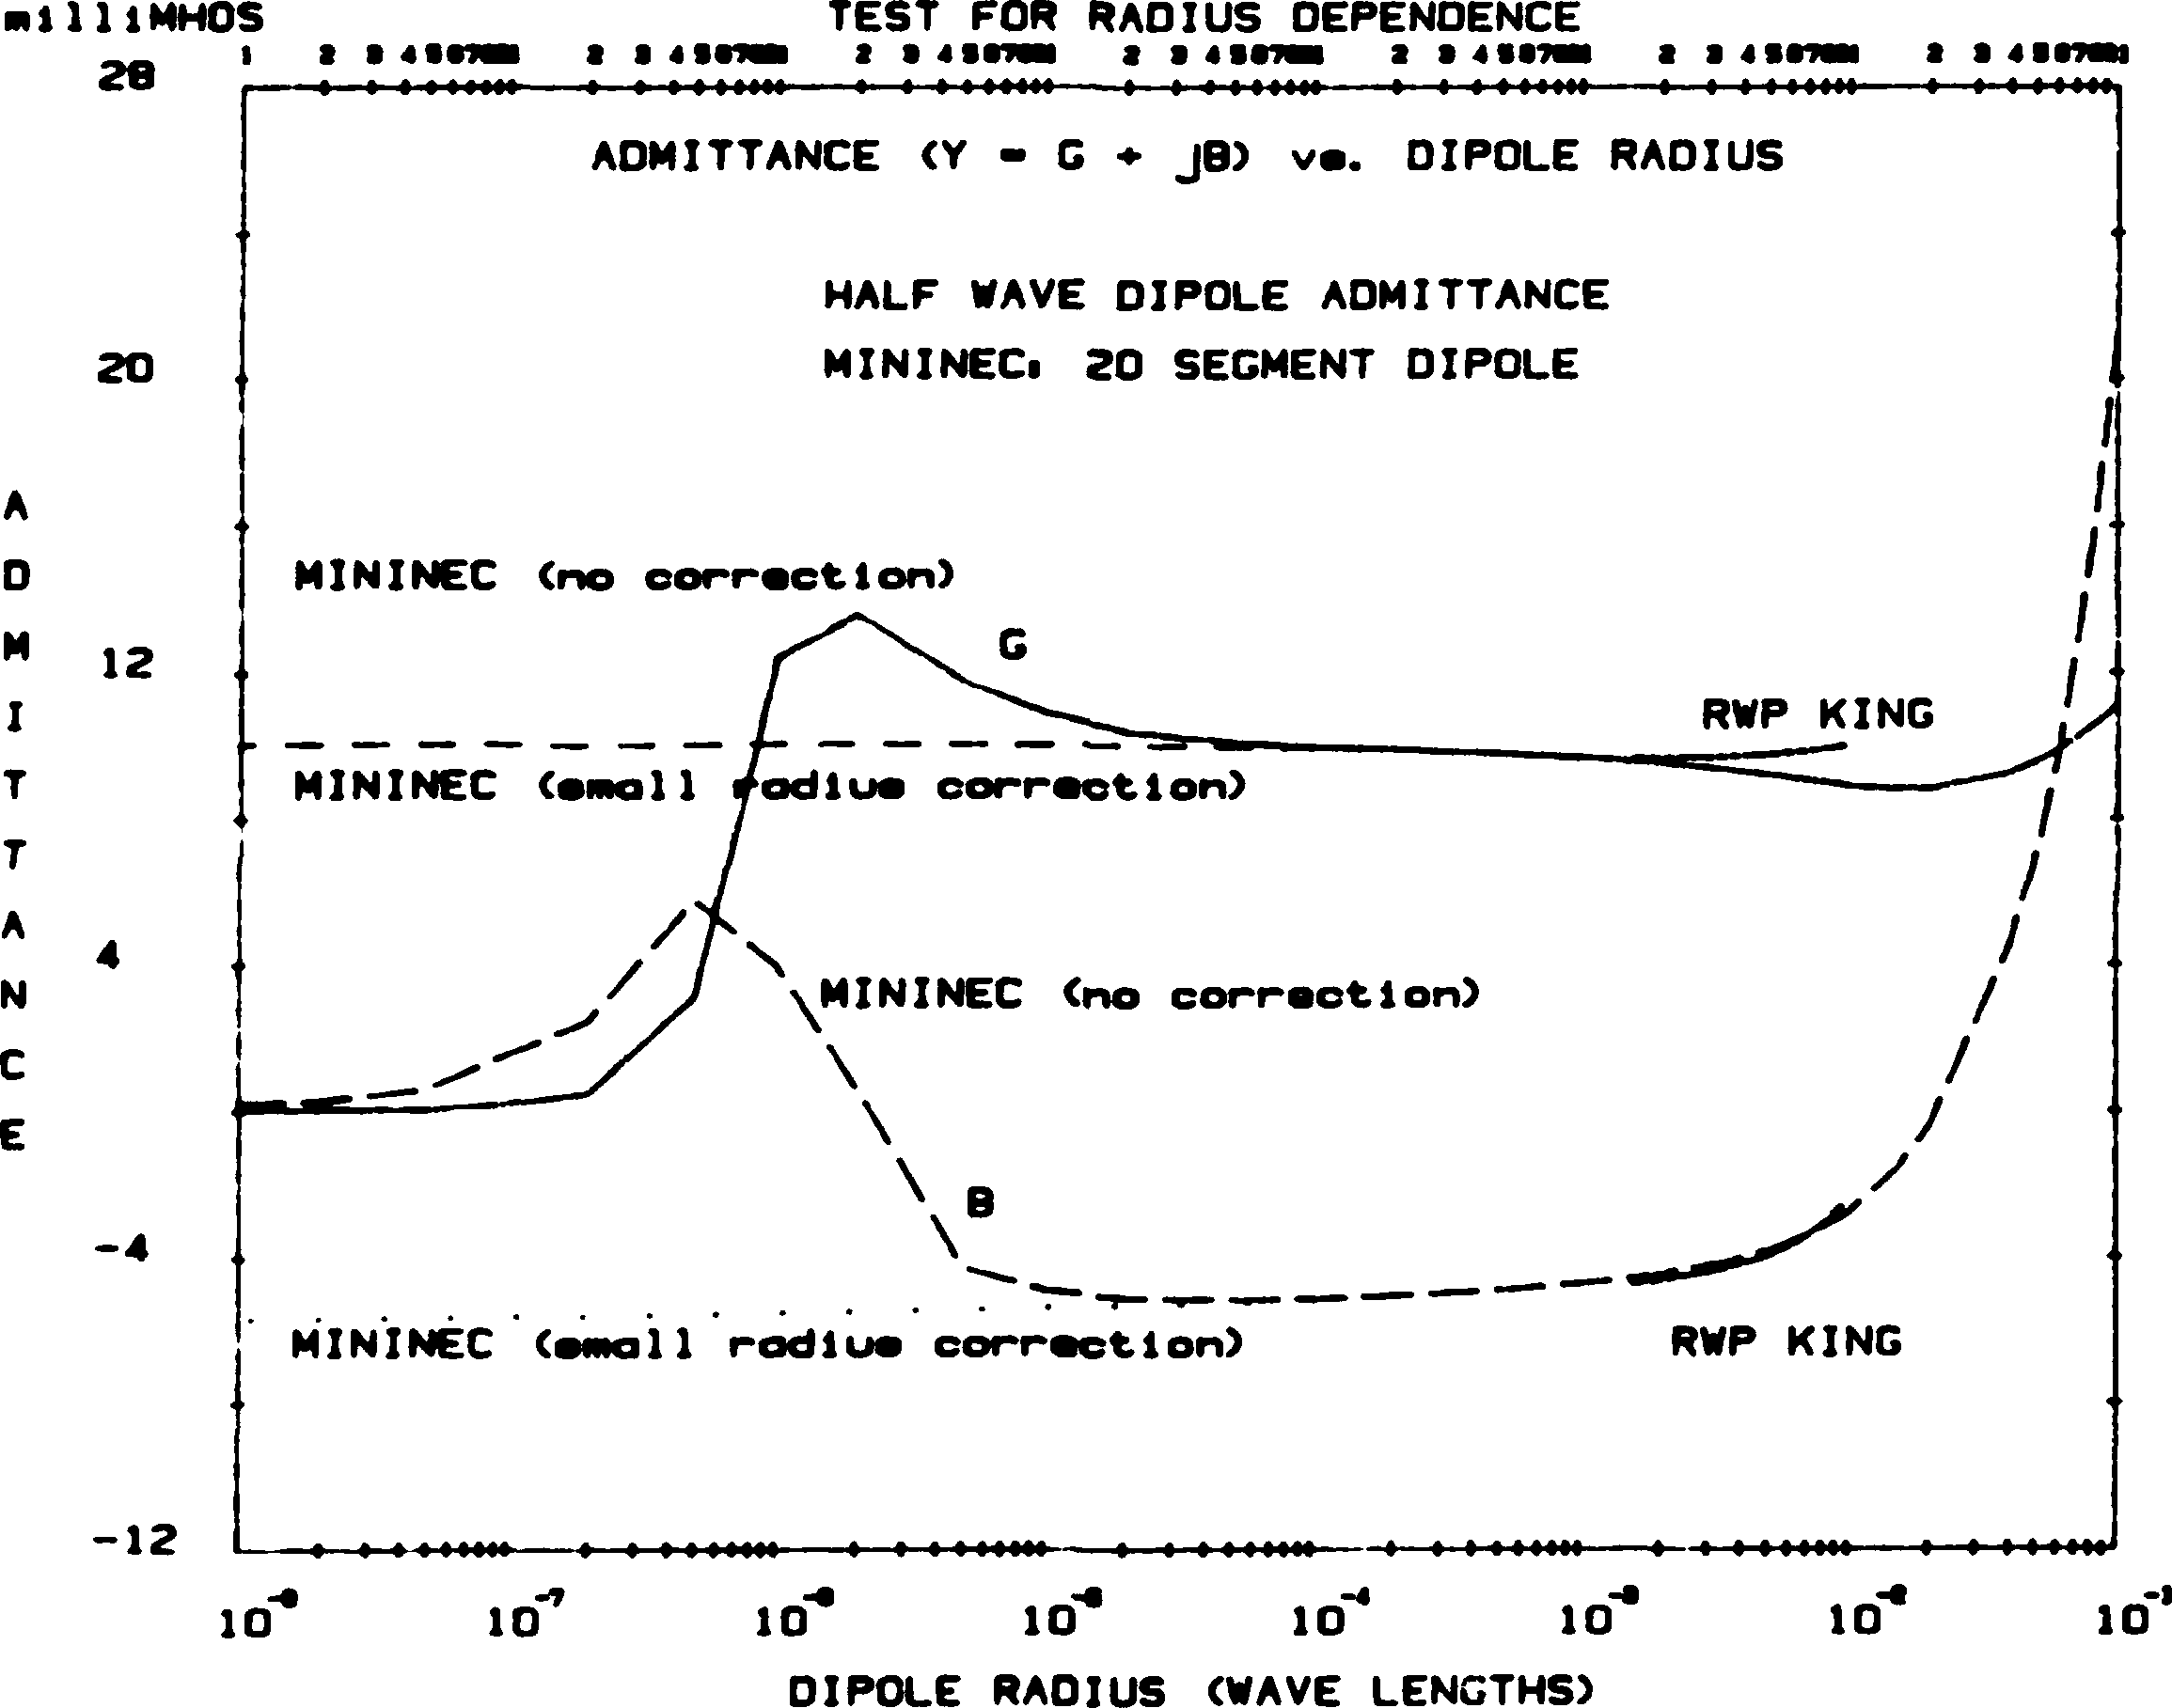
\includegraphics{fig3.eps}}
\caption{Variation of dipole admittance with wire radius for MININEC
with and without the small radius correction. Data from King
\cite{r8}, \cite{r9} is also shown.}
\label{fig3}
\end{sidewaysfigure}
\afterpage\clearpage

\subsection{Wire Junctions}
The theory developed thus far for straight wires is equally applicable
to bent wires. However, for coding simplicity in MININEC, bent wires are
treated in the same way as the junctions of multiple numbers of wires.
That is, a bend in an otherwise straight wire is treated as the junction
between two straight wires.

It has been generally accepted that the currents at junctions of thin
wires conform to Kirchoff's current law \cite{r10}. Rather
than explicitly enforcing this condition in MININEC, an overlapping
segment scheme \cite{r11} is employed at junctions of two or
more wires. A detailed discussion of this approach, including arguments
for validity, appears in both references~\cite{r8} and~\cite{r9}. Only
those aspects essential to the use of MININEC are discussed here.

Consider a wire having no connections at either end. The wire is
subdivided into segments and the current is expanded in pulses centered
at adjacent segment junctions as described above and illustrated in
Figure~\ref{fig4}(a). The end points have no pulses, or alternatively the
end points have half pulses with zero amplitude. A second wire is to be
attached to one end of the first. The second wire is subdivided into
segments with pulses for currents located as in the first case. However,
a full pulse is located at the attachment end, with half the pulse
extending onto wire two, and half onto wire one, as illustrated in
Figure~\ref{fig4}(b). The half on wire one assumes the dimensions (length
and radius) of the half segment on wire one, while the half on wire two
assumes the dimensions appropriate to wire two. Wire two overlaps onto
wire one with a full pulse centered at the junction end. Note that the
free end of the wire has a zero half pulse. A third wire may be assumed
to also overlap onto wire one, as illustrated in Figure~\ref{fig4}(c). It can
be shown (see \cite{r8} and \cite{r9}) that for a junction of
$N$ wires, only $N-1$ overlapping pulses are required to satisfy
Kirchoff's current law. Alternatively, wire three could have overlapped
onto wire two (not illustrated here).

The convention in MININEC(3) is that the overlap occurs onto the
earliest wire specified at a given junction. It is assumed that a wire
can overlap onto another wire, provided that another wire was previously
specified. It cannot overlap onto a wire not yet specified. Either end
of a wire may overlap onto either end of another wire. All that is
required to impose the continuity conditions at the junction is that
there be $N-1$ overlaps for a junction of $N$ wires.

Current reference directions are assumed to be based on the order in
which the coordinates of a wire are specified. A positive wire current
is from the end first specified, end one, towards the other end, end
two. By use of Kirchoff's current law and the current reference
direction, the currents at the junction can be found. For example,
suppose the wires in Figure~\ref{fig4}(c) are all specified from left to
right. Let the pulse amplitudes for the first pulse on wires two and
three be $I_2$ and $I_3$, respectively. Then the currents out of the
junction into wires two and three are the complex amplitudes of the
first pulses, the overlapping pulses, on wires two and three,
respectively. Hence, the current on wire one into the junction is the
sum of these currents; i.e., $I_1=I_2+I_3$.

\begin{figure}[htb]
\centerline{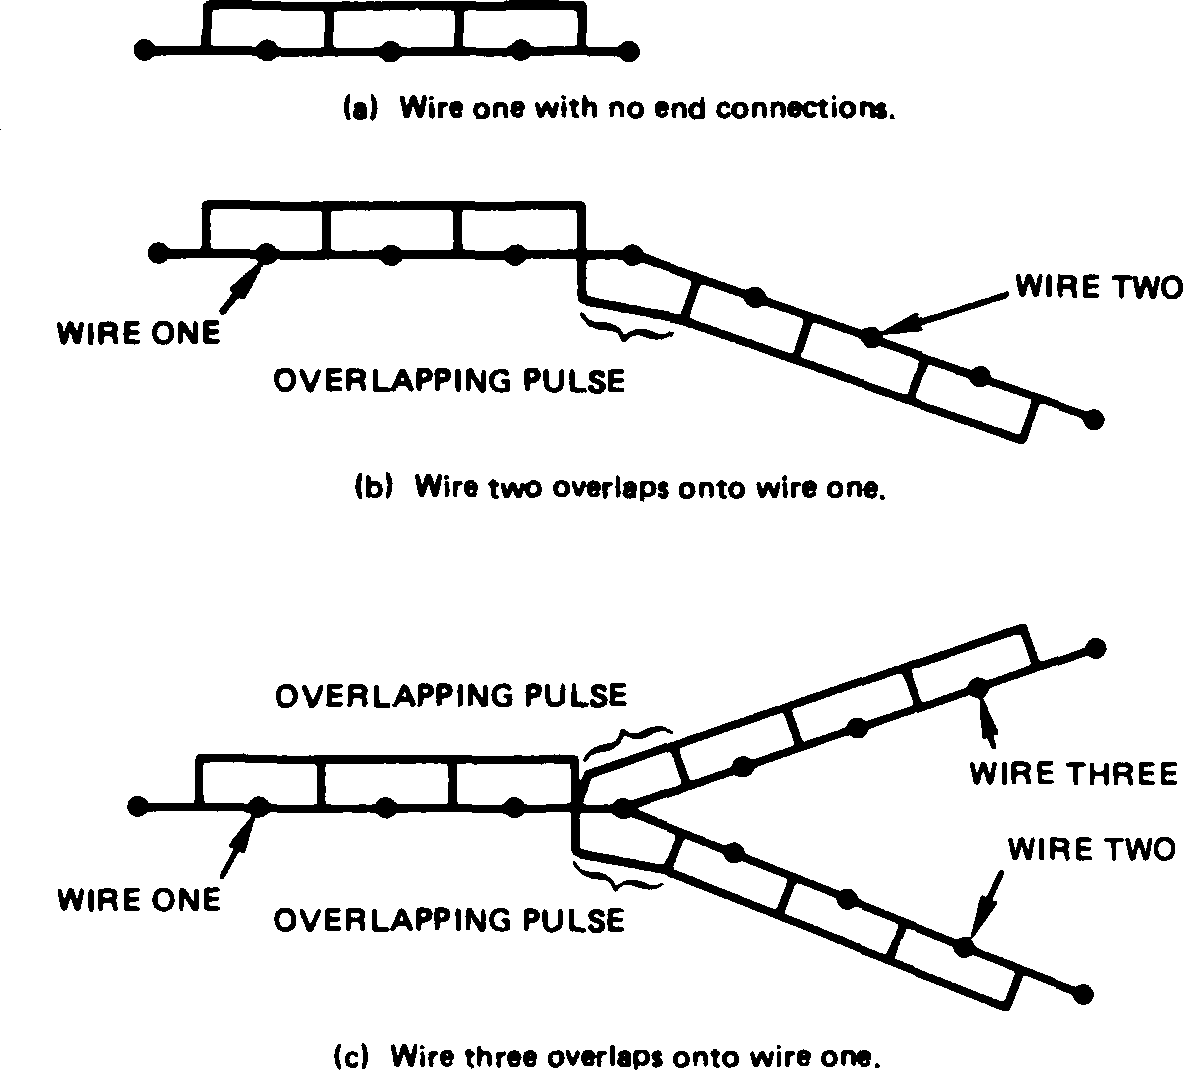
\includegraphics{fig4.eps}}
\caption{Illustration of the overlap scheme used at multiple wire junctions}
\label{fig4}
\end{figure}

MININEC(3) automatically determines, during geometry input, whether
there is a connection on either end of a wire, and if so, to which wire
and wire end it is connected. After solving for the current pulse
amplitudes, MININEC(3) then computes the junction currents, if any, for
each wire end. The final display indicates free ends by the letter
\verb+E+ (for free end) and junction ends by the letter \verb+J+. The
geometry and currents are displayed wire by wire.

\subsection{The Ground Plane}
\label{sec-groundplane}

The method of images is used in MININEC to solve for currents in wires
located over a perfectly conducting ground plane.

Consider a wire structure represented by $N$ segments. In the presence
of a perfectly conducting ground plane, by image theory, the structure
and ground plane may be replaced by the original structure and its
image. Hence, there are now $2N$ segments and $2N$ unknowns to be
determined. Equation~\eqref{eq26} can be written as

\begin{equation}
\left[
\begin{array}{l}
V_1    \\
\vdots \\
V_N    \\
\vdots \\
V_{2N} \\
\end{array}
\right]
=
\left[
\begin{array}{lllll}
Z_{11}   & \cdots & Z_{1N} & \cdots & Z_{1,2N}  \\
\vdots   &        &\vdots  &        & \vdots    \\
Z_{N1}   & \cdots & Z_{NN} & \cdots & Z_{N,2N}  \\
\vdots   &        &\vdots  &        & \vdots    \\
Z_{2N,1} & \cdots &\cdot   & \cdots & Z_{2N,2N} \\
\end{array}
\right]
=
\left[
\begin{array}{l}
I_1    \\
\vdots \\
I_N    \\
\vdots \\
I_{2N}    \\
\end{array}
\right]
\label{eq29}
\end{equation}

The image current, $I_{N+1}\cdots I_{2N}$, are equal to the currents on
the original structure, $I_1\cdots I_N$, so that $I_n = I_{2N-n+1}$. Half
the equations represented in~\eqref{eq29} contain redundant information
and may be discarded. It may be reduced to a square matrix again by
adding appropriate columns; i.e., by using the current identity.
Hence~\eqref{eq29} becomes

\begin{equation}
V=[Z^\prime_{ij}]I
\label{eq30}
\end{equation}

\noindent where $Z^\prime_{ij} = Z_{ij} + Z_{i\ 2N-j+1}$.

For a wire attached to ground, a current pulse is automatically added to
the wire end point connected to ground so that current continuity with
its image is observed; i.e., a non-zero half pulse is placed on both the
wire end and its image. The voltage in equation~\eqref{eq30} is divided
by two in this case. Either end of a wire may be attached to ground.

\subsection{Lumped Parameter Loading}
The wire structures discussed so far consist of perfectly conducting
wires. If an impedance due to a fixed load, $Z_L = R + jX$, is added to
the structure so that its location coincides with that of one or more of
the non-zero-current pulse functions (i.e., a lumped load is placed on
the wire at the junction of two segments), then the load introduces an
additional voltage (a voltage drop) equal to the product of the current
pulse magnitude and $Z_L$. Hence, equation~\eqref{eq26} becomes

\begin{equation}
[Z^\prime_{mn}][I_n]=[V_m]
\label{eq31}
\end{equation}

where $Z^\prime_{mn}=Z_{mn}$ for $m\ne n$ and $Z^\prime_{mn}=Z_{mn}+Z_L$
for $m=n$. Hence, a specified impedance represented as the sum of a
resistance and a reactance, and located on a wire coincident with a
current pulse is simply added to the diagonal impedance element or
self-term corresponding to that pulse. A distributed impedance such as
wire conductivity can be treated in the same way by use of an
equivalent, lumped-circuit, element-impedance relationship.

\subsection{Near Fields}
The electric near fields and the magnetic near fields can be determined
from the current distribution obtained in the solution of
equation~\eqref{eq26}.

The near electric fields are computed by the method described by
A.~T. Adams, et al., \cite{r12}. Using MININEC, the current
on the wire structure is approximated using the computed current pulses.
To determine the electric field at a given point in the near field, a
small, virtual thin-wire dipole is placed at the point with its axis
parallel to the appropriate vector component. The open-circuit voltage
at the near field point can be calculated from the knowledge of the
current distribution over the wire structure and the mutual impedance
between the wire structure and the virtual dipole. In other words,

\begin{equation}
V_d = \sum_{i=1}^{N}Z_{di}I_i \quad.
\label{eq32}
\end{equation}

The virtual dipole is open-circuited. $V_d$ is the open-circuit voltage.
$I_i$ are the MININEC computed current pulses of the wire structure.
$Z_{di}$ are the mutual impedances between the wire structure and the
virtual dipole. The mutual impedances are calculated using the MININEC
method of equation~\eqref{eq27}. The electric field strength along the
direction of the virtual dipole is given by

\begin{equation}
E_d = -\frac{V_d}{\mbox{length of dipole}}\quad.
\label{eq33}
\end{equation}

This equation is evaluated once for each electric field vector component
in the $x$, $y$ and $z$ directions at the near field point of interest.
In MININEC, a virtual dipole of length .001 wave length is used.

MININEC calculates the three vector components $E_x$, $E_y$ and $E_z$,
as real and imaginary terms, from which the magnitude and phase are
determined. The average value is determined by

\begin{equation}
\ave{E} = \left[\frac{1}{2}(E_x^2+E_y^2+E_z^2)\right]^{1/2}
\label{eq34}
\end{equation}

\noindent which is a conservative estimate of the maximum value. The maximum or
peak electric field is determined by the method described by Adams and
Mendelovicz \cite{r13}. The peak electric field is

\begin{equation}
\peak{E} = \left[\frac{1}{2}(E_x^2+E_y^2+E_z^2)
                +\frac{1}{2}(A^2+B^2)^{1/2} \right]^{1/2}
\label{eq35}
\end{equation}

\noindent where
\[ A = E_x^2\cos 2\theta_x + E_y^2\cos 2\theta_y + E_z^2\cos 2\theta_z
\]
\[ B = E_x^2\sin 2\theta_x + E_y^2\sin 2\theta_y + E_z^2\sin 2\theta_z
\]

\noindent and where $\theta_x$, $\theta_y$, and $\theta_z$ are the phase
angles for the corresponding field component.

The near magnetic fields are computed by a comparable method. As is the
case for electric near fields, the currents on the wires are
approximated by the current pulses of the MININEC solution. A virtual,
thin-wire dipole is placed at the near field point with its axis
parallel to the appropriate vector component. The near magnetic field is
then calculated using the MININEC current distribution and the
difference between the appropriate components of the vector potential.

The vector potential is generally defined such that

\begin{equation}
\Hplus = \frac{1}{\mu}\nabla X\Aplus
\label{eq36}
\end{equation}

\noindent expressed in rectangular coordinates, becomes

\begin{equation}
\mu\Hplus =
\left(\frac{\partial A_z}{\partial y} - \frac{\partial A_y}{\partial z}\right)
\hat{i} +
\left(\frac{\partial A_x}{\partial z} - \frac{\partial A_z}{\partial x}\right)
\hat{j}+
\left(\frac{\partial A_y}{\partial x} - \frac{\partial A_x}{\partial y}\right)
\hat{k}
\label{eq37}
\end{equation}

whre $\hat{i}$, $\hat{j}$, $\hat{k}$ are the unit vectors parallel to
the $x$, $y$, $z$ coordinate axis, respectively. And where $A_x$, $A_y$,
$A_z$ are the corresponding components of the vector potential evaluated
at the location of the virtual dipole (i.e., the near field point). If
the virtual dipoles are electrically short enough so that the fields
vary continuously and smoothly over the dipole length, the partial
derivatives of equation~\eqref{eq37} can be replaced by differences:

\begin{equation}
\mu\Hplus =
\left(\frac{\Delta A_z}{\Delta y} - \frac{\Delta A_y}{\Delta z}\right)
\hat{i} +
\left(\frac{\Delta A_x}{\Delta z} - \frac{\Delta A_z}{\Delta x}\right)
\hat{j}+
\left(\frac{\Delta A_y}{\Delta x} - \frac{\Delta A_x}{\Delta y}\right)
\hat{k}
\label{eq38}
\end{equation}

such that, for example, $\Delta A_z/\Delta_y$ is the change in the
Z-component of the vector potential along a y-directed virtual dipole of
length $\Delta y$, located at the near field point, etc. In MININEC, the
virtual dipole length is .001 wave length for both the near electric and
near magnetic field calculations.

MININEC calculates the three vector components, $H_x$, $H_y$ and $H_z$
as real and imaginary terms, from which the magnitude and phase are
determined. The average and peak values of the magnetic near fields are
found in the same way as they are for the electric near fields. Thus,

\begin{equation}
\ave{H} = \left[\frac{1}{2}(H_x^2 + H_y^2 + H_z^2)\right]^{1/2}
\label{eq39}
\end{equation}

\noindent and

\begin{equation}
\peak{H} = \left[\frac{1}{2}(H_x^2 + H_y^2 + H_z^2)
                +\frac{1}{2}(A^2 + B^2)^{1/2} \right]^{1/2}
\label{eq40}
\end{equation}

\noindent where

\[ A = H_x^2\cos 2\theta_x + H_y^2\cos2\theta_y + H_z^2\cos2\theta_z
\]
\[ B = H_x^2\sin 2\theta_x + H_y^2\sin2\theta_y + H_z^2\sin2\theta_z
\]

\noindent and $\theta_i$ are the corresponding phase angles.

Both the electric and magnetic near fields can be scaled for any desired
radiated power from the wire structure since the near fields are
directly proportional to the square root of the power radiated.

\subsection{Far Zone Radiation Patterns}
Once the induced currents on the wires have been determined from
equation~\eqref{eq25}, the radiated electric fields are computed by

\begin{equation}
\vect{E}(\vect{r}_0) = \int_L\frac{jk\eta}{4\pi} + \frac{e^{-jkr_0}}{r_0}
+\left[\hat{k} + \vect{I}(s)\hat{k}-\vect{I}(s)\right]
e^{i\vect{K}\cdot\vect{r}}\dd{s}
\label{eq41}
\end{equation}

\noindent where $\vect{r}_0$ is the position vector at the observation point,
$\bar{k} = \vect{r}_0 / |\vect{r}_0|$, and
$\vect{K} = k\hat{k} = \frac{2\pi}{\lambda}\hat{k}$. The integral is
evaluated in closed form over each straight wire segment for each
current pulse and is reduced to the summation over the wire segments.
The fields are then evaluated as real and imaginary parts of the
$\theta$ and $\phi$ components at a specified radial distance. If the
radial distance is zero, the factor $e^{-jkr_0}/r_0$ defaults to unity.

The power gain in MININEC is evaluated with the $e^{-jkr_0} / r_0$
factor set to one in an approach similar to that in NEC
\cite{r4}. The power gain in a given direction
$(\theta, \phi)$ in spherical coordinates is

\begin{equation}
G = 10 \log\left(\frac{4\pi P(\theta,\phi)}{\Pin}\right)
\label{eq42}
\end{equation}

\noindent where $P(\theta,\phi)$ is the power radiated per unit steradian in the
direction $(\theta, \phi)$ and $\Pin$ is the total input power to the
antenna. Note that directive gain could be obtained by replacing
$\Pin$ by the total power radiated. This step is not done in MININEC.
$\Pin$ is calculated from the applied voltages and the corresponding
feed point currents as

\begin{equation}
\Pin = \sum_{i=1}^{N}(1/2) \RE(V_n I_n^*)
\label{eq43}
\end{equation}

\noindent where $I_n^*$ denotes complex conjugate and $n$ is the number of
sources. $P(\theta,\phi)$ is determined from

\begin{equation}
P(\theta,\phi) = \frac{1}{2} r_0^2 \RE[\vect{E}\times\vect{H}]
= \frac{r_0^2}{2\eta}\vect{E}\cdot\vect{E}^*
\label{eq44}
\end{equation}

\noindent
where $r_0$ is the magnitude of the position vector $\vect{r}_0$ in the
$(\theta,\phi)$ direction. In MININEC, the gains are calculated for the
individual orthogonal components of the field determined from
equation~\eqref{eq41}. The power gain thus obtained from \eqref{eq42} is
in dB above the gain of an isotropic antenna (sometimes denoted as dBi).

MININEC includes an option to correct the far fields and gain for the
effects of real ground using a Fresnel reflection coefficient. The
method is similar to the far field corrections used in NEC
\cite{r4}, but is not limited to one or two mediums. The
surface of the ground is divided into a finite number of zones with a
constant conductivity and dielectric constant in each zone, i.e., a
constant surface impedance for each zone. The zones are defined by
circular boundaries concentric about the origin or linear boundaries
parallel to the y-axis and spaced along the positive x-axis. Thus, in
the latter case, the ground surface is divided into ``strips'' at user
defined x-axis intercepts. In the former case, the ground surface is
divided into concentric rings at user specified radii. In this case, the
first ring, or zone, may include a radial wire ground screen. For both
circular and linear zone grounds, each zone may have a different surface
impedance and each zone may have a different height (Z-coordinate)
relative to the first zone. In MININEC, the number of zones is limited
by an array dimension and is currently set to 5.

In the Fresnel reflection coefficient method, the far field is obtained
by summing the contributions of a direct ray and a reflected ray from
each current pulse. The field, due to the reflected ray, is modified by
the Fresnel plane wave reflection coefficient, which depends on the
ground surface impedance at the bounce point, or specular point, and the
angle of incidence.

The Fresnel reflection coefficients have not been applied to the MININEC
current calculation. When a real ground is specified, the currents are
calculated by using the perfectly conducting image theory (described in
section~\ref{sec-groundplane}). The real ground corrections are applied
to the far field calculations only. This compromise is designed to keep
MININEC relatively compact and provide accurate results whenever the
ground directly beneath the antenna is a good conductor.

Following along the lines of the development given by Burke and Poggio
\cite{r4}, a wave incident upon a finite ground (i.e., a
real ground) yields a reflected field, $\vect{E}_r$, given by

\begin{equation}
\vect{E}_R = R_H\left[(\vect{E}_I\cdot\hat{P})\hat{P}\right]
           + R_V\left[\vect{E}_I-(\vect{E}_I\cdot\hat{P})\hat{P}\right]
\label{eq45}
\end{equation}

\noindent or

\begin{equation}
\vect{E}_R = R_V\vect{E}_I + (R_H - R_V)(\vect{E}_I\cdot\hat{P})\hat{P}
\label{eq46}
\end{equation}

\noindent where $\hat{P}$ is a unit vector perpendicular to the plane of
incidence. $\vect{E}_I$ is the incident field and $R_V$ and $R_H$ are
the vertical and horizontal reflection coefficients, respectively.

The two terms in square brackets in equation~\eqref{eq44} correspond to
horizontally and vertically polarized waves. The reflected field is
obtained by decomposing the incident field into horizontally and
vertically polarized waves, computing a reflected wave for each, and
recombining the two.

The vertical and horizontal coefficients are

\begin{equation}
R_V = \frac{\cos\theta - z\sqrt{1-z^2\sin^2\theta}}
           {\cos\theta + z\sqrt{1-z^2\sin^2\theta}}
\label{eq47}
\end{equation}

\begin{equation}
R_H = \frac{-\left(z\cos\theta - \sqrt{1-z^2\sin^2\theta}\right)}
           {\cos\theta + z\sqrt{1-z^2\sin^2\theta}}
\label{eq48}
\end{equation}

\noindent where $\theta$ is the angle of incidence and $Z$ is the relative
impedance of the ground surface (relative to the free space impedance).

For a given observation direction $(\theta, \phi)$, the $\hat{P}$ vector
normal to the plane of incidence is

\begin{equation}
\hat{P} = (-\sin\theta, \cos\phi)
\label{eq49}
\end{equation}

\noindent as may be seen in Figure~\ref{fig5}(c). In addition, the $\hat{r}_0$
vector, pointing in the observation direction, is

\begin{equation}
\hat{r}_0 = (\sin\theta\cos\phi, sin\theta\sin\phi, \cos\theta)
\label{eq50}
\end{equation}

\begin{figure}[htb]
\centerline{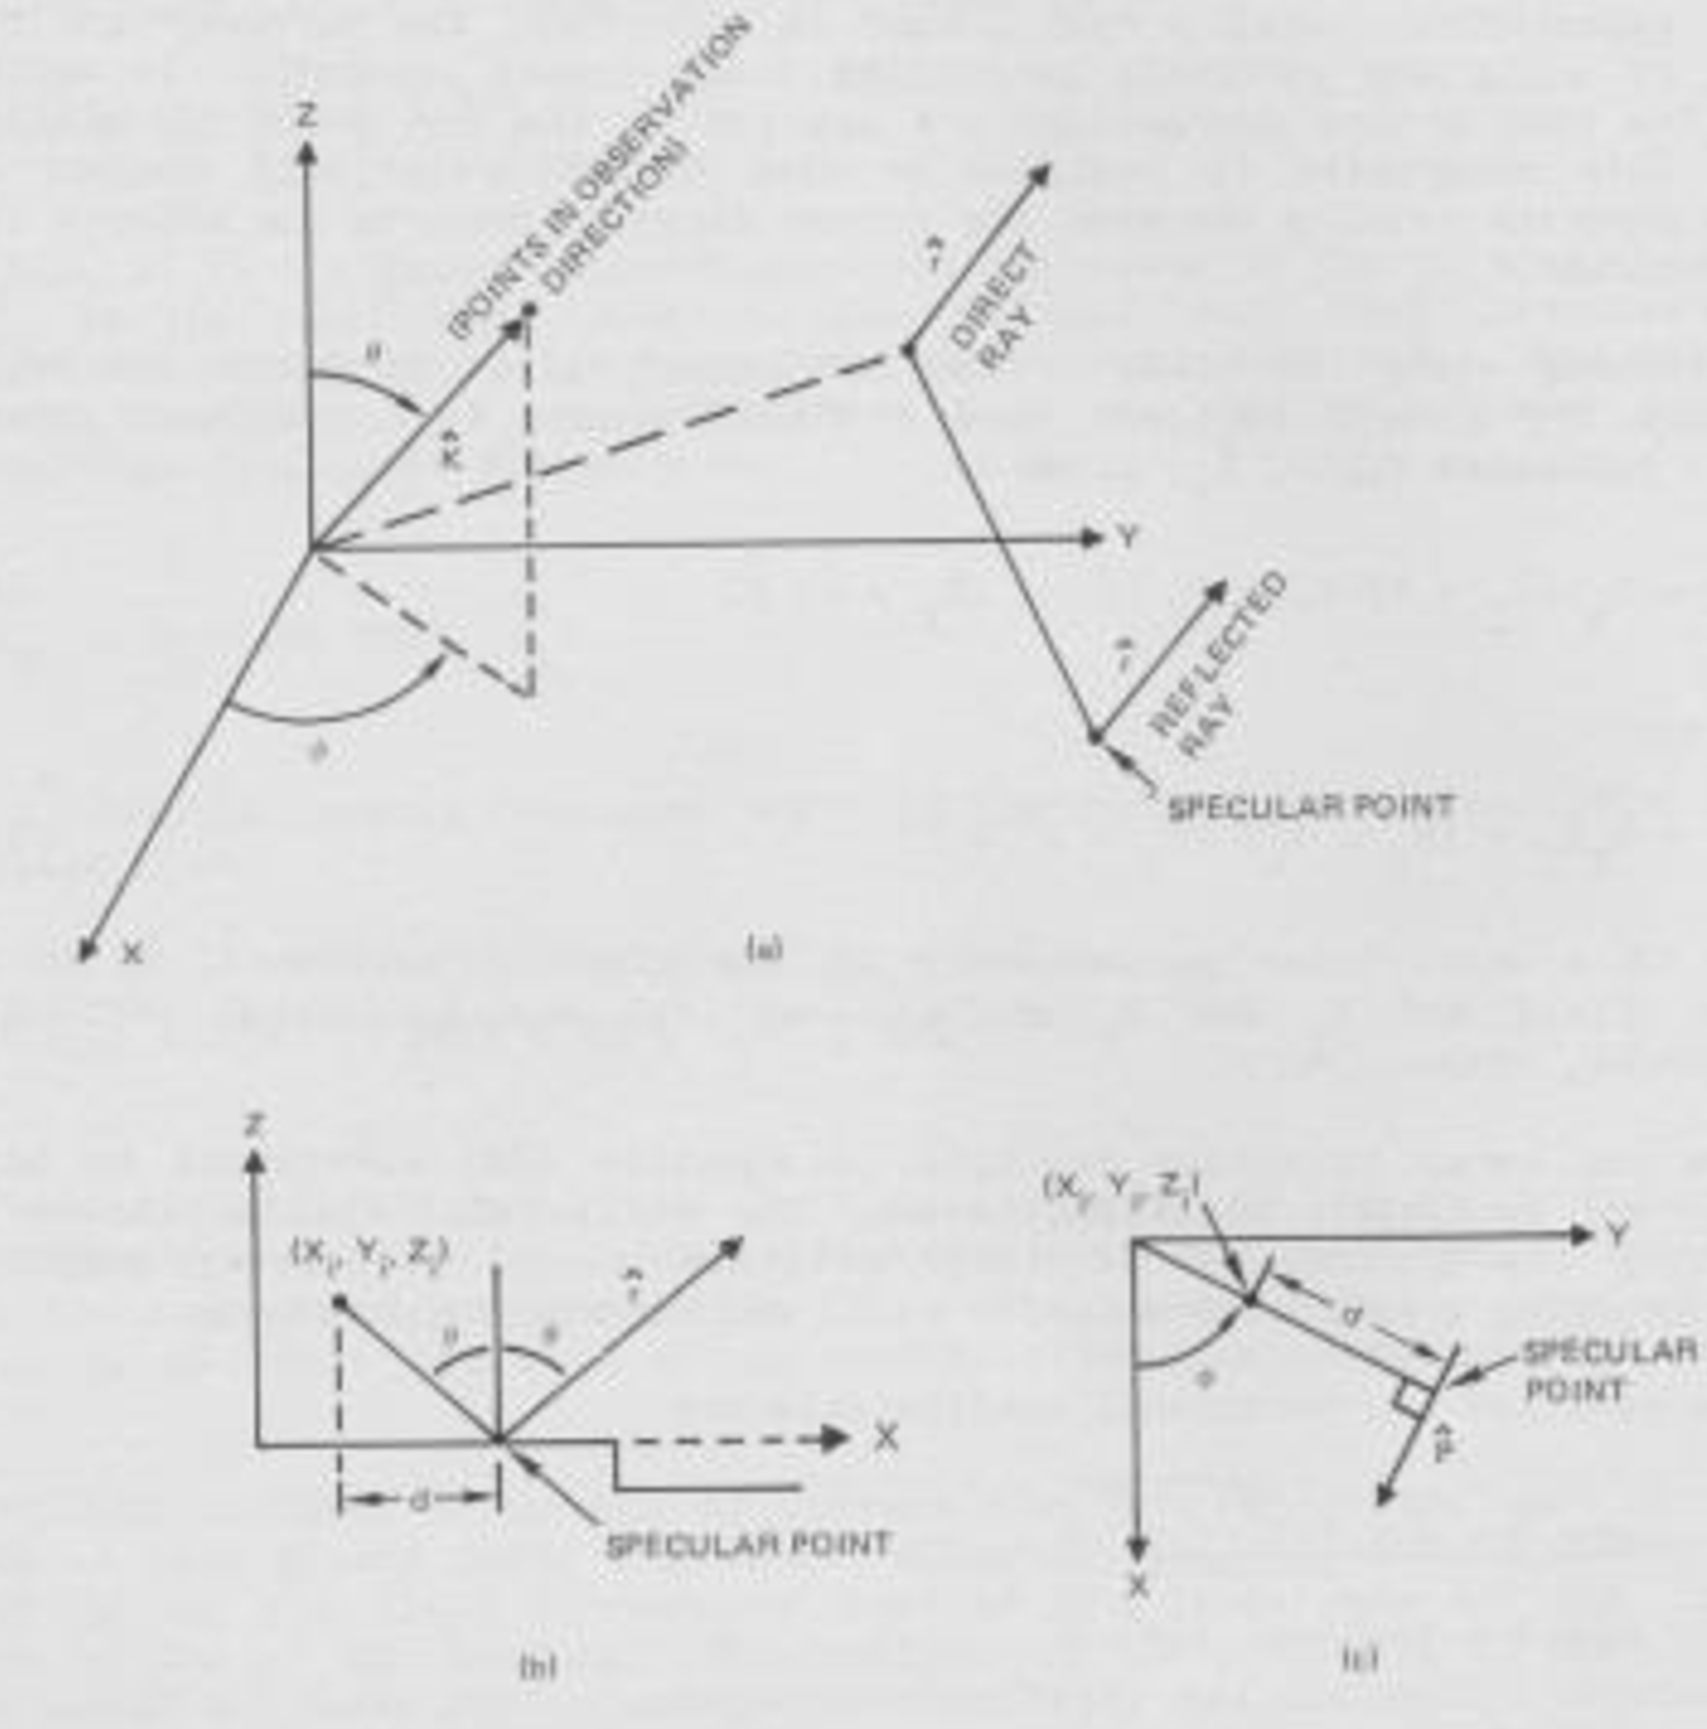
\includegraphics{fig5.eps}}
\caption{Definition of position vectors for Fresnel reflection coefficient}
\label{fig5}
\end{figure}

To obtain the far fields, the integral in equation~\eqref{eq40} implies
the summation over all the current pulses. For the direct field, the
currents and vectors pointing to the current pulse centers are
calculated and stored in arrays by MININEC during the matrix solution
process. The incident field on the ground surface is also computed from
a summation over the currents, but this requires the coordinates of the
specular point (the bounce point). For the geometry illustrated in
Figure~\ref{fig5}, the specular point is given by

\begin{equation}
\bounce{r} = \sqrt{\bounce{x}^2 + \bounce{y}^2}
\label{eq51}
\end{equation}

\begin{equation}
\bounce{x} = x_i + d\cos\phi
\label{eq52}
\end{equation}

\begin{equation}
\bounce{y} = y_i + d\sin\phi
\label{eq53}
\end{equation}

\begin{equation}
d = Z_i \tan\theta
\label{eq54}
\end{equation}

The value of $\bounce{x}$ or $\bounce{r}$ is used
appropriately for the case of linear or circular zone boundaries to
determine in which media the bounce occurs. The height of the ground at
this point is used to locate the image of the source.

The ground surface impedance in any zone is given by

\begin{equation}
Z_g = \frac{1}{\sqrt{\frac{\varepsilon}{\varepsilon_0}
                    - j\frac{\sigma}{\omega\varepsilon_0}}}
\label{eq55}
\end{equation}

The surface impedance, when a ground screen is present and the specular
point lies on the ground screen, is given by Wait
\cite{r14}, (also see \cite{r4}). The impedance of
the ground screen by itself is

\[
Z_{gs} (\bounce{r}) = j\sqrt{\varepsilon_0\mu_0}\,
\frac{\omega\bounce{r}}{N} \ln \frac{\bounce{r}}{NC_0}
\]

\noindent
where $N$ is the number of wires in the ground screen and $C_0$ is the
radius of each wire. The effective ground impedance is formed by
computing the parallel impedance of the ground without the ground screen
and the impedance of the ground screen without the ground, or

\begin{equation}
Z = \frac{Z_g Z_{gs}}{Z_g + Z_{gs}}
\label{eq56}
\end{equation}

\noindent (where $Z=Z_g$ if no ground screen is present).

The total field at a point $(\theta,\phi,r)$ is the vector sum of the
direct and reflected fields as described. When the range $r$
is set to zero or the power gain option is selected, the
$e^{-jkr} / r$ term is set to unity. The total resulting field is used
in equation~\eqref{eq43} to calculate the power gain.

\section{Validation and Modeling Guidance}
\label{sec-validation}
The solution to an antenna problem generated by a method of moments
computer program is, at best, an approximation. How close the solution
is to reality depends in part on (1) the numerical methods employed in
the code (and how well these methods are implemented), (2) the inherent
accuracy (i.e., the number of significant digits) of the computer, (3)
how well the antenna being modeled conforms to the limitations (i.e.,
simplifying assumptions) of the electromagnetics formulation used to
create the computer program, and (4) the user's experience. Nonetheless,
highly acurate answers can be obtained by careful modeling of the
antenna configuration, taking into account the inherent limitations of
the computer program.

\begin{sidewaysfigure}[htb]
\centerline{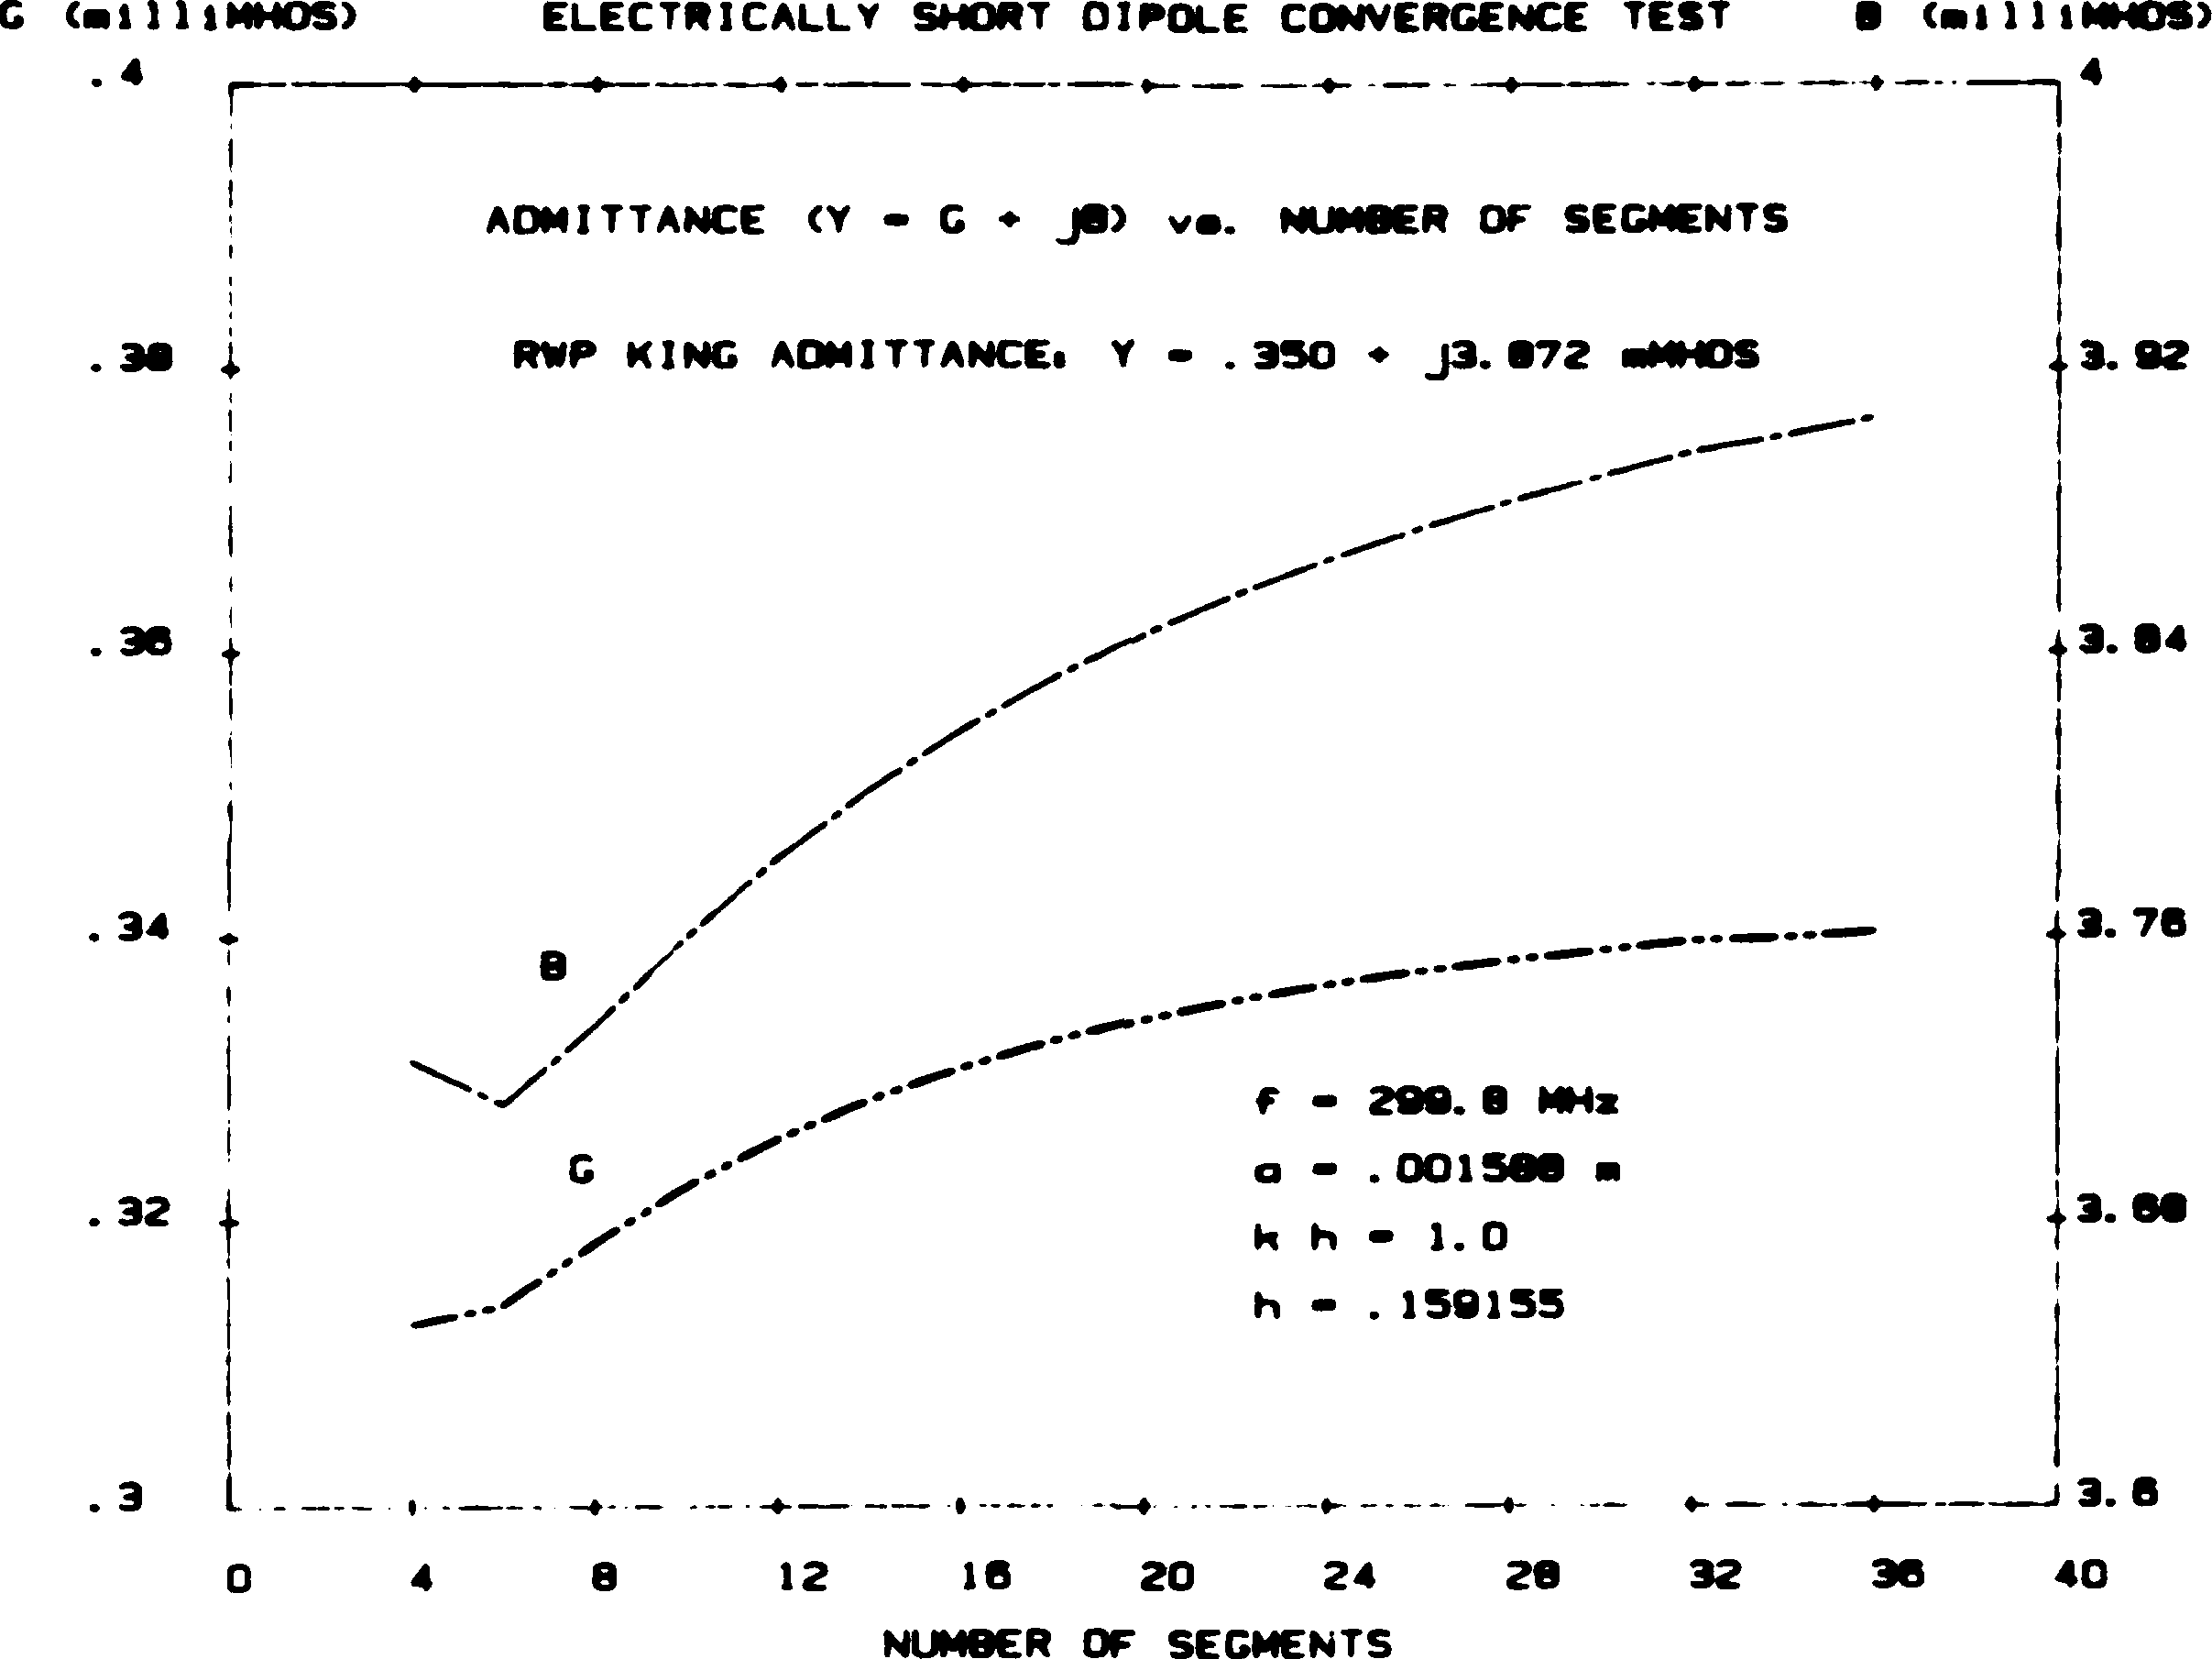
\includegraphics{fig6.eps}}
\caption{Convergence test for an electrically short dipole when
admittance is given (Part a)}
\label{fig6}
\end{sidewaysfigure}

\begin{sidewaysfigure}[htb]
\centerline{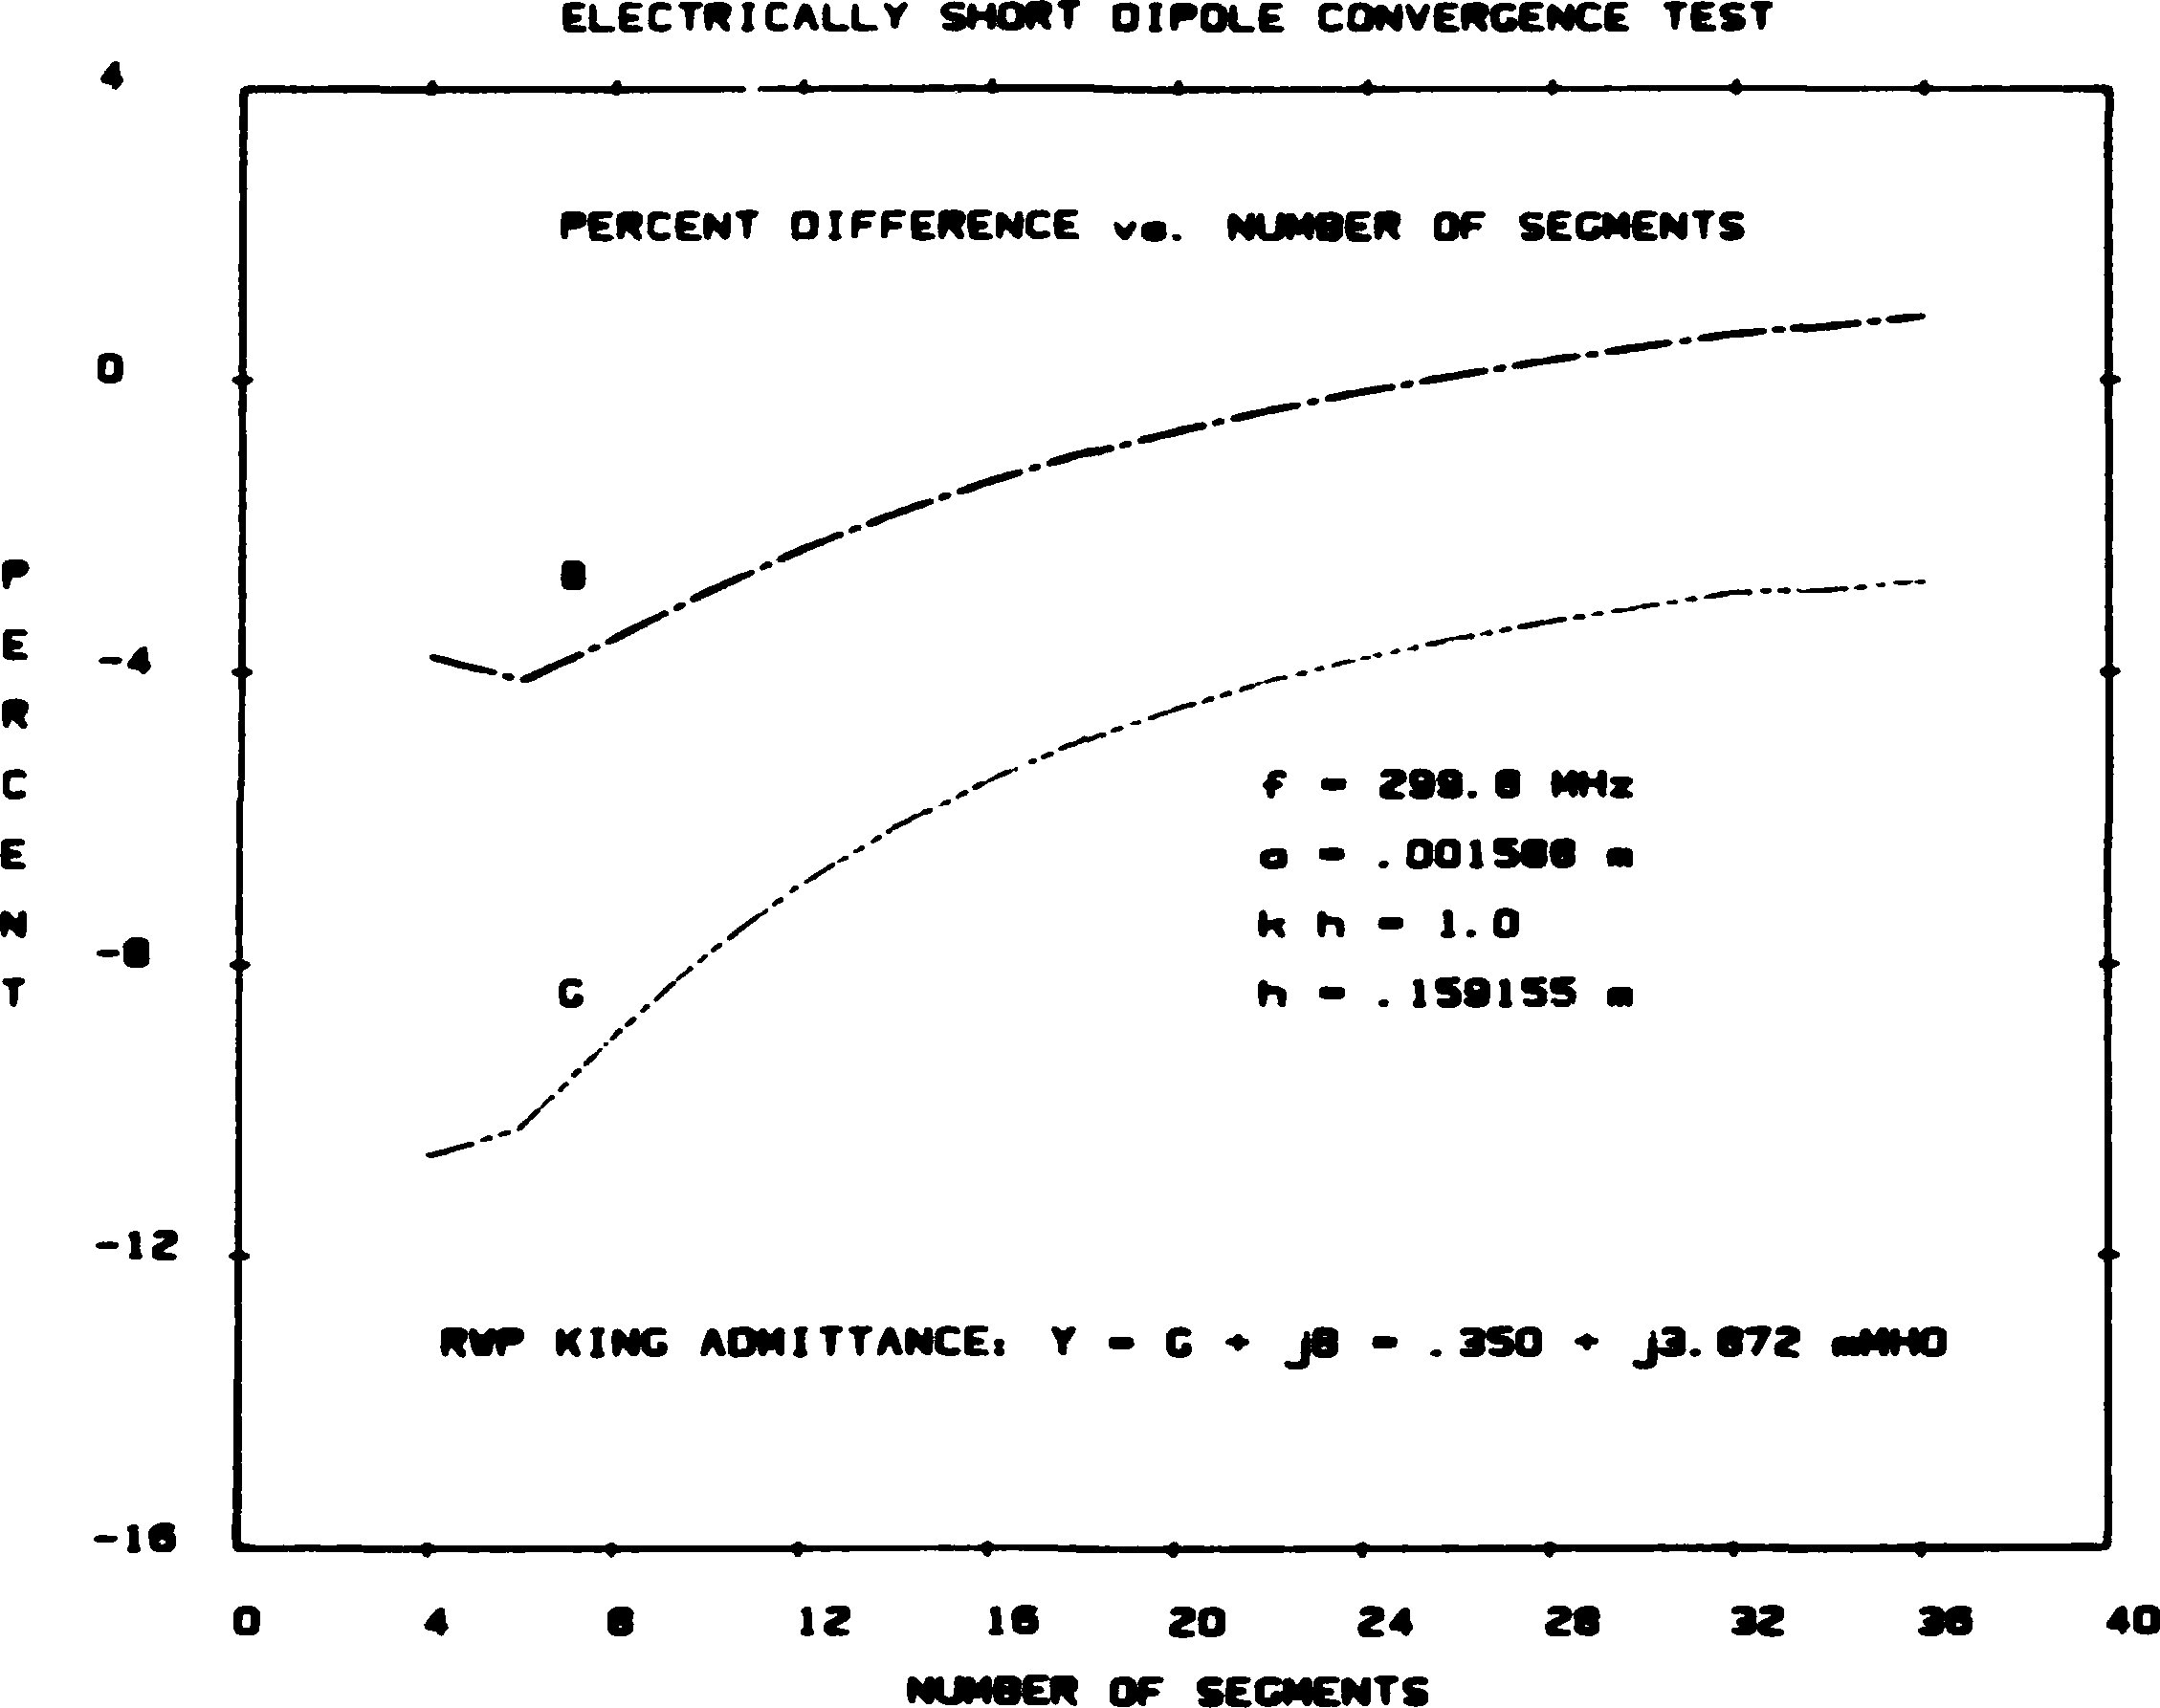
\includegraphics{fig7.eps}}
\caption{Convergence test for an electrically short dipole showing the
percent difference in admittance between MININEC and R. W. P. King
\cite{r8}, \cite{r9} (Part b)}
\label{fig7}
\end{sidewaysfigure}

\begin{sidewaysfigure}[htb]
\centerline{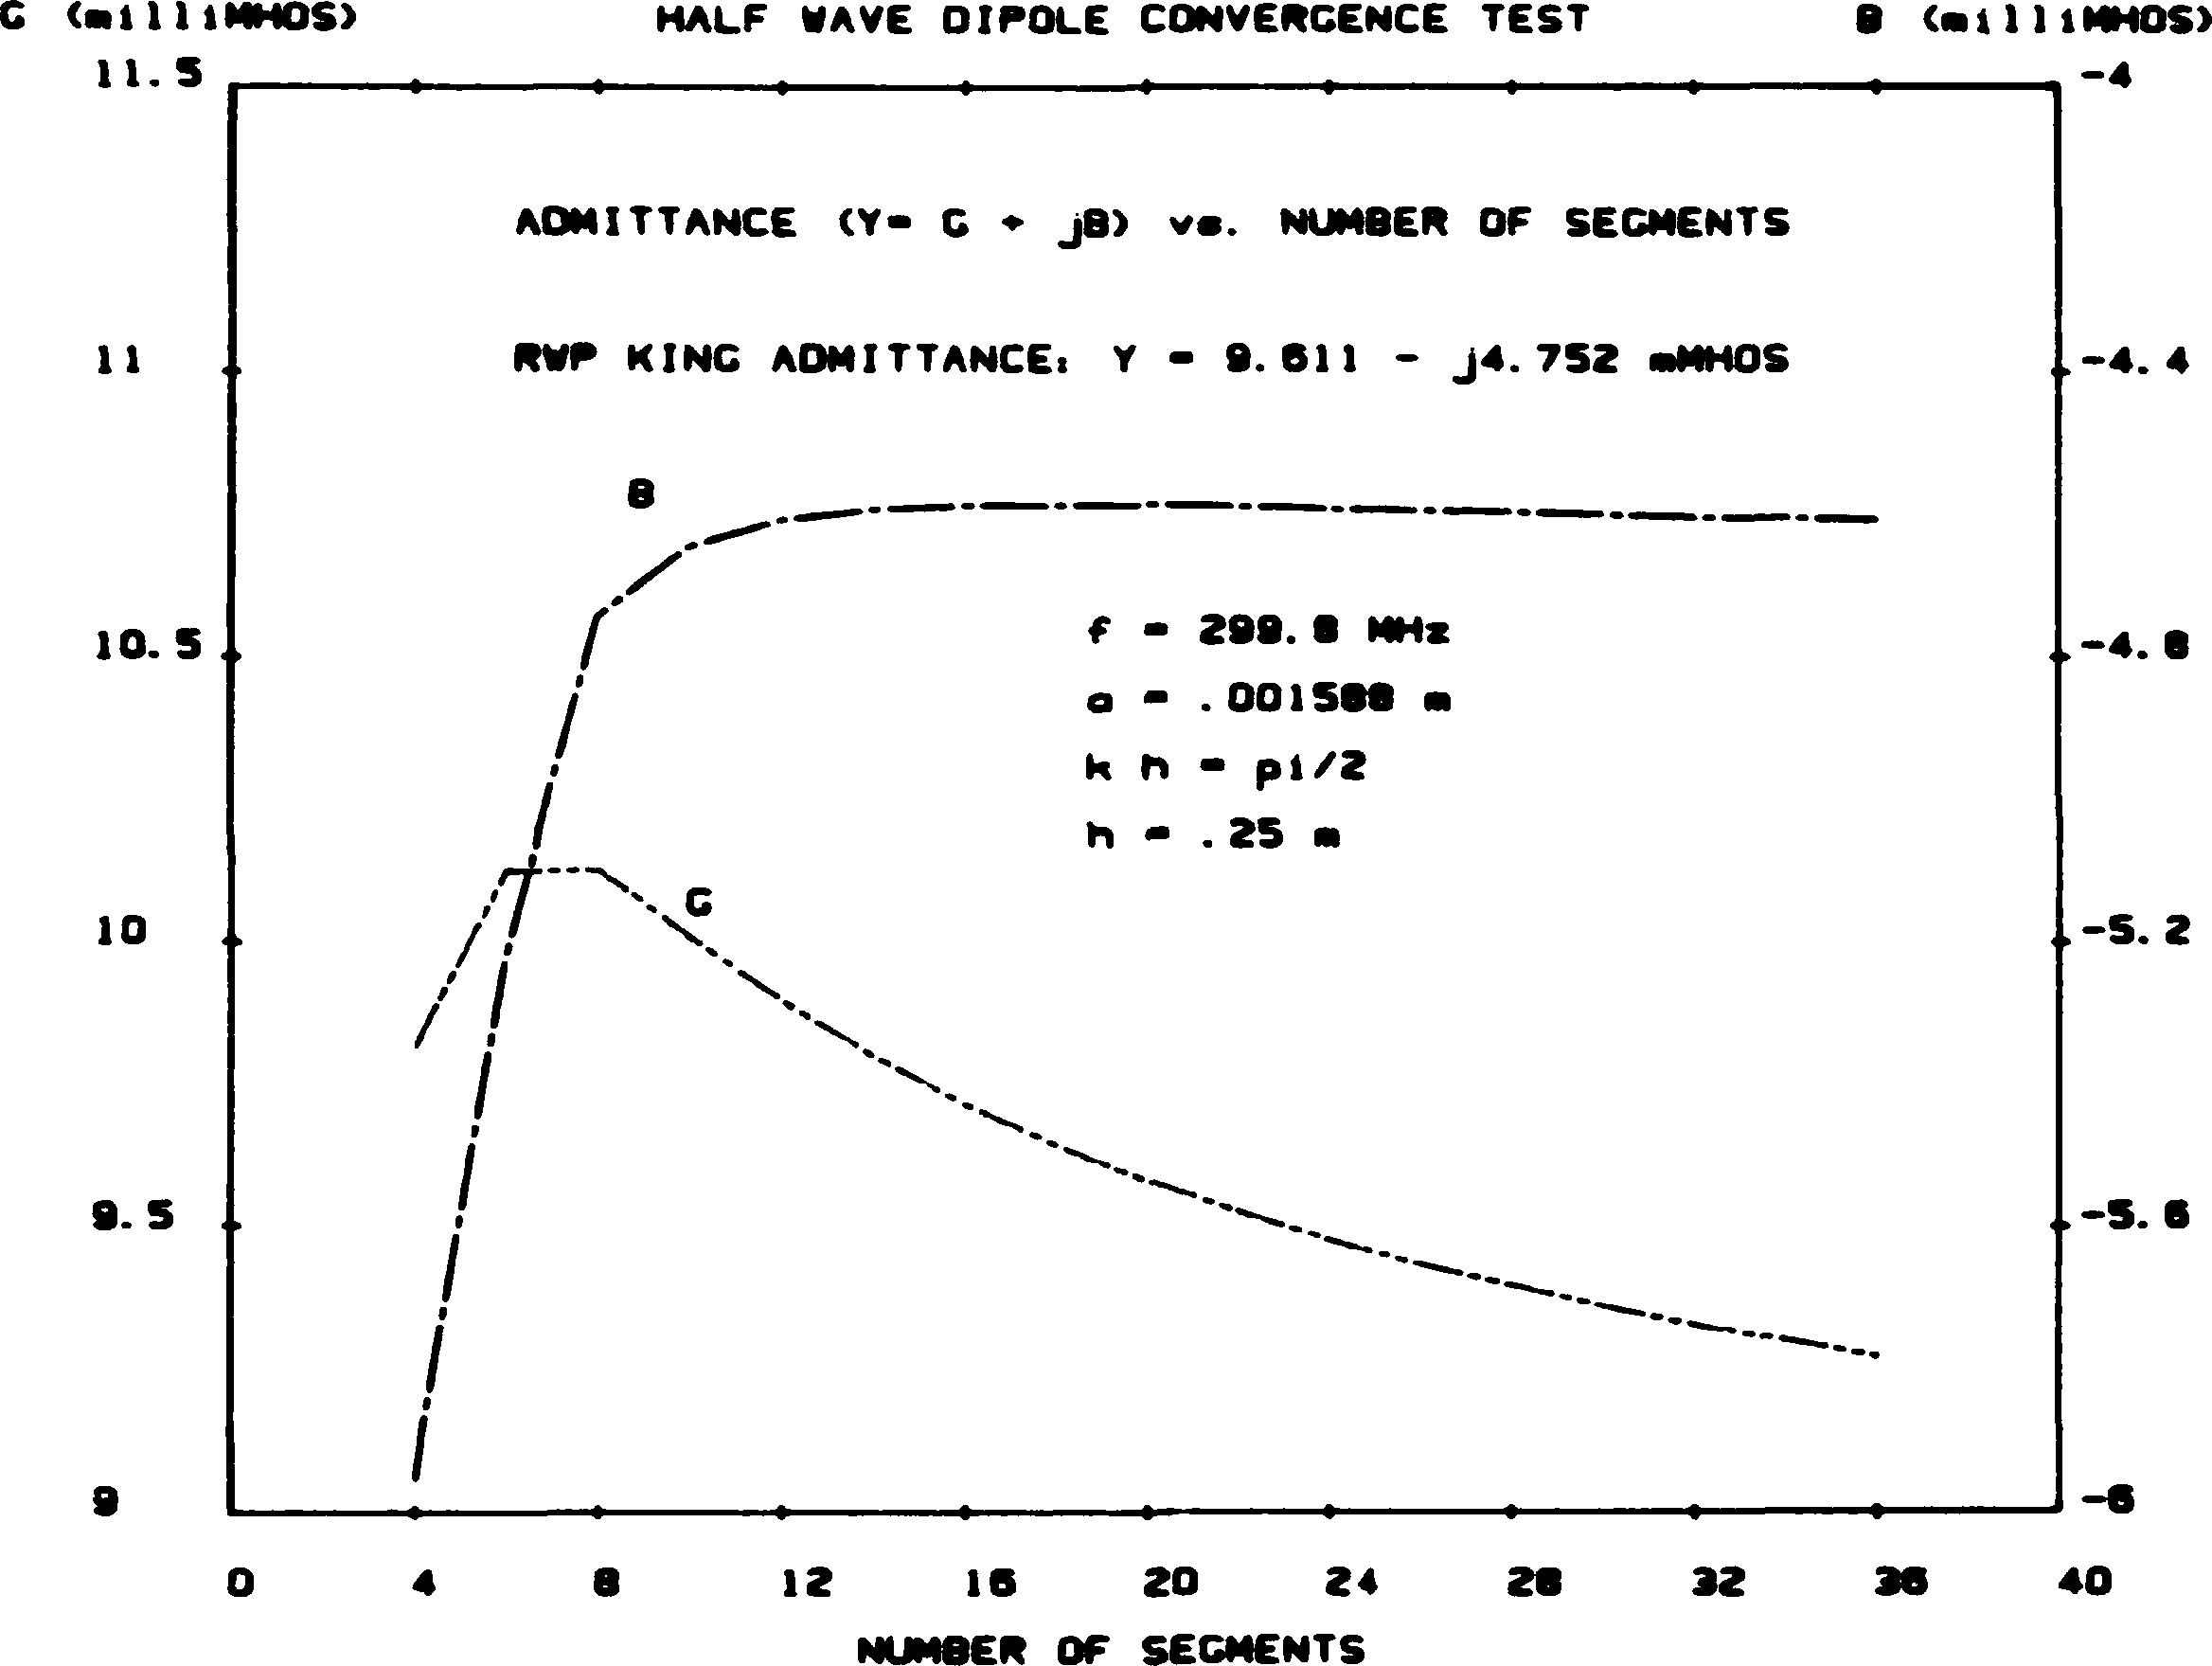
\includegraphics{fig8.eps}}
\caption{Convergence test for a half wave dipole when admittance is
given (Part a)}
\label{fig8}
\end{sidewaysfigure}

\begin{sidewaysfigure}[htb]
\centerline{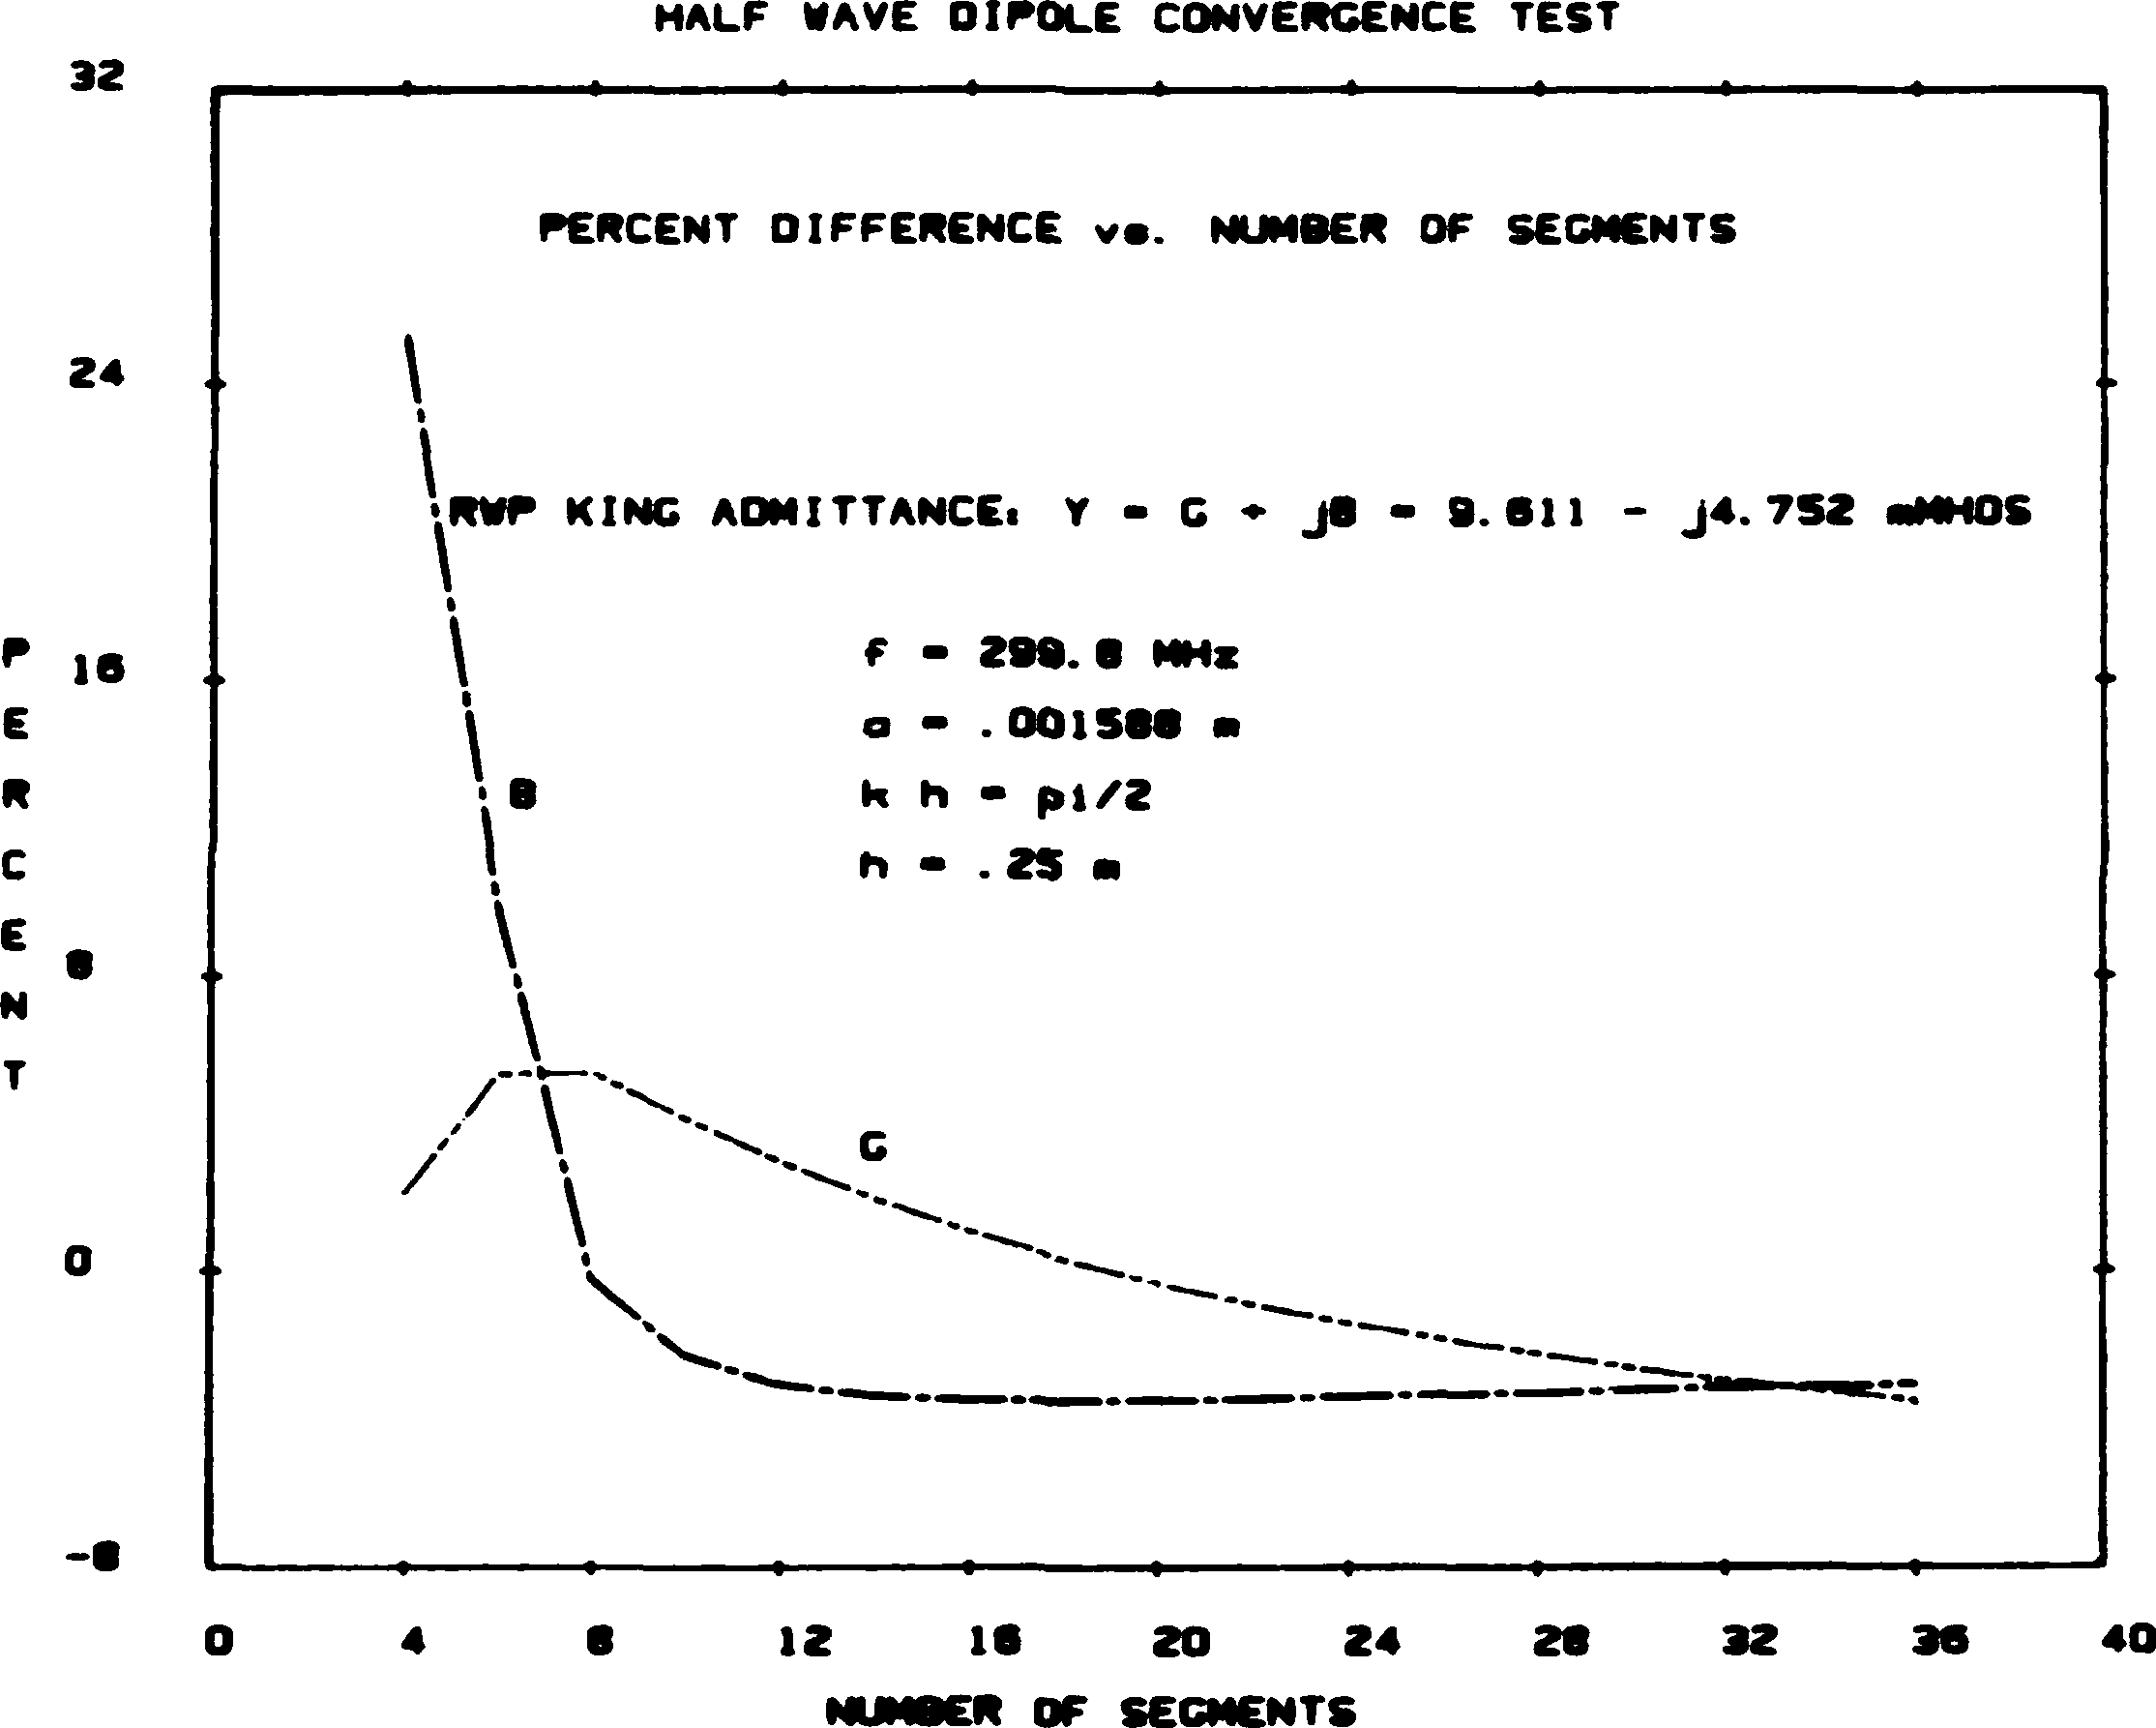
\includegraphics{fig9.eps}}
\caption{Convergence test for a half wave dipole showing the percent
difference in admittance between MININEC and R. W. P. King
\cite{r8}, \cite{r9} (Part b)}
\label{fig9}
\end{sidewaysfigure}

\begin{sidewaysfigure}[htb]
\centerline{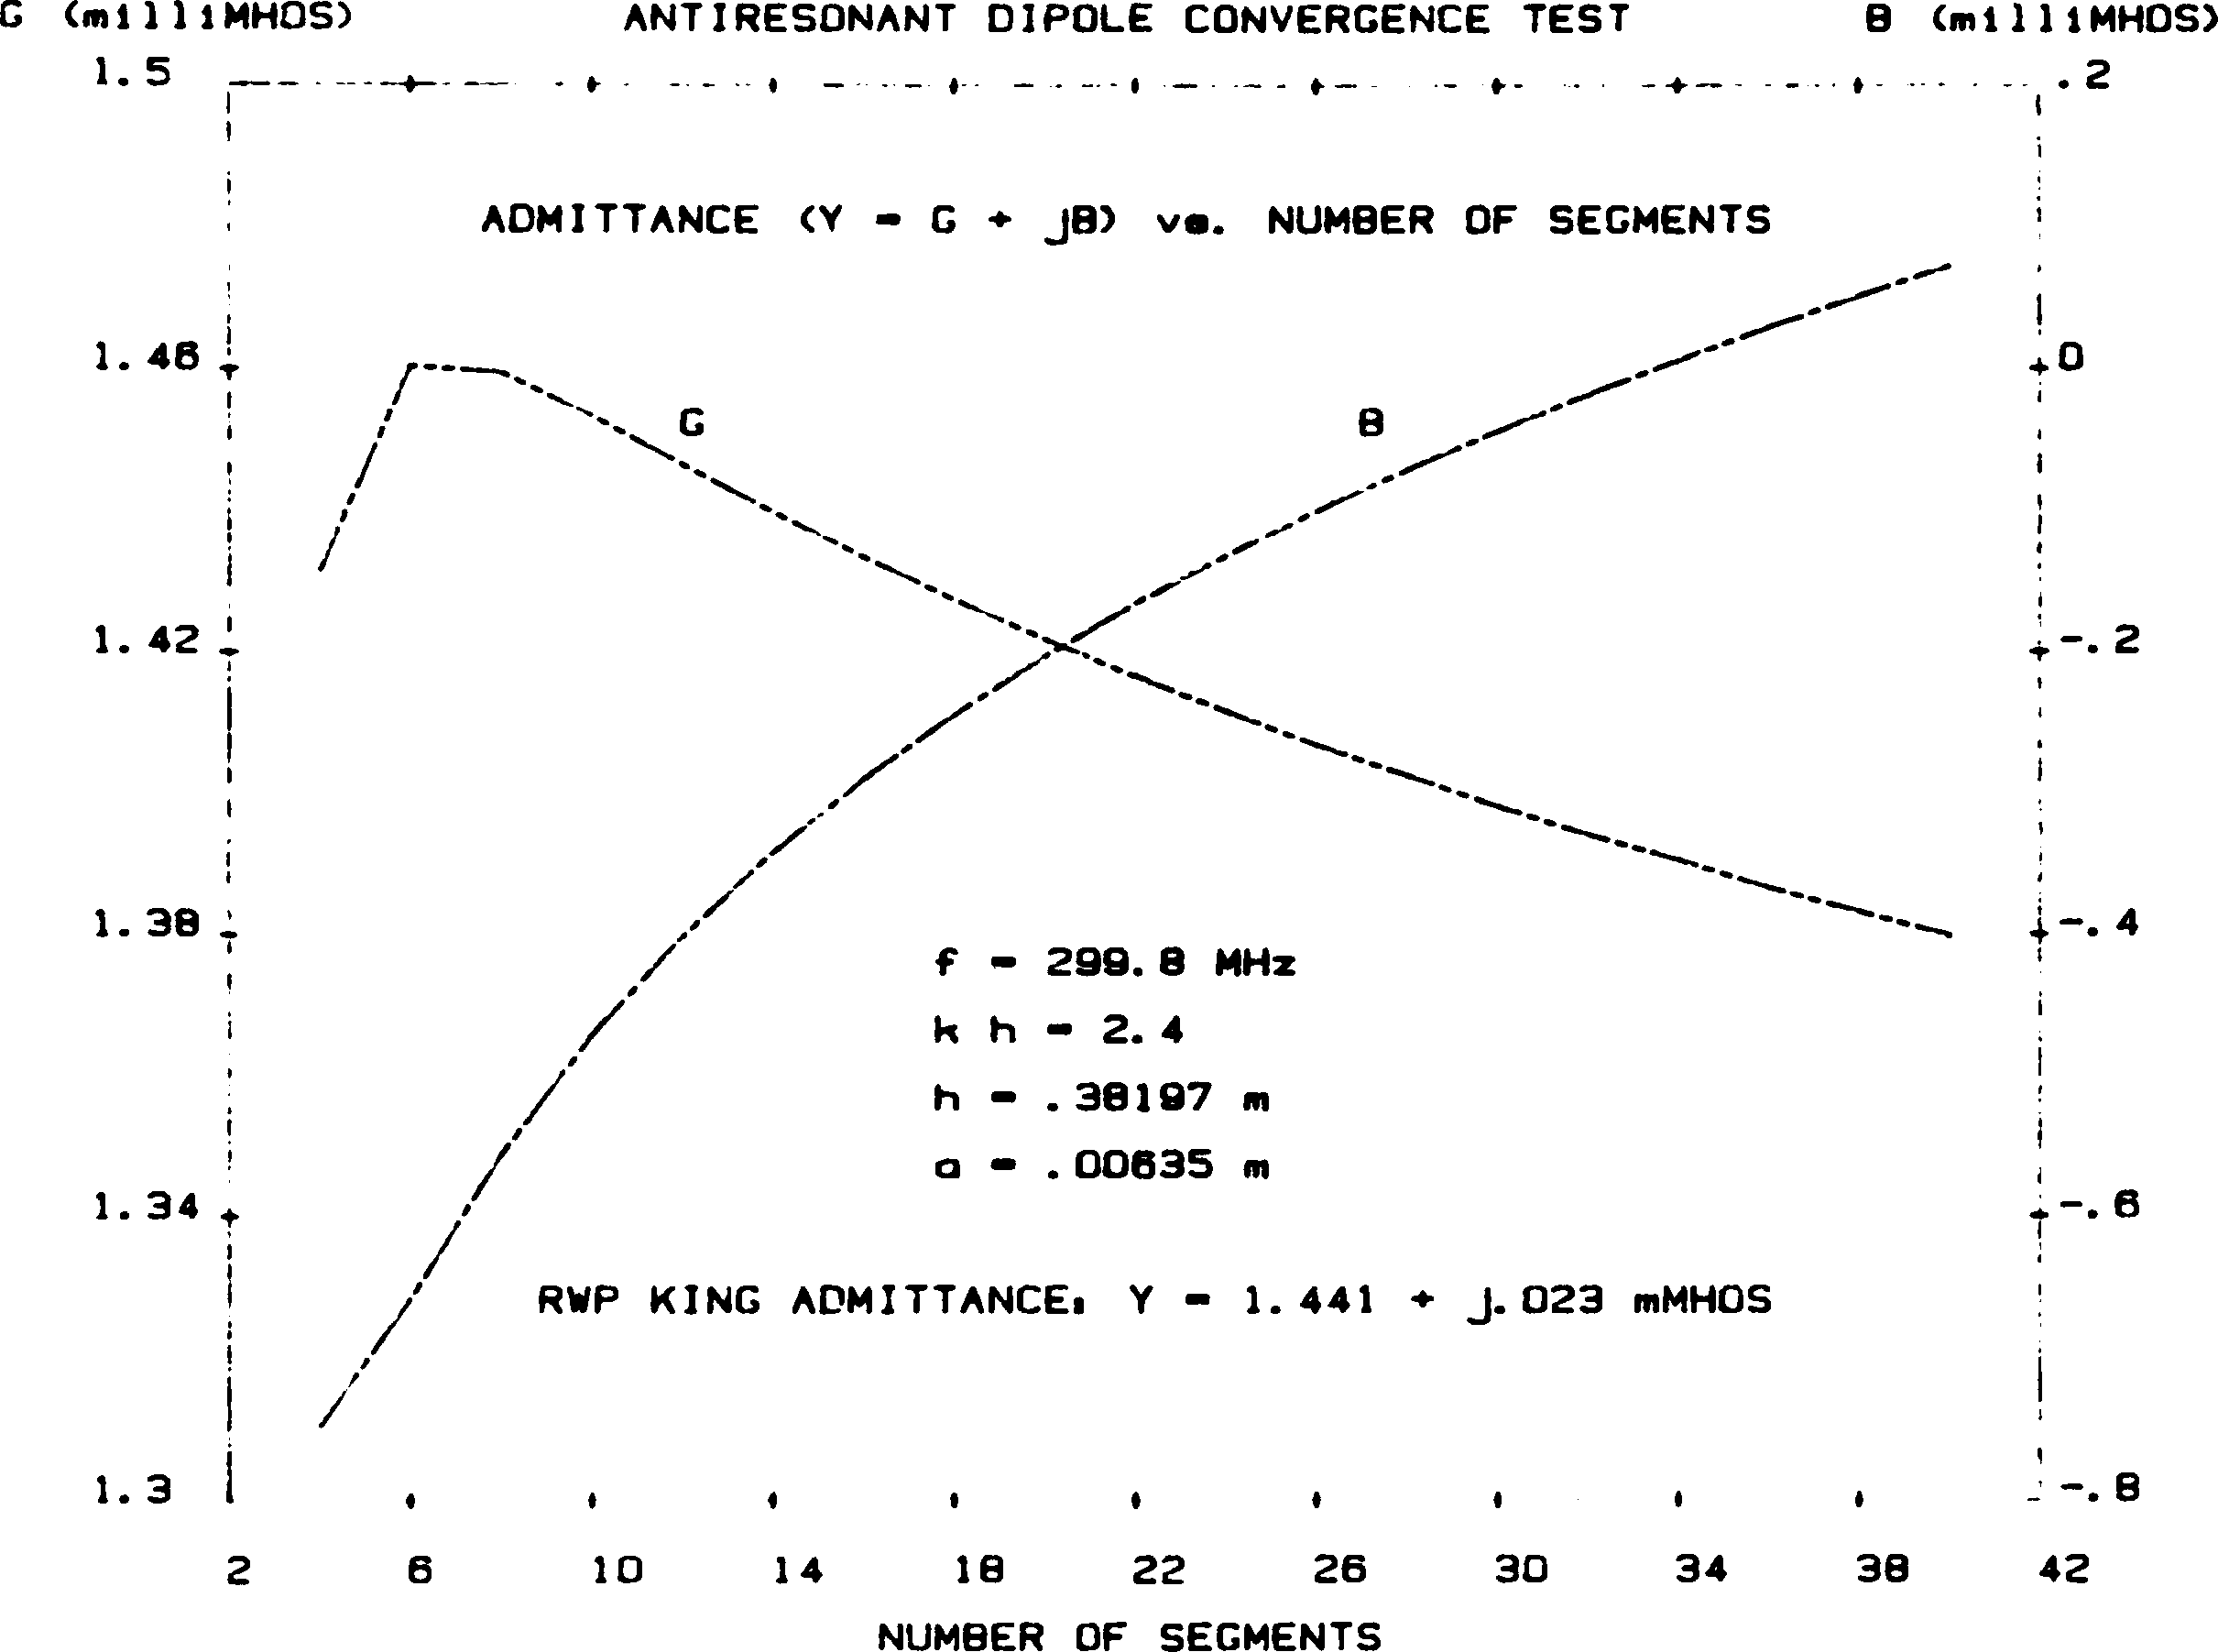
\includegraphics{fig10.eps}}
\caption{Convergence test for an antiresonant dipole when admittance is
given (Part a)}
\label{fig10}
\end{sidewaysfigure}

\begin{sidewaysfigure}[htb]
\centerline{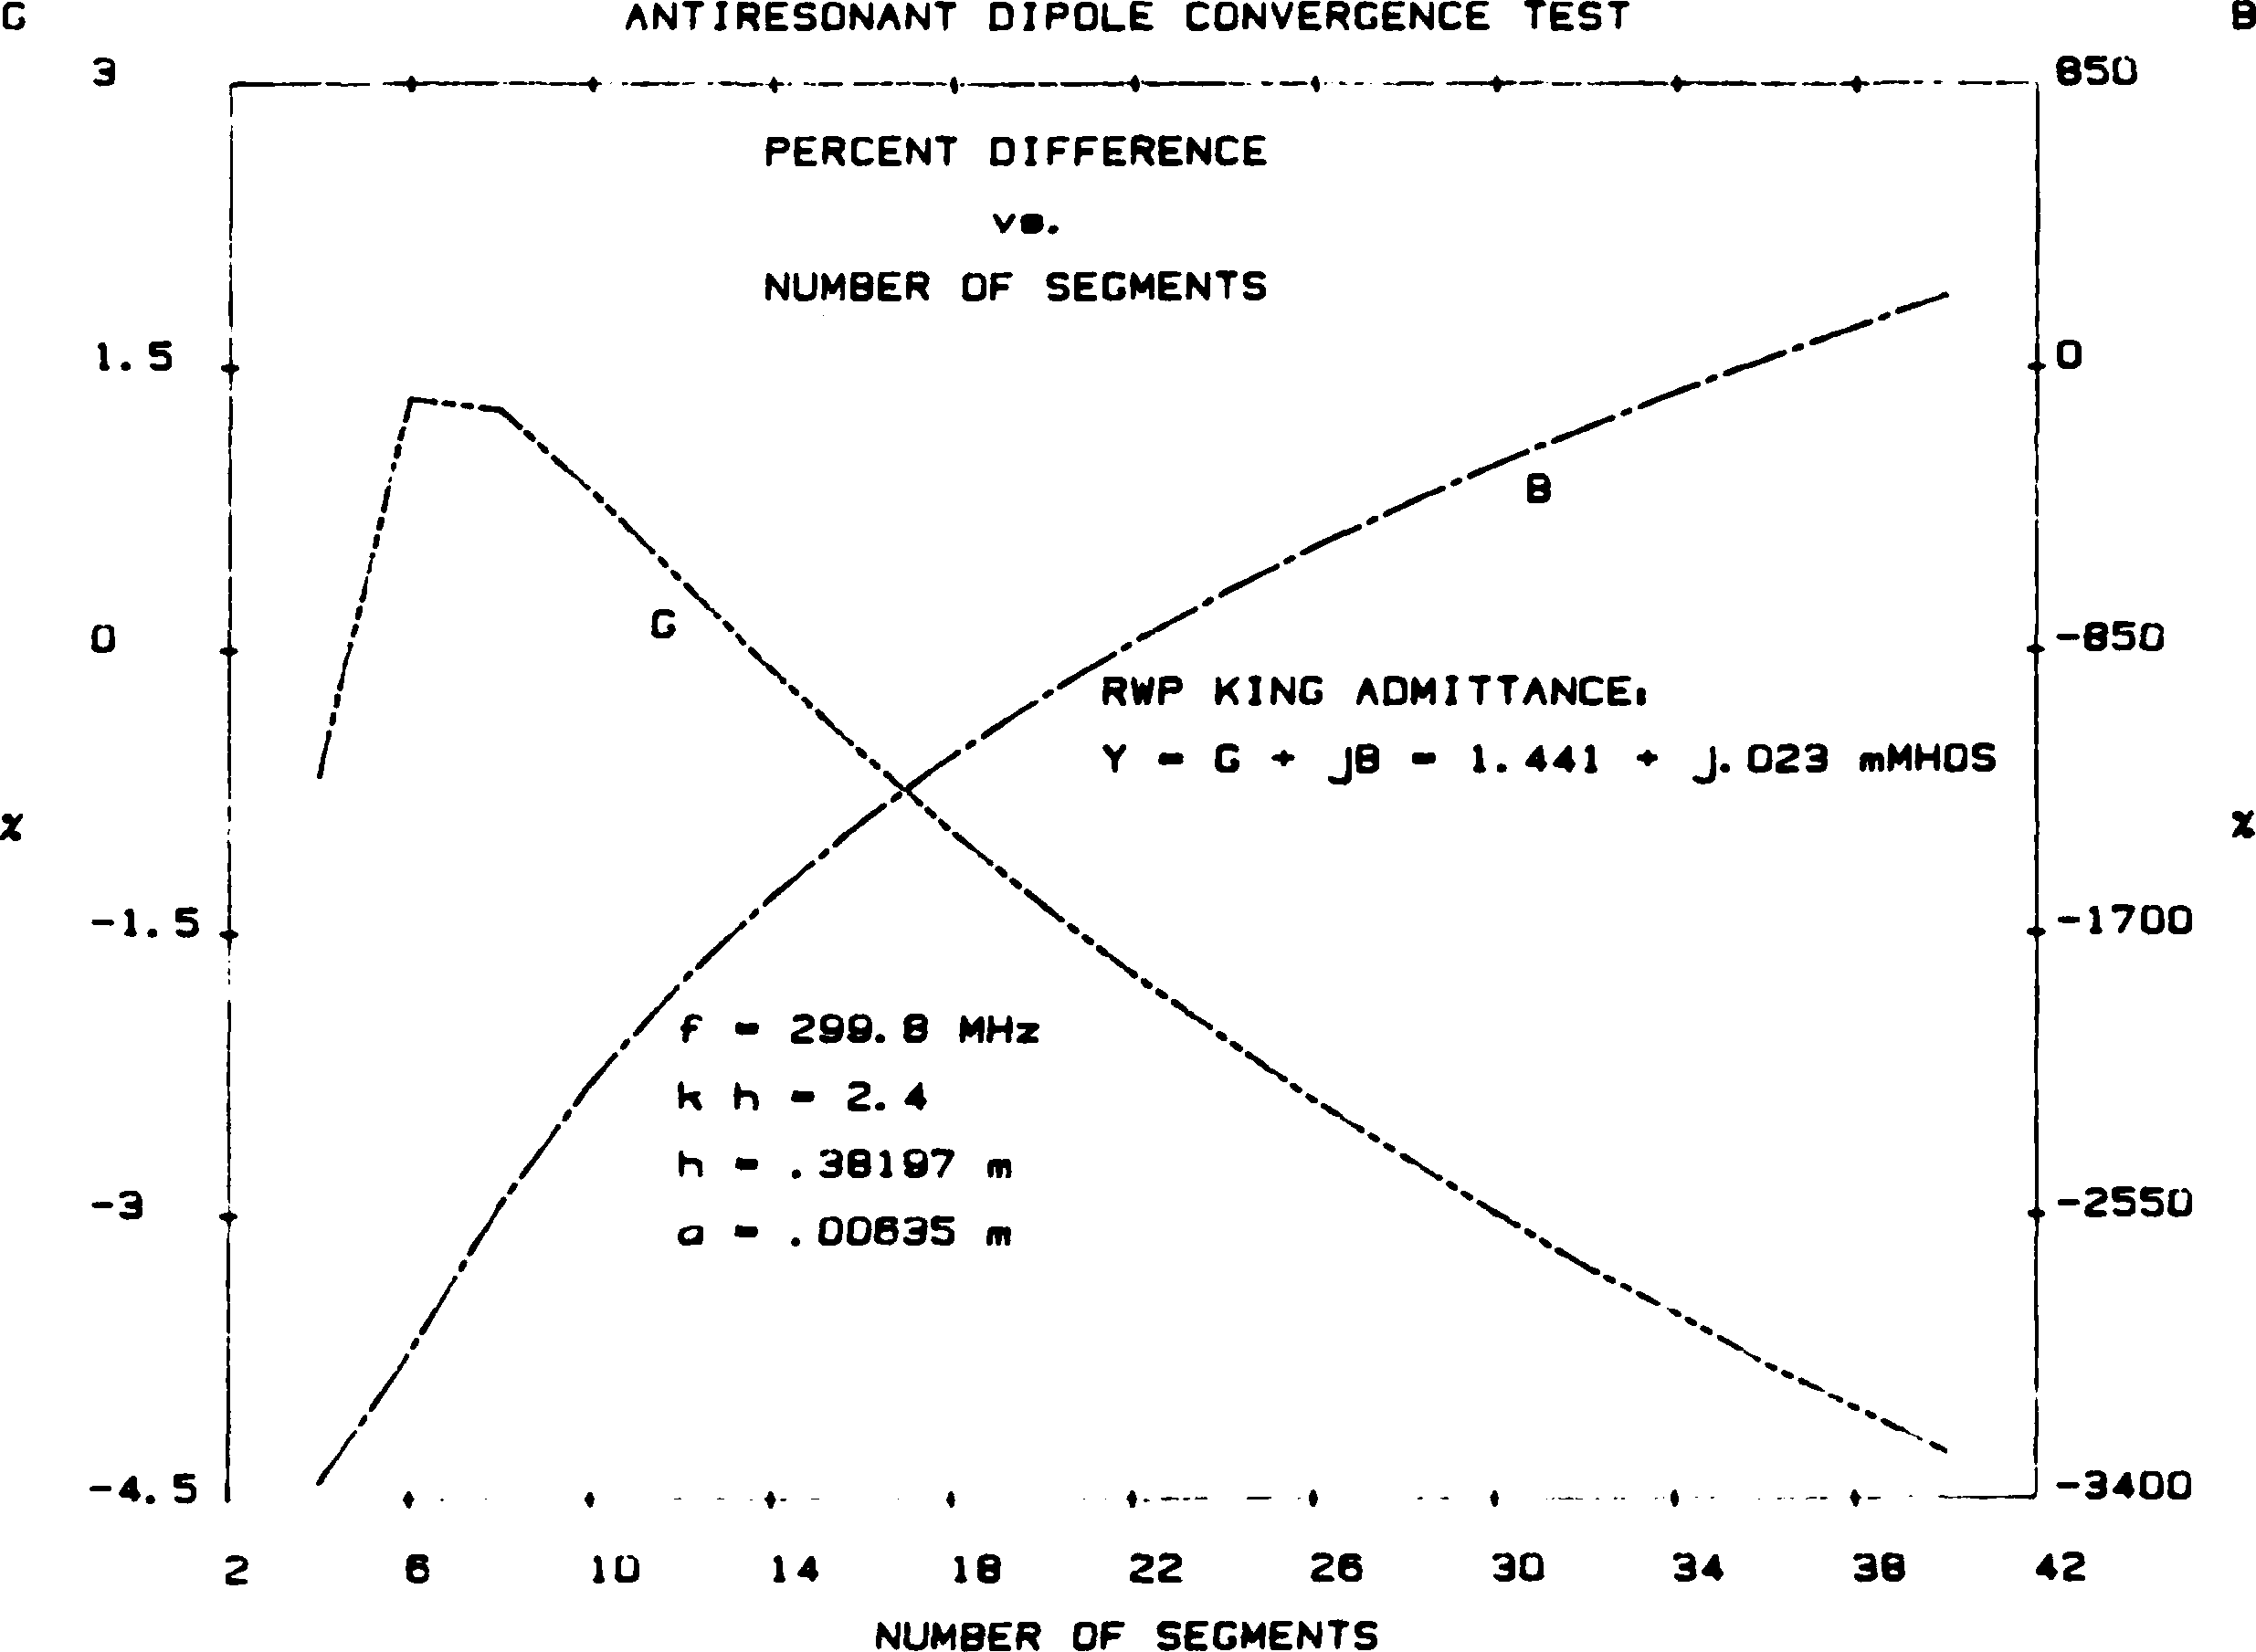
\includegraphics{fig11.eps}}
\caption{Convergence test for an antiresonant dipole showing the percent
difference in admittance between MININEC and R. W. P. King
\cite{r8}, \cite{r9} (Part b)}
\label{fig11}
\end{sidewaysfigure}
\afterpage\clearpage

\begin{sidewaysfigure}[htb]
\centerline{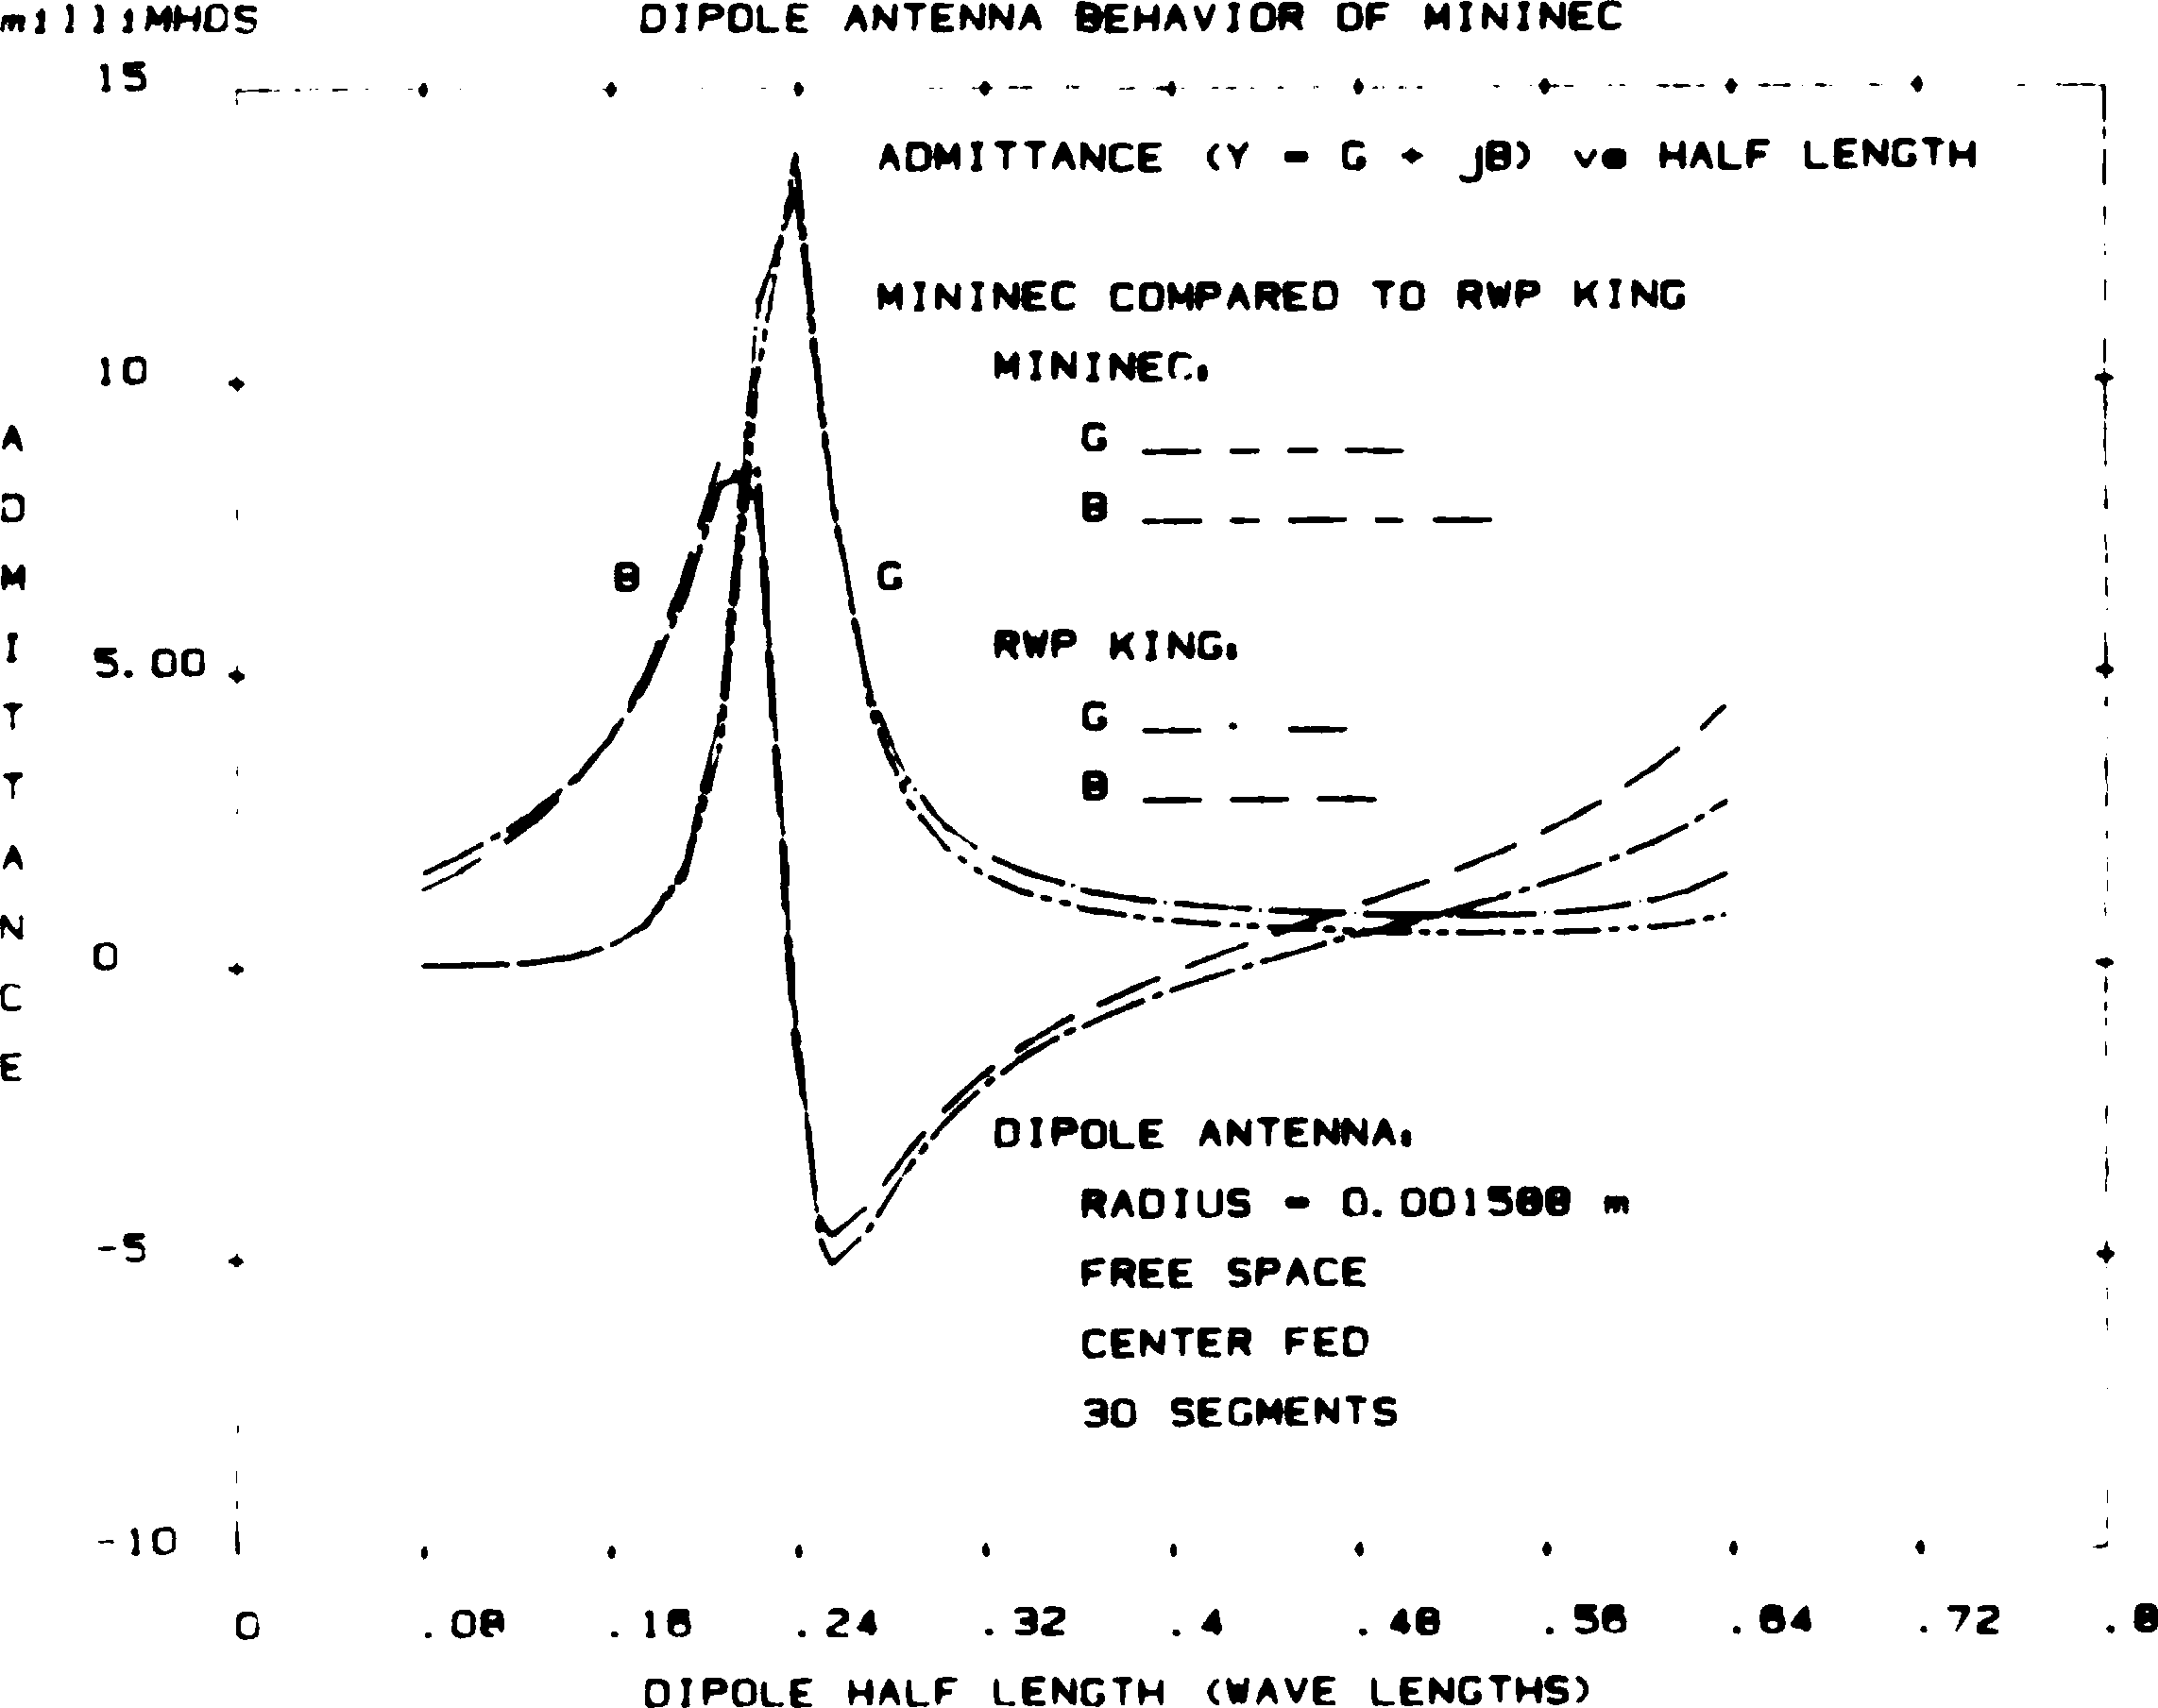
\includegraphics{fig12.eps}}
\caption{Dipole admittance predicted by MININEC (compared to the theory of
R. W. P. King \cite{r8},~\cite{r9})}
\label{fig12}
\end{sidewaysfigure}

\begin{sidewaysfigure}[htb]
\centerline{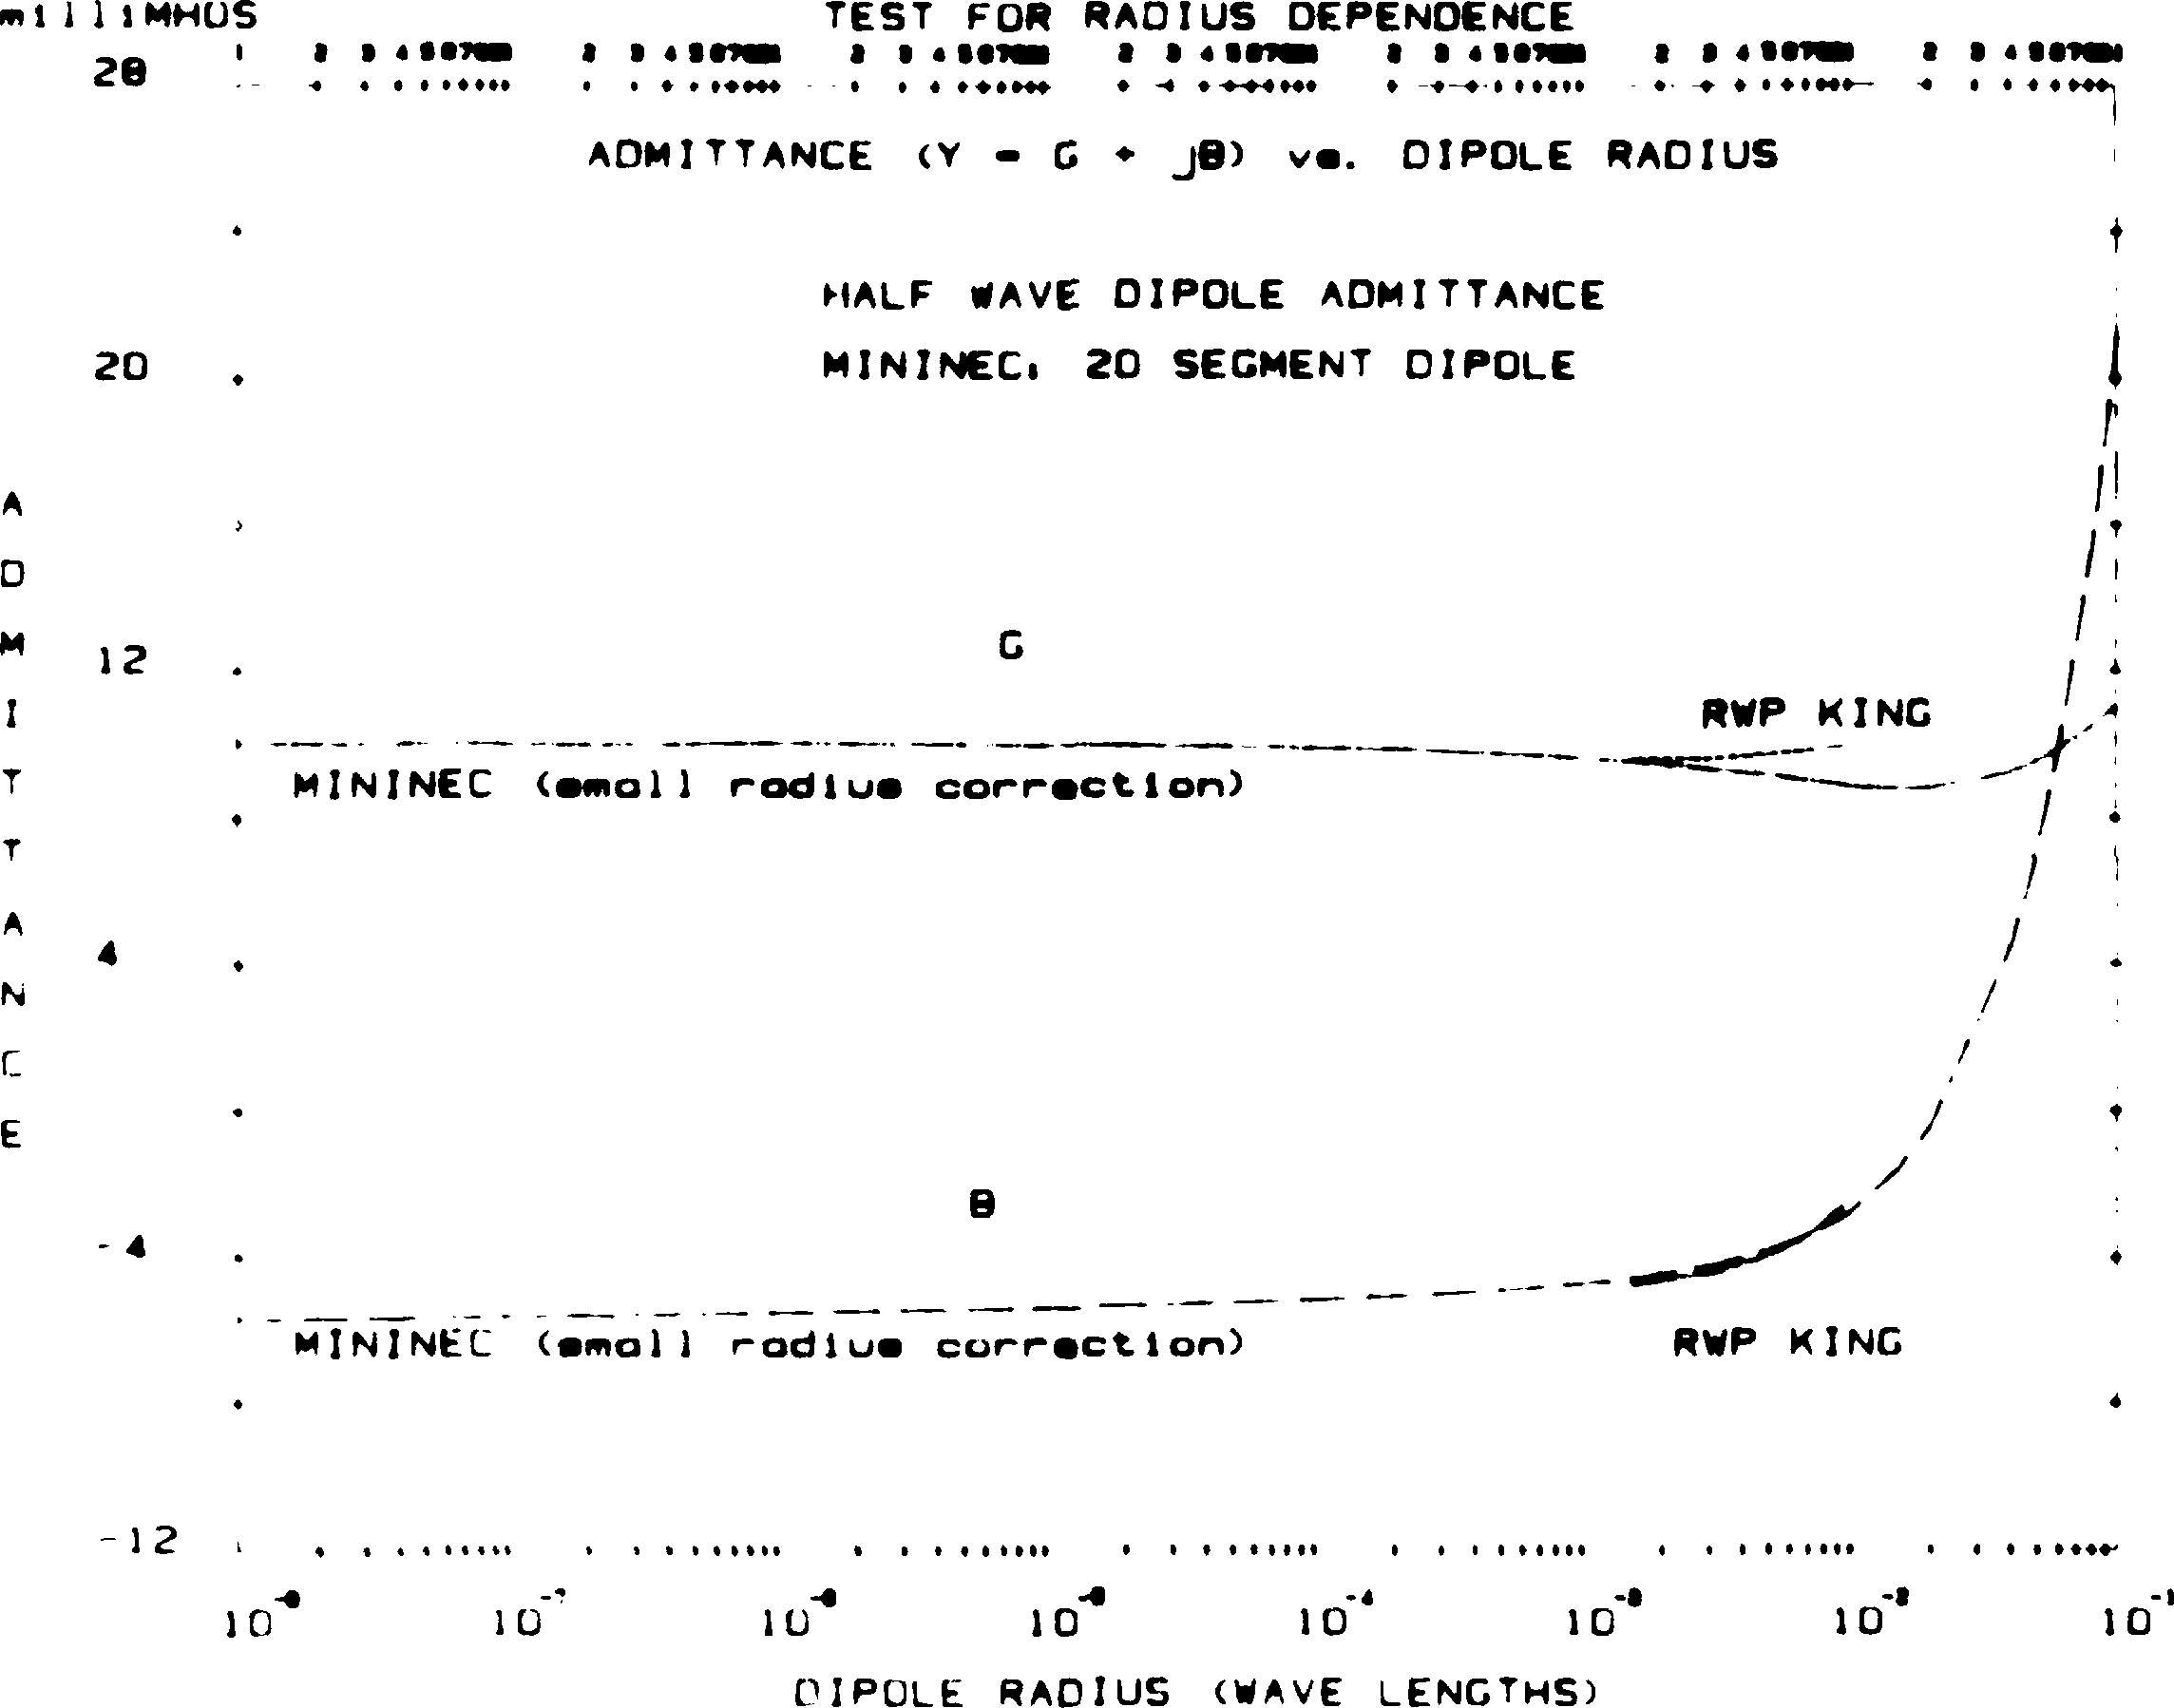
\includegraphics{fig13.eps}}
\caption{[Dipole admittance vs. Wire Radius] (compared to the theory of
R. W. P. King \cite{r8},~\cite{r9})}
\label{fig13}
\end{sidewaysfigure}

\begin{sidewaysfigure}[htb]
\centerline{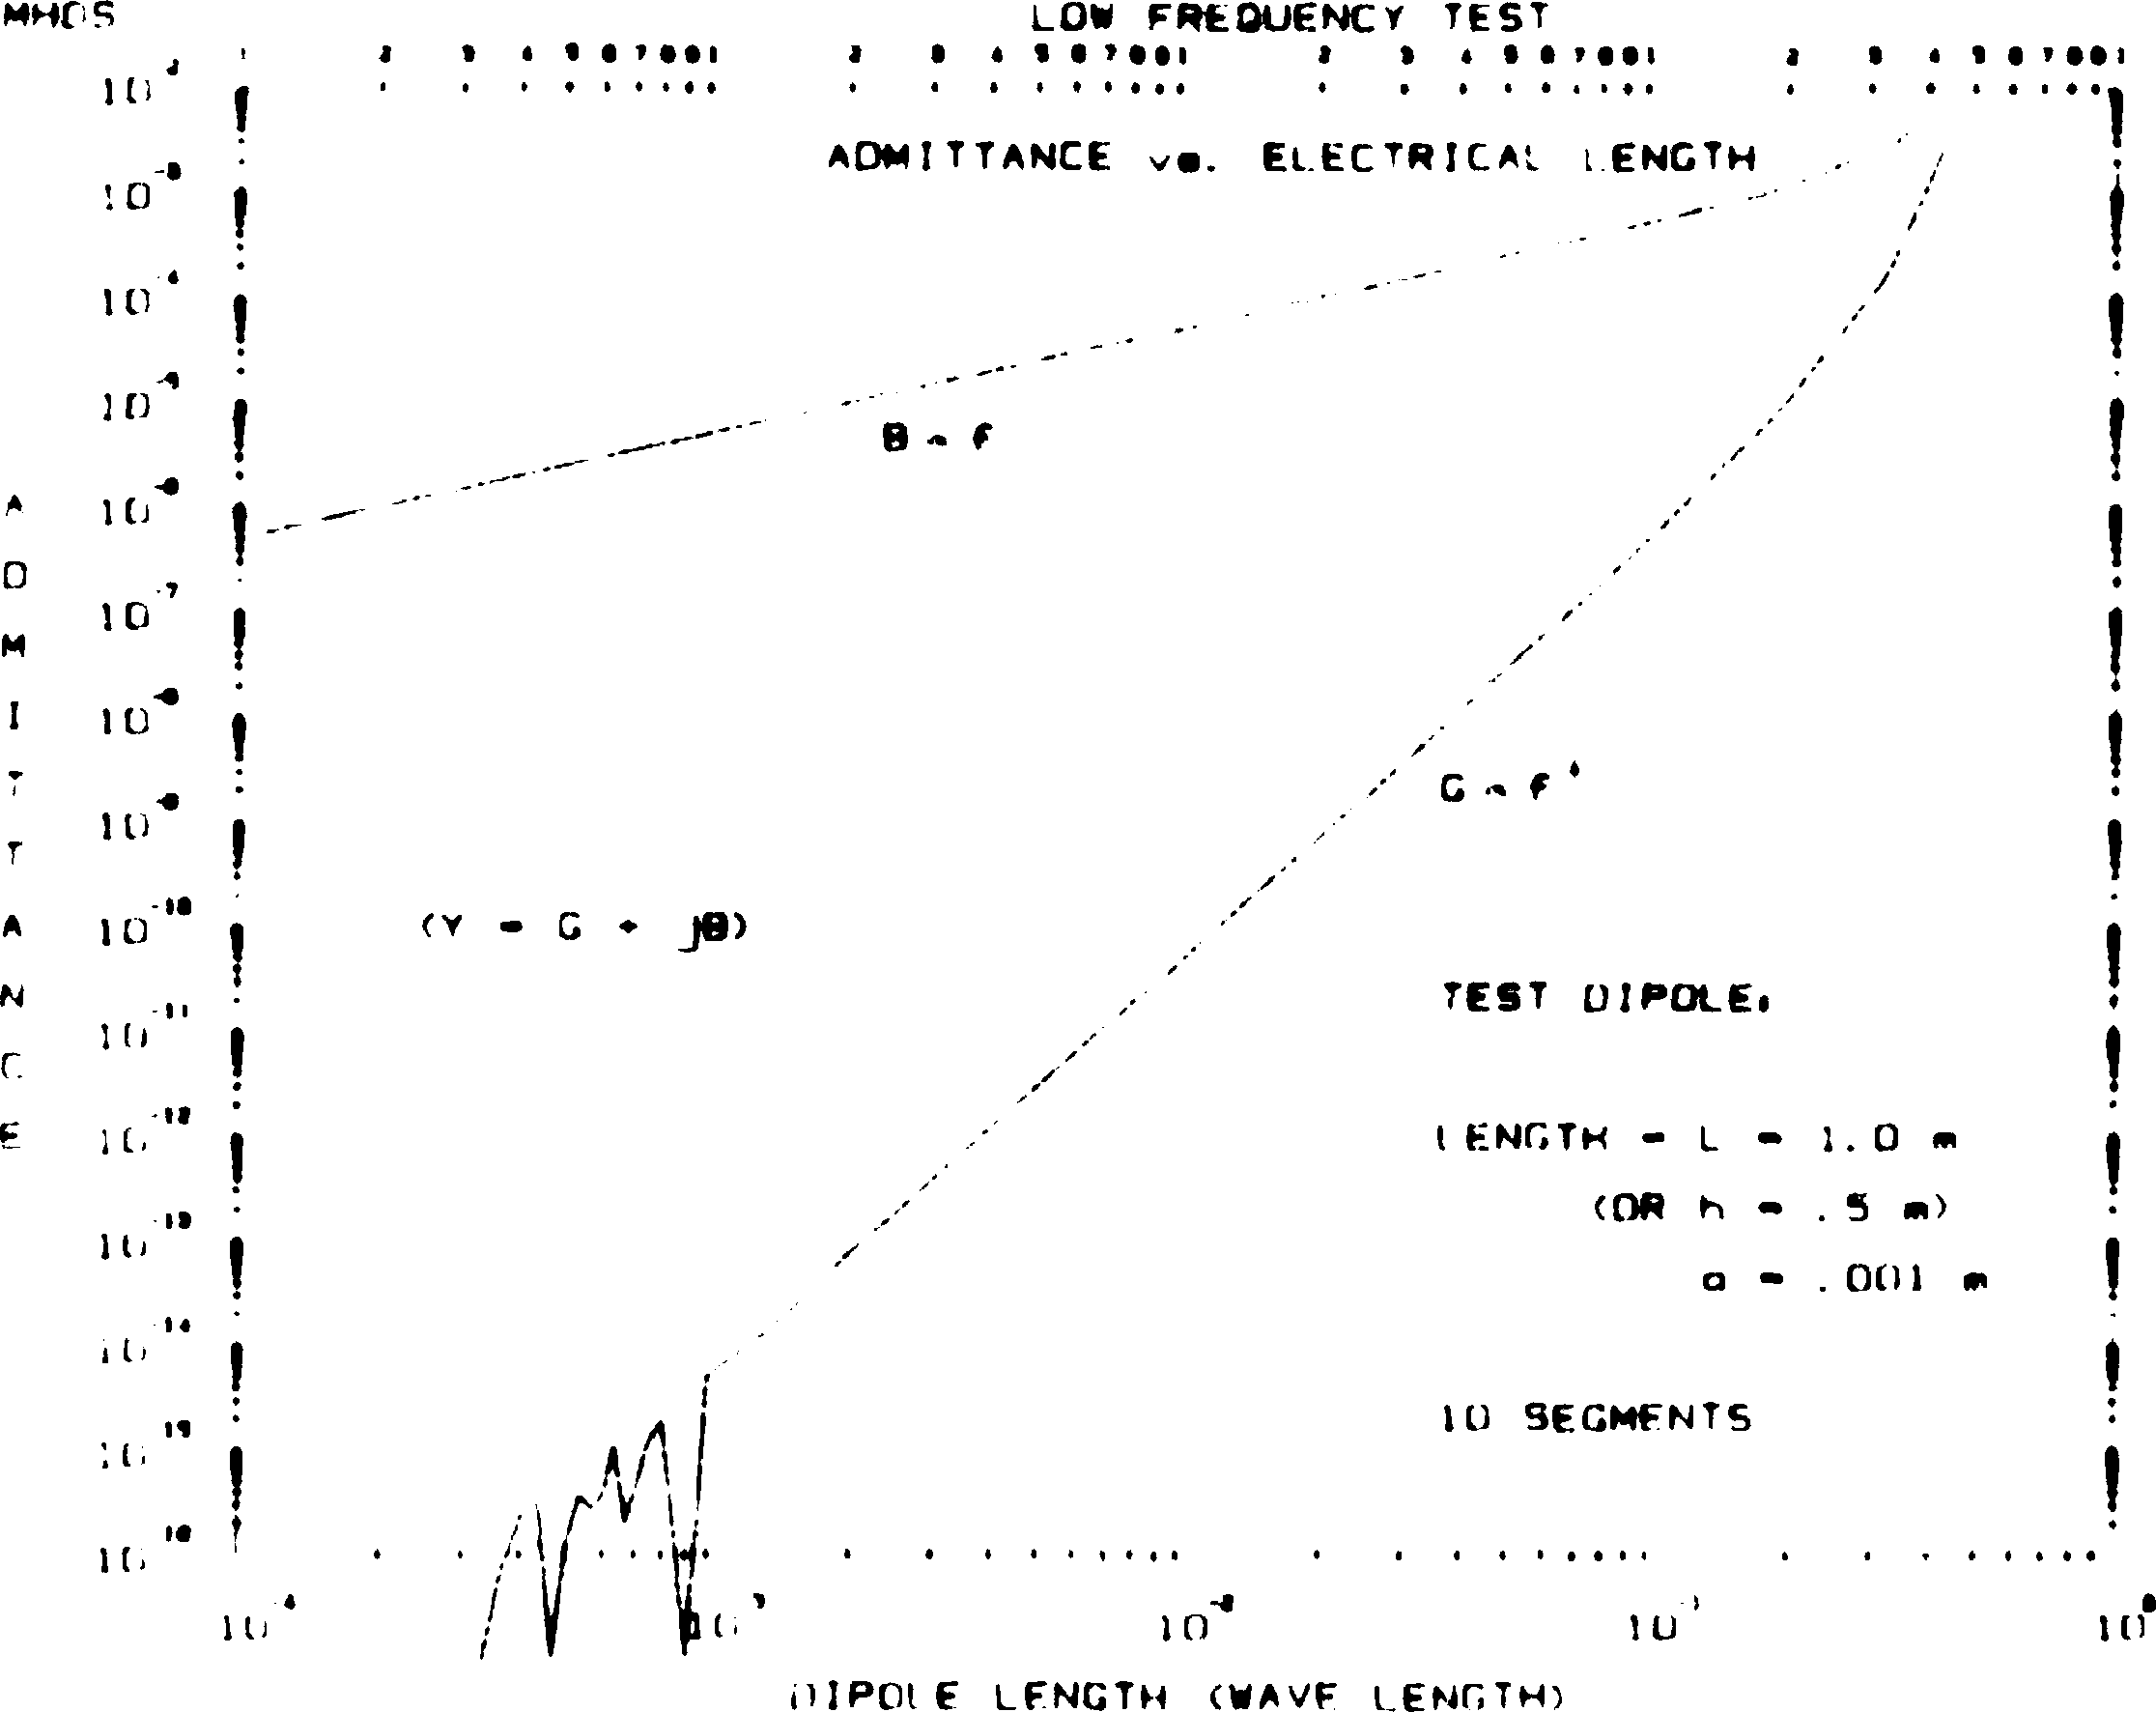
\includegraphics{fig14.eps}}
\caption{[Admittance vs. Dipole length] predicted by MININEC}
\label{fig14}
\end{sidewaysfigure}
\afterpage\clearpage

Reliable, accurate answers are obtained when the user has accumulated
sufficient experience from frequent and systematic exercise of the
program to recognize problem areas. He must be fully aware of potential
difficulties throughout the modeling process, from initially setting up
a problem to interpreting the results. It is recommended that the user
run MININEC for a number of elementary problems, comparing the results
to independent solutions or real world measurements, until he has the
confidence to apply the code to a problem for which the answer is
unknown. The examples in this section provide a good place to start.

Development of confidence in the computer solution is a process of
discovery of the limitations of the computer program. This entails the
modeling of a number of simple antenna structures found in standard
texts on antenna theory. The results may be used as guidelines to model
more complex antenna geometries. Natural first choices are dipoles in
free space and over ground (or monopoles), followed by TEE and inverted
L shaped antennas, etc. For each antenna type, a number of problems are
selected involving different wire lengths and radii. MININEC is run for
each antenna problem a number of times, varying segmentation (i.e., a
convergence test) and other parameters to reveal the program
limitations. Insight for effective application of the program is gained
from comparisons with measured data or analytical solutions (when
available). In this manner, modeling guidelines are derived and updated
from simpler antenna problems for which there is reliable measured data
or generally accepted theoretical data.

\subsection{Dipole Antennas}
The theoretical behavior of the dipole antenna has been studied
intensely, and the literature is rich with exammples that include
measured and theoretical data, \cite{r8},~\cite{r9},
\cite{r15},~\cite{r16}. Comparison of MININEC results to this data for
dipoles of various dimensions establishes validation and provides the
basis for modeling guidelines. For example, convergence tests for
various length dipoles reveals the accuracy that can be expected and
provides a rational criterion for selection of segmentation density (the
number of segments per wire) based on wire length in wave lengths.

Figure~\ref{fig6} through \ref{fig11} show the results of convergence
tests for an electrically short dipole (much shorter than the first
resonance length), a dipole near resonance, and a dipole near
antiresonance, respectively. Each dipole is electrically thin and center
driven. Part (a) Figures (\ref{fig6},~\ref{fig8}, and~\ref{fig10}) give
the variation of admittance, versus the number of segments. Part (b)
Figures (\ref{fig7},~\ref{fig9}, and~\ref{fig11}) give the percent
difference between MININEC and the values published by R.W.P. King,
\cite{r8}, \cite{r9}.

The electrically short dipole, Figures~\ref{fig6} and~\ref{fig7}, and
the half wave dipole, Figures~\ref{fig8} and~\ref{fig9}, show definitive
signs of convergence and stability. No sign of convergence is seen for
the antiresonant dipole, Figure~\ref{fig10} and~\ref{fig11}. The authors
also have seen similar convergence problems near antiresonance for other
method of moment codes (notably NEC). Figures~\ref{fig6}
through~\ref{fig11} can be used as guidance for selection of the
segmentation density. An antenna is modeled as a collection of wires.
Each wire is divided into a number of short segments selected by the
user. The number of segments to achieve a desirable confidence level can
be based on the results of Figures~\ref{fig6} through~\ref{fig11},
depending on the wire length in wave lengths. Using this data does not
guarantee convergence or the percent accuracy for a more complicated
antenna, but it does provide a starting point. Convergence testing is
always advisable.

Given the convergence properties of MININEC, how well does it predict
dipole properties? Figure~\ref{fig12} is a comparison of a single,
30-segment MININEC model to the theory given by King
\cite{r9}. Shown is the admittance-versus-dipole length for
both MININEC and King. The difference is less that .5 millimho for most
of the range, with the greatest difference of about 1.5 millimhos in the
susceptance at a dipole length of .64 wave lengths. For longer or
shorter antennas, the user is advised to perform suitable convergence
tests.

The accuracy of the method of moments solution depends also on meeting
the thin wire criterion. To illustrate, Figure~\ref{fig13} shows the
variation of admittance versus the wire radius. The data given by King
\cite{r9} are slso shown for radii betwenn $10^{-3}$ and
$10^{-2}$ wave lengths. The segment to radius ratio, $\Delta/a$, is 25
at $10^{-3}$ and 2.5 at $10^{-2}$. For thicker wires than $10^{-2}$, the
thin wire criteria is not achieved and the results are expected to be
not as good. The data show valid behavior for thin wires with
$\Delta/a > 2.5$ or radii of $10^{-2}$ wave lengths and smaller.

Numerical problems may occur in the solution when quantities become too
small for the inherent accuracy of the computer. An example is the
erroneous results that can occur for very short segments.
Figure~\ref{fig14} shows the results of a test designed to identify the
short segment limit. Shown is the admittance-versus-dipole length in wave
lengths for a 10-segment dipole in free space. The conductance and
susceptance displays the proper behavior for a dipole length greater
than $10^{-3}$ wave lengths. This corresponds to a segment length of
$10^{-4}$ wave lengths and longer. Below $10^{-3}$, the conductance
oscillates about the expected values as the segment length is reduced,
and at times displays negative, non-physical values. A change from
single precision to double precision extends the validity range to even
shorter segments, but significantly increases the solution time beyond
acceptable run times for a 16-bit microcomputer. For MININEC, on a
16-bit machine in single precision, the segment length should always be
greater than $10^{-4}$ wave lengths.

\begin{figure}[t]
\centerline{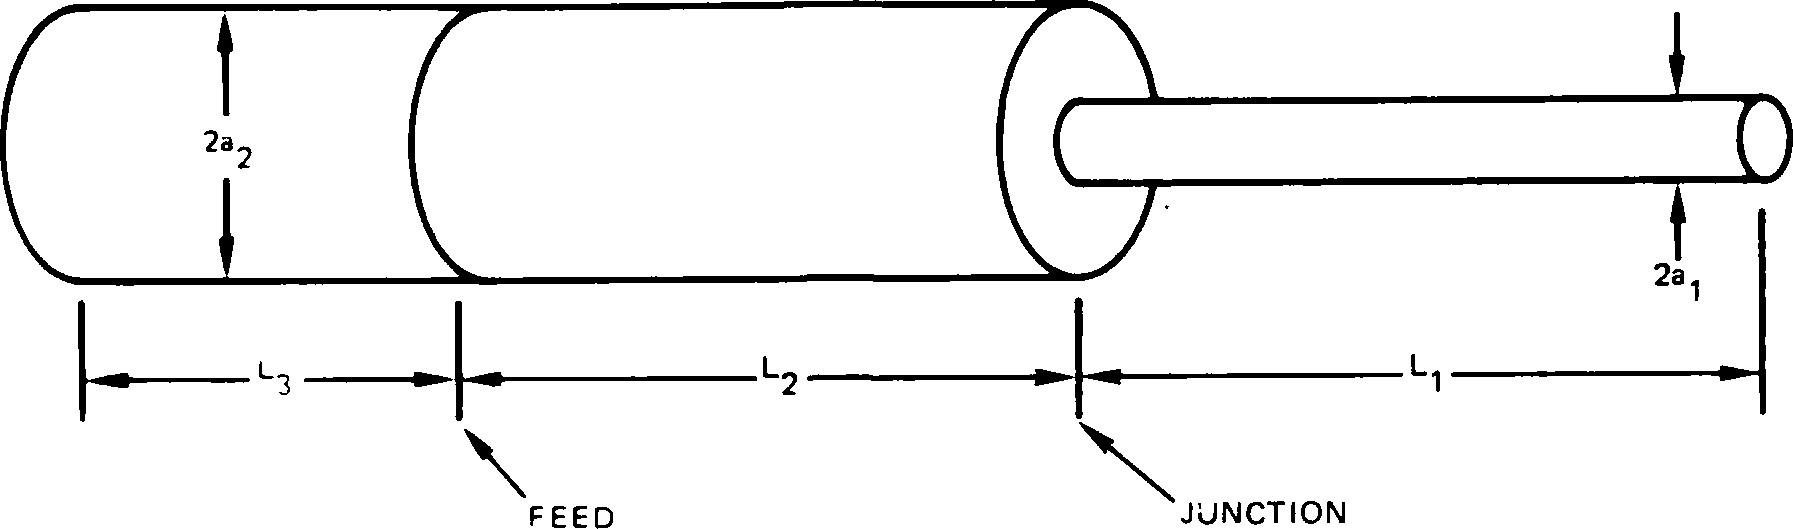
\includegraphics{fig15.eps}}
\caption{Geometry for the stepped radius antenna problem}
\label{fig15}
\end{figure}

Antennas are often constructed of wires and towers or other conductors
with vastly different radii. Even simple dipoles may have tapered
elements. A typical MININEC model may therefore involve the connection
of wires with large step changes in radii. The stepped-radius wire
junction has been extensively studied by Glisson and Wilton
\cite{r17}. Figure~\ref{fig15} is the stepped wire geometry
used in their study. They adapted a body of revolution computer code,
PEC; to solve very accurately for currents and charges along the stepped
wire antenna. The results were compared to NEC in this study.

\begin{sidewaysfigure}[htb]
\centerline{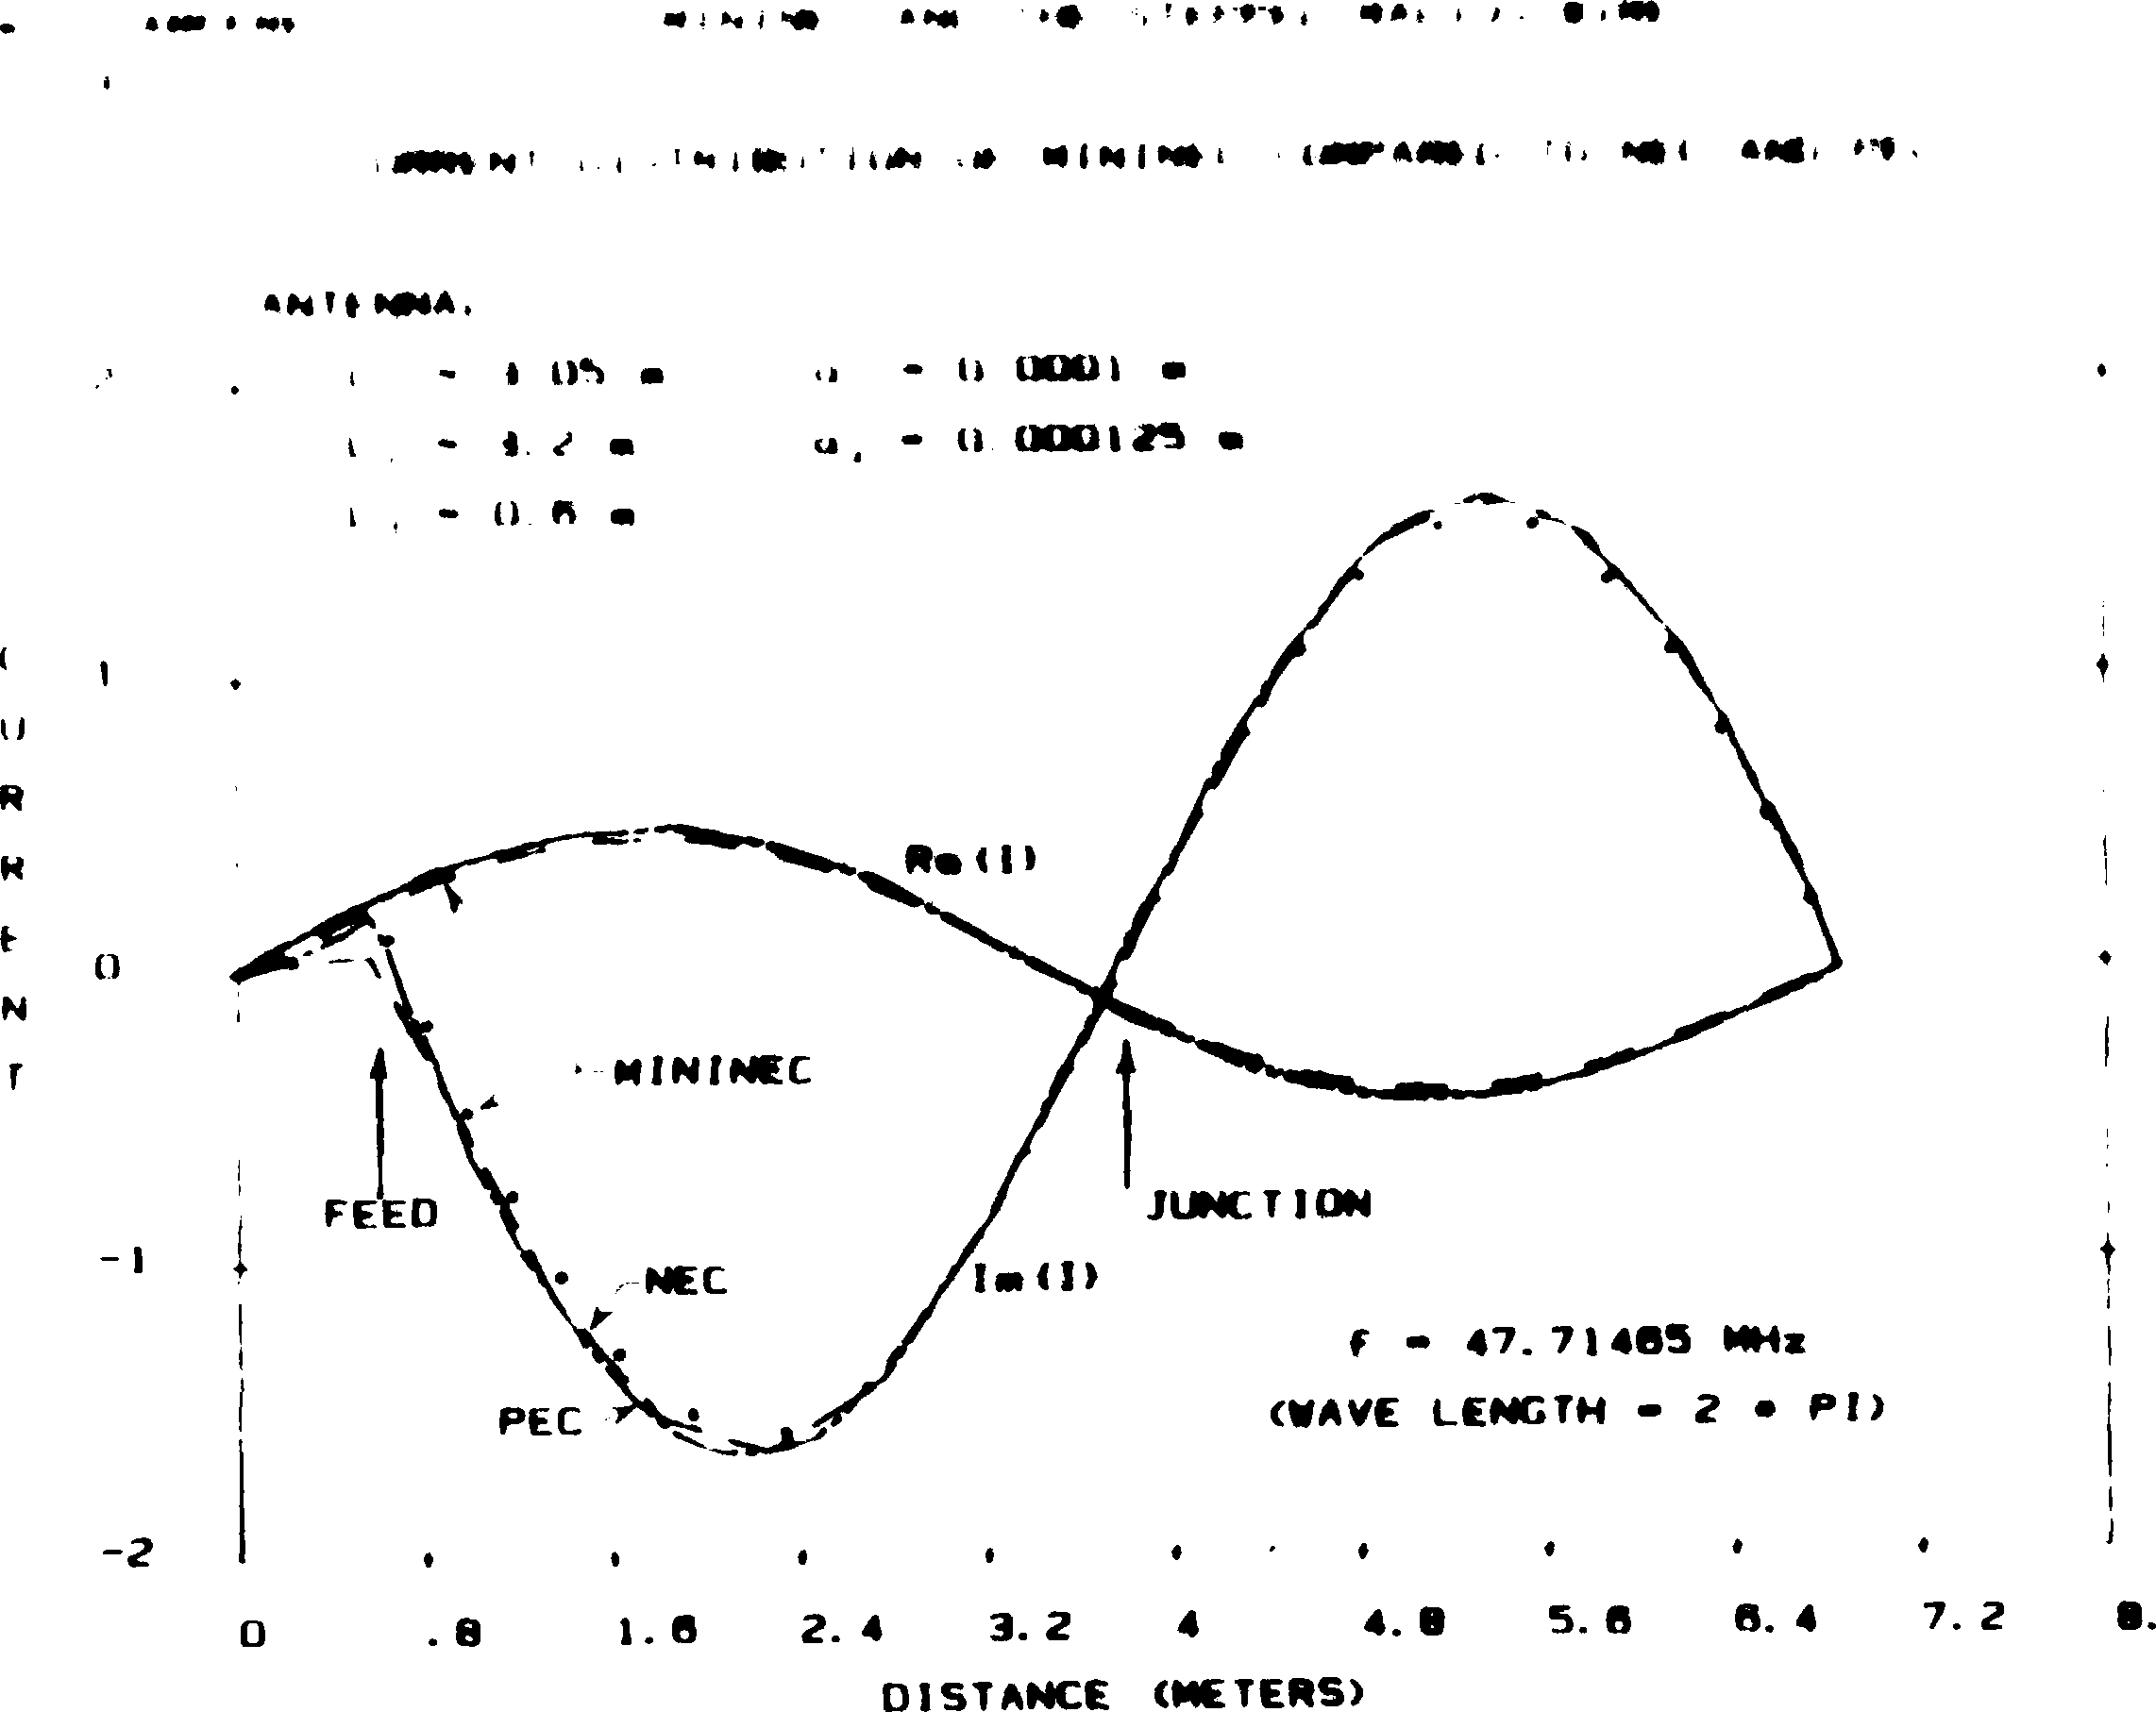
\includegraphics{fig16.eps}}
\caption{Currents for a stepped radius junction of $a_2/a_1 = 1.25$}
\label{fig16}
\end{sidewaysfigure}

\begin{sidewaysfigure}[htb]
\centerline{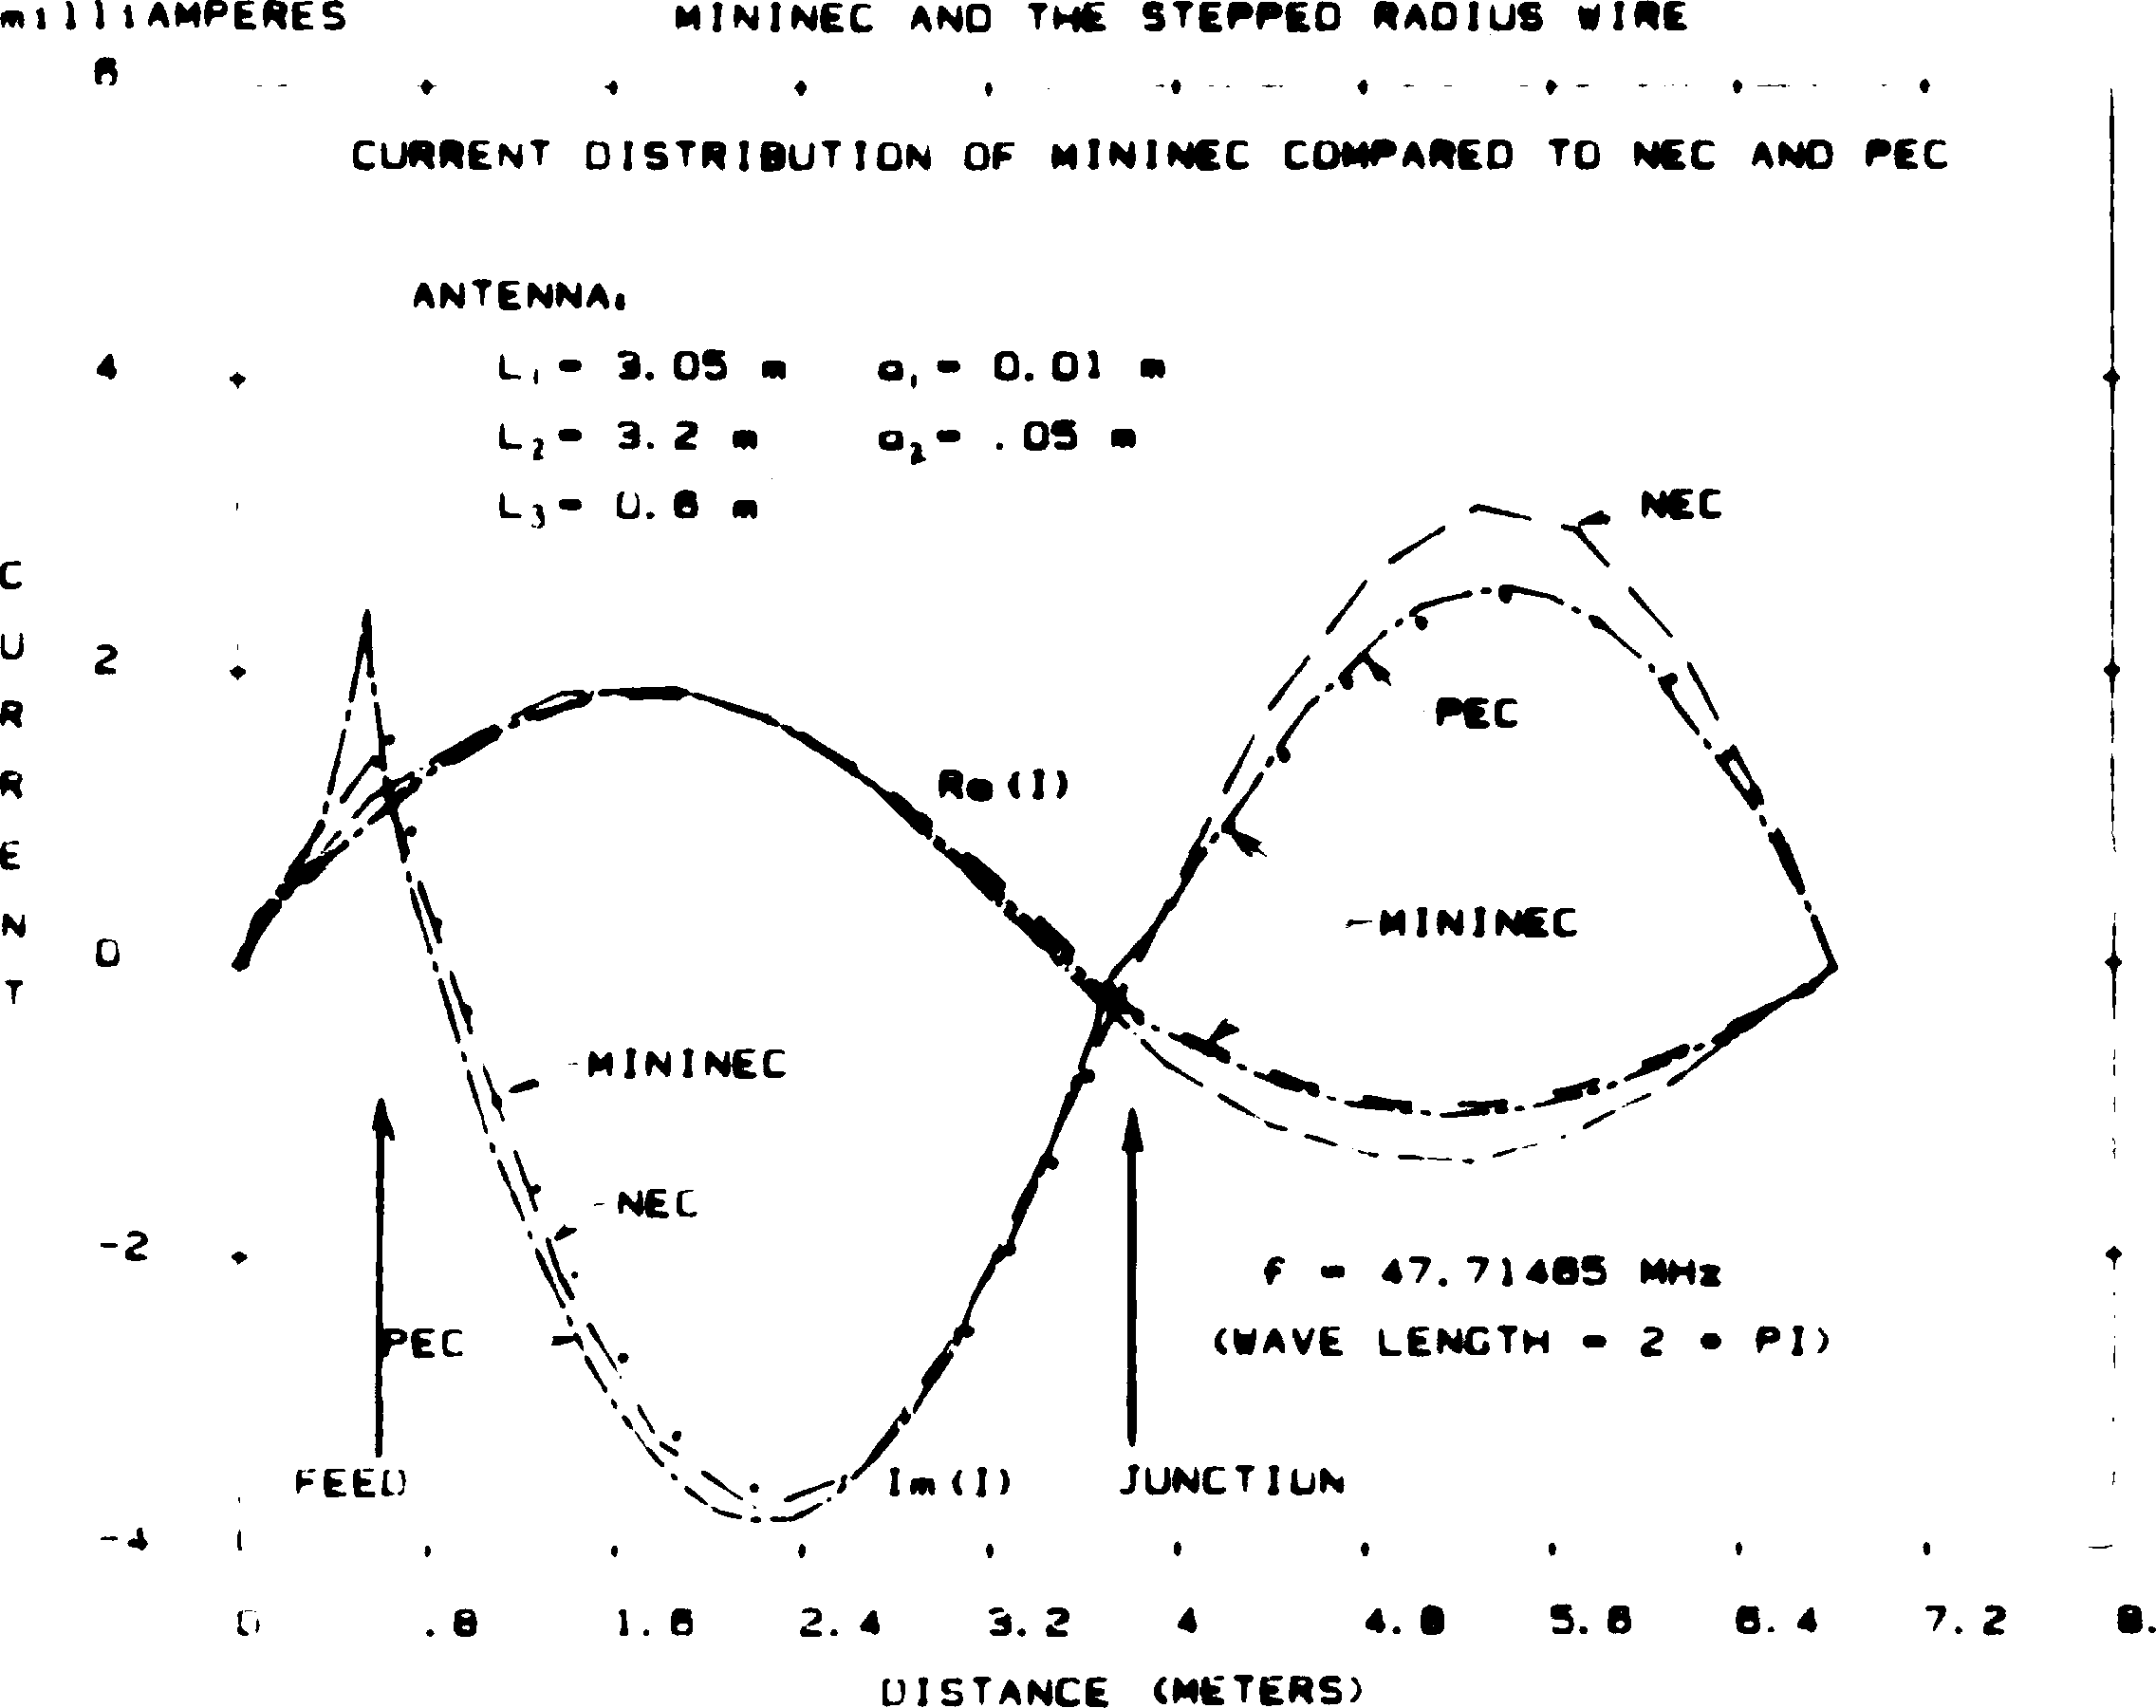
\includegraphics{fig17.eps}}
\caption{Currents for a stepped radius junction of $a_2/a_1 = 5$}
\label{fig17}
\end{sidewaysfigure}

\begin{sidewaysfigure}[htb]
\centerline{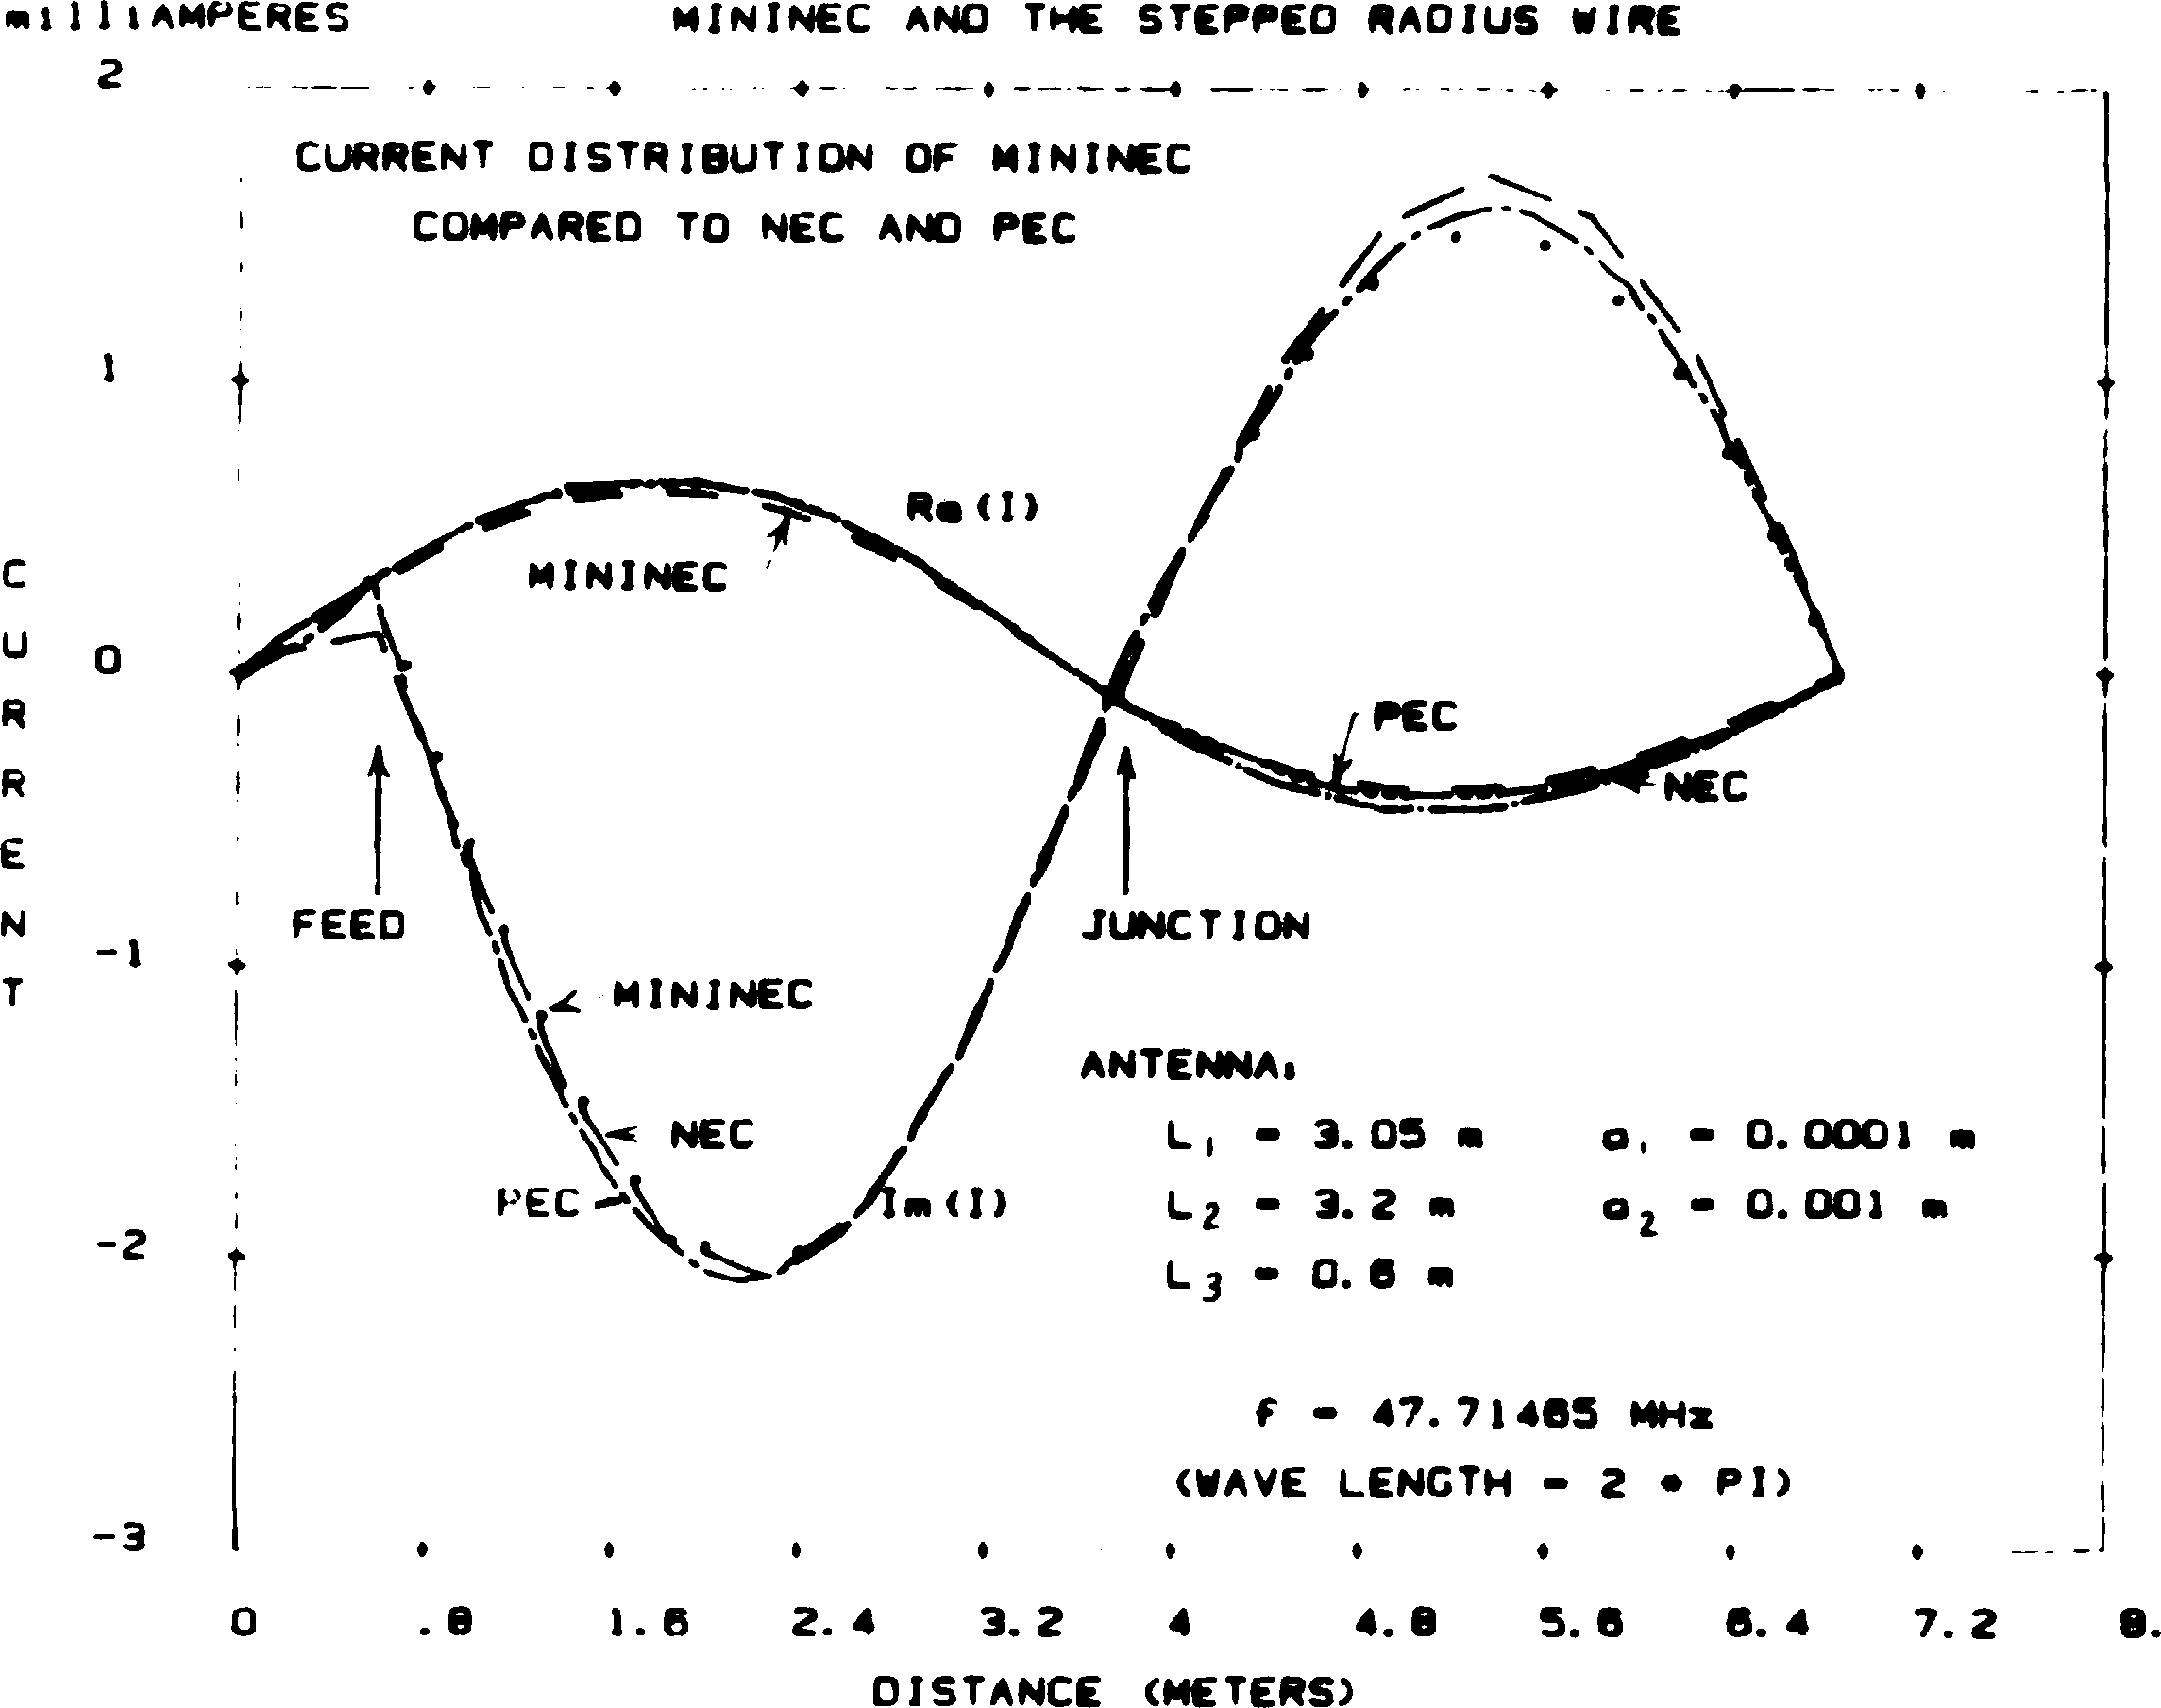
\includegraphics{fig18.eps}}
\caption{Currents for a stepped radius junction of $a_2/a_1 = 10$}
\label{fig18}
\end{sidewaysfigure}

\begin{sidewaysfigure}[htb]
\centerline{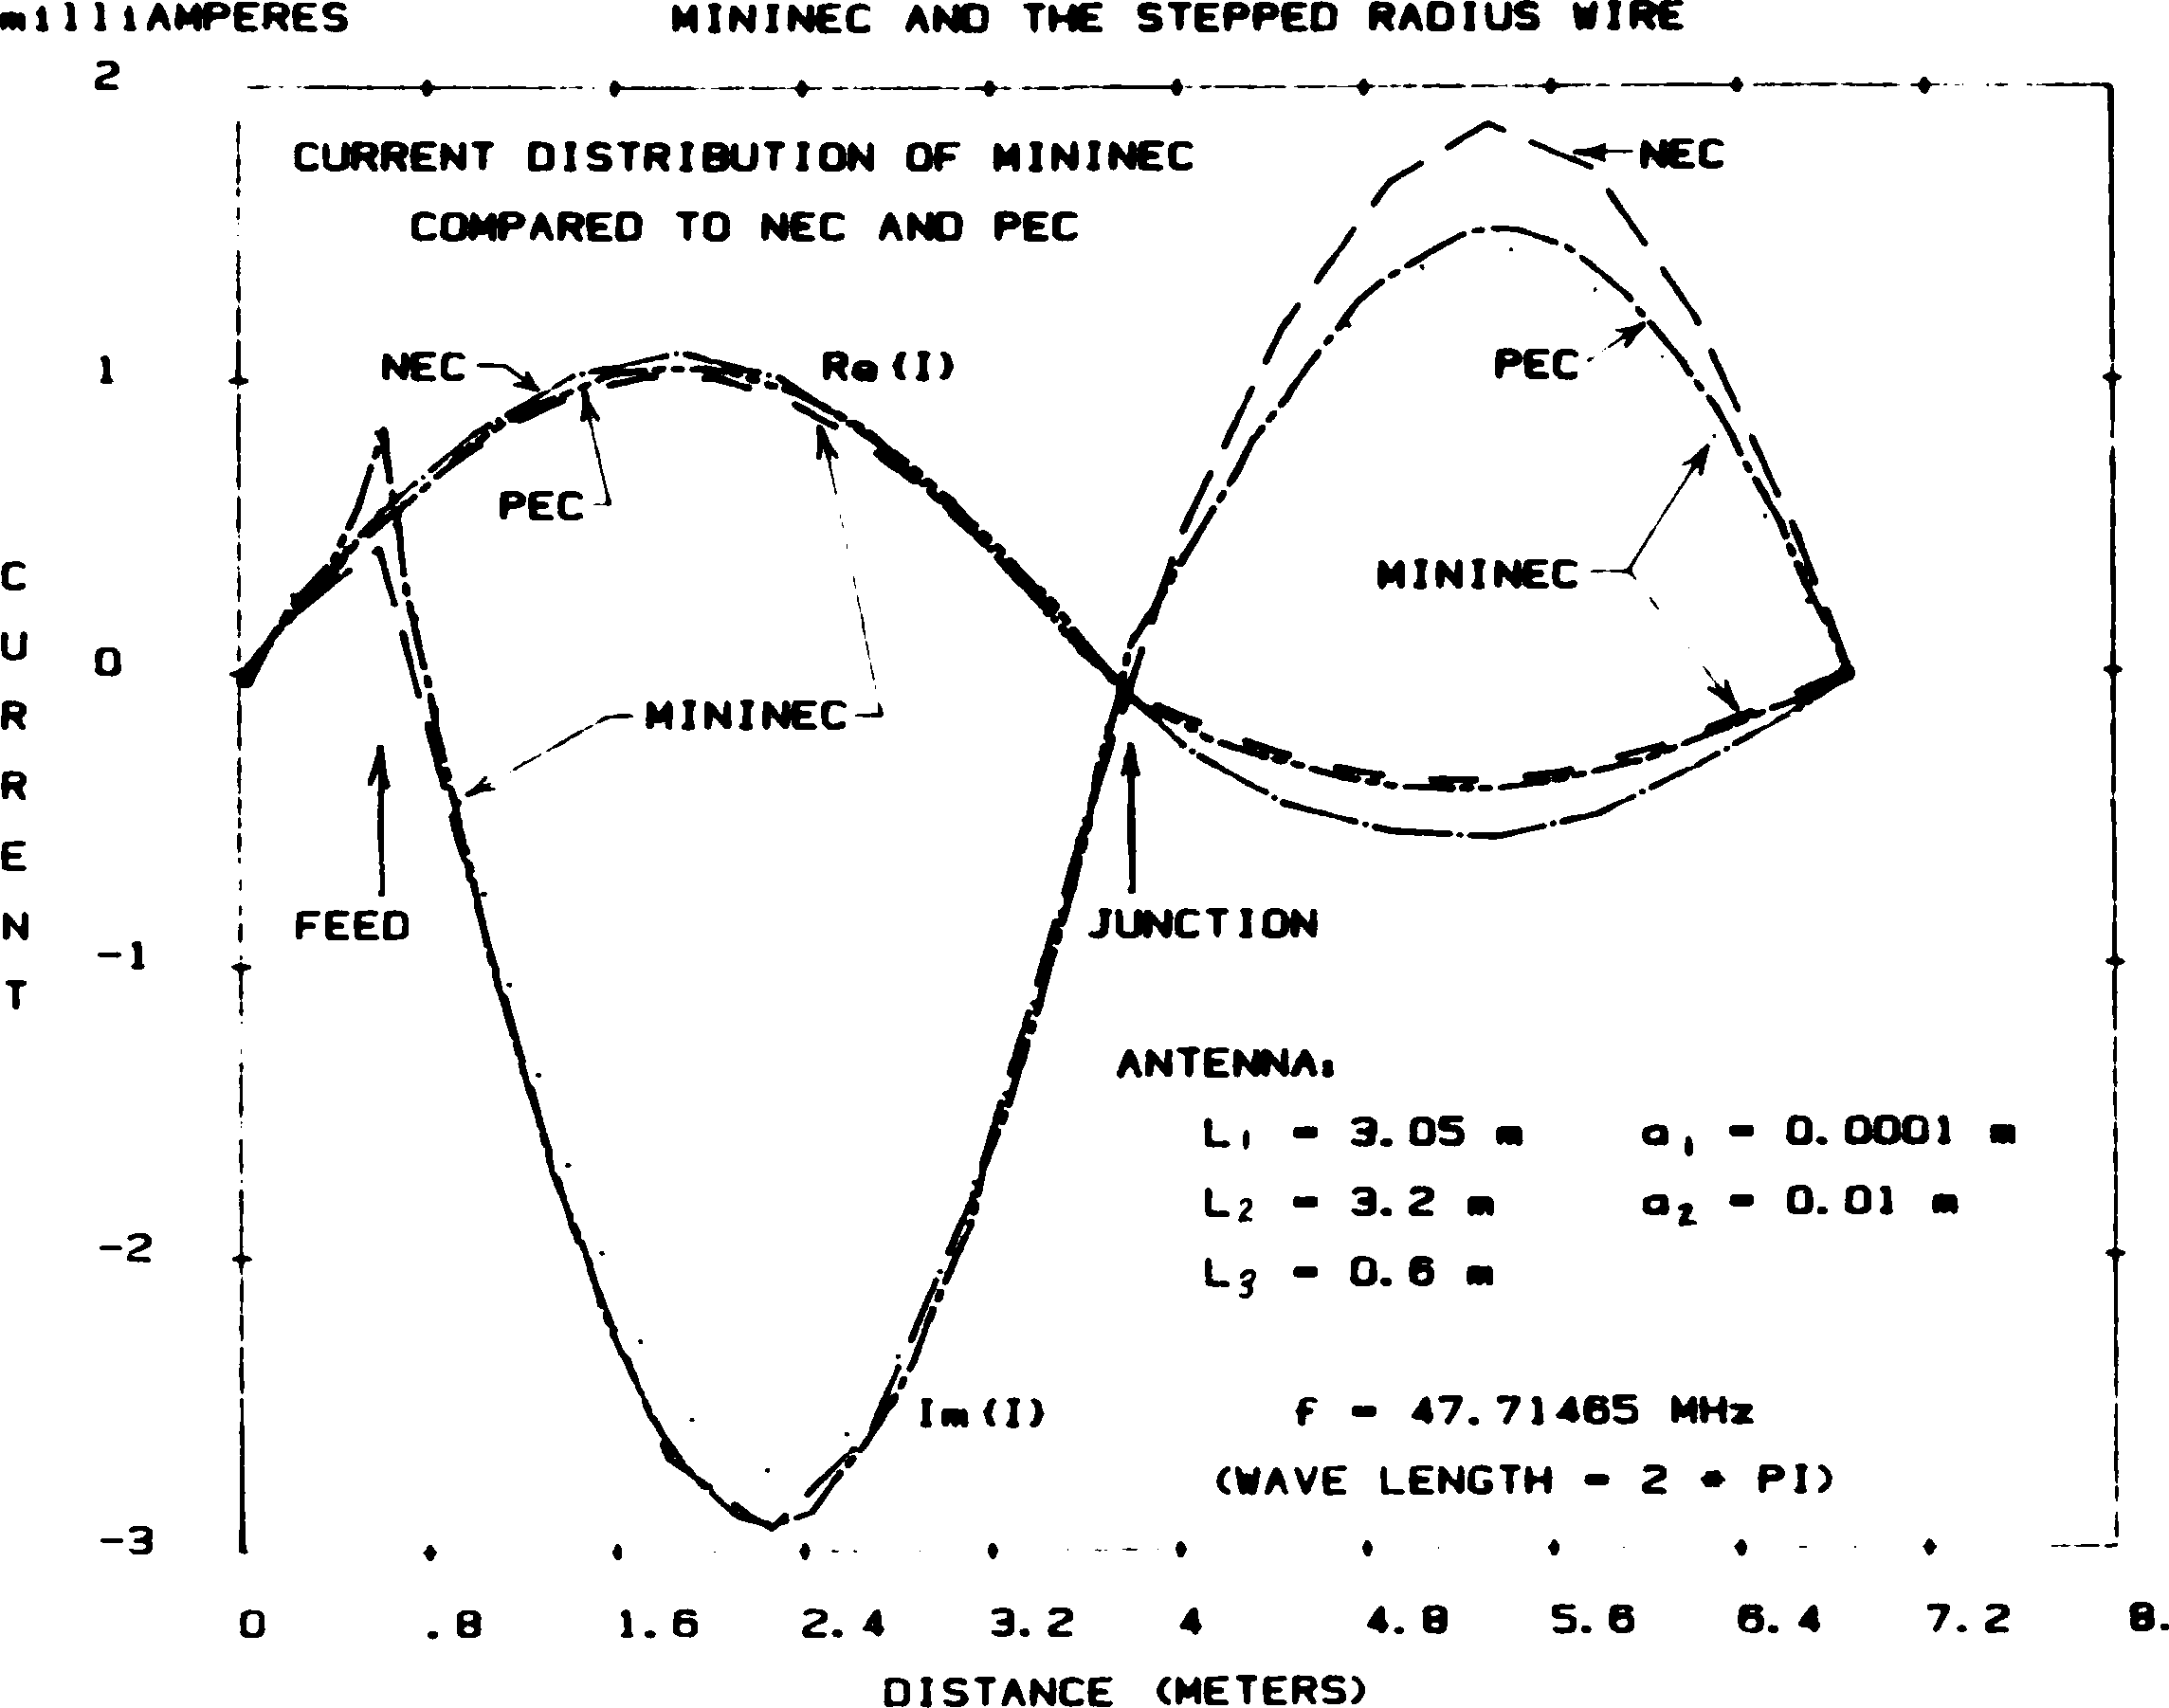
\includegraphics{fig19.eps}}
\caption{Currents for a stepped radius junction of $a_2/a_1 = 100$}
\label{fig19}
\end{sidewaysfigure}

\begin{sidewaysfigure}[htb]
\centerline{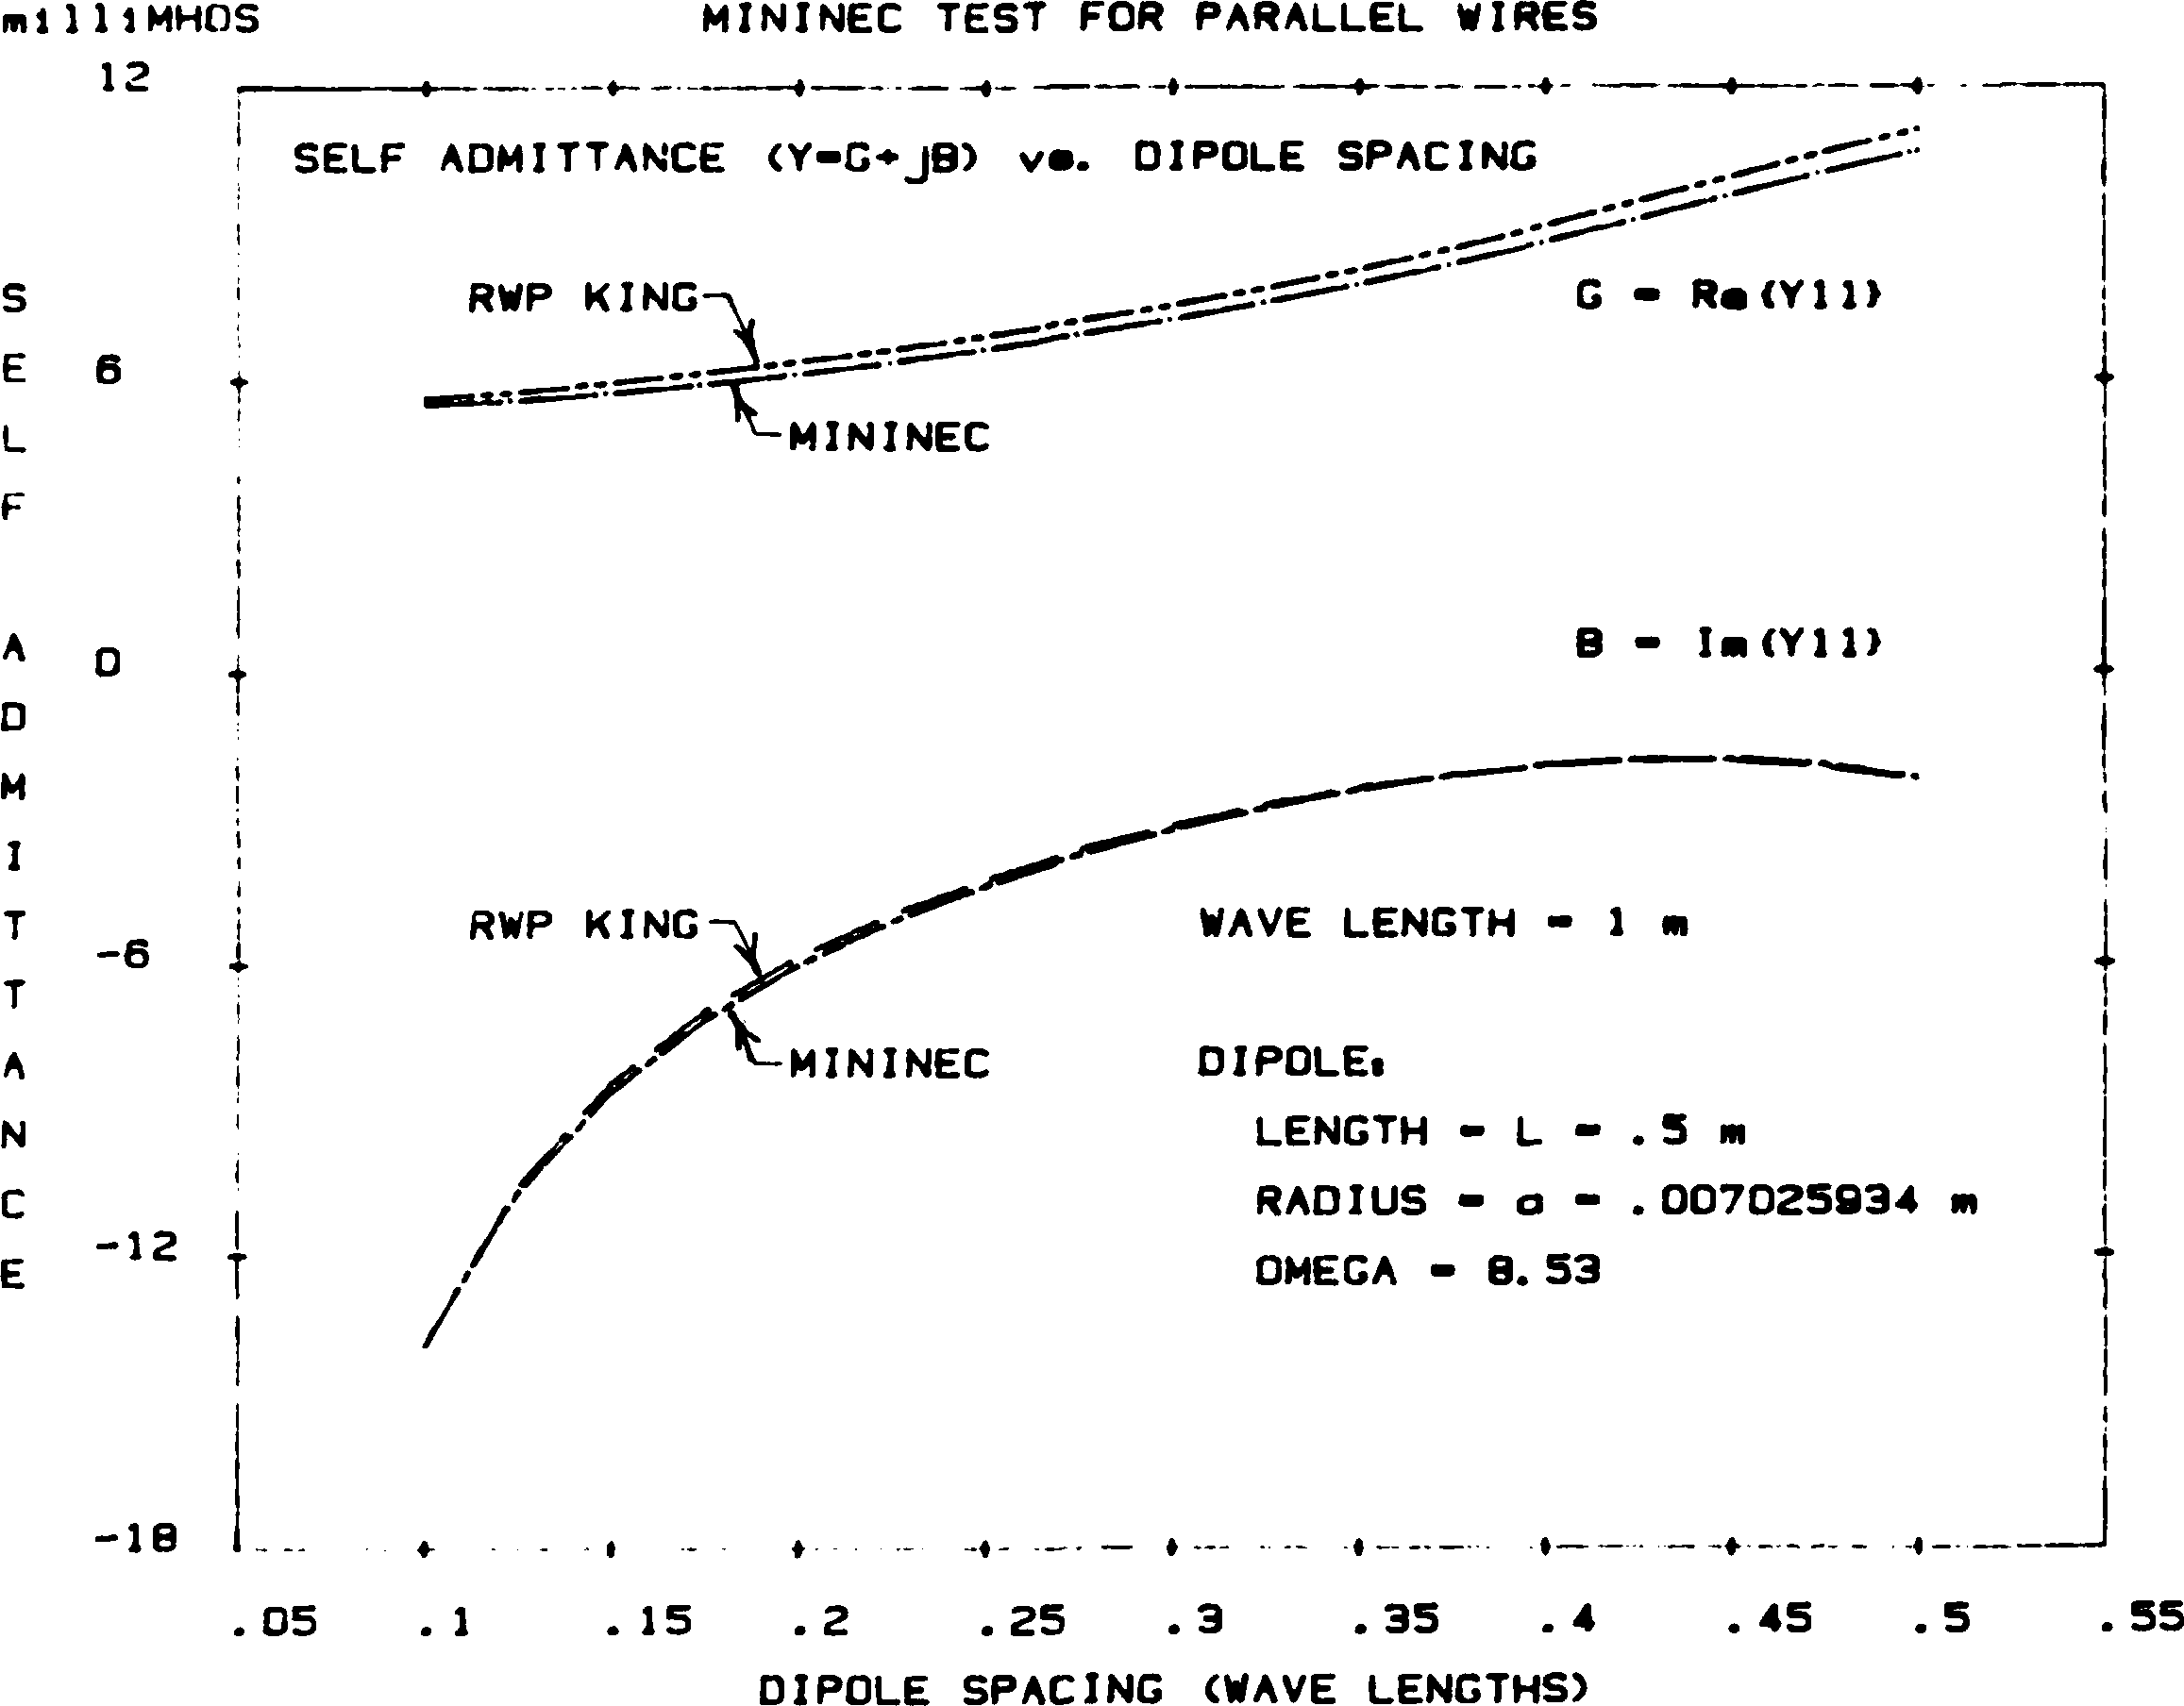
\includegraphics{fig20.eps}}
\caption{Self admittance computed by MININEC compared to the theory by
R. W. P. King for two parallel dipoles}
\label{fig20}
\end{sidewaysfigure}

\begin{sidewaysfigure}[htb]
\centerline{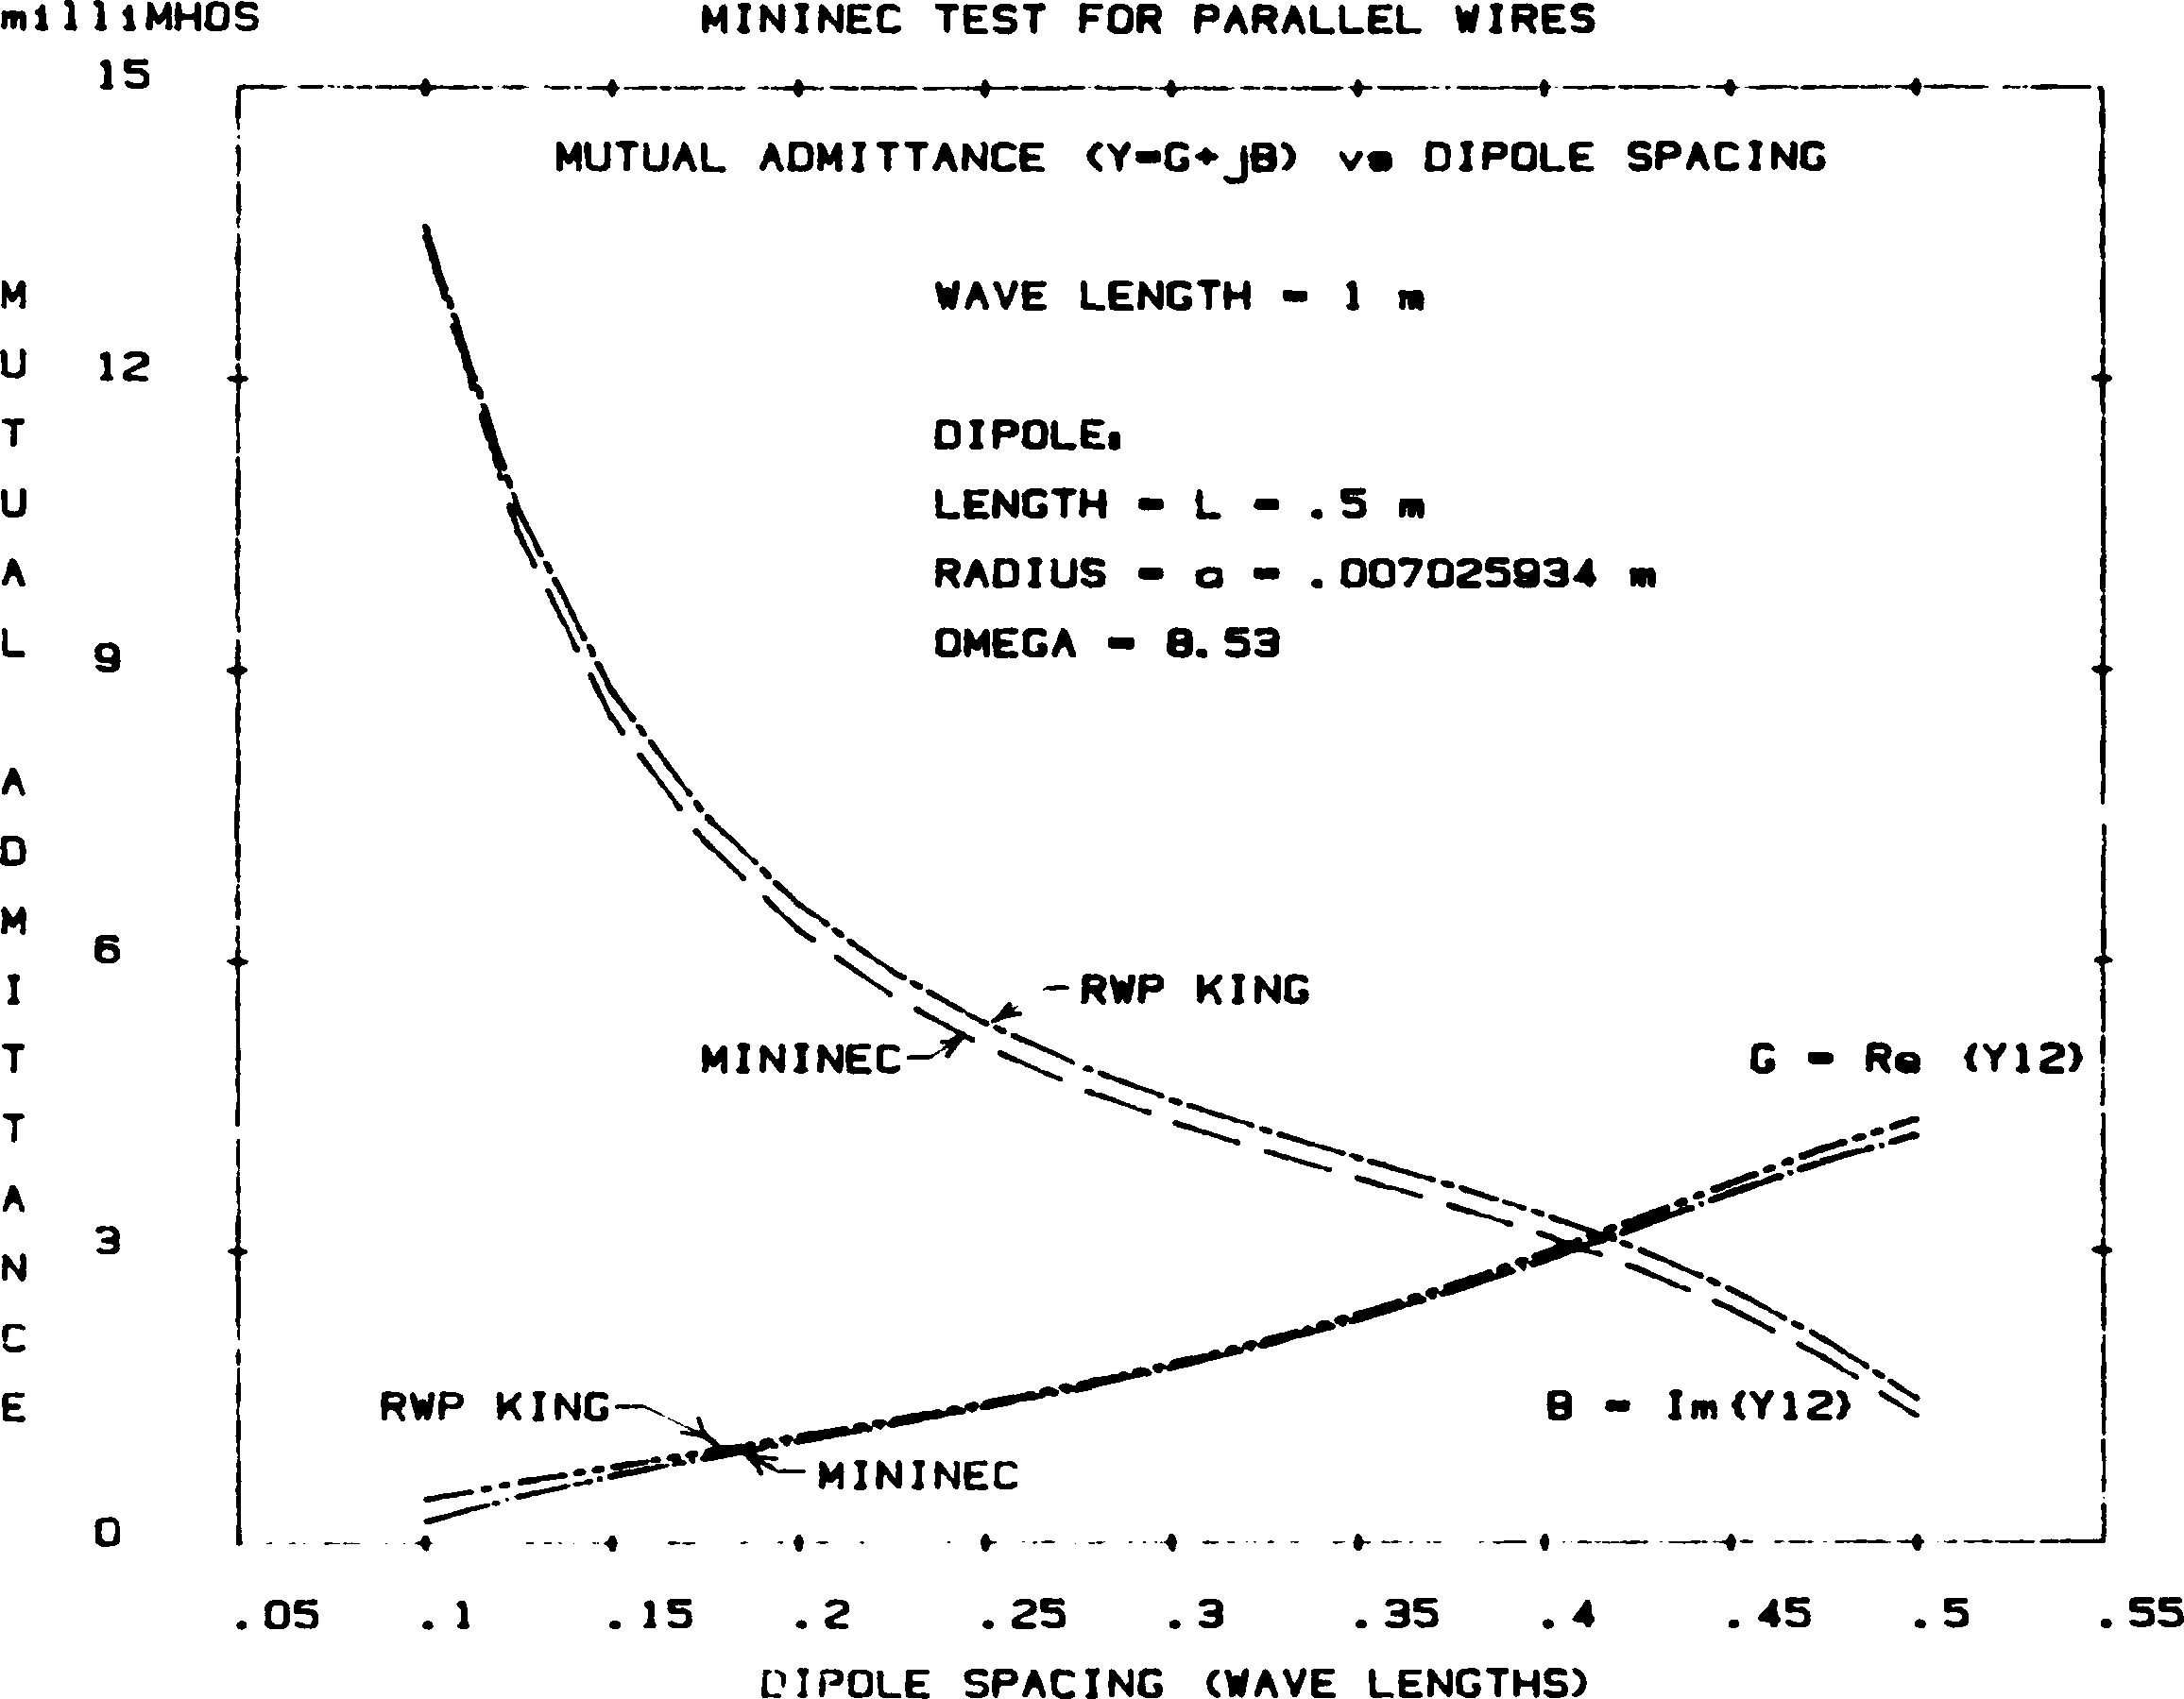
\includegraphics{fig21.eps}}
\caption{Mutual admittance computed by MININEC compared to the theory by
R. W. P. King for two parallel dipoles}
\label{fig21}
\end{sidewaysfigure}

\begin{sidewaysfigure}[htb]
\centerline{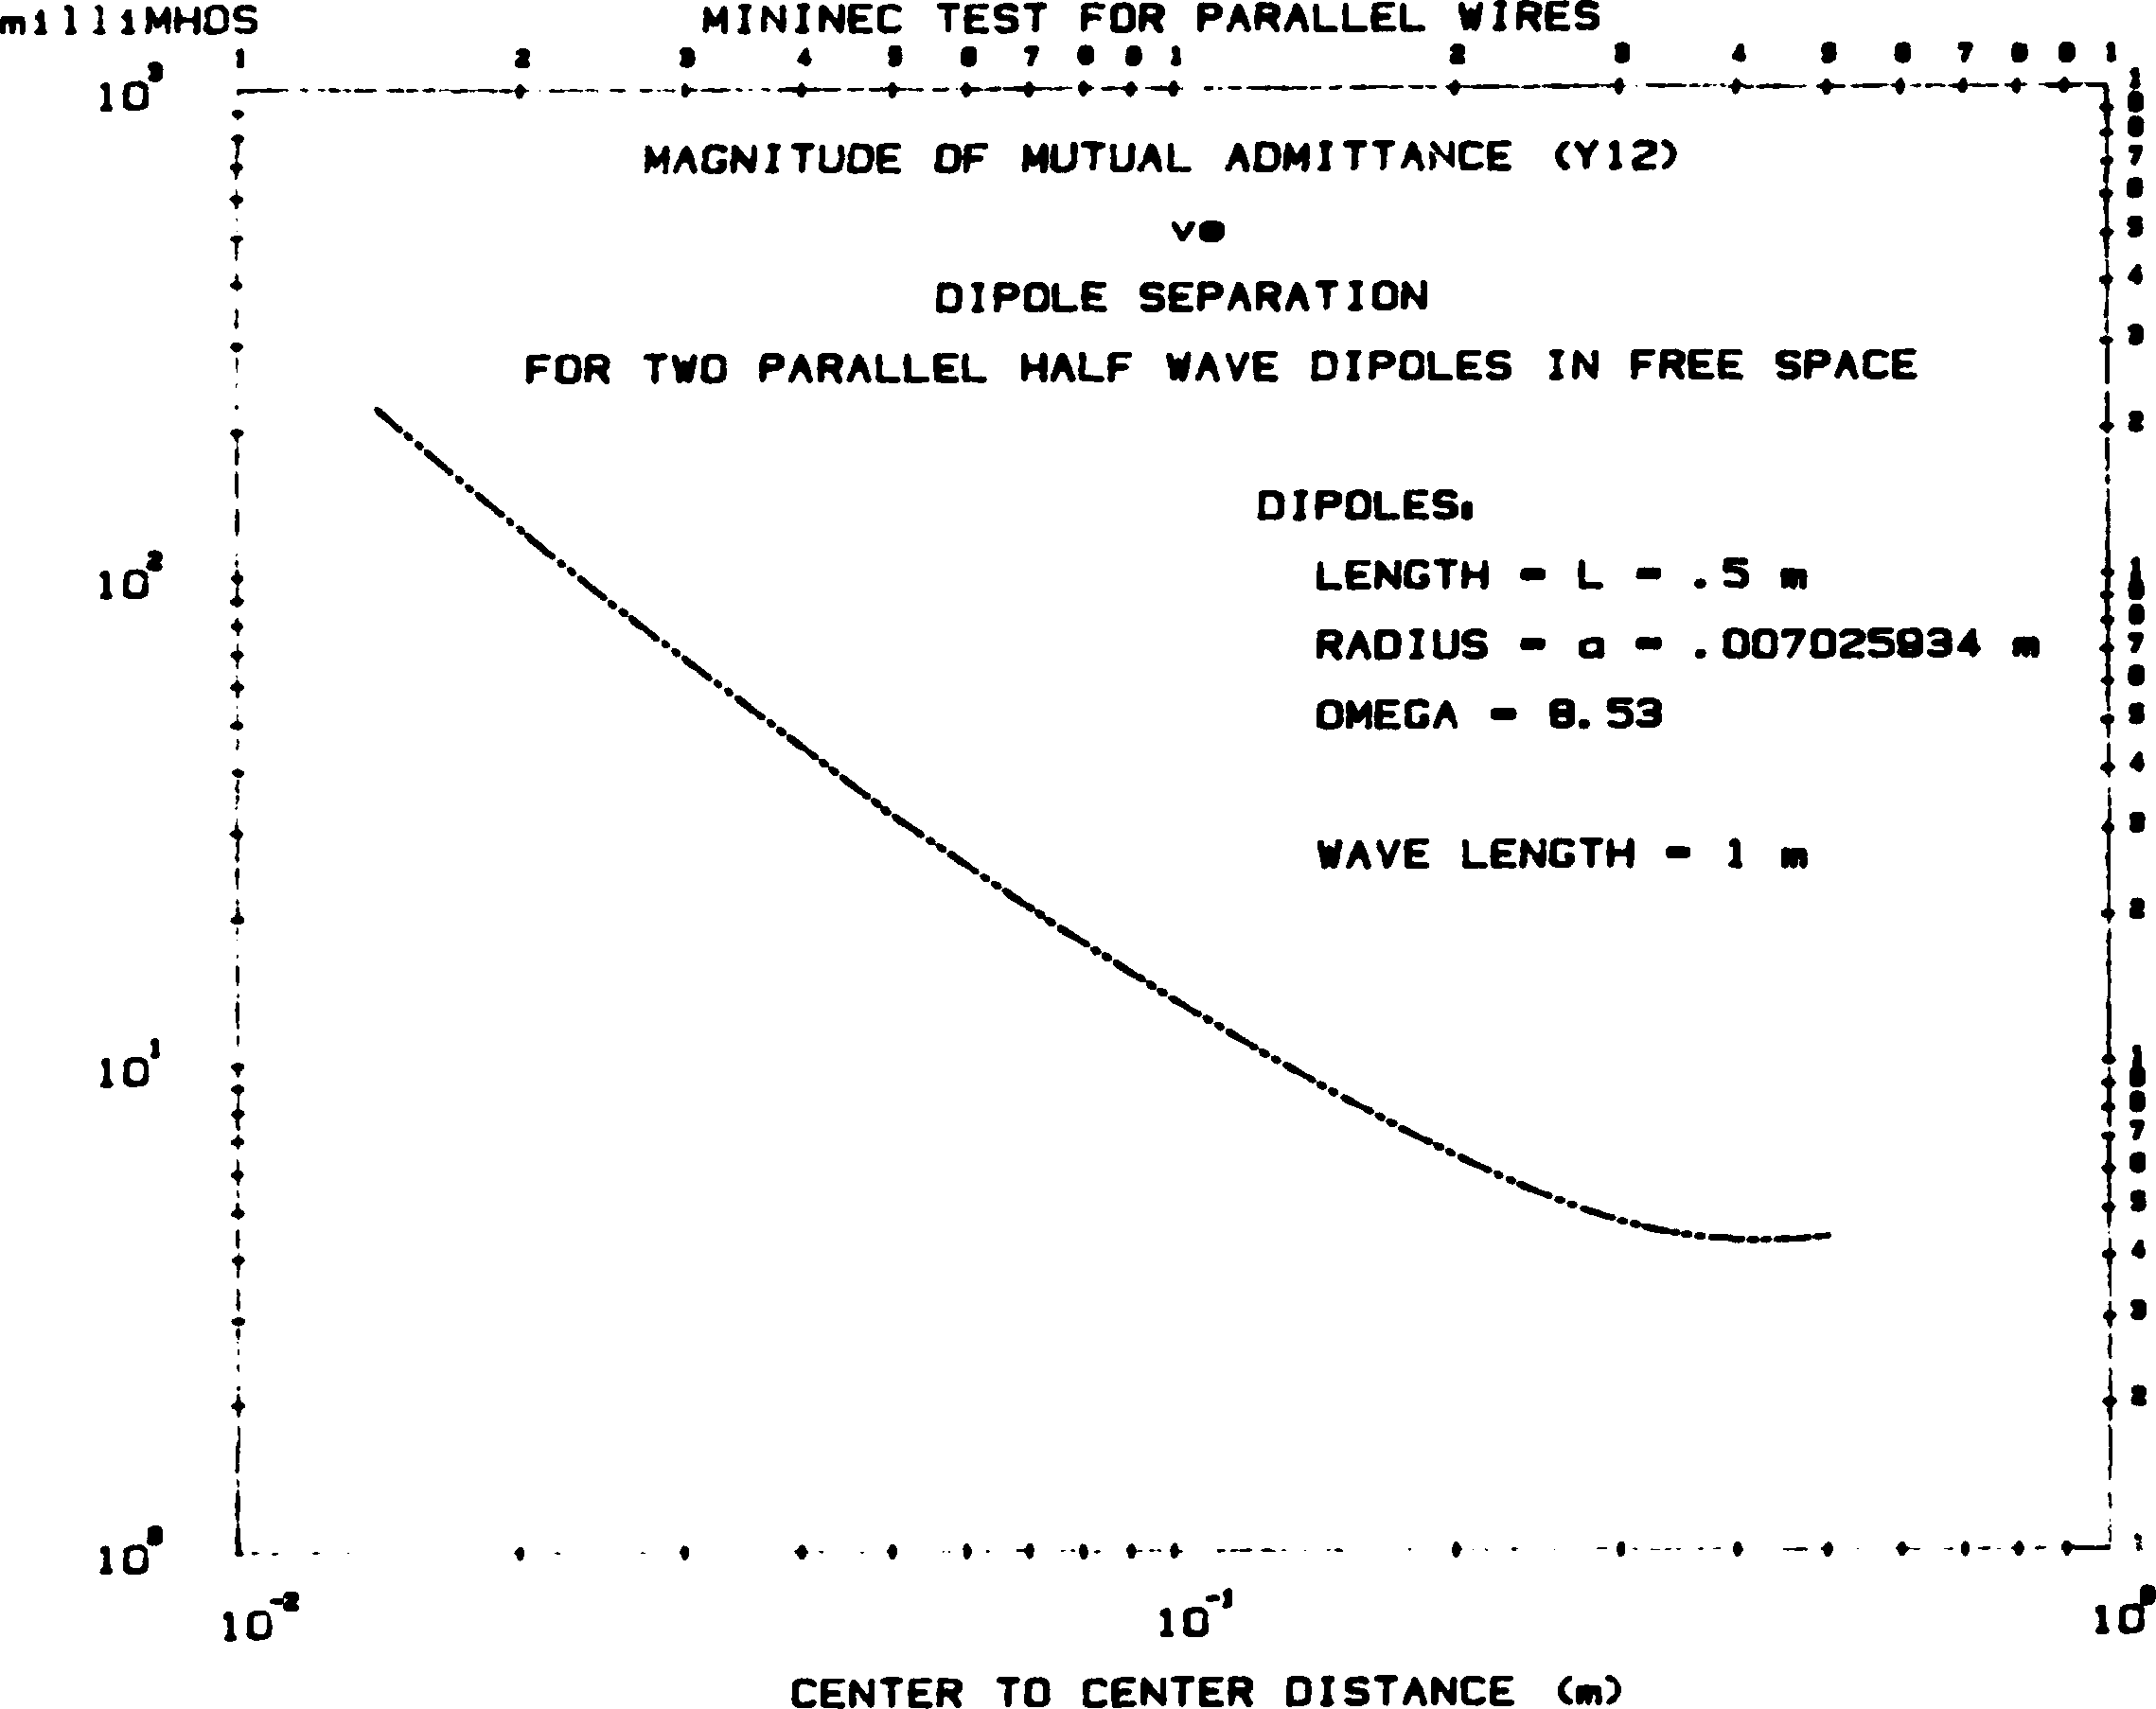
\includegraphics{fig22.eps}}
\caption{Magnitude of the mutual admittance between closely spaced
parallel dipoles}
\label{fig22}
\end{sidewaysfigure}

\begin{sidewaysfigure}[htb]
\centerline{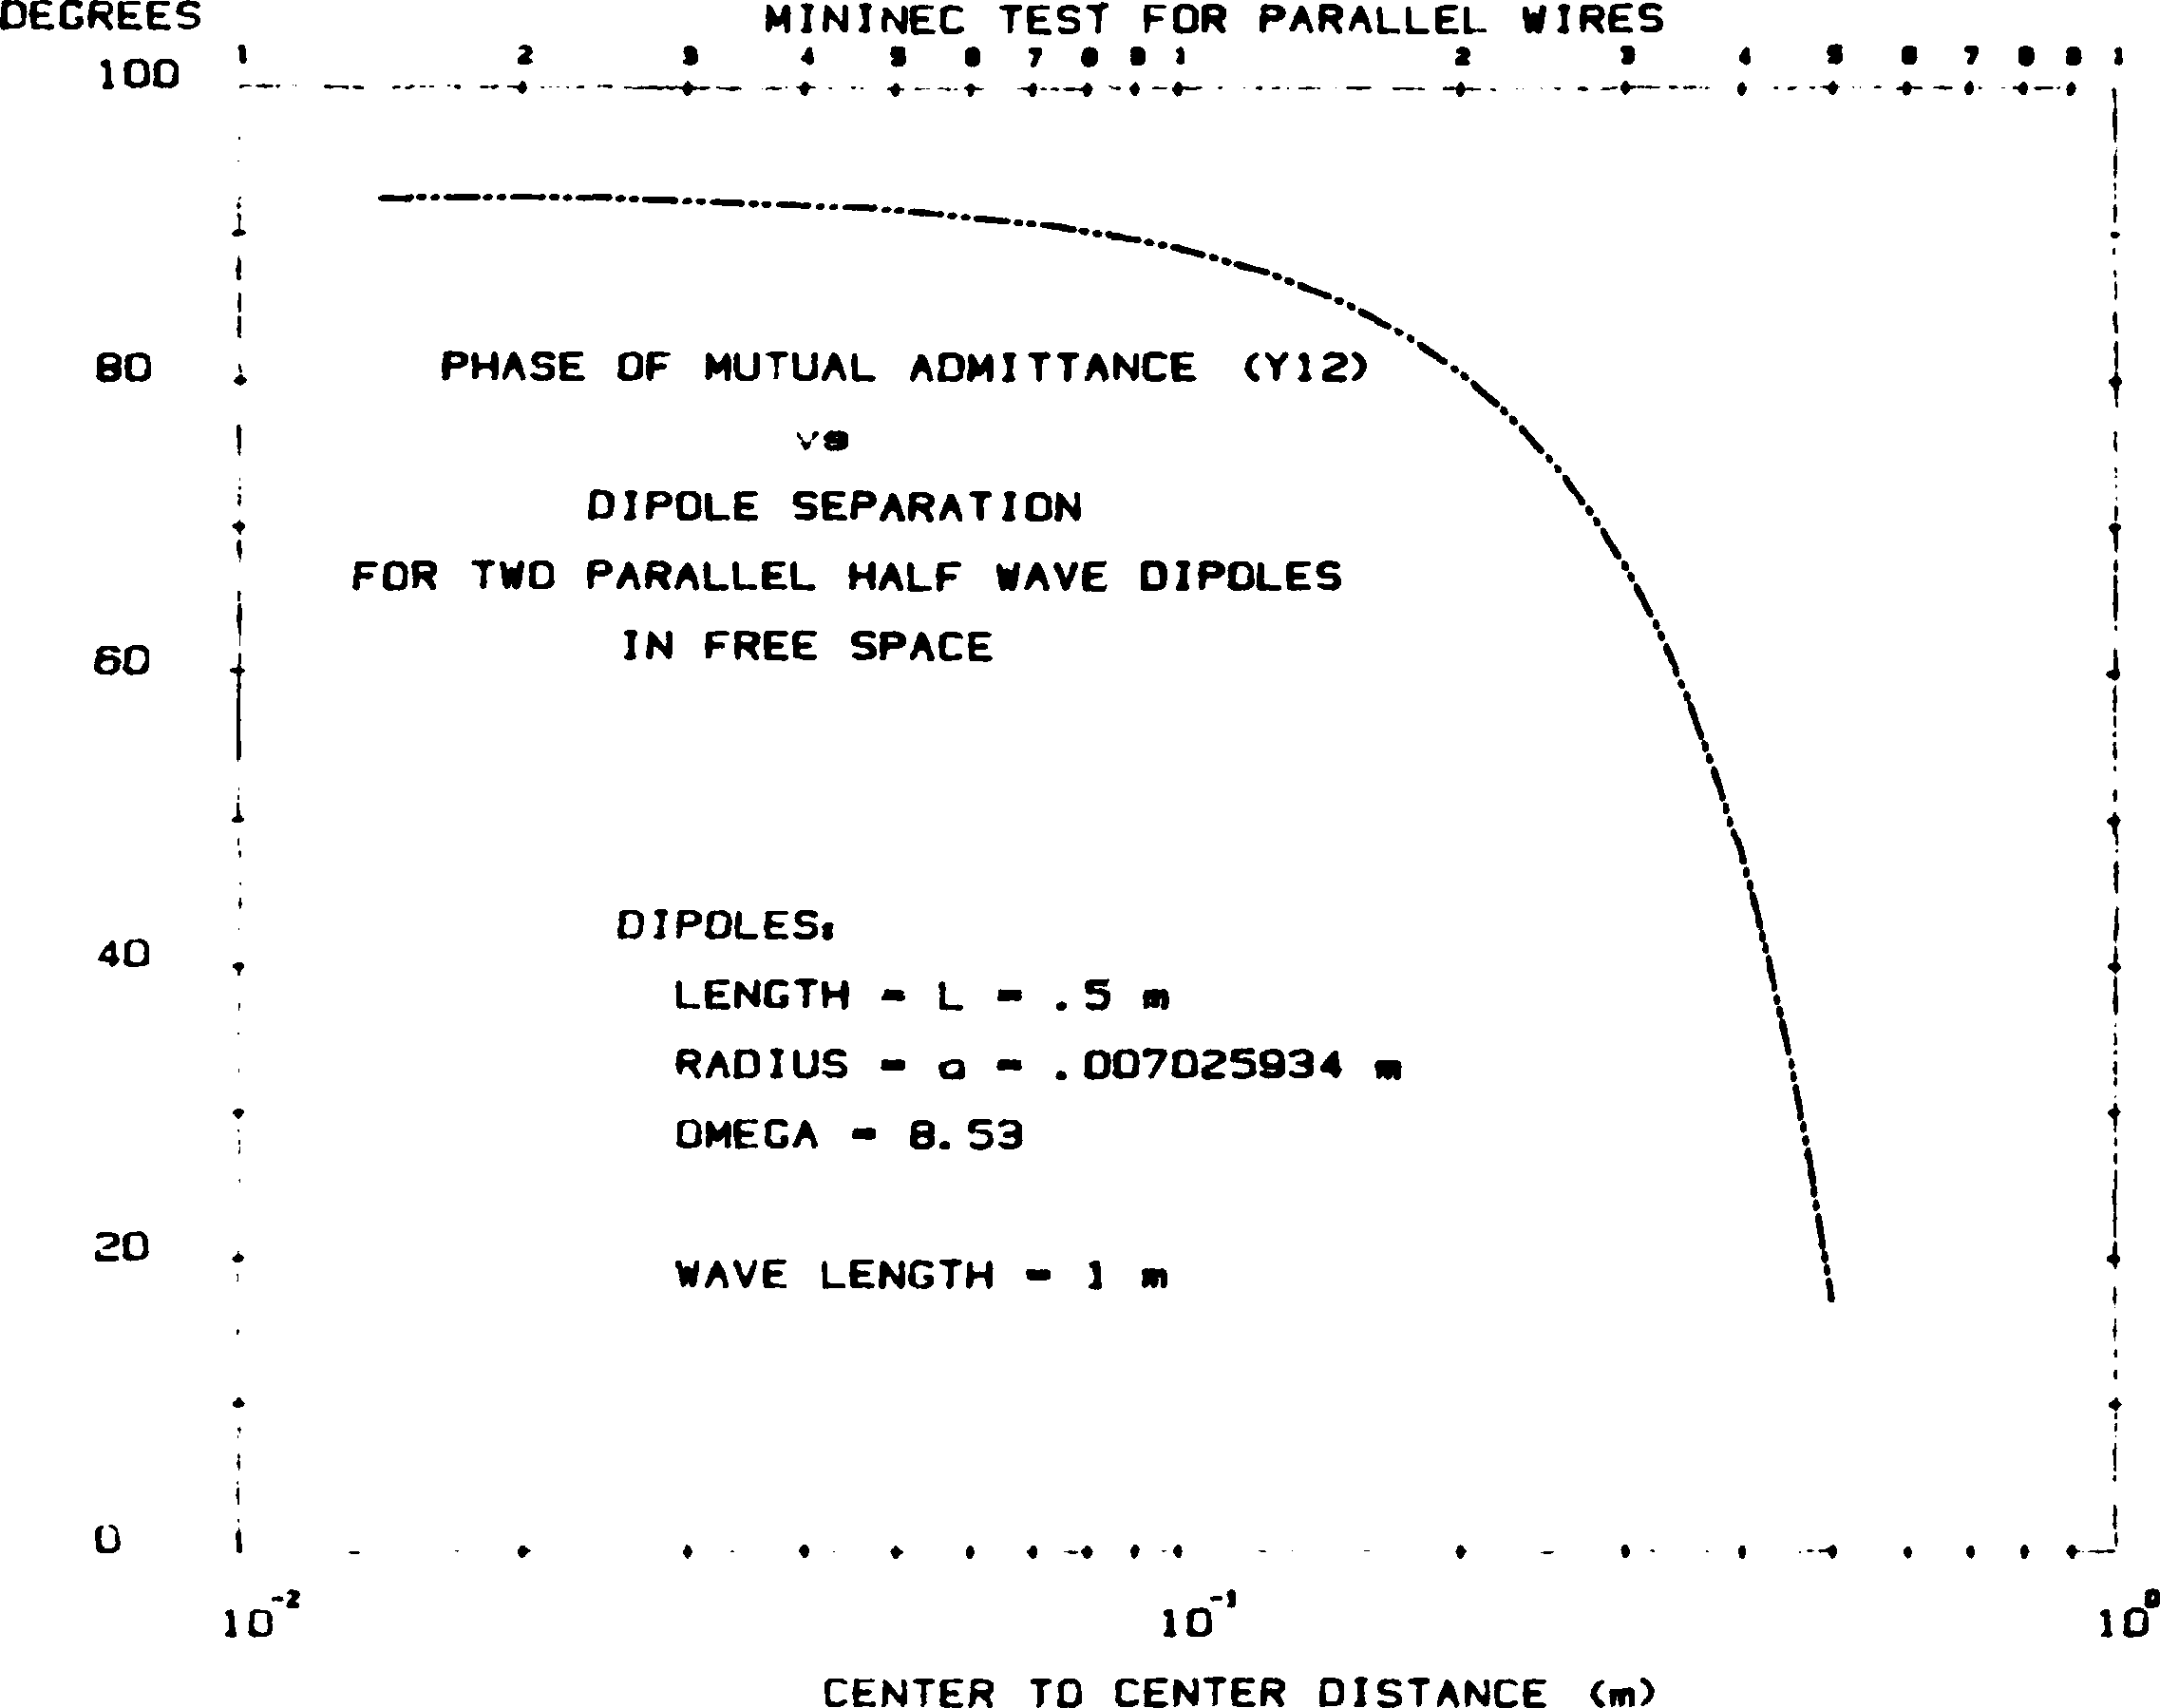
\includegraphics{fig23.eps}}
\caption{Phase of the mutual admittance between closely spaced
parallel dipoles}
\label{fig23}
\end{sidewaysfigure}
\afterpage\clearpage

Figures~\ref{fig16},~\ref{fig17},~\ref{fig18}, and~\ref{fig19} show the
current distribution predicted by PEC, NEC and MININEC for radii steps
of 1:1.25, 1:5, 1:10 and 1:100, respectively. The NEC data are from
their report. The MININEC results follow the PEC data surprisingly well
for all step ratios. (We believe the difference between NEC and PEC may
be an error in the data in the Glisson report. We have not observed this
difference in NEC data.) Further investigation of MININEC for different
stepped radius problems should be conducted. Suggestions include moving
the feed closer to the step and switching the radii $a_1$ and $a_2$.

Multiple wire antenna structures may often require very close spacing.
When the spacing is very small, the currents may not be adequately
represented by a thin filament on the wire axis as it is represented in
MININEC. Figures~\ref{fig20},~\ref{fig21},~\ref{fig22}, and~\ref{fig23}
show MININEC data for a parallel wire test used to investigate the close
spacing limit. The test consists of evaluating the self and mutual
admittance between two parallel half wave dipoles. One antenna is driven
(i.e., the source is in the center pulse) while the second is not. The
self admittance is the feed point current on the first wire if the
applied voltage is 1 + j0 volts and the mutual admittance is the current
for the center pulse of the second wire.

Figure~\ref{fig20} shows the self admittance compared to the theory by
R.W.P. King \cite{r9} for dipole center to center spacings
between .1 and .5 wave length. Figure~\ref{fig21} shows a similar
comparison for the mutual admittance over the same range. The
differences between MININEC and R.W.P. King are mostly less than .2
millimho and are no greater than .4 millimho in the worst case over the
range shown for both self and mutual admittance.

Given the good agreement with theory down to a spacing of .1 wave
length, how does MININEC fare for closer spacing? Figures~\ref{fig22}
and~\ref{fig23} show the magnitude and phase of the mutual admittance
for spacings down to the point of contact of the two parallel dipoles.
Keep in mind the good agreement between MININEC and theory for spacings
of .1 wave length and greater. (Reference~\cite{r9} does not provide
data for spacings less than .1, no comparison is shown.) It can be seen
that the magnitude and phase continue smoothly as the spacing is
reduced. Although these data are not conclusive, it can be implied that
MININEC can model antenna configurations with wire spacings less than .1
wave length. Whenever a model has close spacing, however, it is
advisable to examine the results very closely to ensure proper behavior.

\begin{sidewaysfigure}[htb]
\centerline{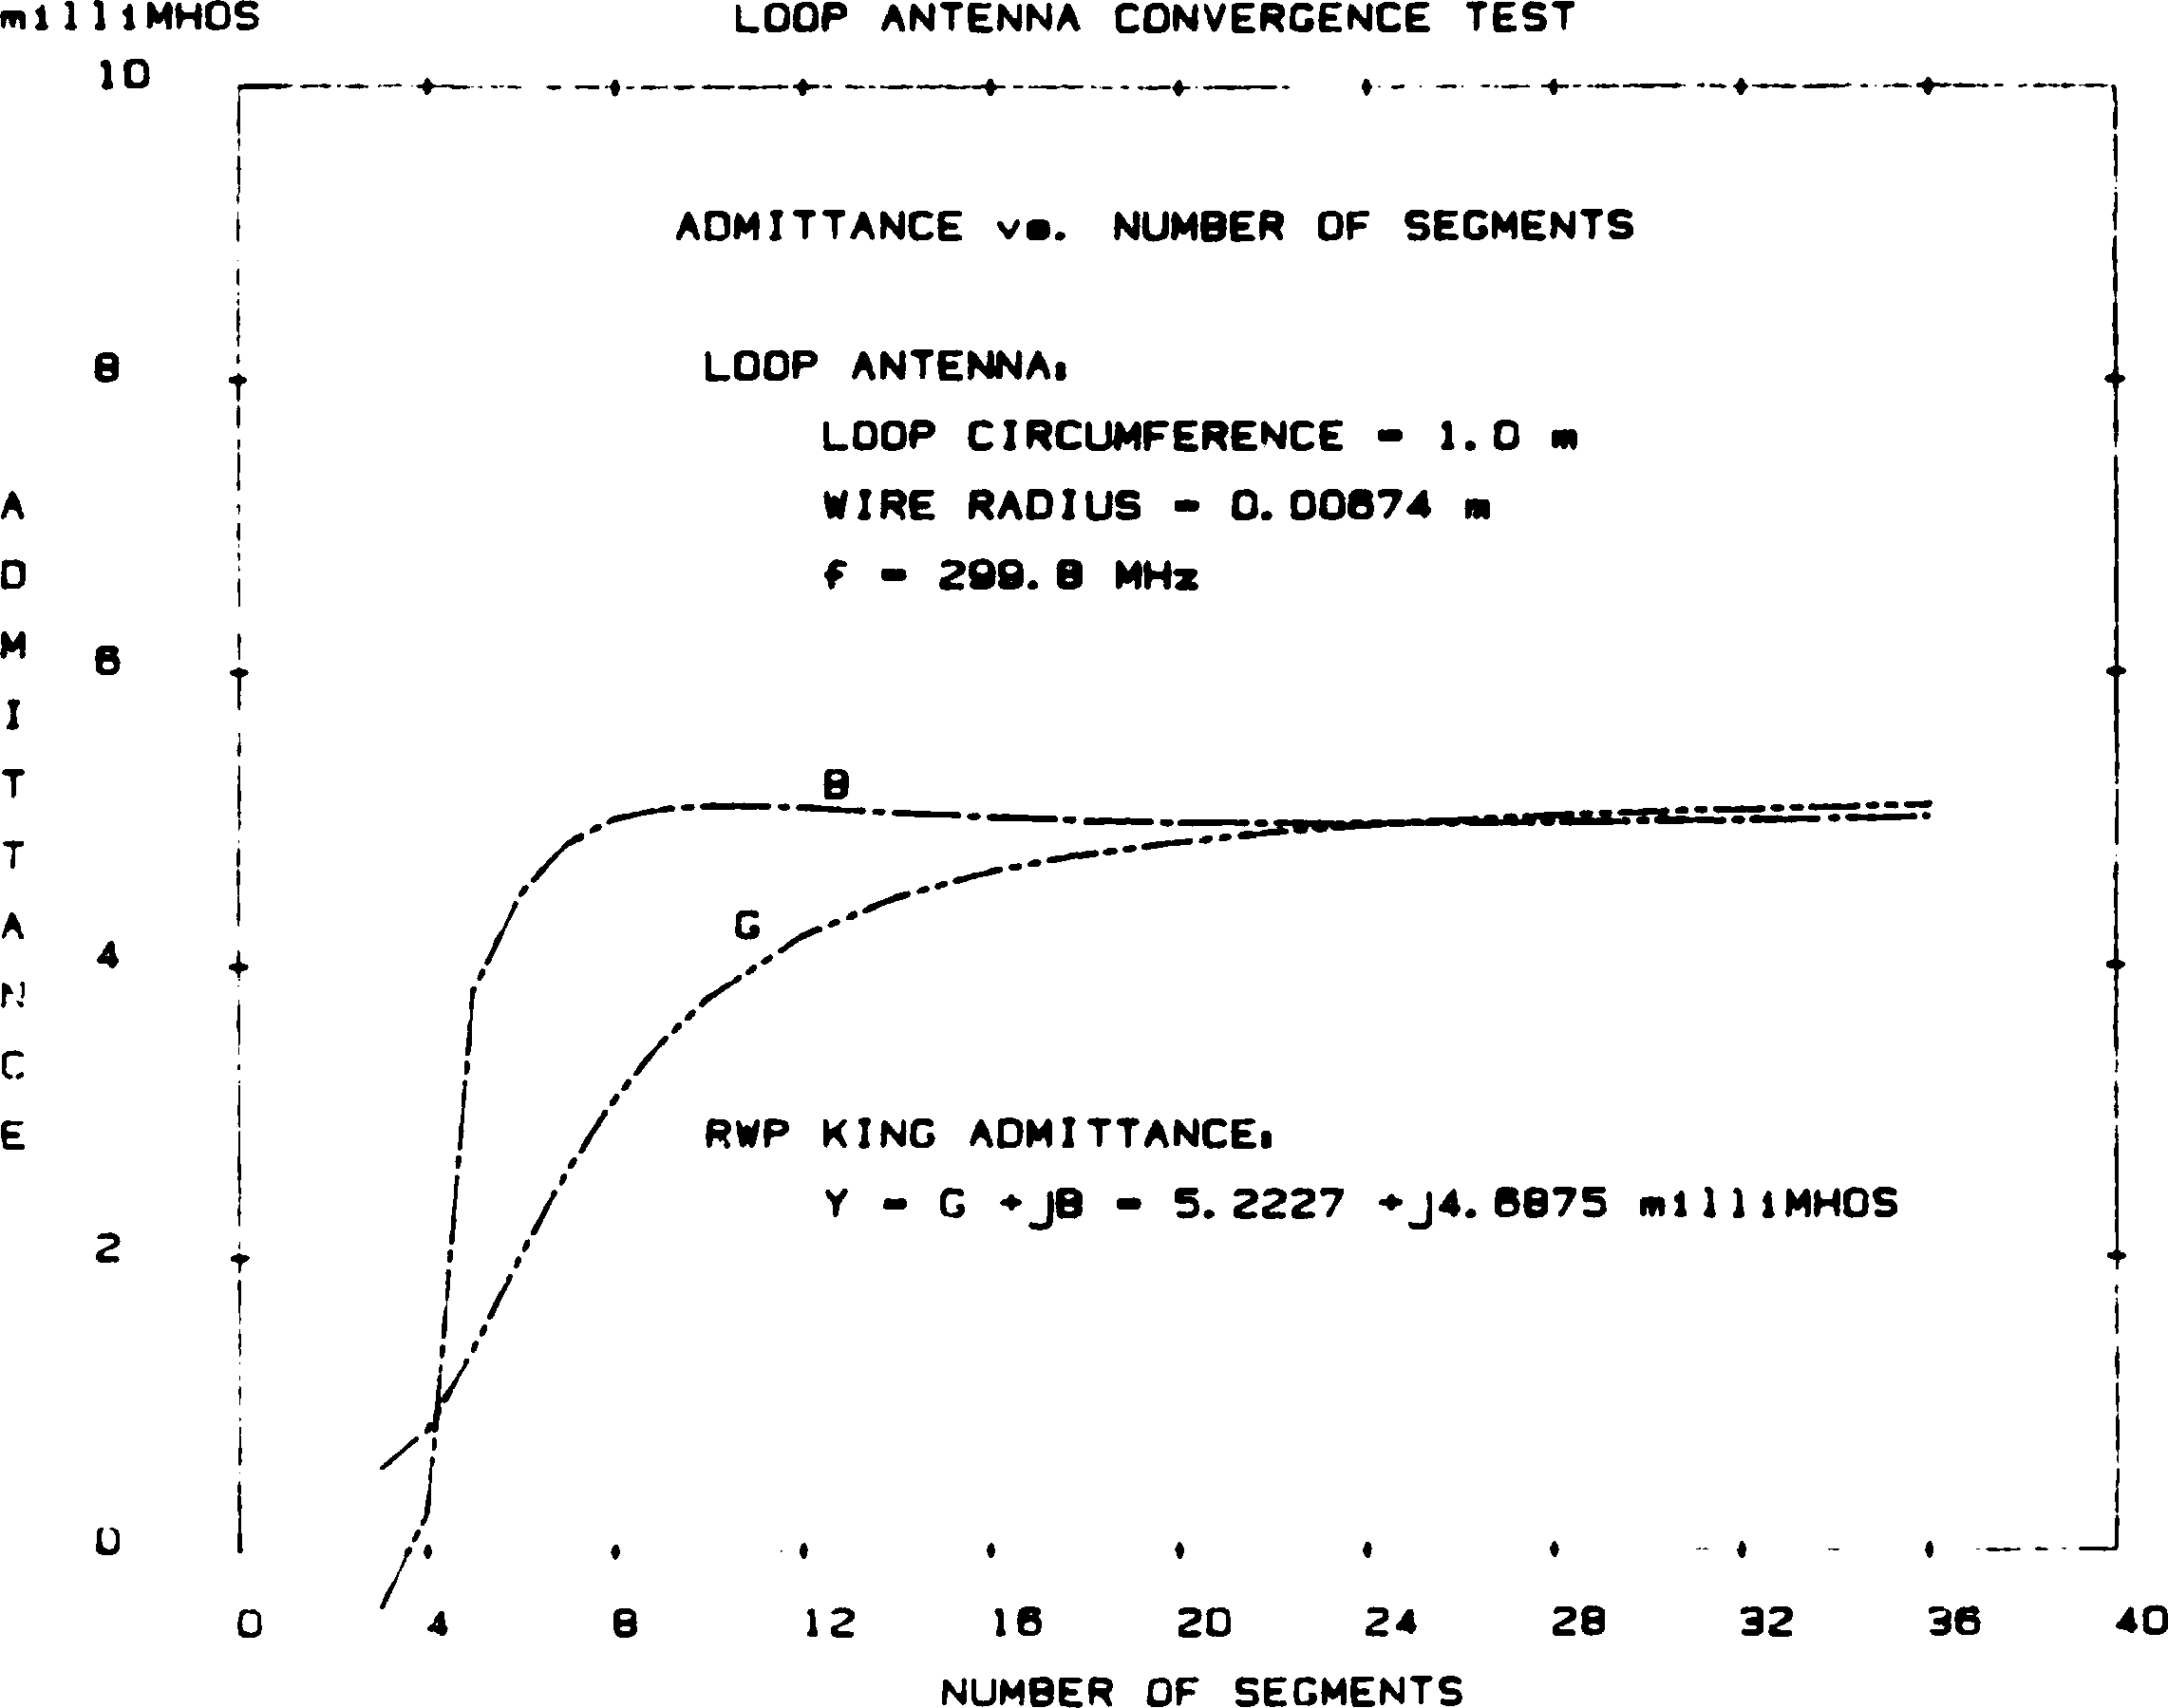
\includegraphics{fig24.eps}}
\caption{Admittance of a polygon model antenna. The polygon is
circumscribed by a circle of one wavelength circumference.}
\label{fig24}
\end{sidewaysfigure}

\begin{sidewaysfigure}[htb]
\centerline{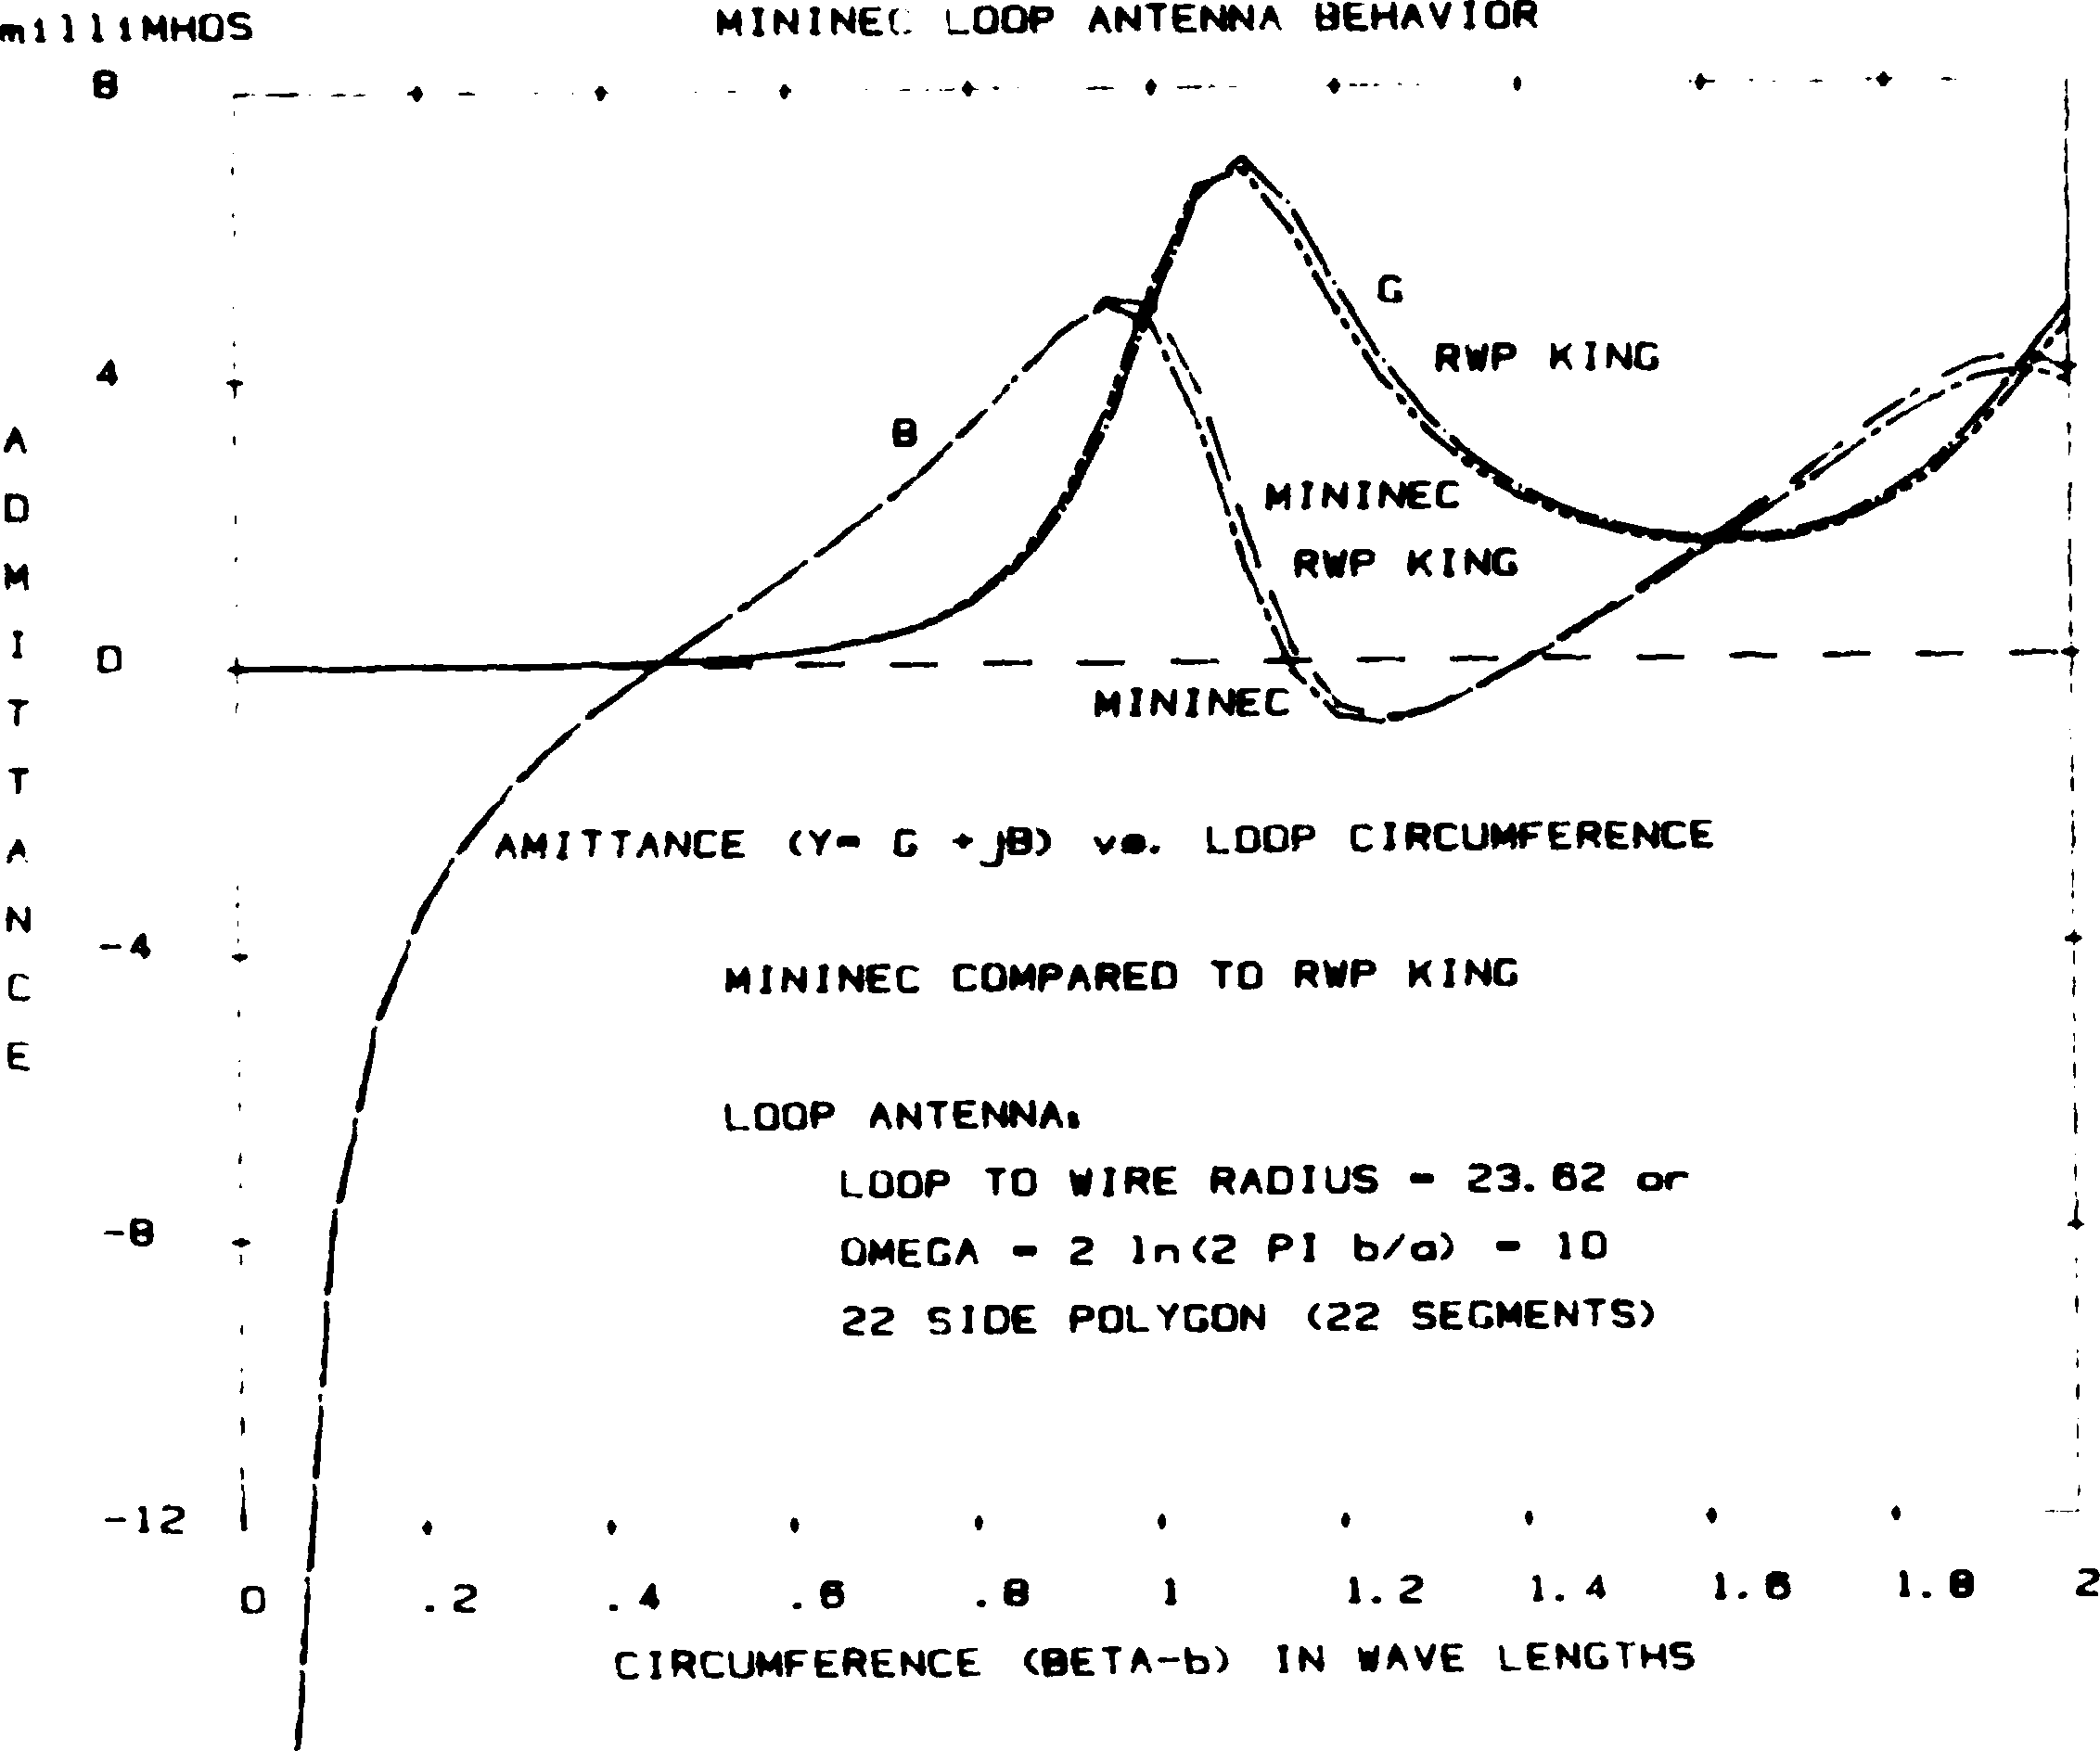
\includegraphics{fig25.eps}}
\caption{A comparison of MININEC data to R. W. P. King over a range of
loop sizes}
\label{fig25}
\end{sidewaysfigure}

\begin{sidewaysfigure}[htb]
\centerline{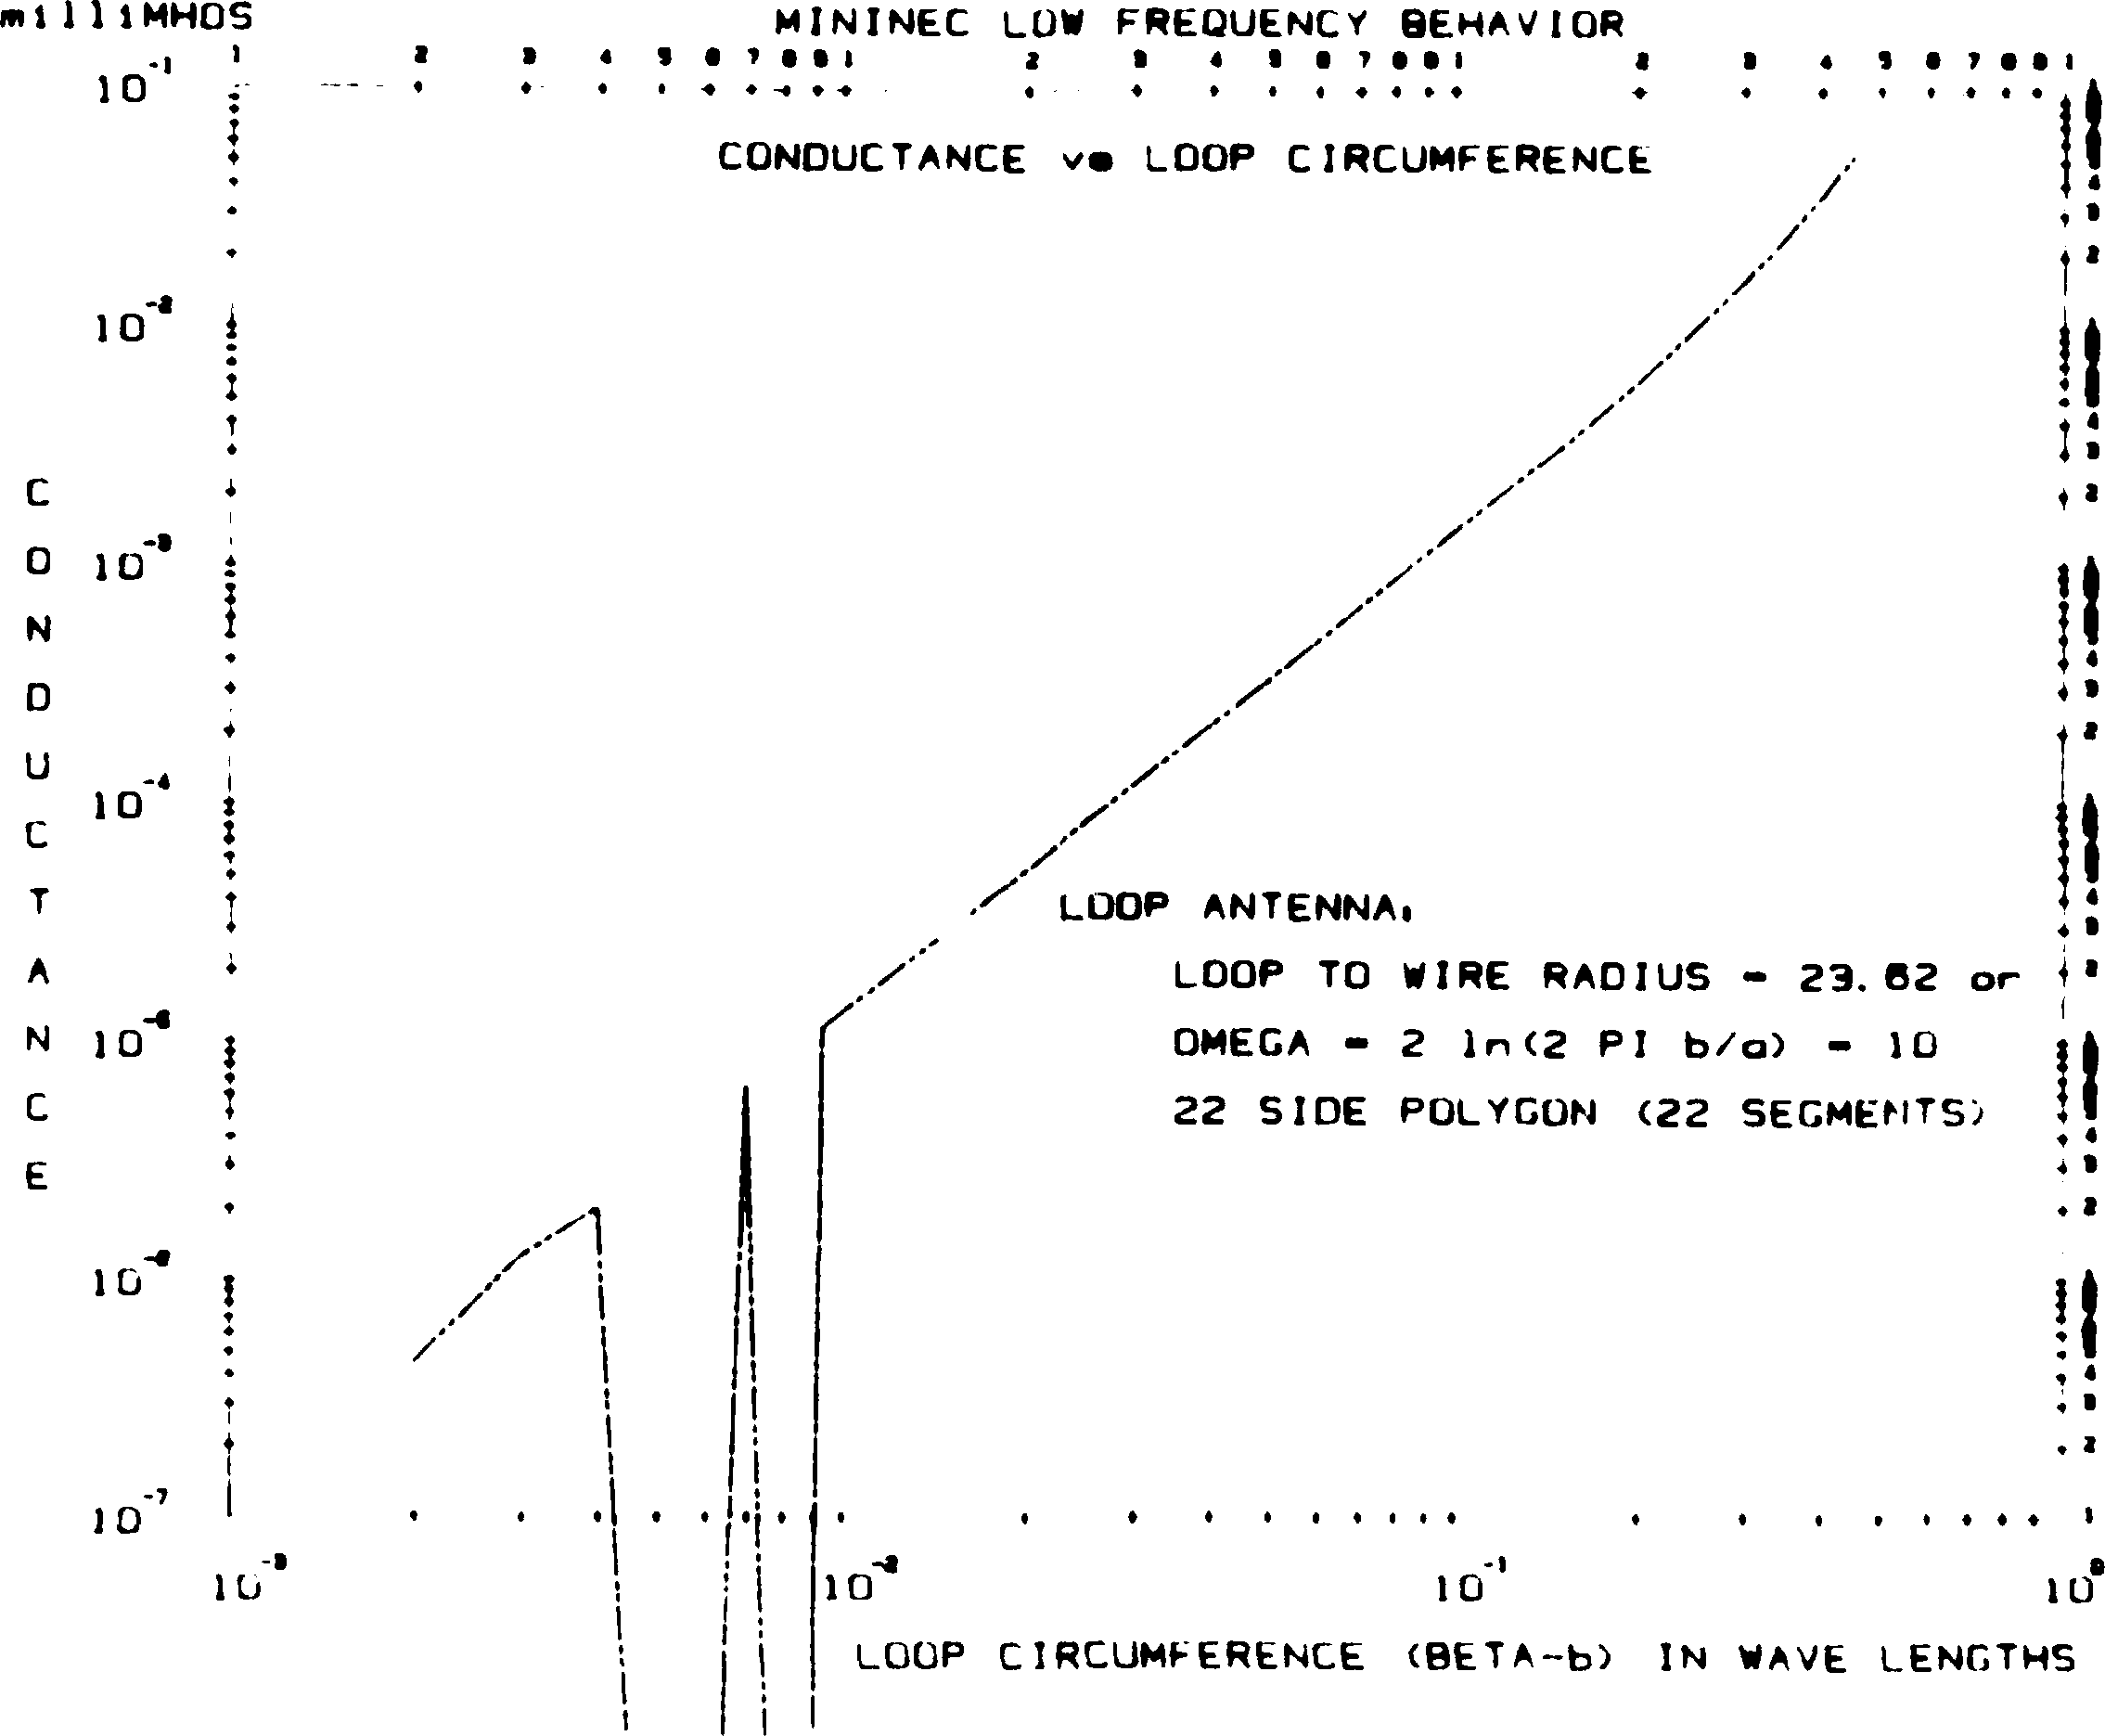
\includegraphics{fig26.eps}}
\caption{Admittance of small loops predicted by MININEC (Part~1)}
\label{fig26}
\end{sidewaysfigure}

\begin{sidewaysfigure}[htb]
\centerline{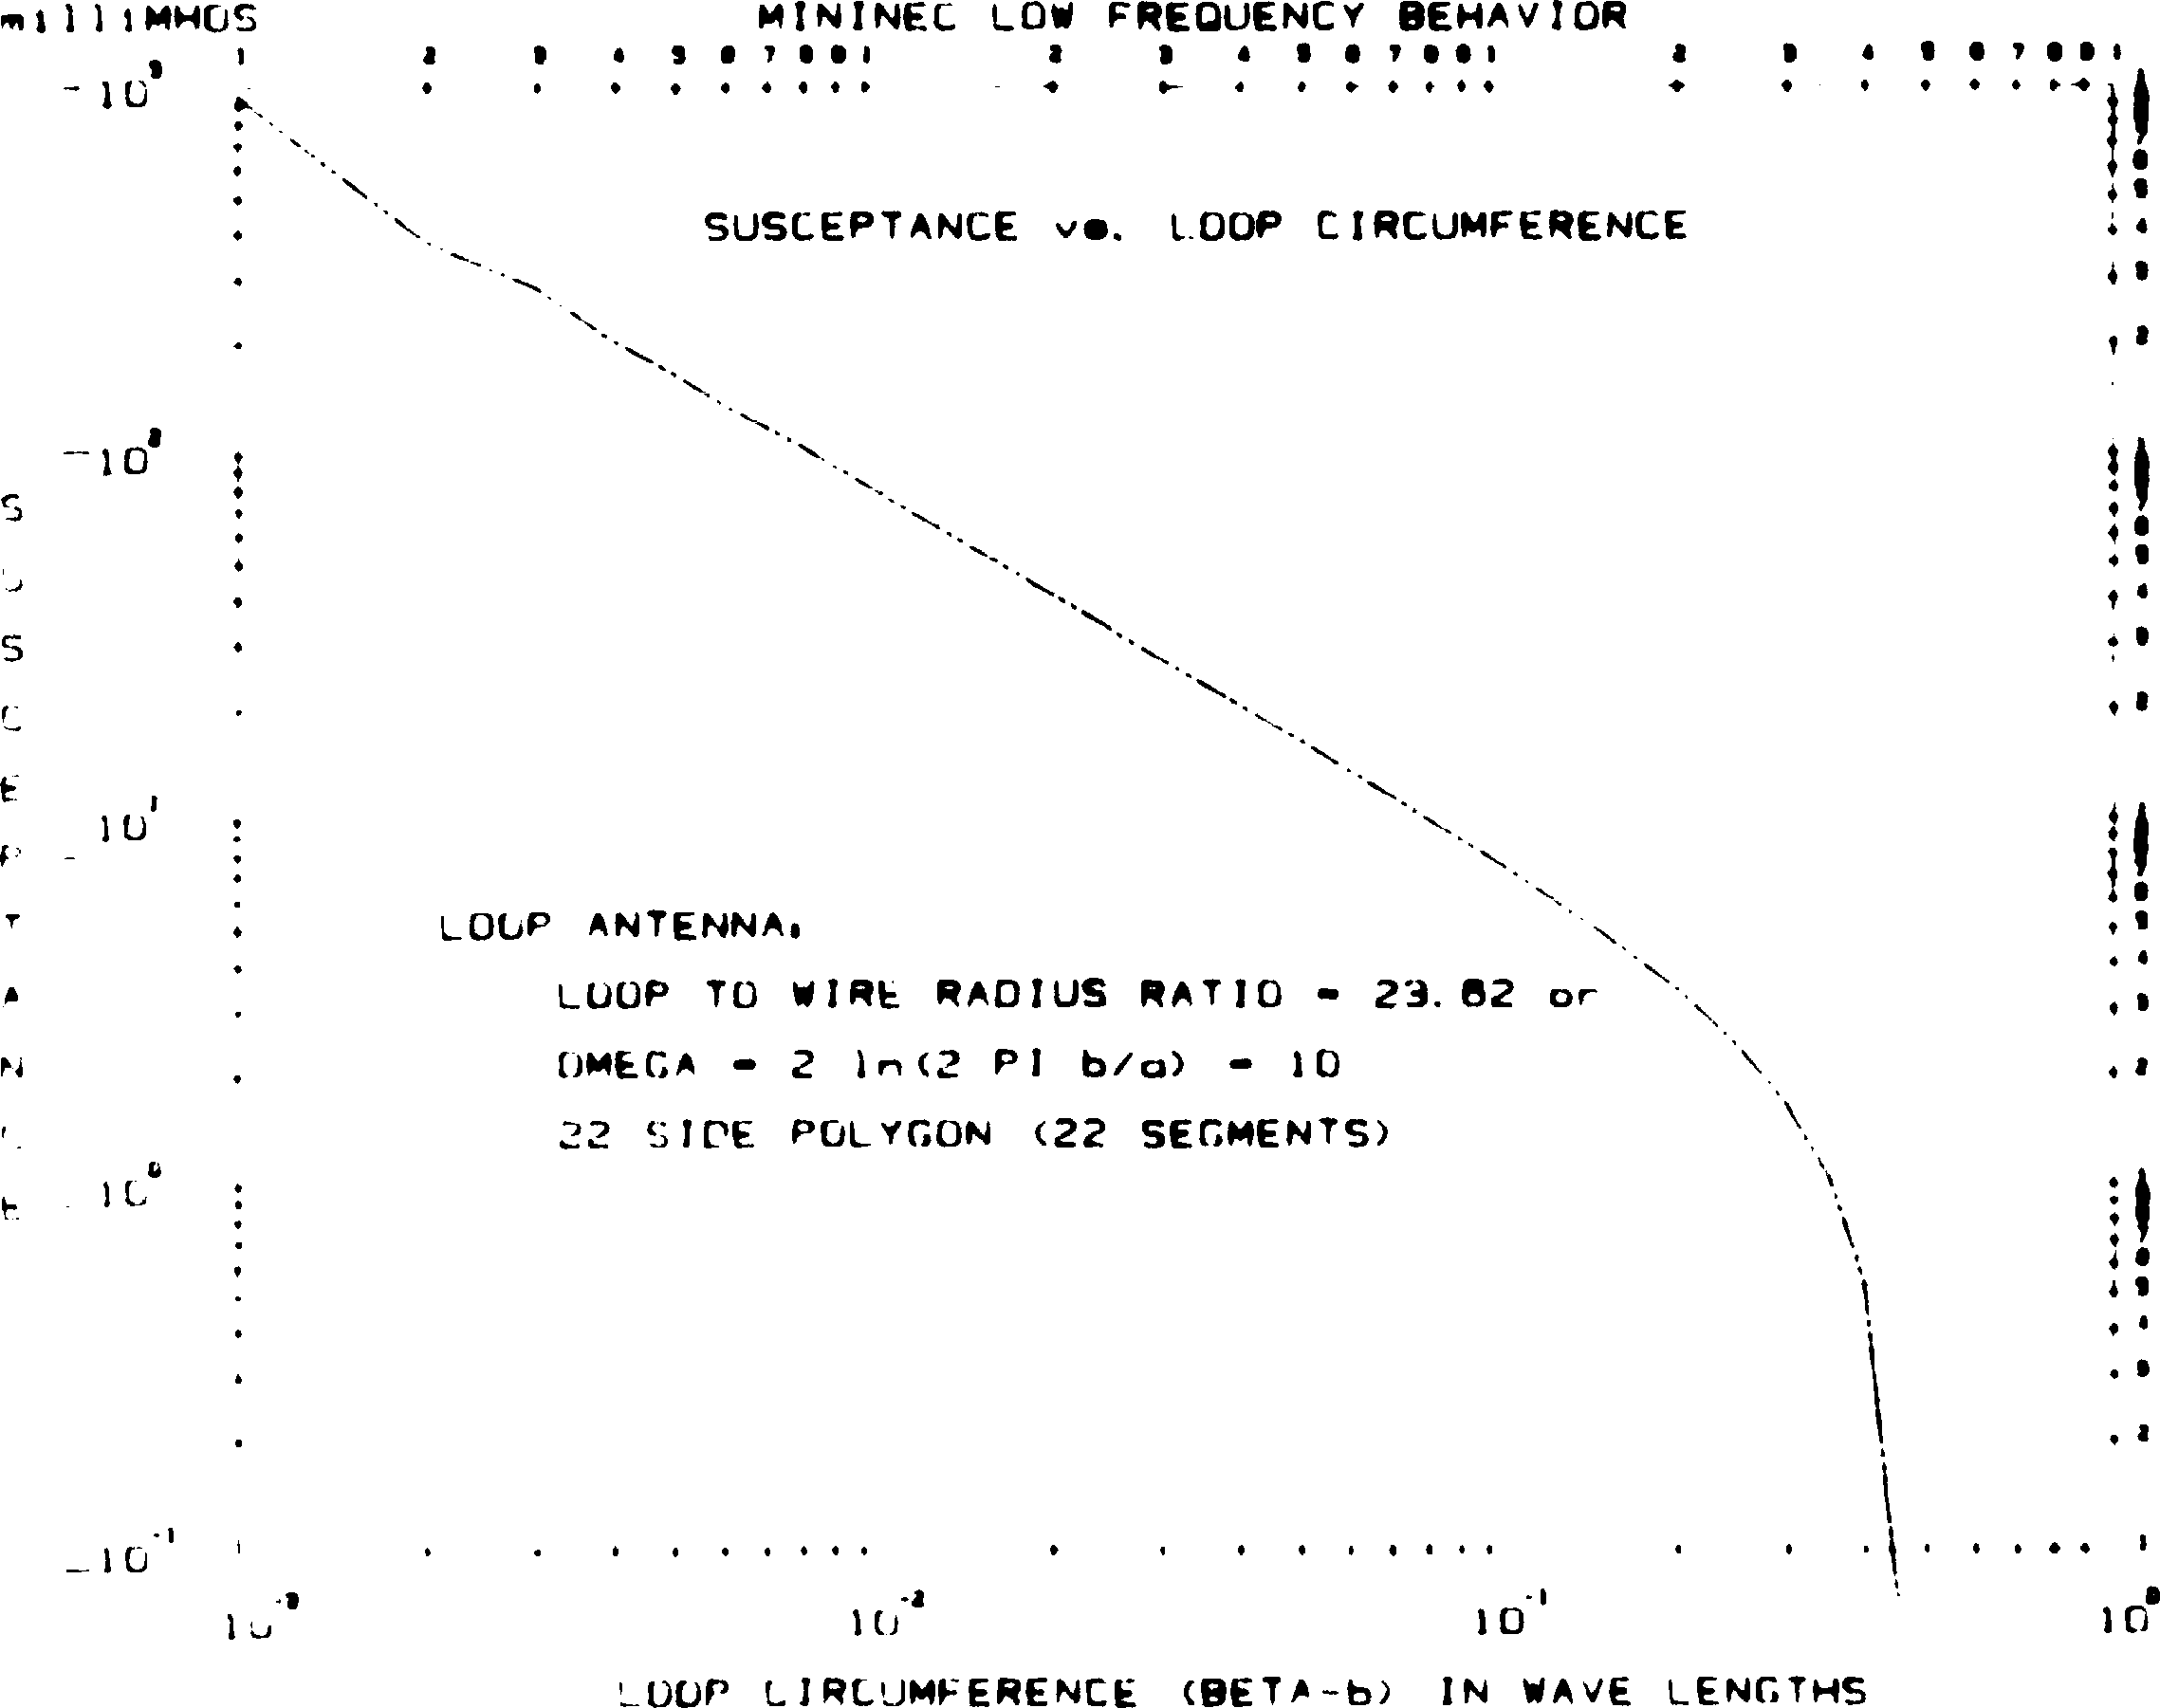
\includegraphics{fig27.eps}}
\caption{Admittance of small loops predicted by MININEC (Part~2)}
\label{fig27}
\end{sidewaysfigure}
\afterpage\clearpage

\subsection{Loop Antennas}
A circular wire loop antenna may be modeled by connecting a number of
wires to form a polygon approximation to the circular loop. A simple
model has one segment per wire, with each wire forming one side of the
polygon model, so that the number of sides and the number of segments
are equal. For a given circumference, the number of wires, and hence the
number of segments, can be increased until the solution stabilizes,
indicating the number of sides required to model the circular loop.
Figure~\ref{fig24} shows the results of this procedure for a loop, one
wave length in circumference. The polygon model is circumscribed by a
circle whose circumference is one wave length. The wire radius
($a=.00674$ meter) is chosen to correspond to the published data given
by R.W.P. King \cite{r9}. At best, the real part of the
MININEC admittance comes to within 3\% of King's data and the imaginary
part approaches to within 6\%. For 22 segments (and 22 sides) the
percent difference in real and imaginary is about equal, and less than
6\% for each.

Figure~\ref{fig25} compares MININEC and R.W.P. King admittance data for
a range of loop diameters from .1 to 2.0 wave lengths. The MININEC model
is the 22 segment or 22 sided polygon loop. The agreement is excellent.
The difference between King and MININEC is no greater than .4 millimho
over the entire range. From .1 to .8 wave length, the MININEC data and
King data are virtually identical.

Figures~\ref{fig26} and~\ref{fig27} show MININEC data for small loops
with a circumference from $10^{-3}$ to just above .4 wave length. Keep
in mind the excellent agreement with King's data for loops of .1 and
greater (Figure~\ref{fig25}). The real and imaginary parts of the
adminttance in Figures~\ref{fig26} and~\ref{fig27}, respectively, are
well behaved for loops greater than $10^{-2}$ wave lengths. Below
$10^{-2}$, the real part of the admittance becomes unstable due to
numerical problems encountered at the limits of single precision. Note
that at 22 segments, the segment size at a circumference of $10^{-3}$,
is very nearly the same short segment length limit displayed by the
dipole test in Figure~\ref{fig14}. The data in
Figures~\ref{fig25},~\ref{fig26}, and~\ref{fig27} suggest a small loop
limit for MININEC (on a 16-bit, single precision microcomputer) of
$10^{-2}$ wave lengths in circumference. This corresponds to a loop 18
inches in diameter at 2~MHz (about the size of a basketball goal).

% unreadable: figure caption
% unreadable: figure table entries on left side
\begin{figure}[htb]
\begin{center}
\vspace*{-5mm}
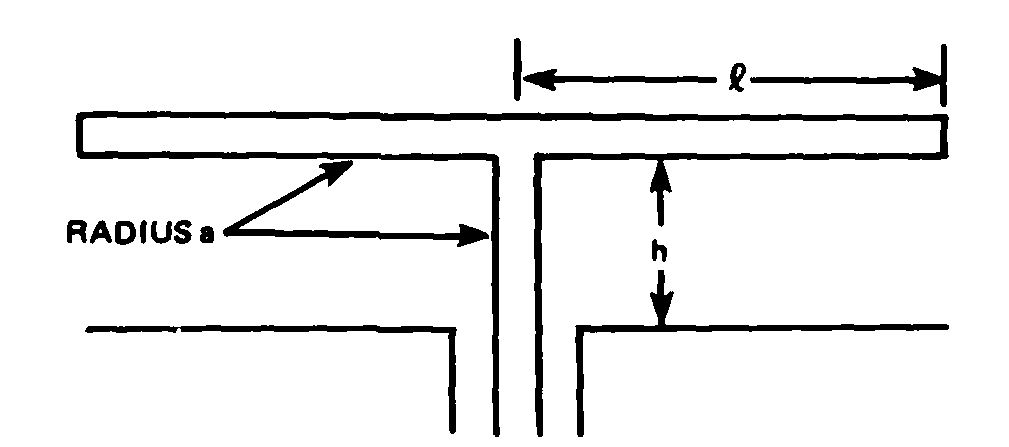
\includegraphics{fig28.eps}\\
\ \\
\begin{tabular}{r|r|r|r}
$K_0h$ & $h/\lambda$ & $\ell/\lambda$ \\[3pt]
\cline{1-3}
       &             &                    \\[-8pt]
0.2    & 0.03183099  & 0.2181690          \\
0.5    & 0.07957747  & 0.1704225          \\
\multicolumn{4}{c}{}               \\
                                   &
                                   &
\multicolumn{1}{c|}{Horizontal}    &
                                   \\
\multicolumn{1}{c|}{$K_0h$}        &
\multicolumn{1}{c|}{Vertical Wire} &
\multicolumn{1}{c|}{Wire}          &
\multicolumn{1}{c}{Total}          \\
                                   &
\multicolumn{1}{c|}{Segments}      &
\multicolumn{1}{c|}{Segments}      &
\multicolumn{1}{c}{Segments}       \\
\hline
0.2 &  1  &  7 & 15 \\
    &  2  & 14 & 30 \\
    &  3  & 21 & 45 \\
    &  4  & 28 & 60 \\
\hline
0.5 &  1  &  2 &  5 \\
    &  2  &  4 & 10 \\
    &  3  &  6 & 15 \\
    &  4  &  8 & 20 \\
    &  5  & 10 & 25 \\
    &  6  & 12 & 30 \\
    & 14  & 14 & 42 \\
\end{tabular}
\end{center}
\caption{[\ldots] TEE antenna. Dimensions for two designs are given [\ldots]
segmentation scheme for convergence testing}
\label{fig28}
\end{figure}

\begin{sidewaysfigure}[htb]
\centerline{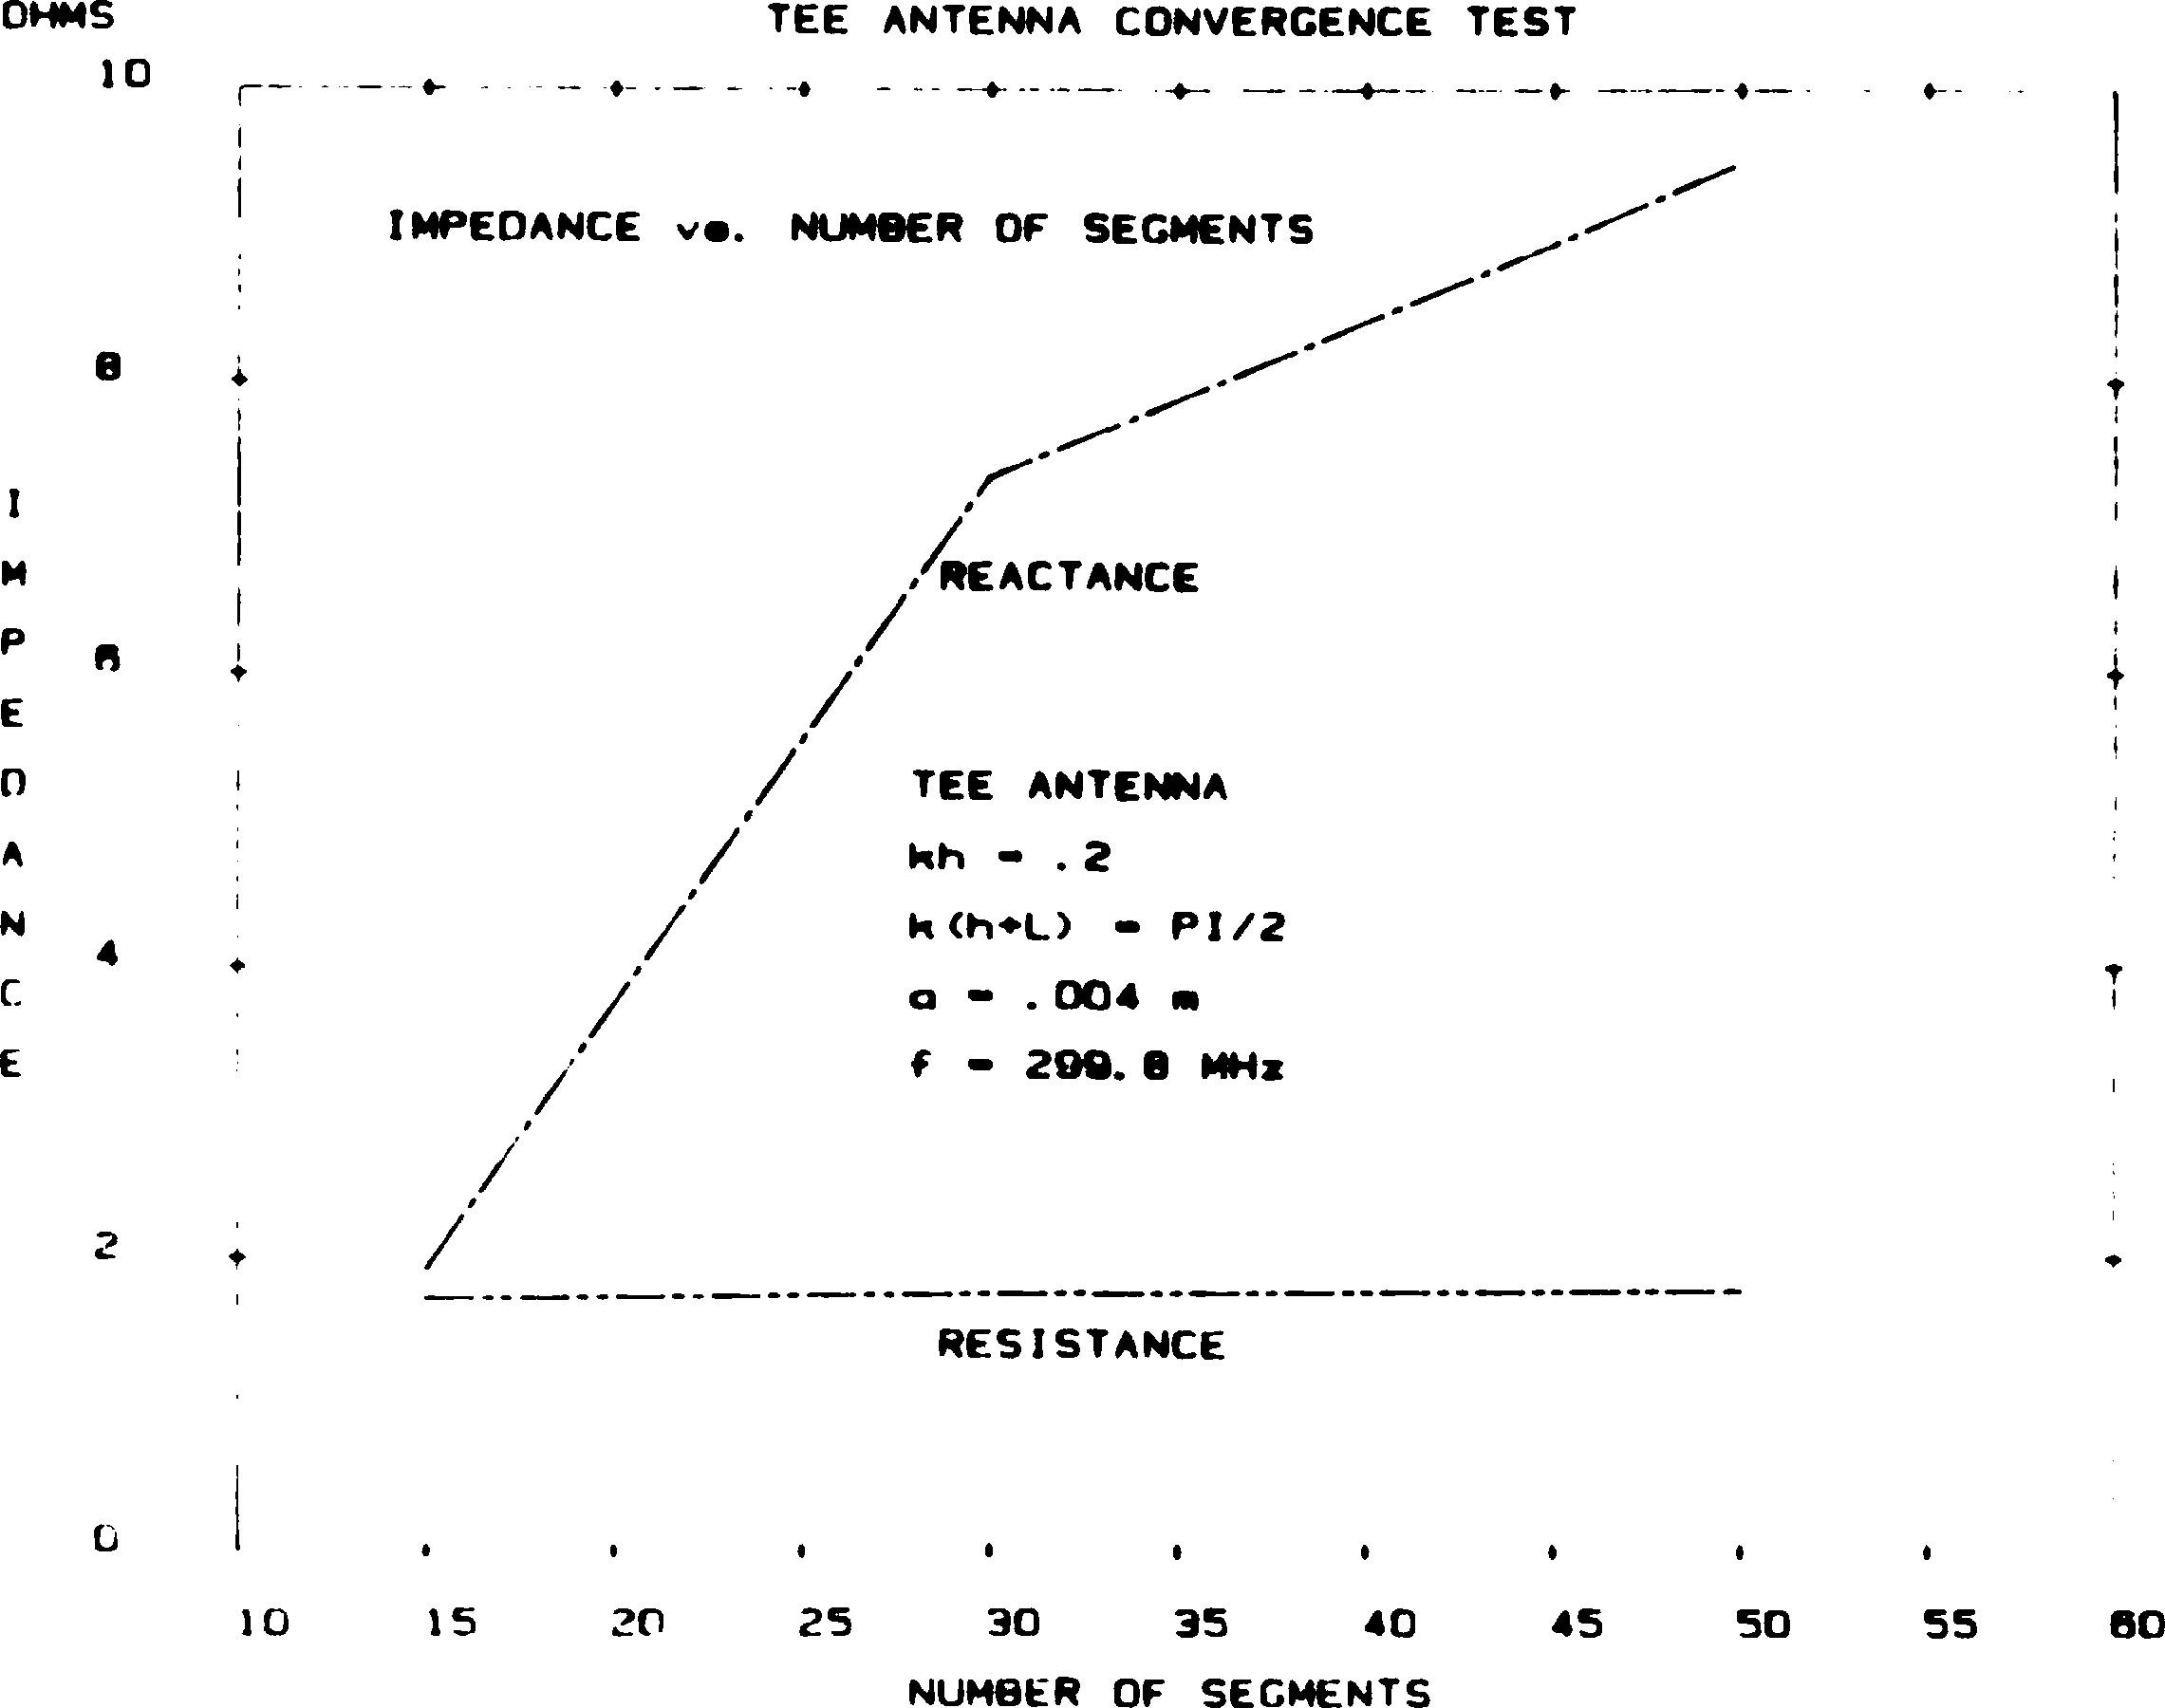
\includegraphics{fig29.eps}}
\caption{Convergence test for a TEE antenna with $K_0 h = .2$}
\label{fig29}
\end{sidewaysfigure}

\begin{sidewaysfigure}[htb]
\centerline{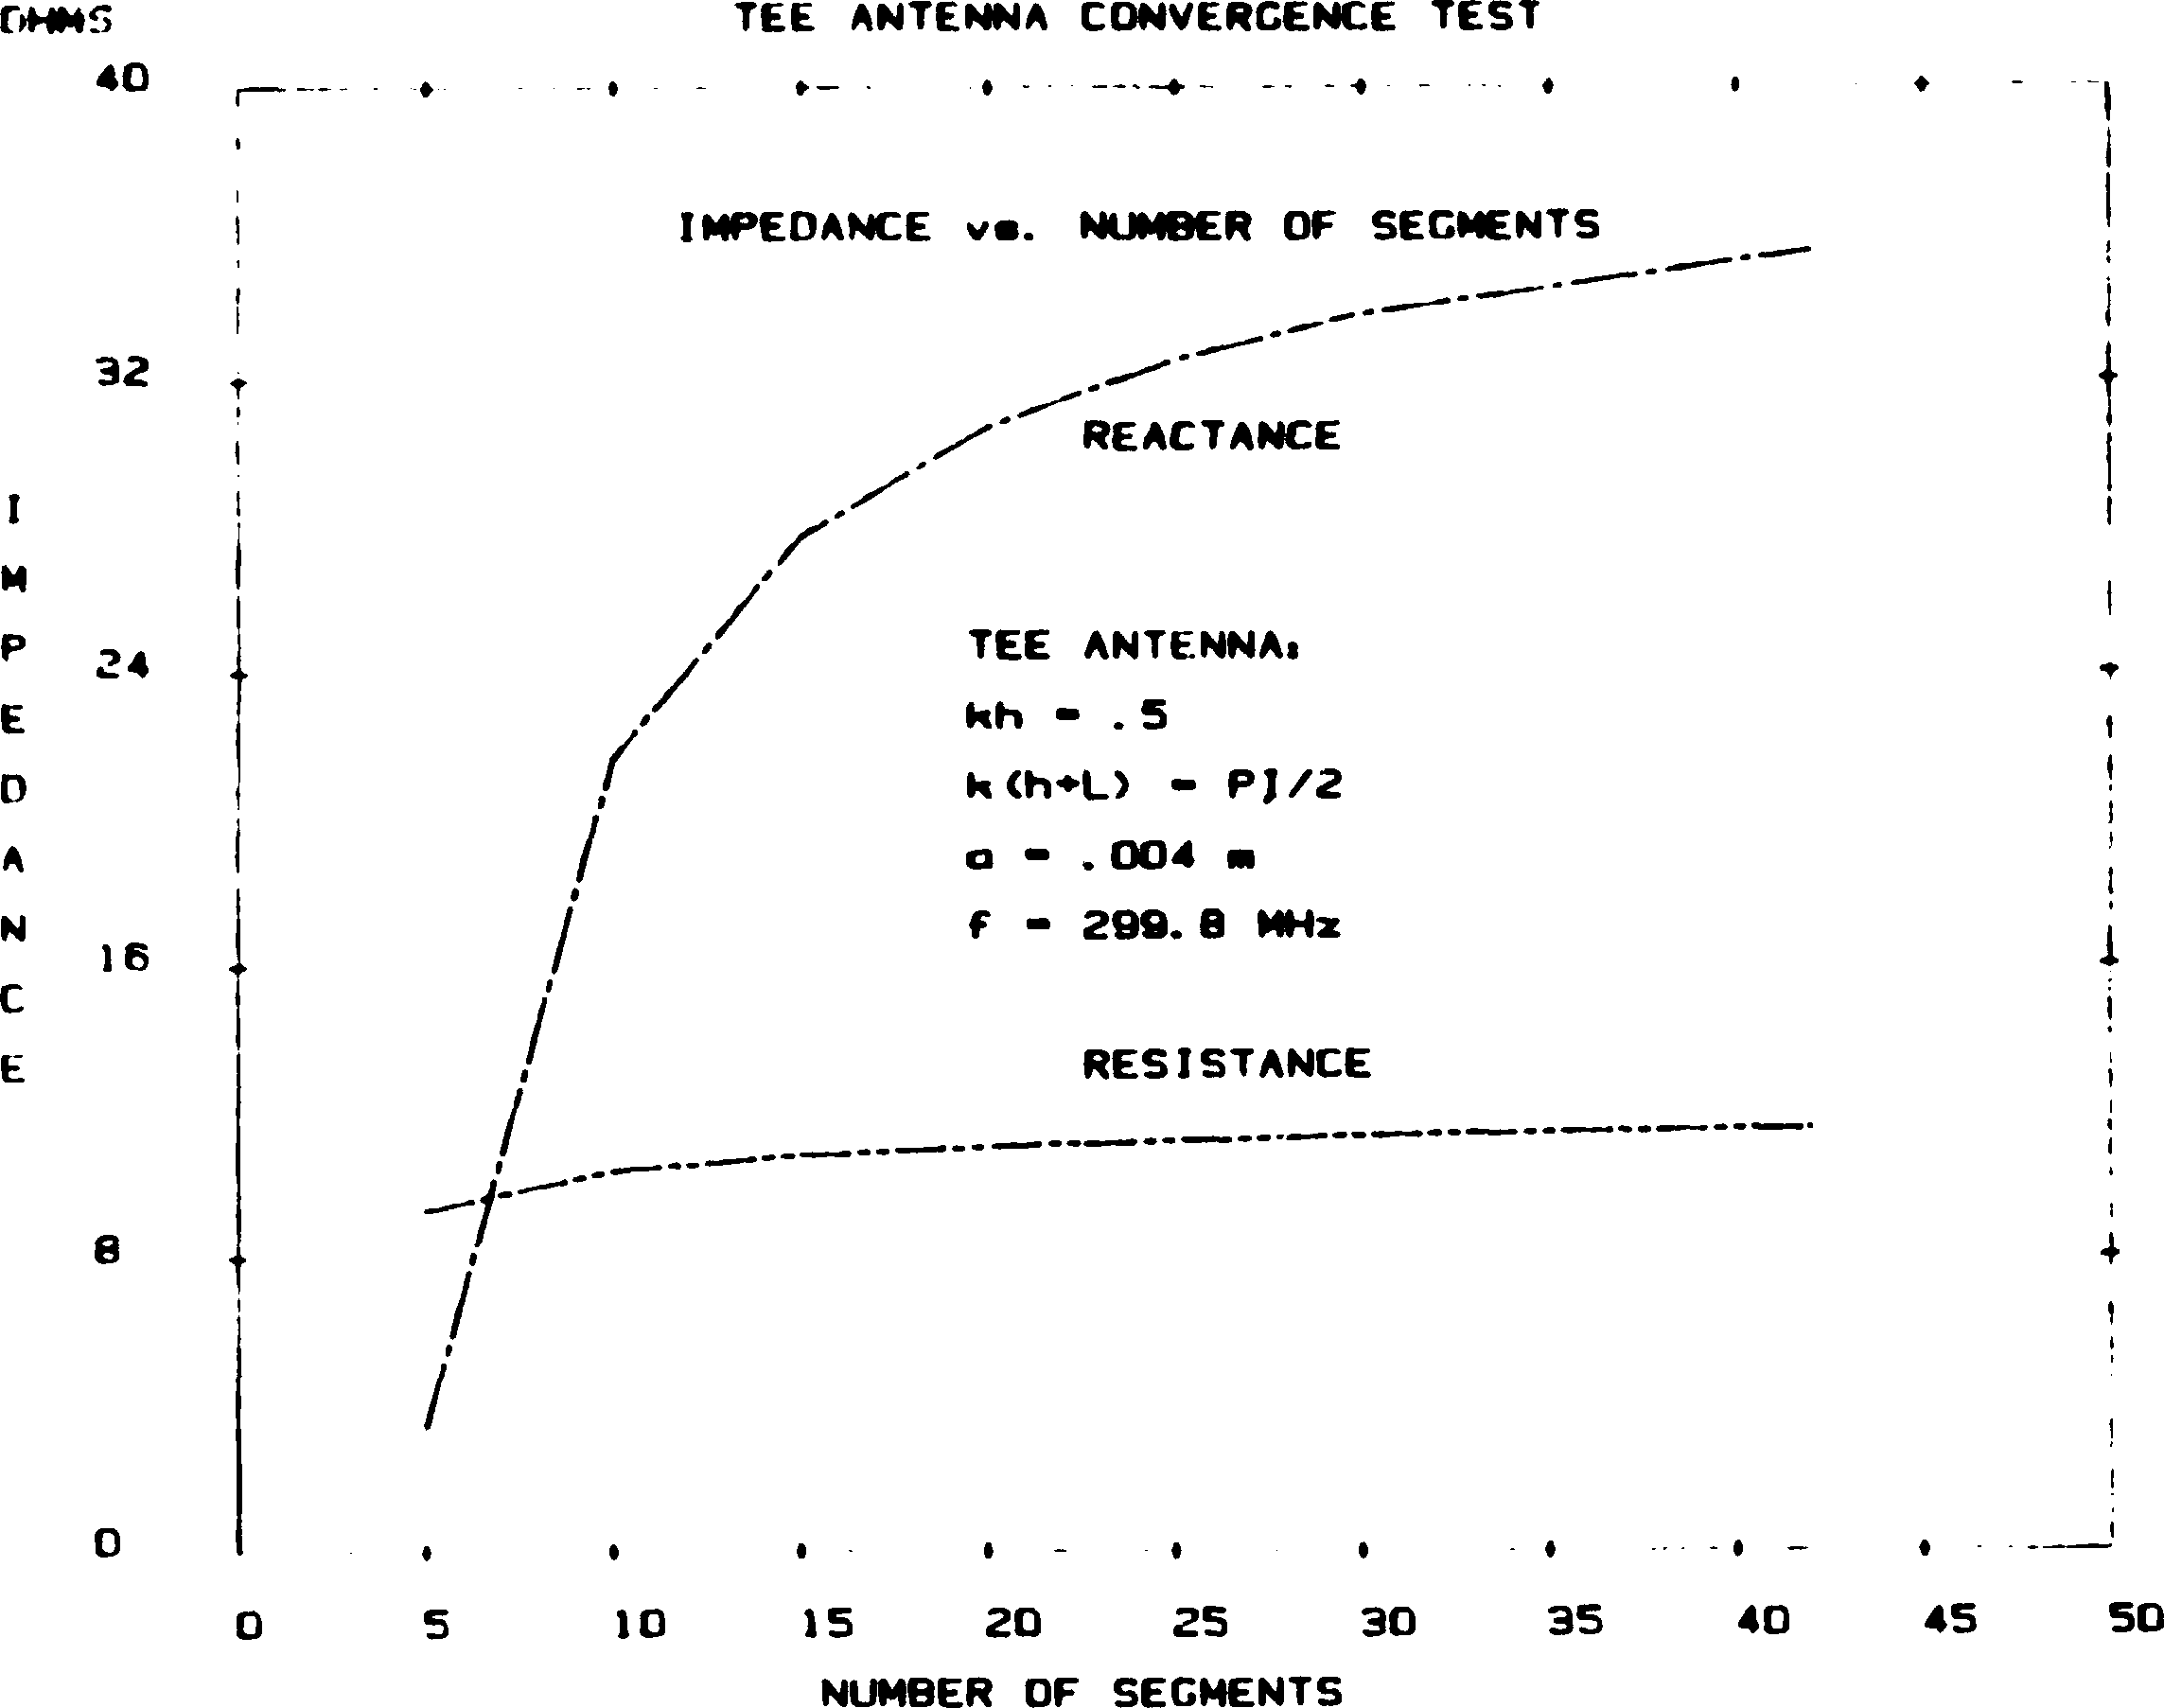
\includegraphics{fig30.eps}}
\caption{Convergence test for a TEE antenna with $K_0 h = .5$}
\label{fig30}
\end{sidewaysfigure}

\subsection{Monopoles and Antennas Above Ground}
\label{sec-monopoles}
Simply stated, an antenna above a perfectly conducting ground plane is
equivalent to the original antenna and its mirror image in free space.
Hence, all the modeling results and guidelines presented so far are
directly applicable to monopoles. Specifically, the convergence
properties illustrated in Figures~\ref{fig6} through~\ref{fig11} can be
used for the initial selection of the segmentation required for a
monopole. However, this should not preclude convergence testing whenever
possible.

Figure~\ref{fig28} illustrates the geometry of a TEE-antenna. The
antenna is driven or fed at its base from a coaxial termination at the
ground plane. The dimensions for two TEE-antenna designs ($K_0 h = .2$
and $K_0 h = .5$) are also given. A convergence test was performed for
each antenna using the segmentation scheme in the table. The results of
these tests are given in Figures~\ref{fig29} and~\ref{fig30} for
$K_0 h = .2$ and $K_0 h = .5$, respectively. A comparison of the
``best'' results to the measurements of Prasad and King
\cite{r18} for MININEC and several other codes is given in
Figure~\ref{fig31}.

Figure~\ref{fig31} compares five computer programs including MININEC for
the two TEE-antennas. In each case, the programs were tested for
convergence and the best answer with respect to Prasad's measurements is
given. NEC is the code previously described \cite{r4}. TGP
(Triangular-Galerkin Procedure) is the code written by Chao and Straight
\cite{r11} using triangular expansion and testing functions
in a Galerkin procedure (i.e., triangles for both testing and expansion
functions). PSRT (Piece-wise Sinusoidal Reaction Technique) is a
sinusoidal Galerkin code written by Richmond \cite{r19}.
TWTD (Thin Wire Time Domain) is a time domain method of moments code
written by Van Blaricum and Miller \cite{r20}. TWTD uses
subsection collocation (quadratic interpolation with point matching) to
solve for the time-dependent induced currents and time-dependent
radiated fields. Admittance data are obtained from a discrete Fourier
transform of the source current. All codes except MININEC are in FORTRAN
and require mainframe (large) computers. The data show that MININEC can
provide equally accurate answers.

\clearpage

\begin{figure}[htb]
\begin{tabular}{lll}
\multicolumn{2}{l}{\quad Radius of Wire = $0.004/\lambda$}  \\
\multicolumn{2}{l}{\quad $k_0 = (h + l) = \pi/2$}           \\
         & $\frac{2\pi h}{\lambda}=0.2$ & $\frac{2\pi h}{\lambda}=0.5$ \\
\ \\
\hline
\ \\
MEASURED & $2.6+\jj9.0$                 & $11+\jj36$      \\
MININEC  & $1.8+\jj9.0$                 & $11.6+\jj35.5$  \\
NEC      & $1.7+\jj10.3$                & $11+\jj36$      \\
TGP      & $1.78+\jj9.13$               & $11.1+\jj34.3$  \\
PSRT     & $1.7+\jj3.8$                 & $11.4+\jj31.9$  \\
TWTD     &                              & $11+\jj34$      \\
\end{tabular}
\caption{Comparison of TEE-antenna impedance computations with the
measured values of Parsad.}
\label{fig31}
\end{figure}

\subsection{Near Fields}
MININEC can calculate the near fields for antennas in free space and
over perfectly conducting ground. Only antennas over perfectly
conducting ground are considered in this section.

\begin{figure}[htb]
\centerline{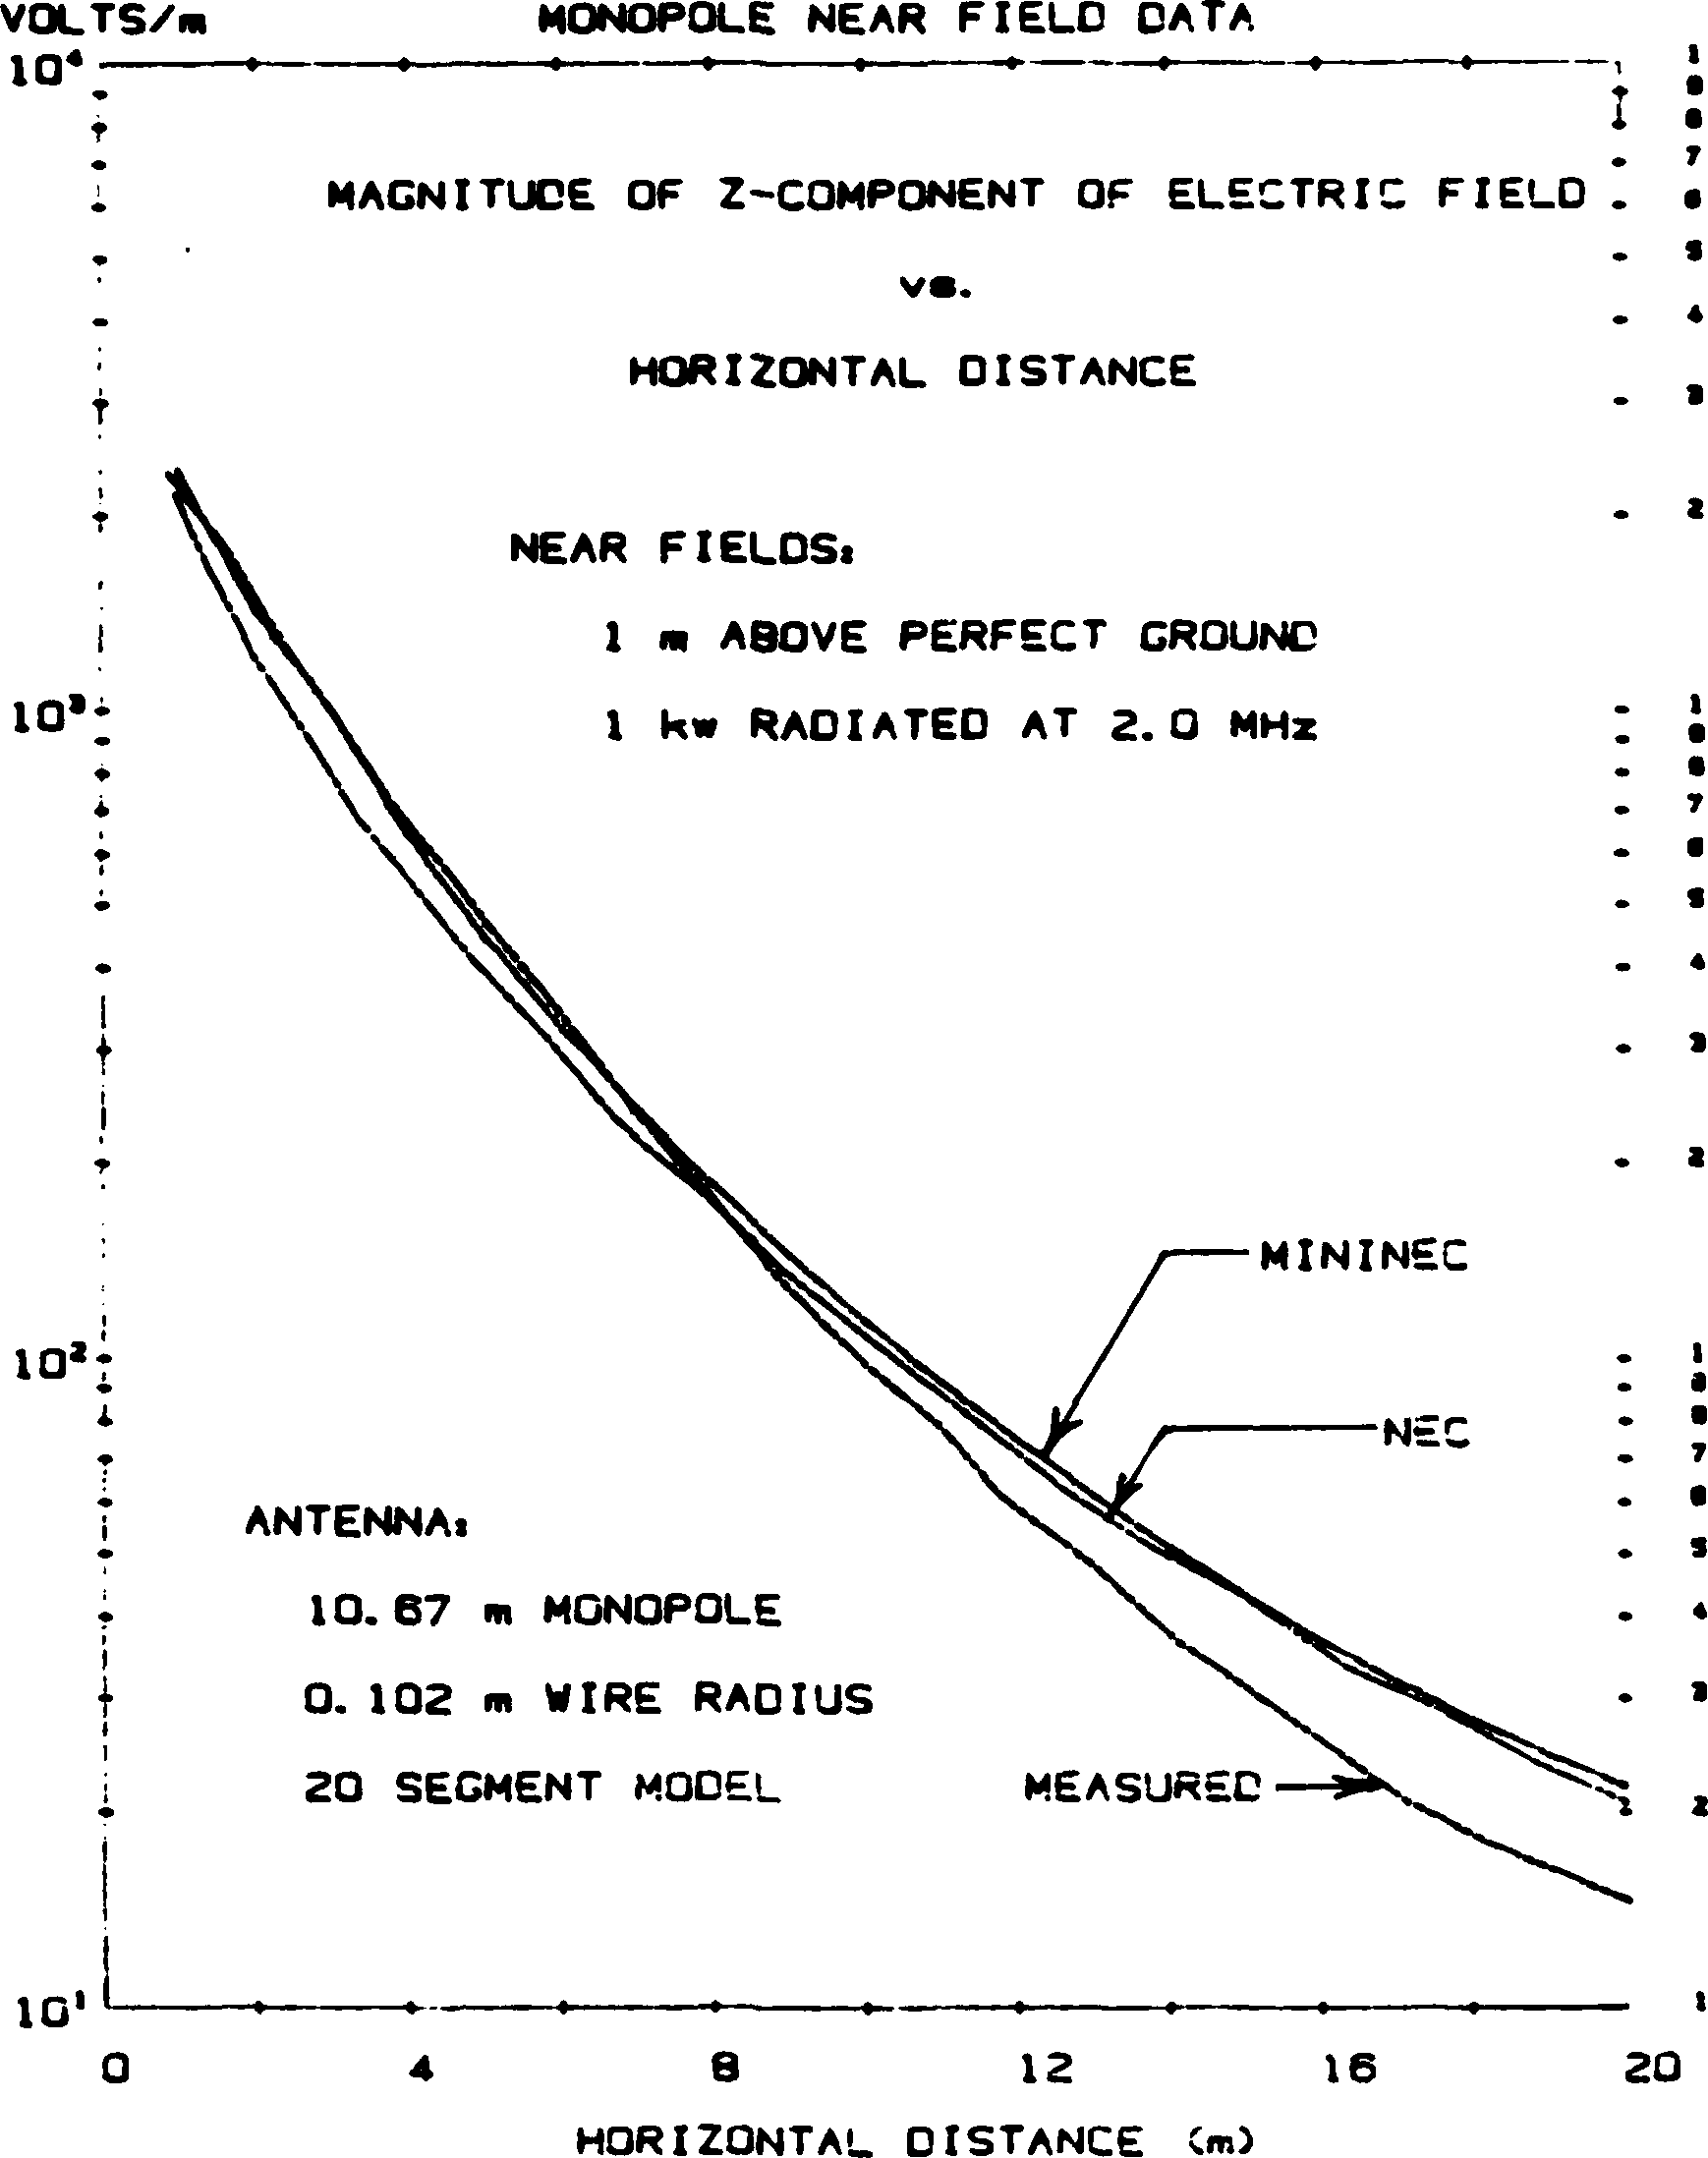
\includegraphics{fig32.eps}}
\caption{Comparison of near field data from MININEC and NEC to measurements}
\label{fig32}
\end{figure}

\begin{figure}[htb]
\centerline{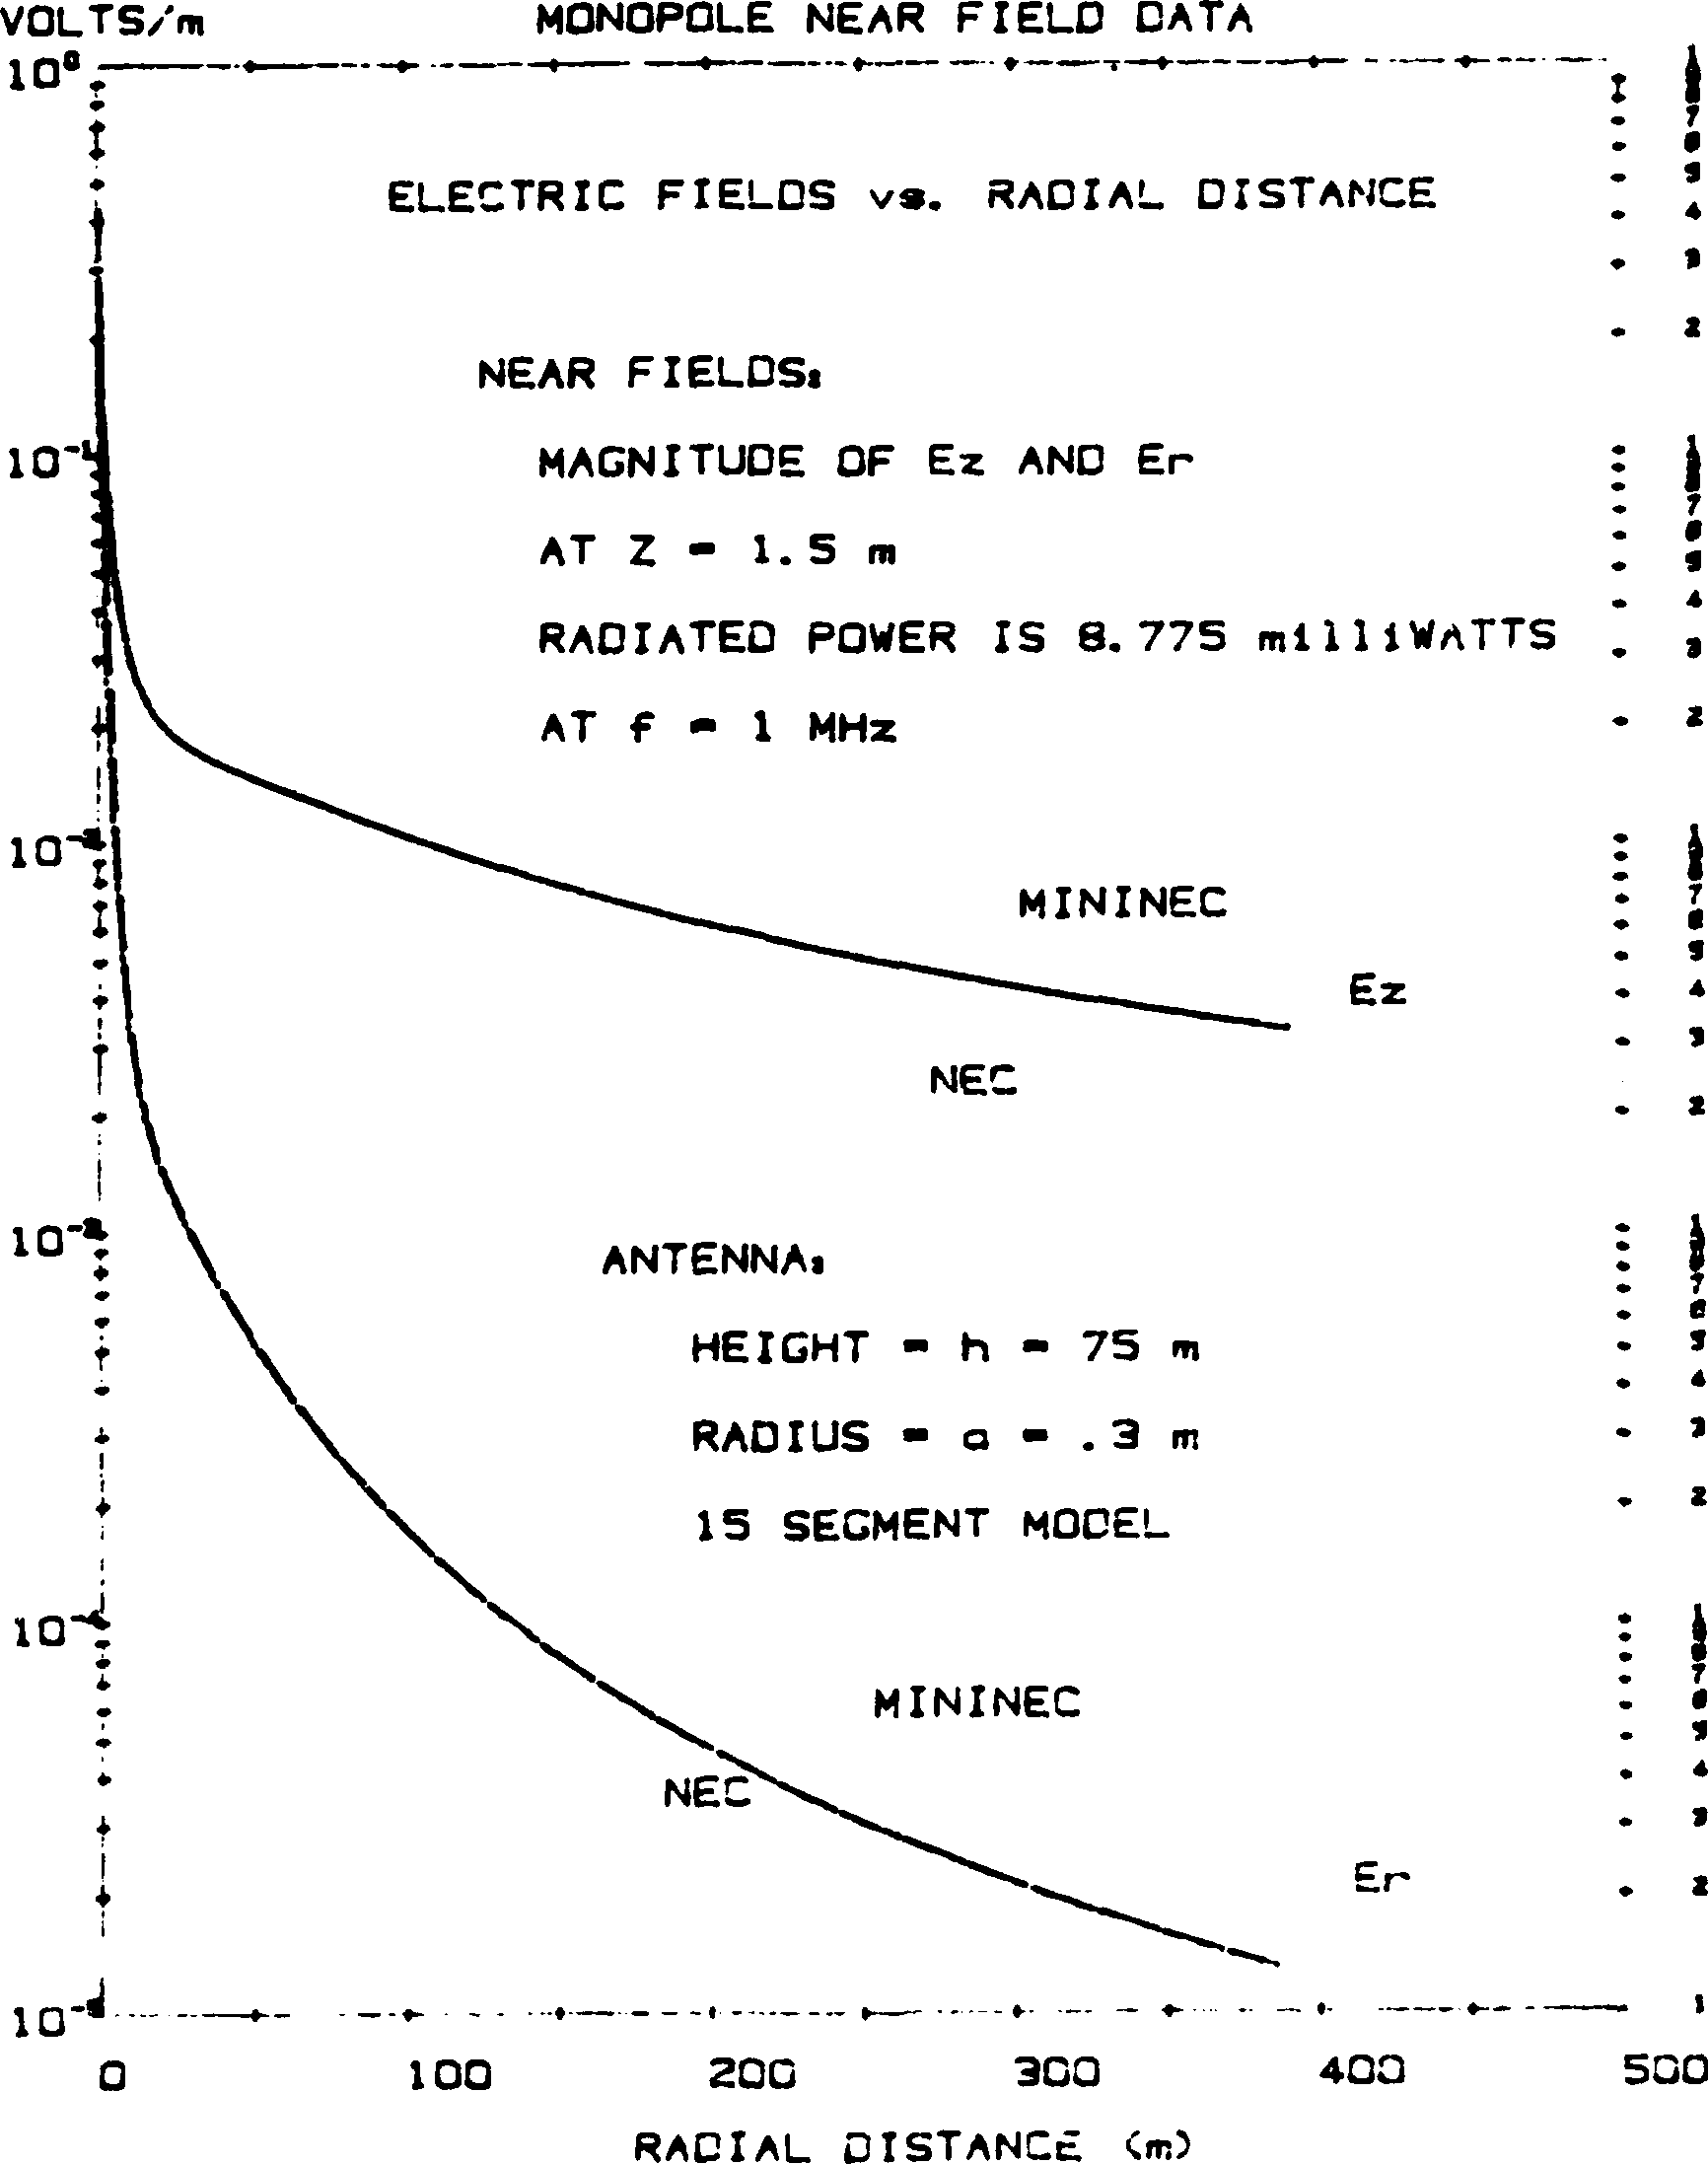
\includegraphics{fig33.eps}}
\caption{Near electric fields of a quarterwave monopole computed by
MININEC and NEC}
\label{fig33}
\end{figure}

\begin{figure}[htb]
\centerline{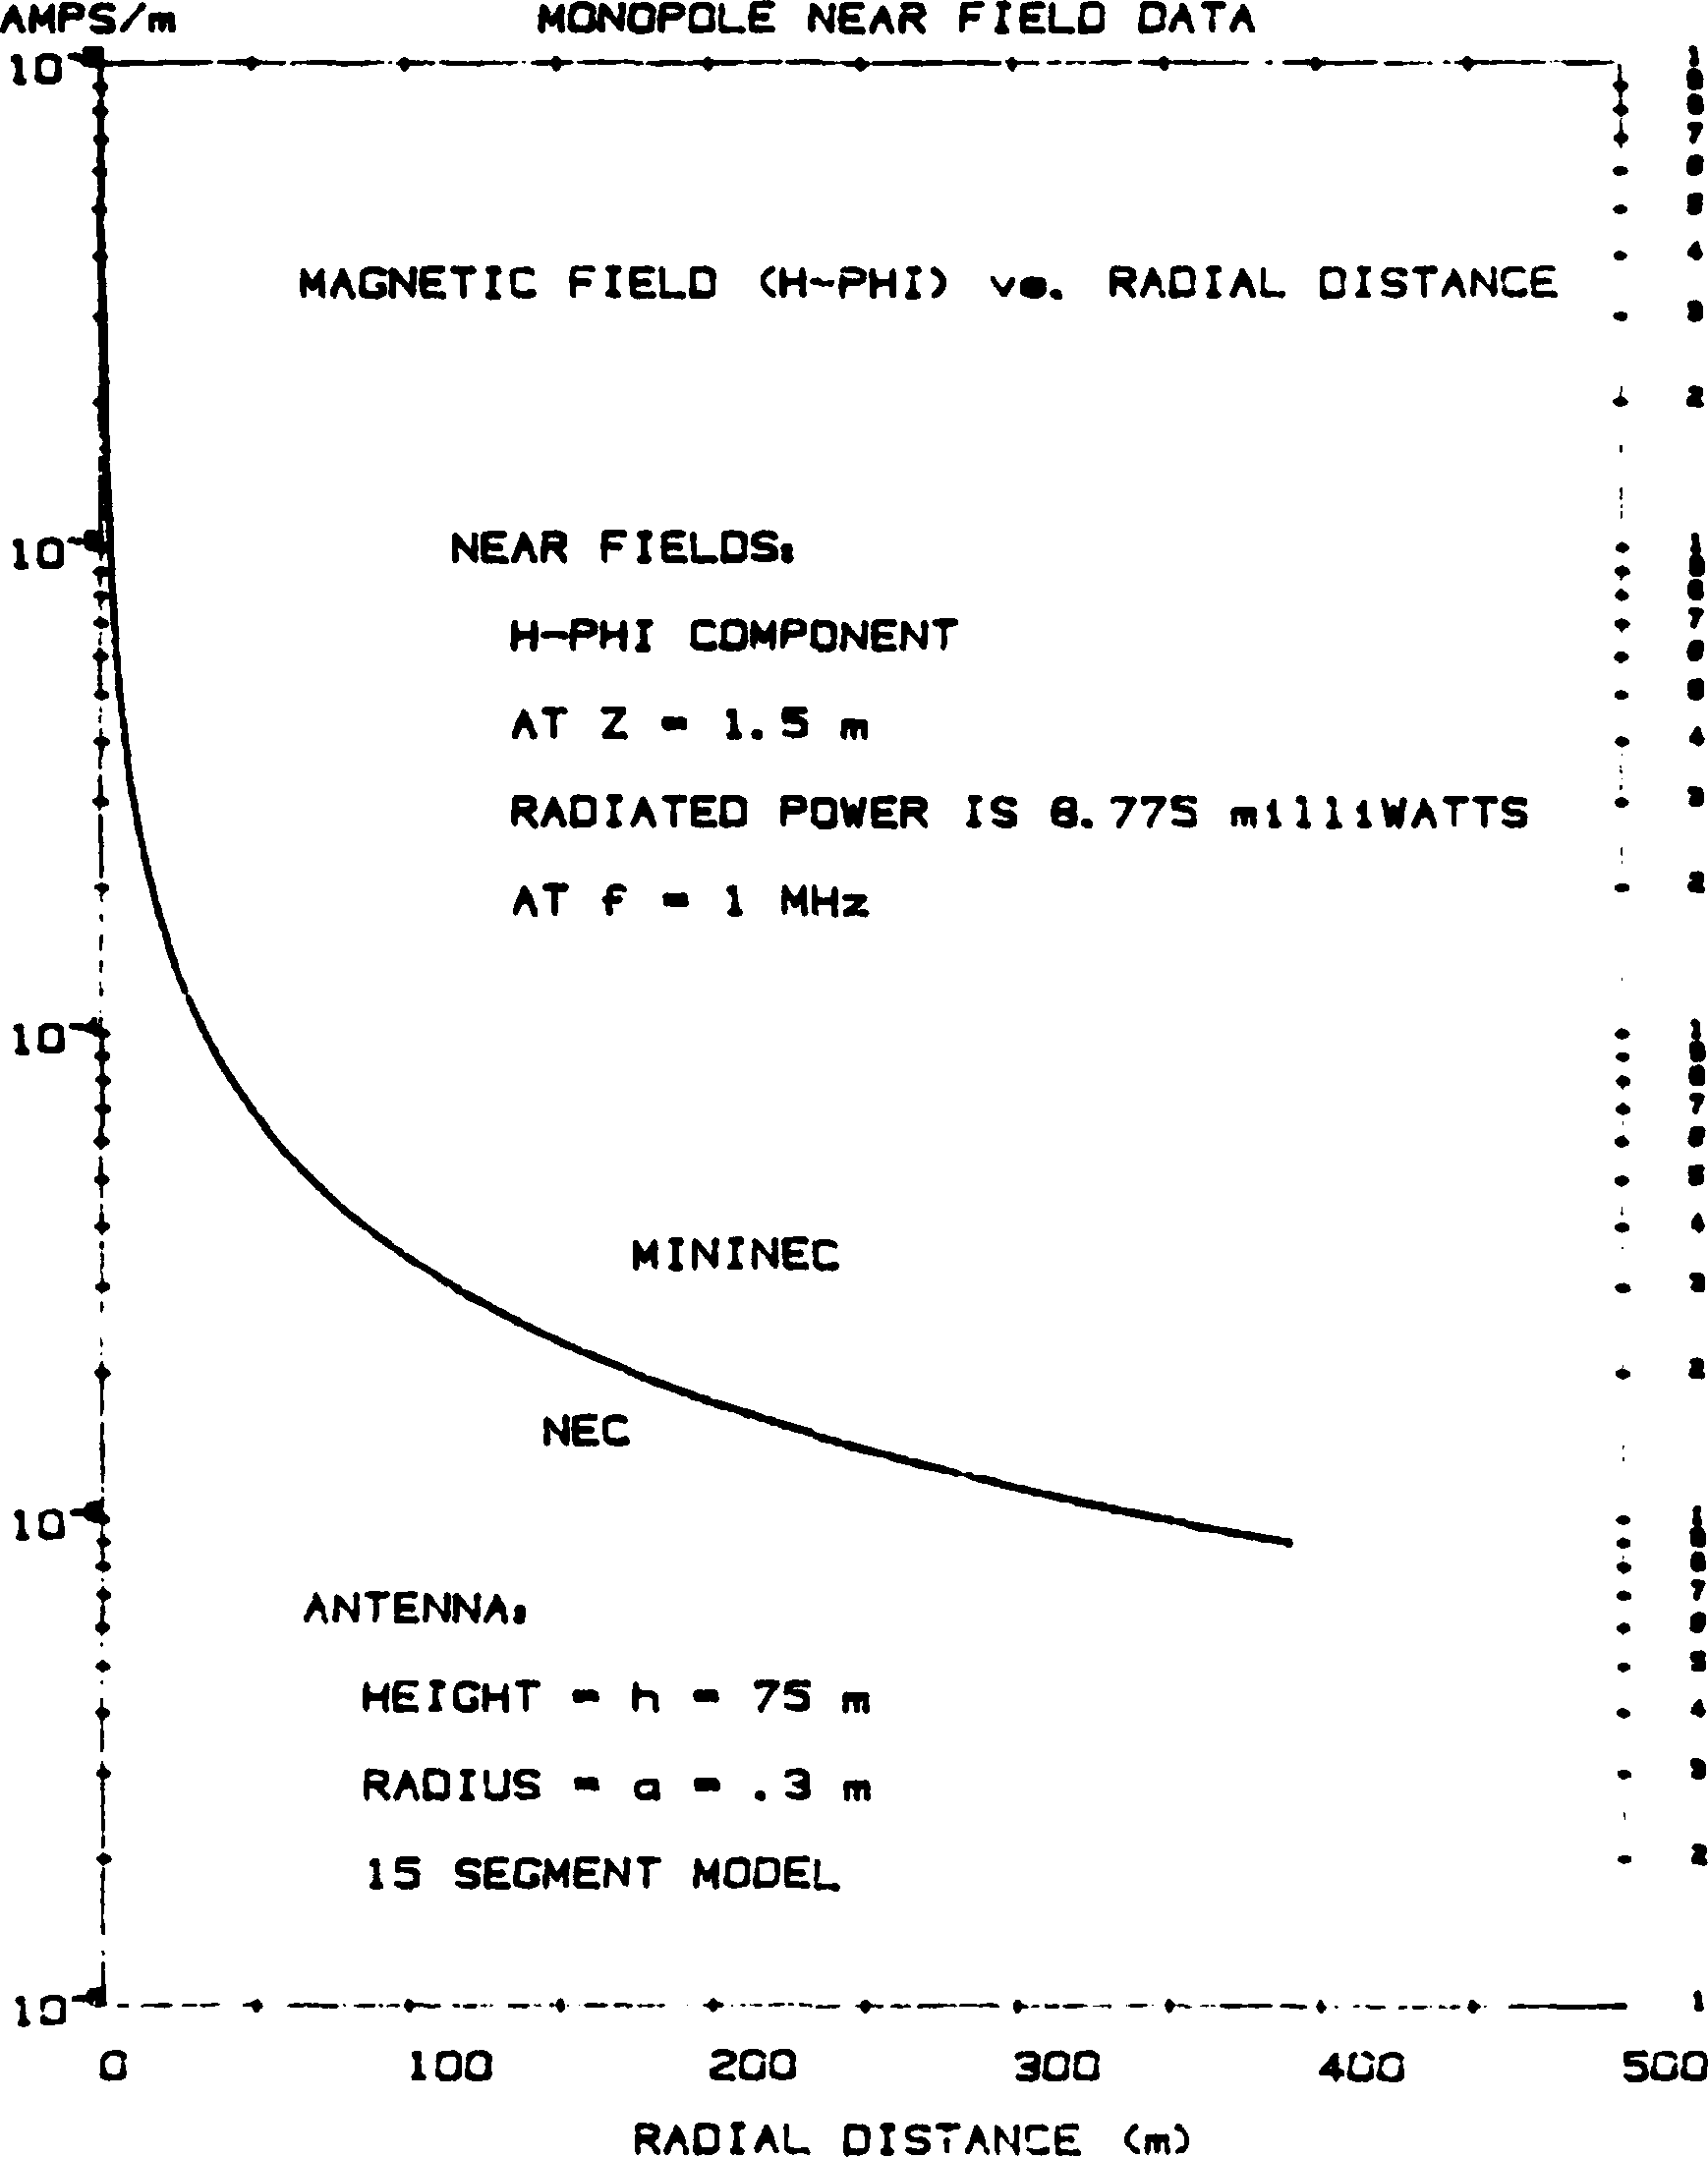
\includegraphics{fig34.eps}}
\caption{Near magnetic fields of a quarterwave monopole computed by
MININEC and NEC}
\label{fig34}
\end{figure}

\begin{sidewaysfigure}[htb]
\centerline{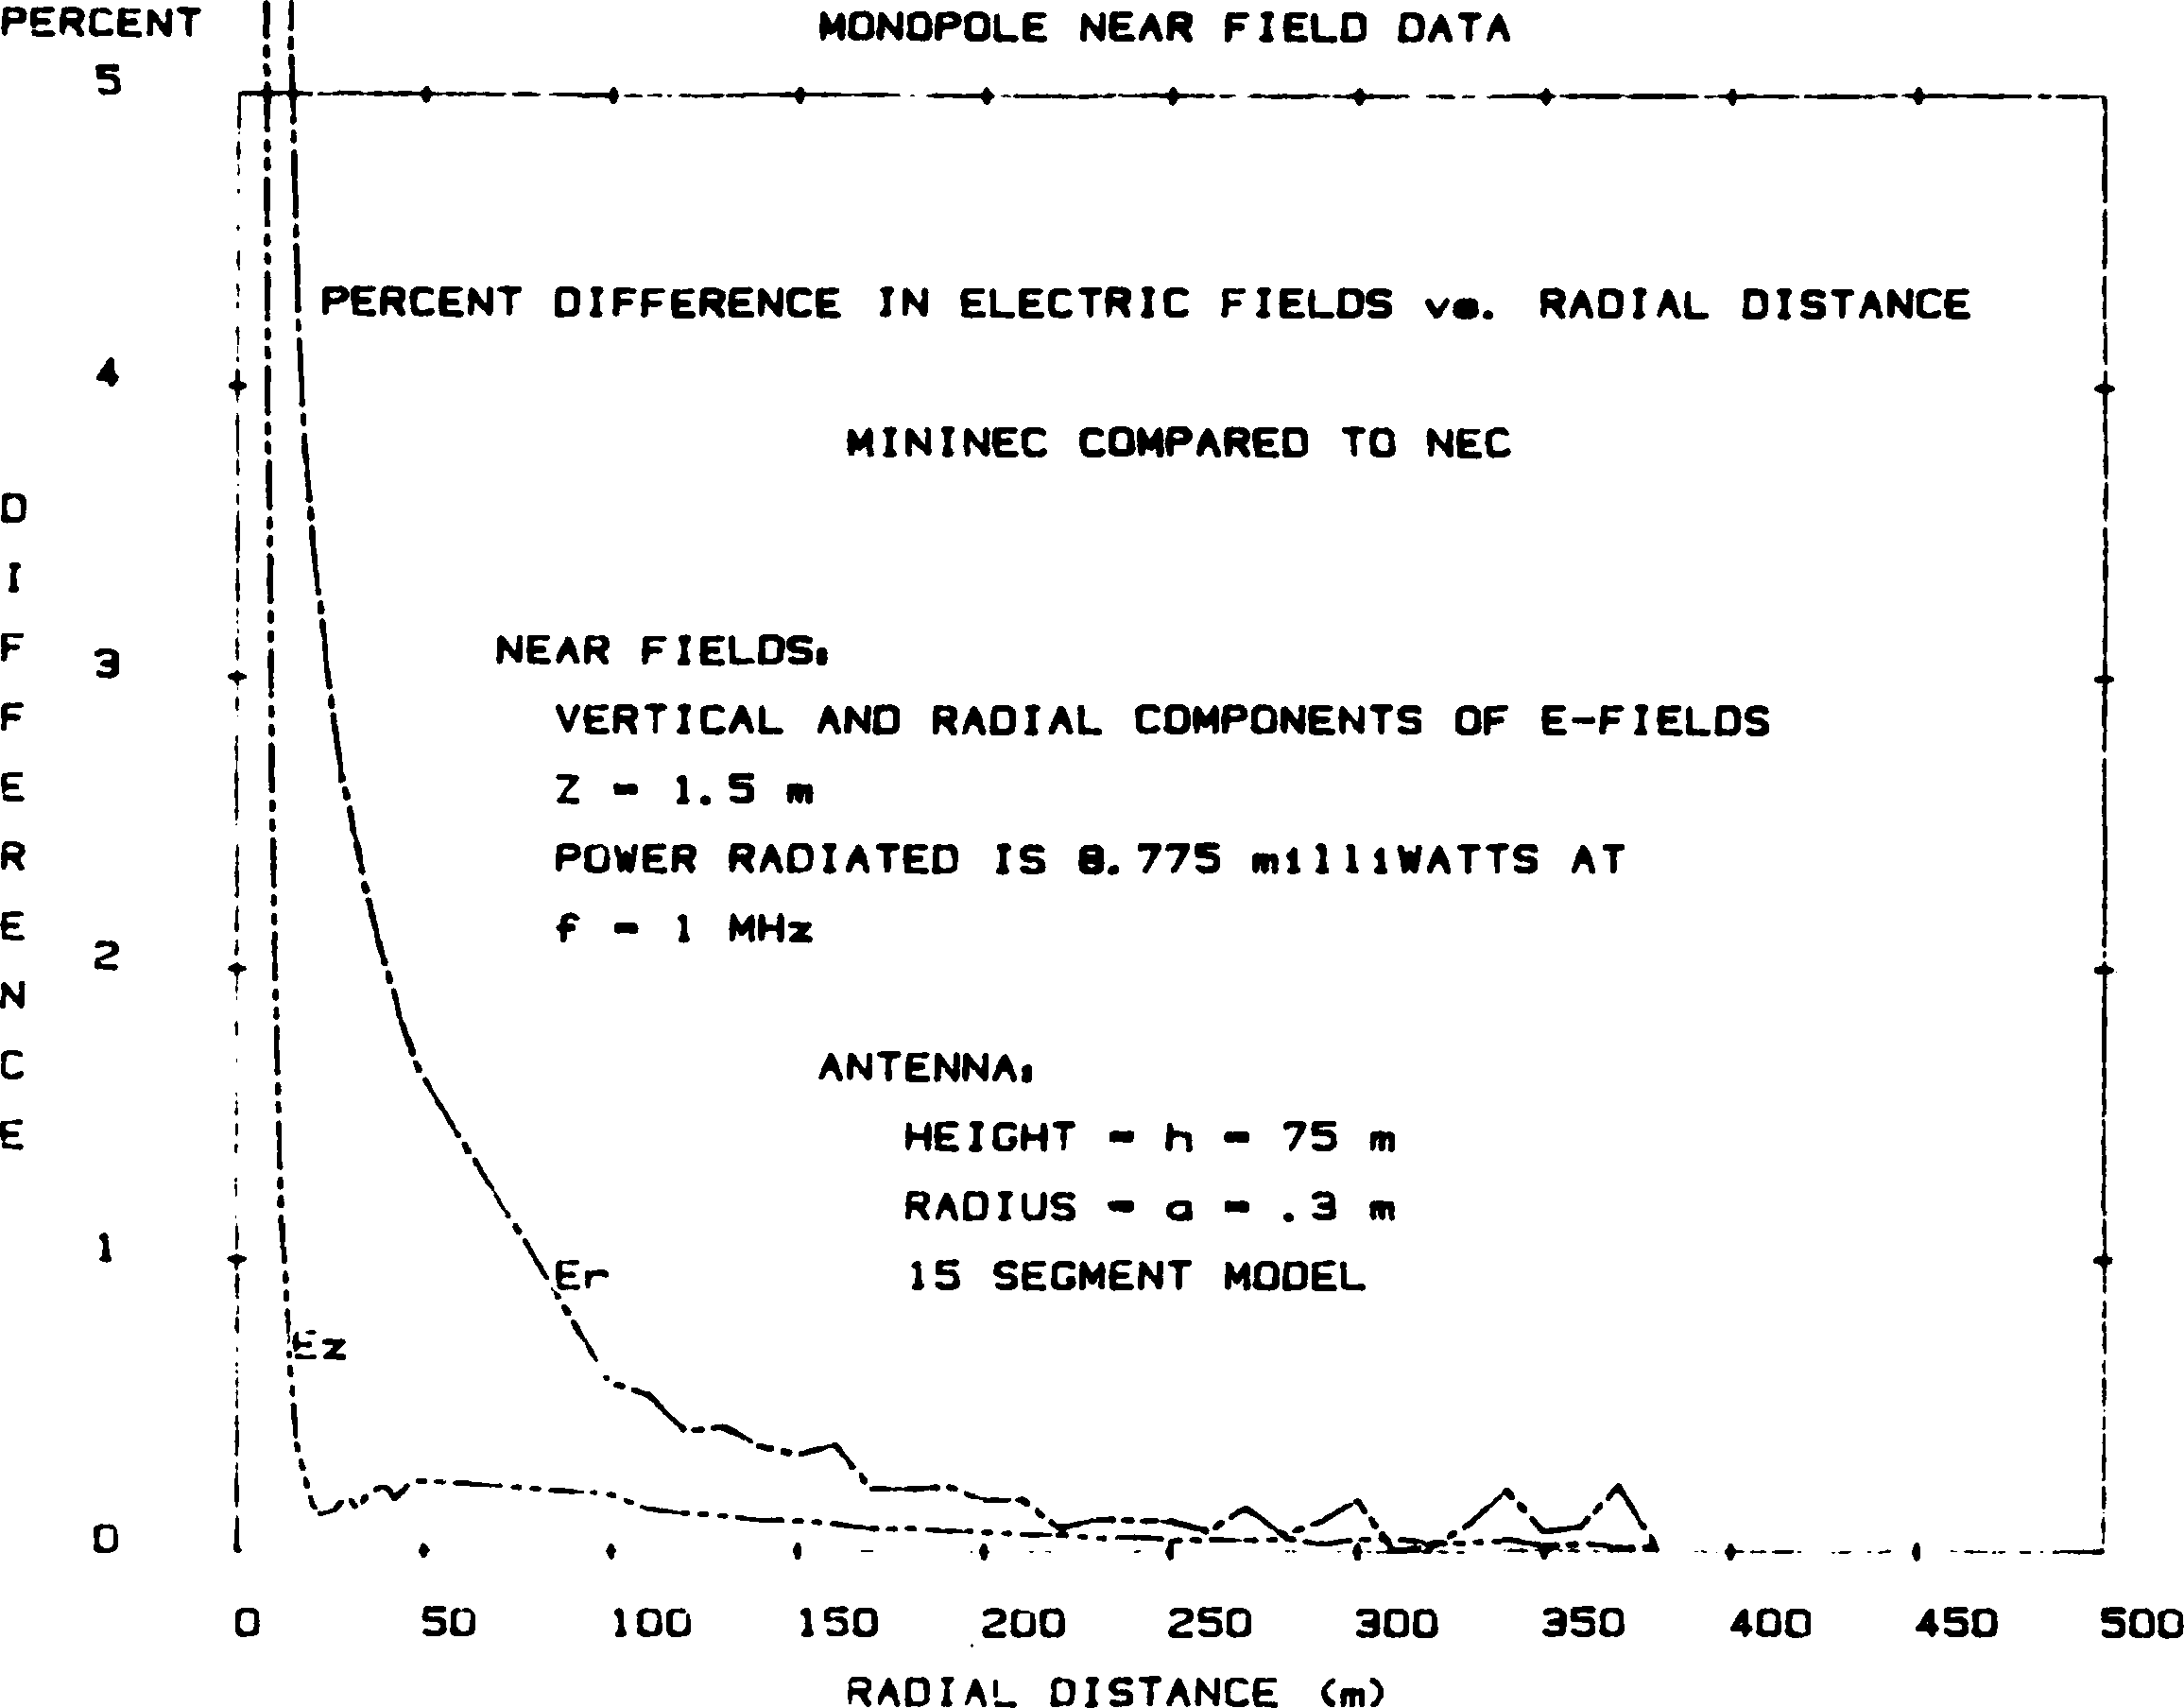
\includegraphics{fig35.eps}}
\caption{Percent difference between MININEC and NEC for the near field
data in Figures~\ref{fig33} and~\ref{fig34} (Part~1)}
\label{fig35}
\end{sidewaysfigure}

\begin{sidewaysfigure}[htb]
\centerline{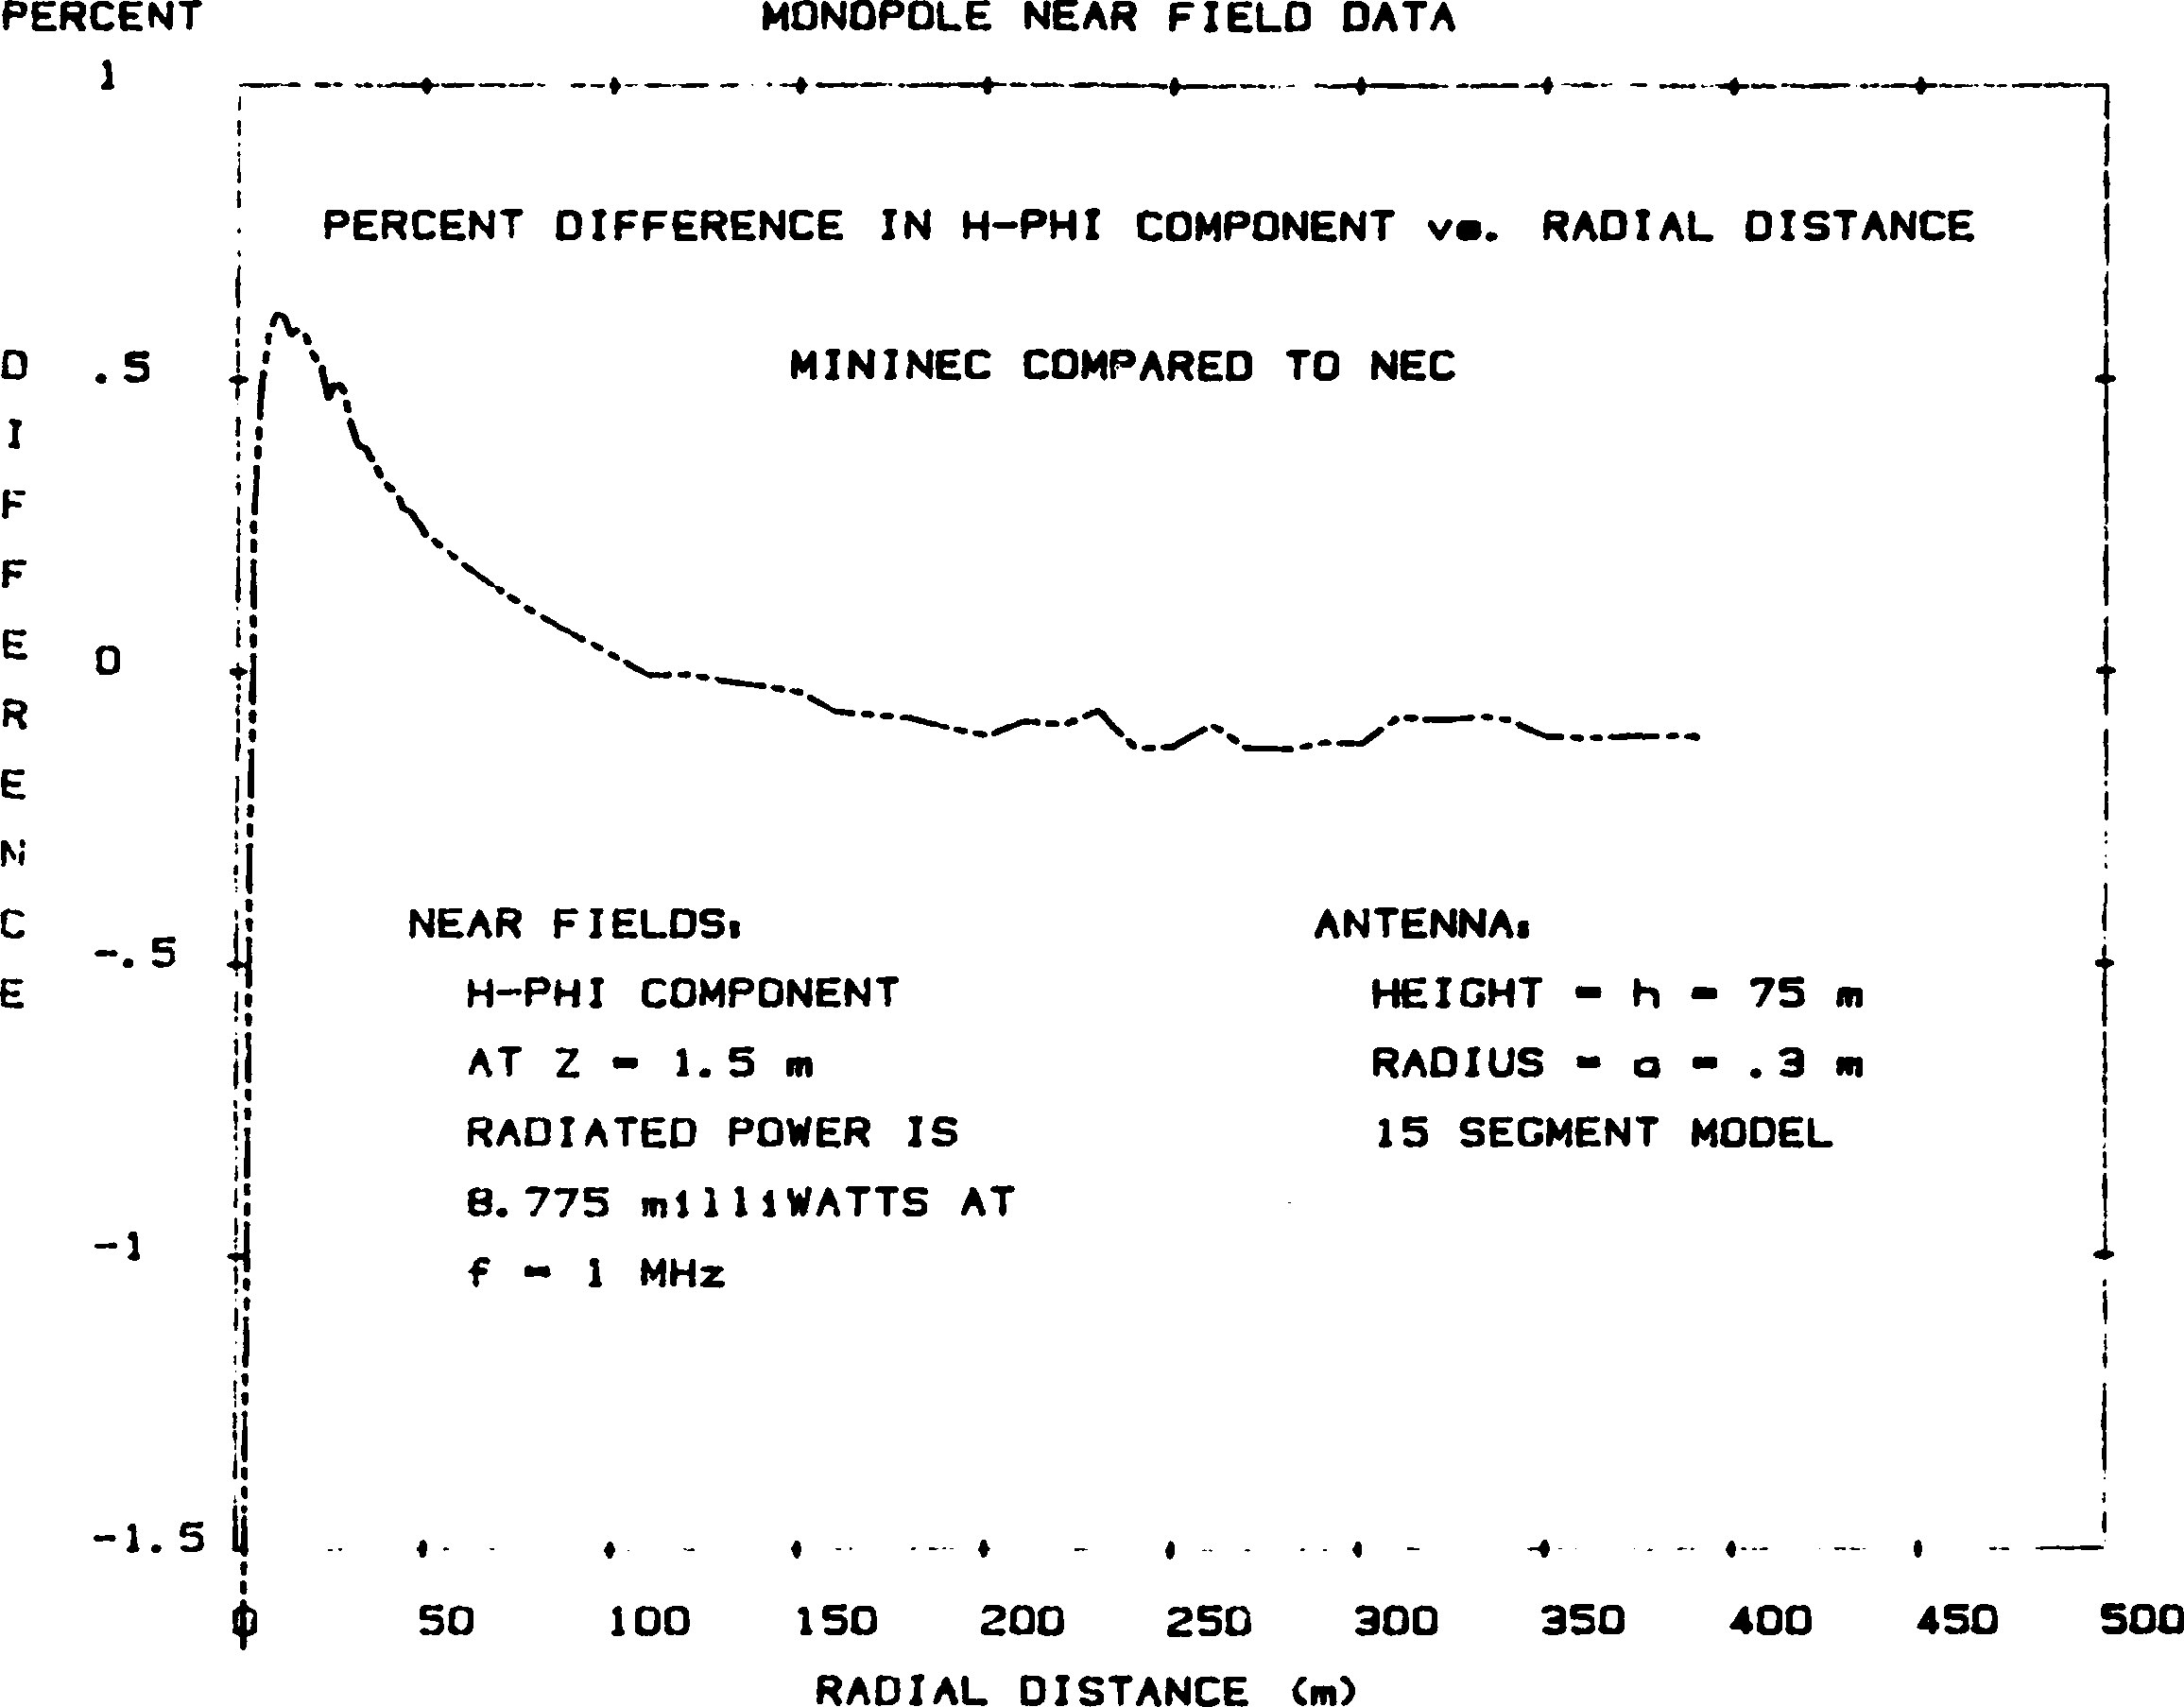
\includegraphics{fig36.eps}}
\caption{Percent difference between MININEC and NEC for the near field
data in Figures~\ref{fig33} and~\ref{fig34} (Part~2)}
\label{fig36}
\end{sidewaysfigure}

\begin{figure}[htb]
\centerline{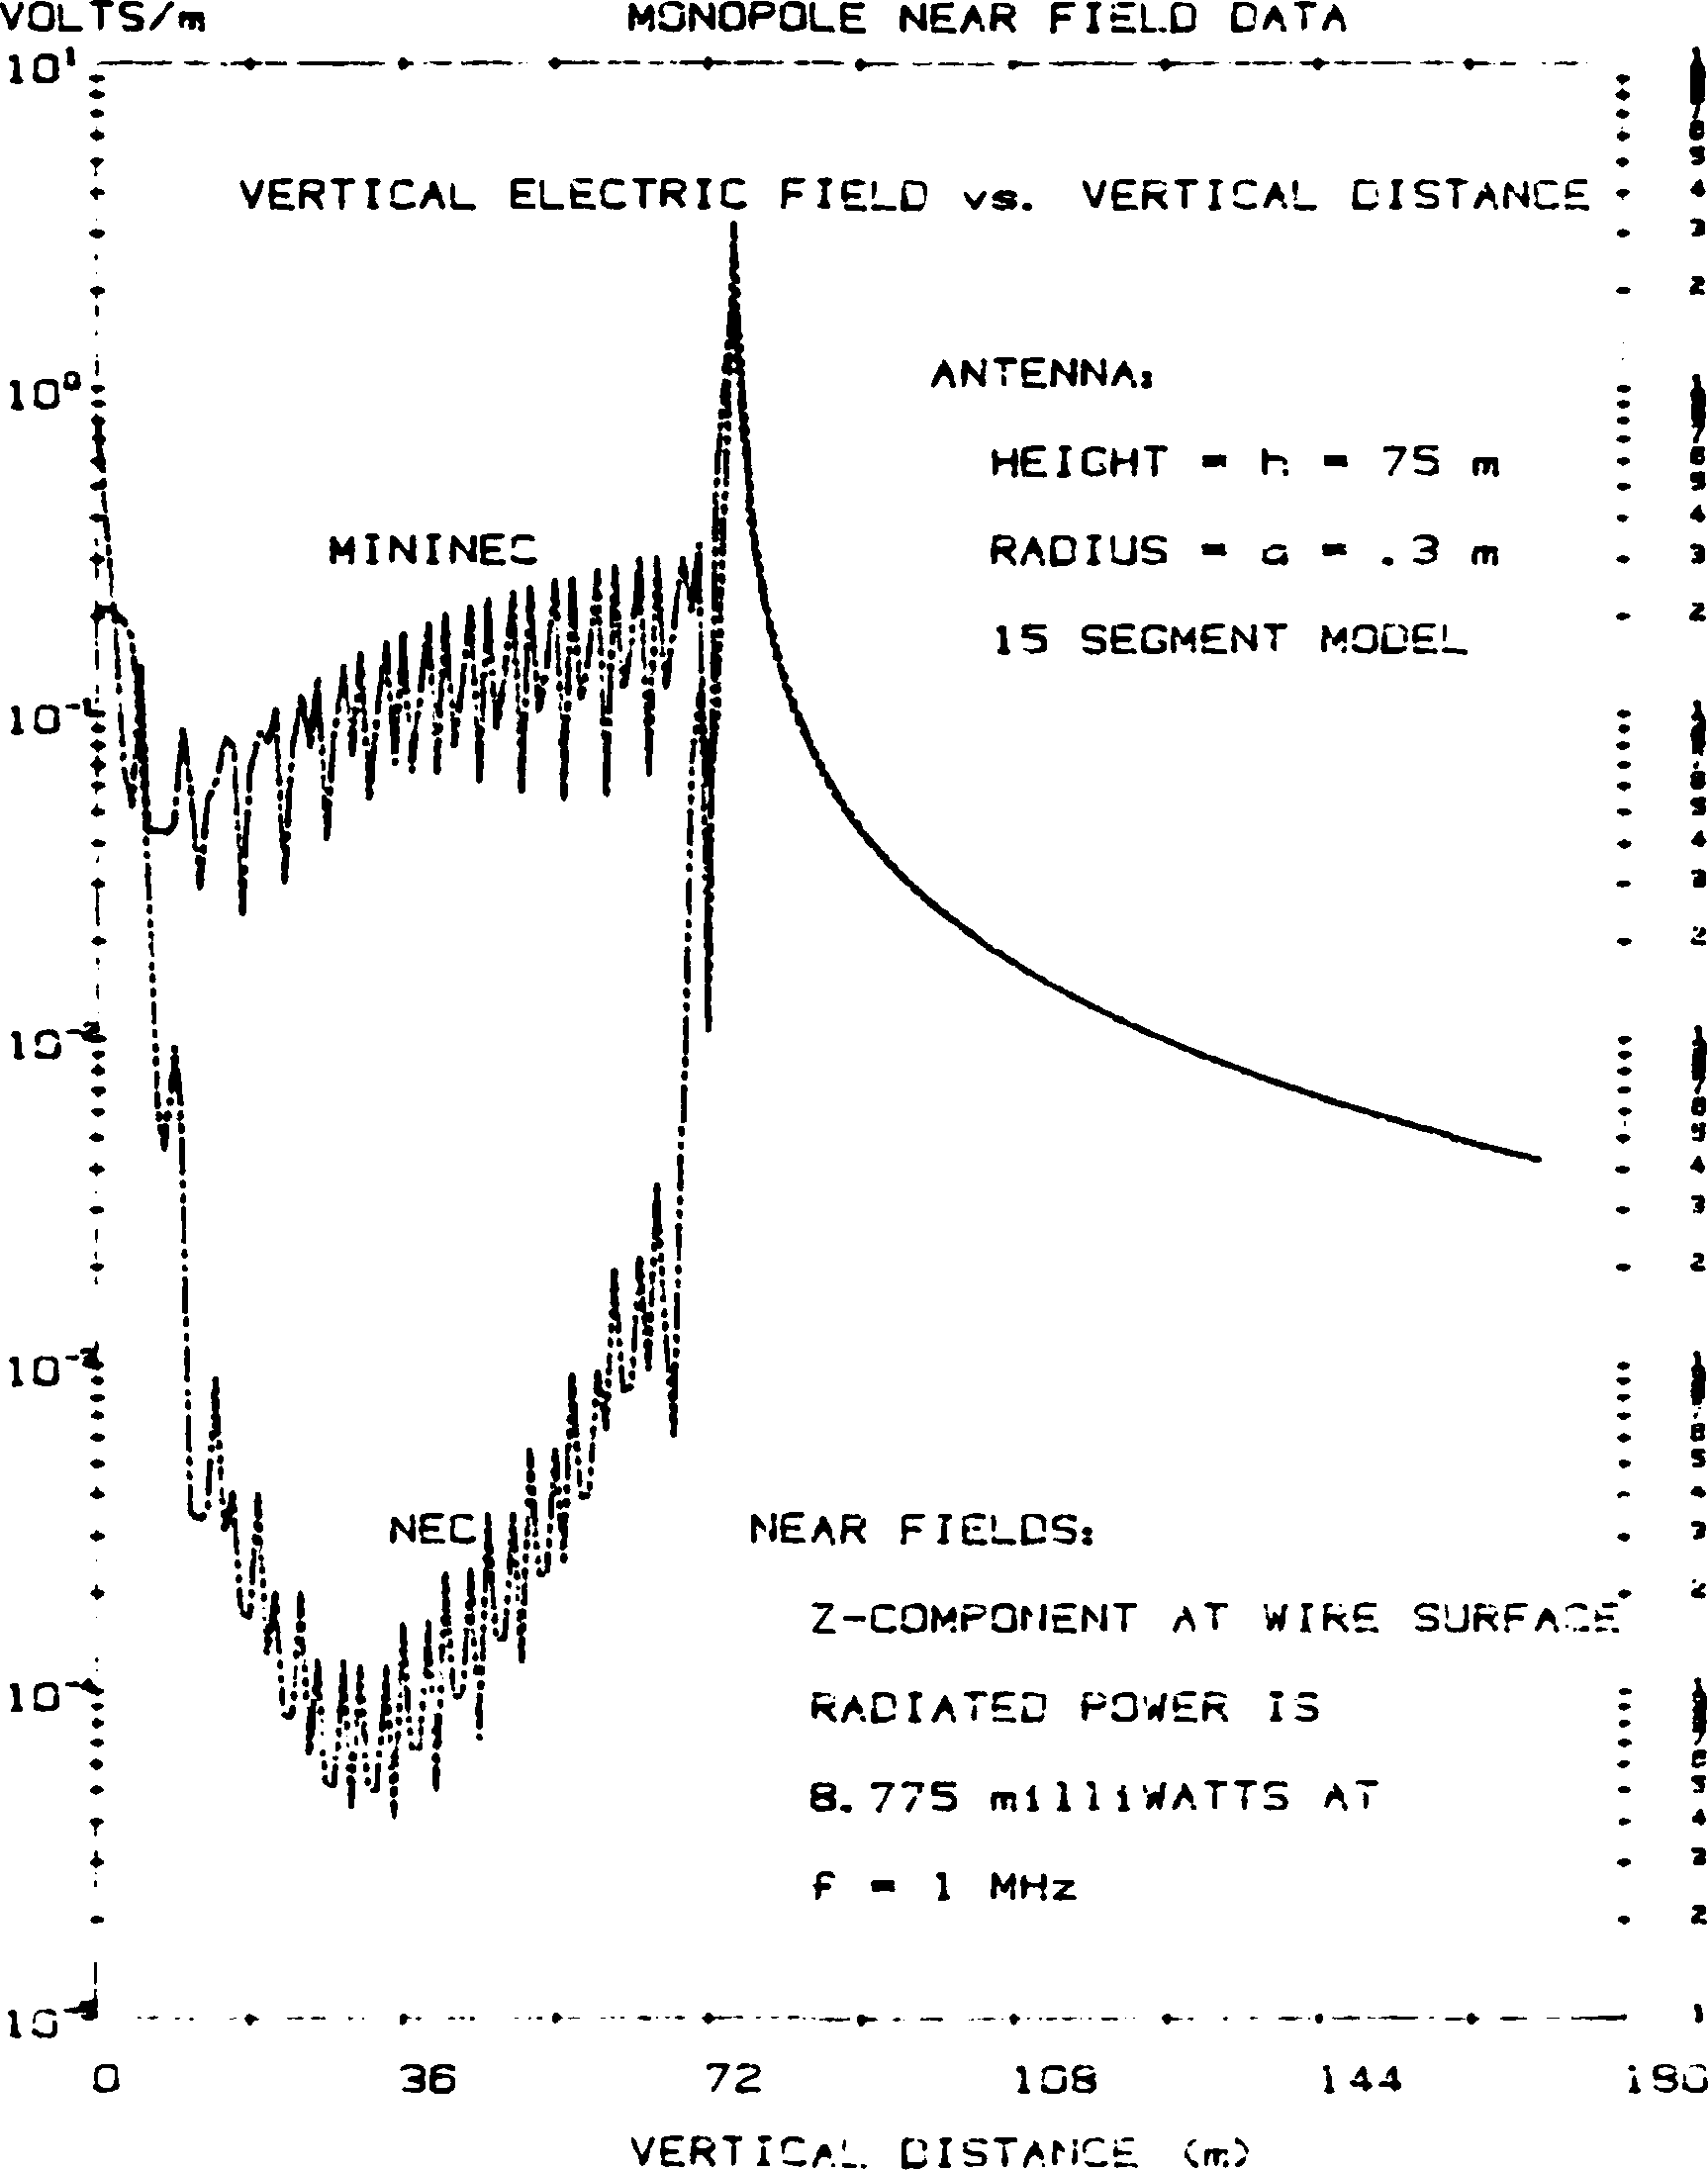
\includegraphics{fig37.eps}}
\caption{Vertical component of the electric field at one radius distance
for a quarterwave monopole}
\label{fig37}
\end{figure}

\begin{figure}[htb]
\centerline{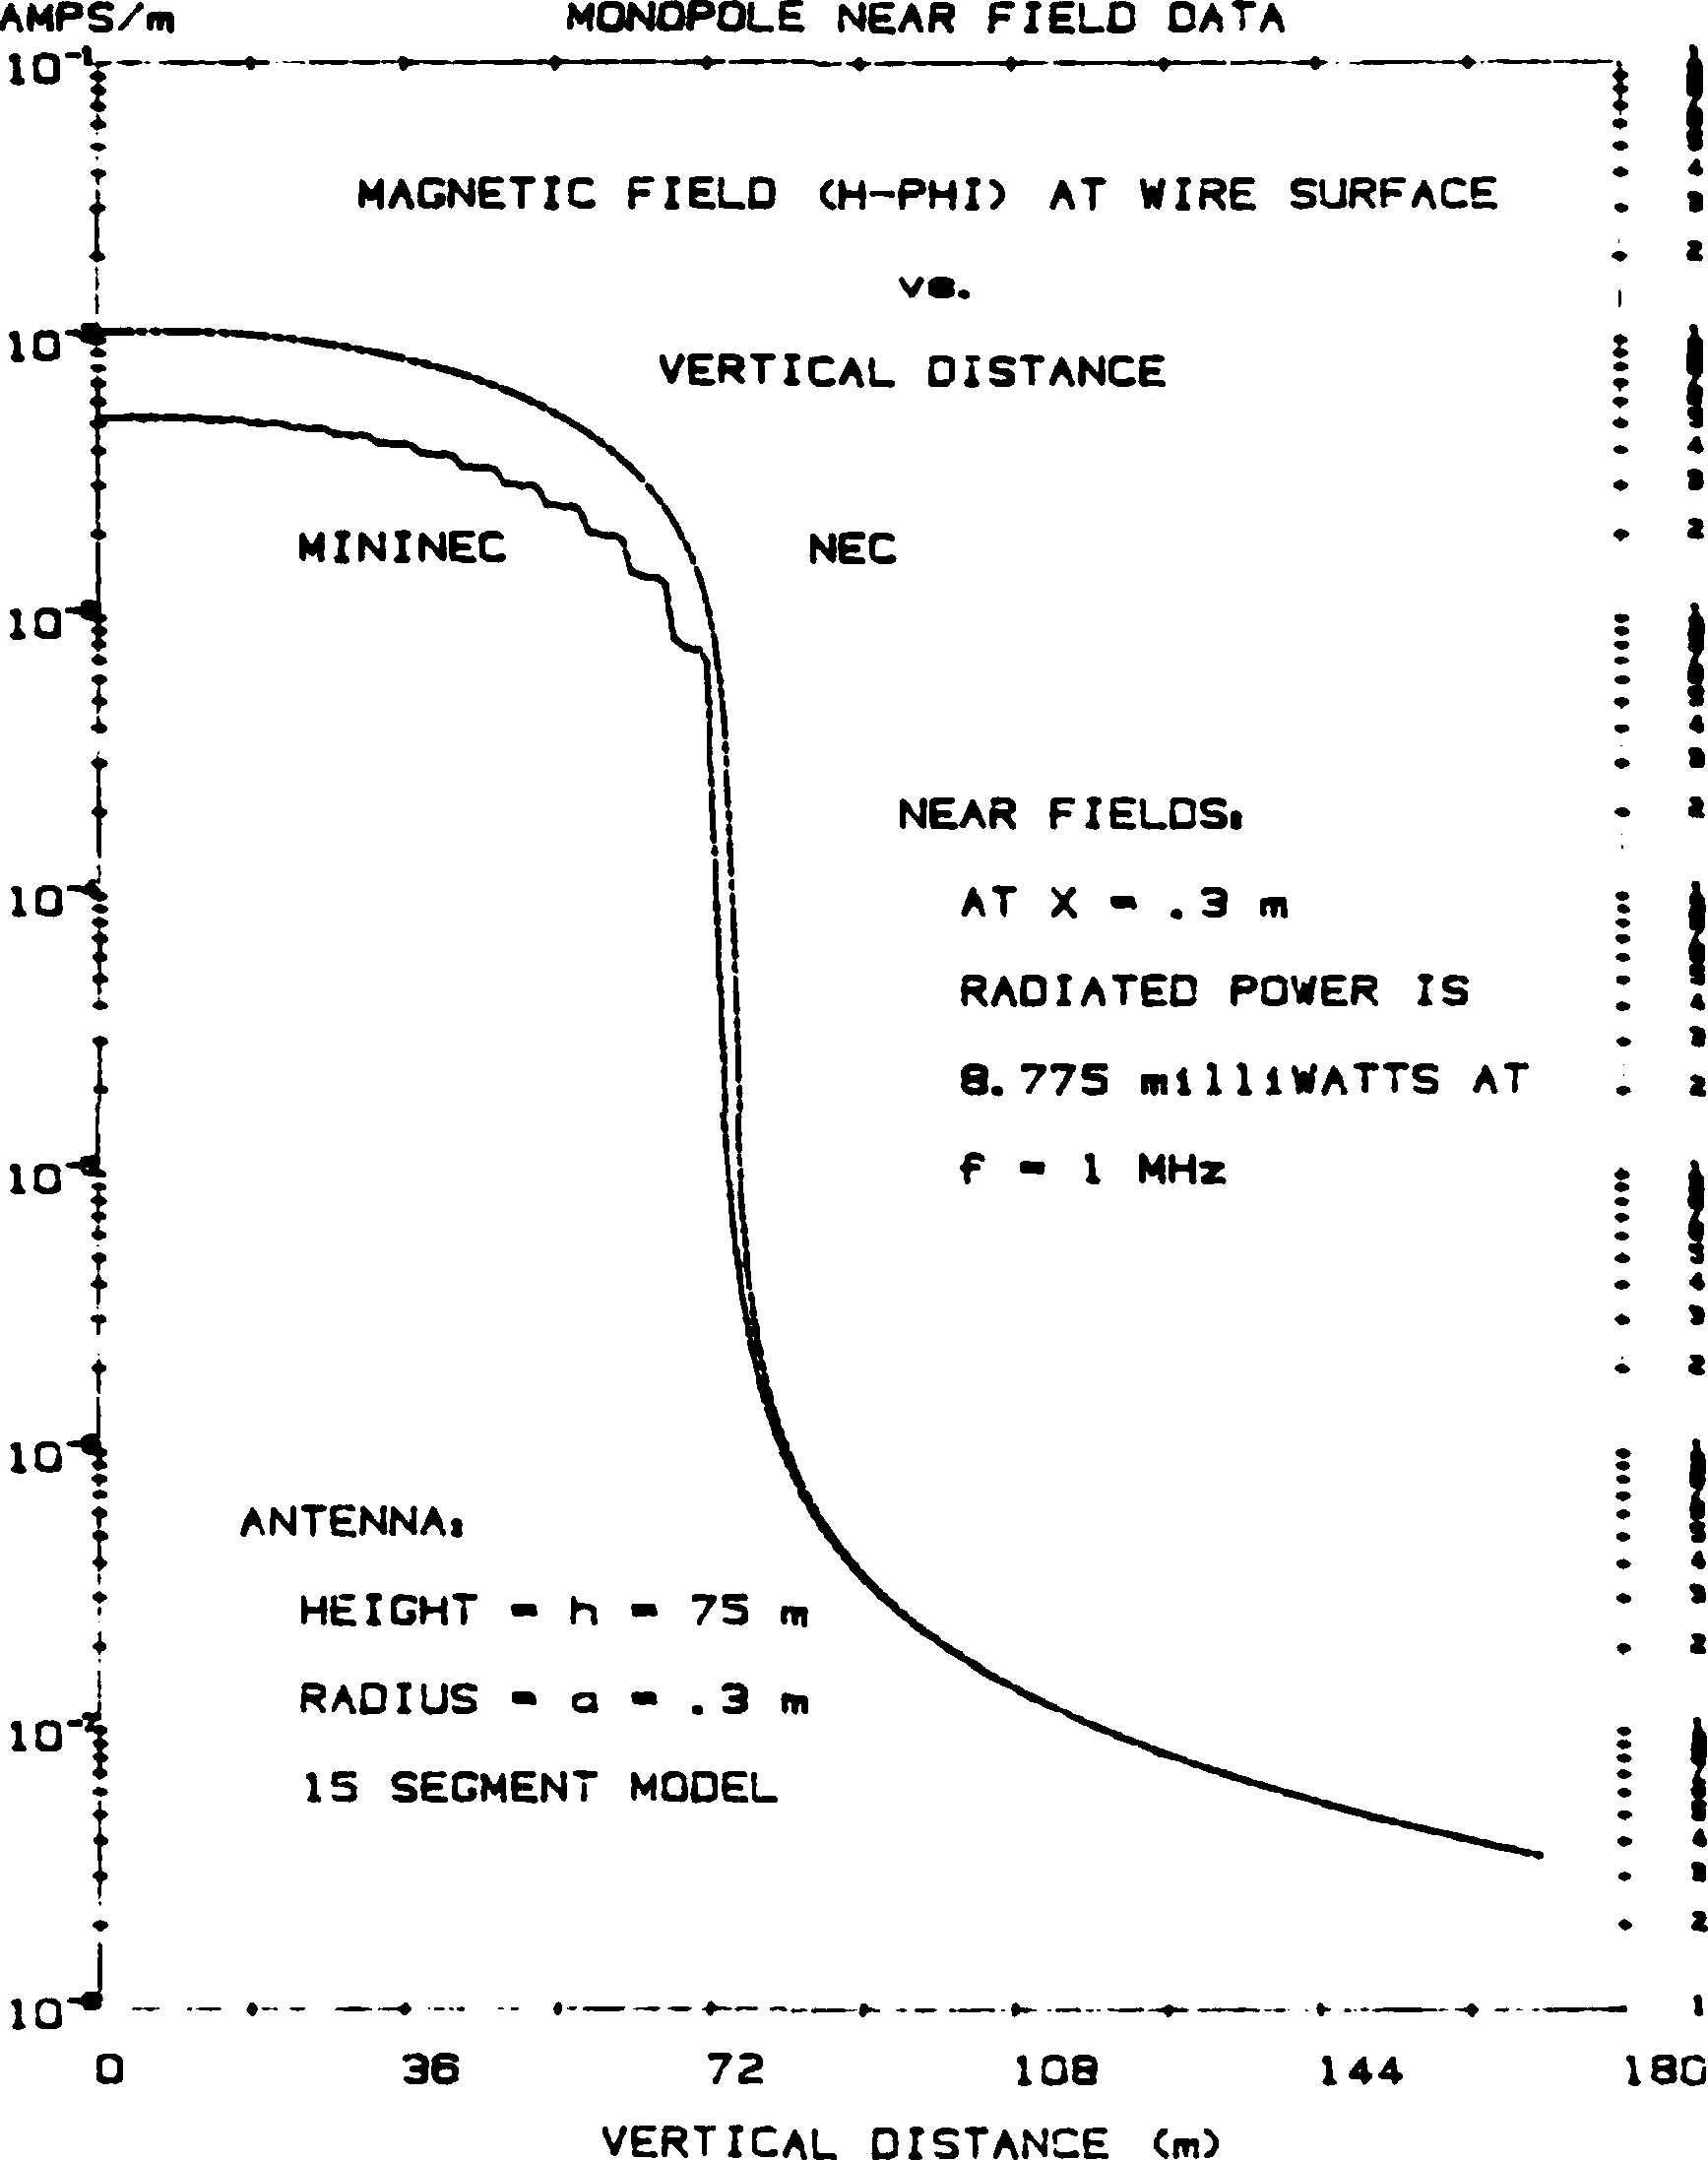
\includegraphics{fig38.eps}}
\caption{Horizontal component of the electric field at one radius distance
for a quarterwave monopole}
\label{fig38}
\end{figure}

\begin{figure}[htb]
\centerline{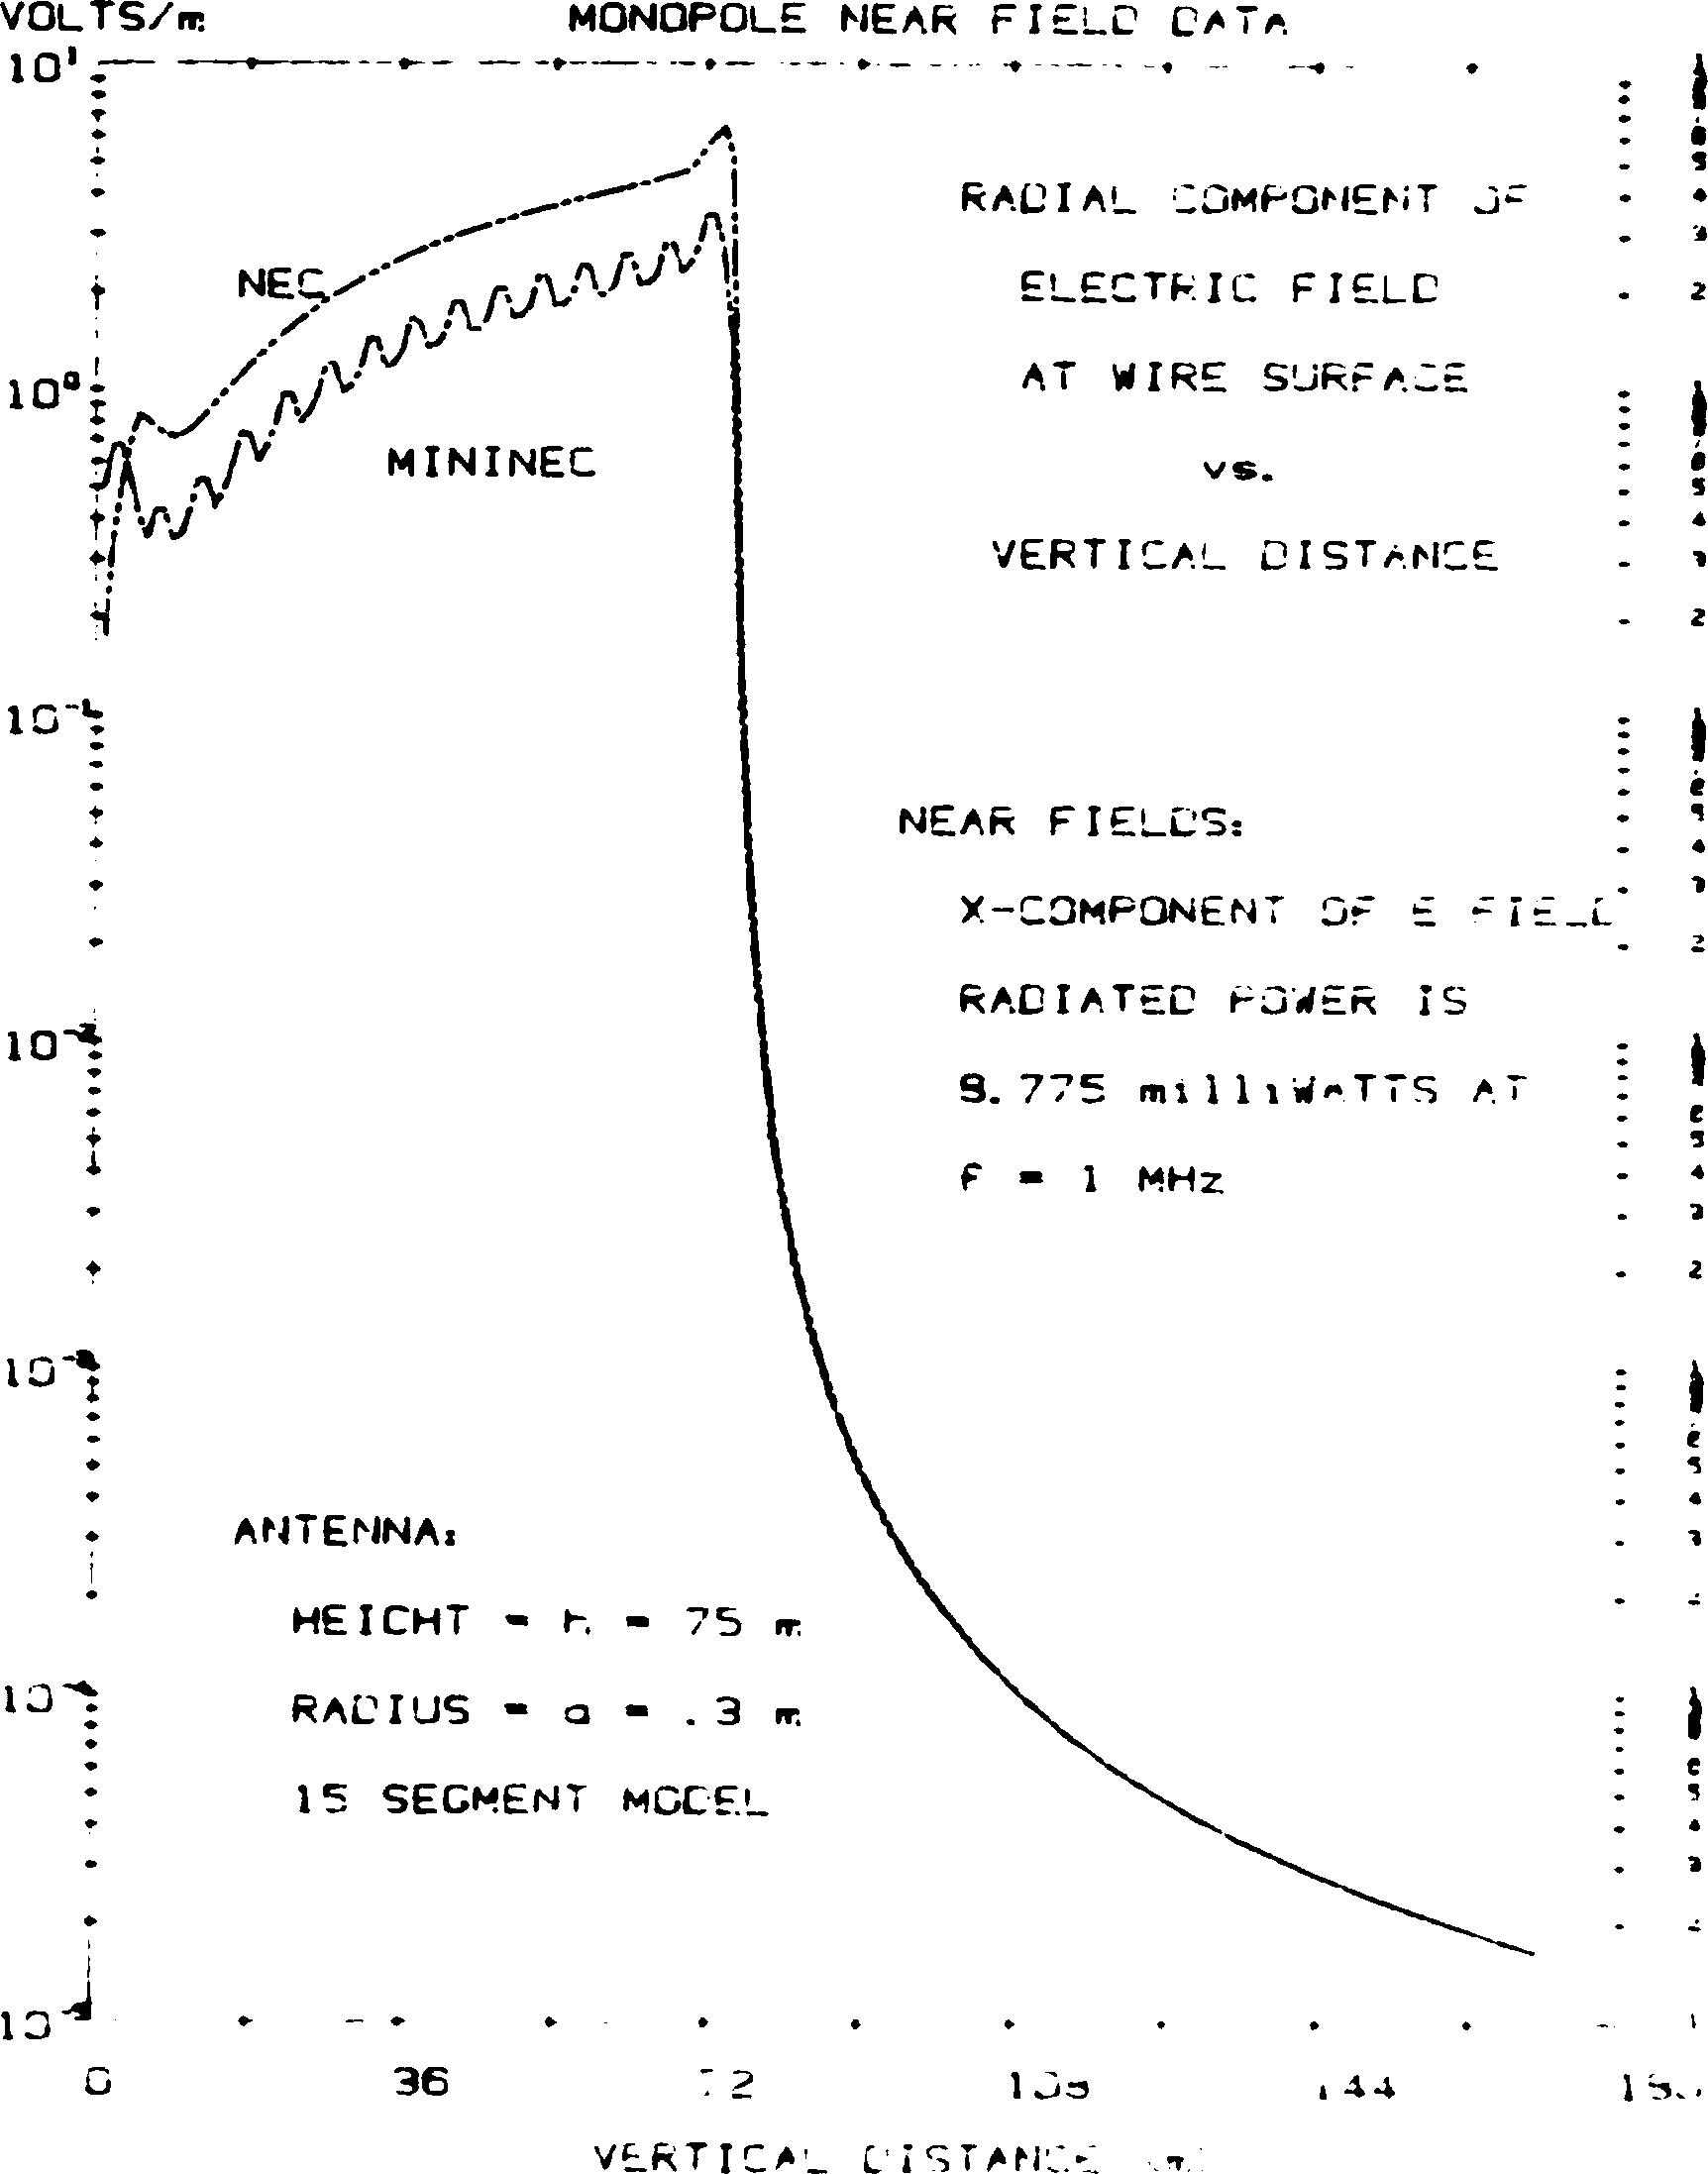
\includegraphics{fig39.eps}}
\caption{Phi-component of the magnetic field at one radius distance
for a quarterwave monopole}
\label{fig39}
\end{figure}

\begin{figure}[ht]
\begin{center}
Radiation Resistance and Gain for Dipole Antennas
\end{center}
\begin{tabular}{lcllcllcl}
\multicolumn{3}{c}{MININEC Data}       &
\multicolumn{3}{c}{Schelkunoff Data}   &
\multicolumn{3}{c}{Jasik Data}         \\
\multicolumn{3}{l}{Wire Stub:}         &
\multicolumn{3}{l}{Current Element:}   &
\multicolumn{3}{l}{Very Short Dipole:} \\
N & = & 2 segments & \multicolumn{3}{l}{constant current} \\
l & = & length = $.02\lambda$ & l & = & $.02\lambda$      \\
a & = & radius = $.001\lambda$                            \\
Z & = & $.0790-\jj3388$ ohms & R & = & $80s^2(1/\lambda)^2 = .3158$ ohms \\
G & = & 1.754 dB & G & = & 1.761 dB & G & = & 1.76 dB     \\
\\
\multicolumn{3}{l}{Half Wave Dipole:} &
\multicolumn{3}{l}{Half Wave Dipole:} &
\multicolumn{3}{l}{Half Wave Dipole:} \\
N & = & 30 & \multicolumn{3}{l}{cosine current} \\
l & = & .5~m & l & = & $.5\lambda$ \\
a & = & 0.00001~m \\
f & = & 293 MHz \\
Z & = & 72.21+\jj.6485 ohms &
R & $\rightarrow$ & \multicolumn{4}{l}{73.13 ohms as $a/\lambda\rightarrow0$} \\
G & = & 2.13 dB   & G & = & 2.151 dB & G & = & 2.15 dB \\
  &   &           &   &   &          & \multicolumn{3}{l}{(Krauss: 2.14 dB)} \\
\multicolumn{3}{l}{Full Wave Dipole:} &
\multicolumn{3}{l}{Full Wave Dipole:} \\
N & = & 30        & \multicolumn{3}{l}{cosine current distribution} \\
l & = & 1 m       & l & = & $1\lambda$ \\
a & = & .00001 m  & l & = & $0.00001\lambda$ \\
f & = & 285.3 MHz & R & = &
    \multicolumn{4}{l}{$(276\log \lambda/{2a}) - 110l^2/199$} \\
Z & = & 6958-j26.51 ohms  &   & = & 7145 ohms \\
G & = & 3.63 dB   & G & = & 3.82 dB   \\
\end{tabular}
\begin{center}
Monopole Radiation Resistance and Gain\\\ \\
\begin{tabular}{ll}
\multicolumn{1}{c}{MININEC} & \multicolumn{1}{c}{Jasik} \\
N${}=15$ segments            & ``quarter wave dipole    \\
h${}=.25$ m                  & above perfect ground''   \\
a${}=.00001$ m               &                          \\
f${}=293$ MHz                &                          \\
Z${}=36.10+\jj.3352$ ohms    &                          \\
G${}=5.145$ dB               & G${}=5.15$ dB            \\
\end{tabular}
\end{center}
\caption{Comparison of MININEC impedance and gain data to classical
values given by Schelkunoff and Jasik.}
\label{fig40}
\end{figure}
\afterpage\clearpage

Figure~\ref{fig32} shows a comparison of MININEC and NEC and to
measurements. The data are the near electric fields of a 10.67-meter
monopole over a good conducting ground screen at 2~MHz. The fields are
for 1~KW radiated power. The measurements were made using an E-field
sensor (EFS-1) manufactured by Instruments for Industry
\cite{r21}. The NEC data are from a single precision version
(NEC-1) running on a VAX 11780 computer. The agreement between both
codes and the measurements is acceptable over the range shown. The
accuracy of the measurements is 5 to 10\%, with the greatest error
occurring for distances of 10 meters and greater, due to the effects of
nearby structures. The differences between NEC and MININEC are due in
part because the NEC data is from a single precision version.

Figures~\ref{fig33} and~\ref{fig34} are a comparison of MININEC and NEC
near field data for a quarter wave monopole over perfect ground. The NEC
data are from a double precision version (NEC-3) running on a VAX 11780
computer. Figure~\ref{fig33} gives the vertical and radial components of
the electric field and Figure~\ref{fig34} gives the phi-component of the
magnetic field. The MININEC data has been scaled to the power level of
the NEC data. The NEC and MININEC data are essentially identical.
Figures~\ref{fig35} and~\ref{fig36} show the percent difference between
the NEC and MININEC fields of Figures~\ref{fig33} and~\ref{fig34}. The
greatest difference occurs very close to the monopole within a segment
length.

If the near fields are calculated along the surface of the monopole, the
differences between MININEC and NEC are much more pronounced.
Figures~\ref{fig37} and~\ref{fig38} show the electric fields along the
wire surface of the monopole and Figure~\ref{fig39} shows the magnetic
fields. The MININEC data were scaled to the same power radiated as the
NEC data. The differences are due to the approximation used by MININEC
to determine the fields since the current distribution (not illustrated)
is nearly the same for both codes. The impedance calculated by each code
is a measure of this agreement. MININEC predicts an impedance of
42.170~+~j~21.478 ohms and NEC predicts 42.387~+~j~24.873 ohms.

The accuracy of the MININEC near fields has been illustrated. MININEC
near fields are sufficiently accurate for well converged solutions at
distances greater than a segment length.

\subsection{Far Fields}
The correct pattern shape can often times be calculated using a coarse
approximation to the antenna current distribution. However, since the
antenna input impedance is used to determine gain, it is necessary to
use a well-converged solution to obtain accurate gain data.
Figure~\ref{fig40} illustrates both these points. Shown is a comparison
between MININEC and the classical solutions from Schelkunoff
\cite{r22} and Jasik \cite{r23}. The coarse
solutions are represented by the Schelkunoff and Jasik data. Their data
are obtained by assuming sinusoidal currents as noted. The MININEC data
are obtained by reference to the convergence data of the previous
sections and by adjusting the frequency to obtain the exact resonance
condition of near zero reactance. The agreement in gain and impedance
data (when available) is fairly good. Data given by Schelkunoff for
antennas longer than one wave length cannot be trusted because of the
assumptions he employs for the current distribution.

\begin{sidewaysfigure}[htb]
\centerline{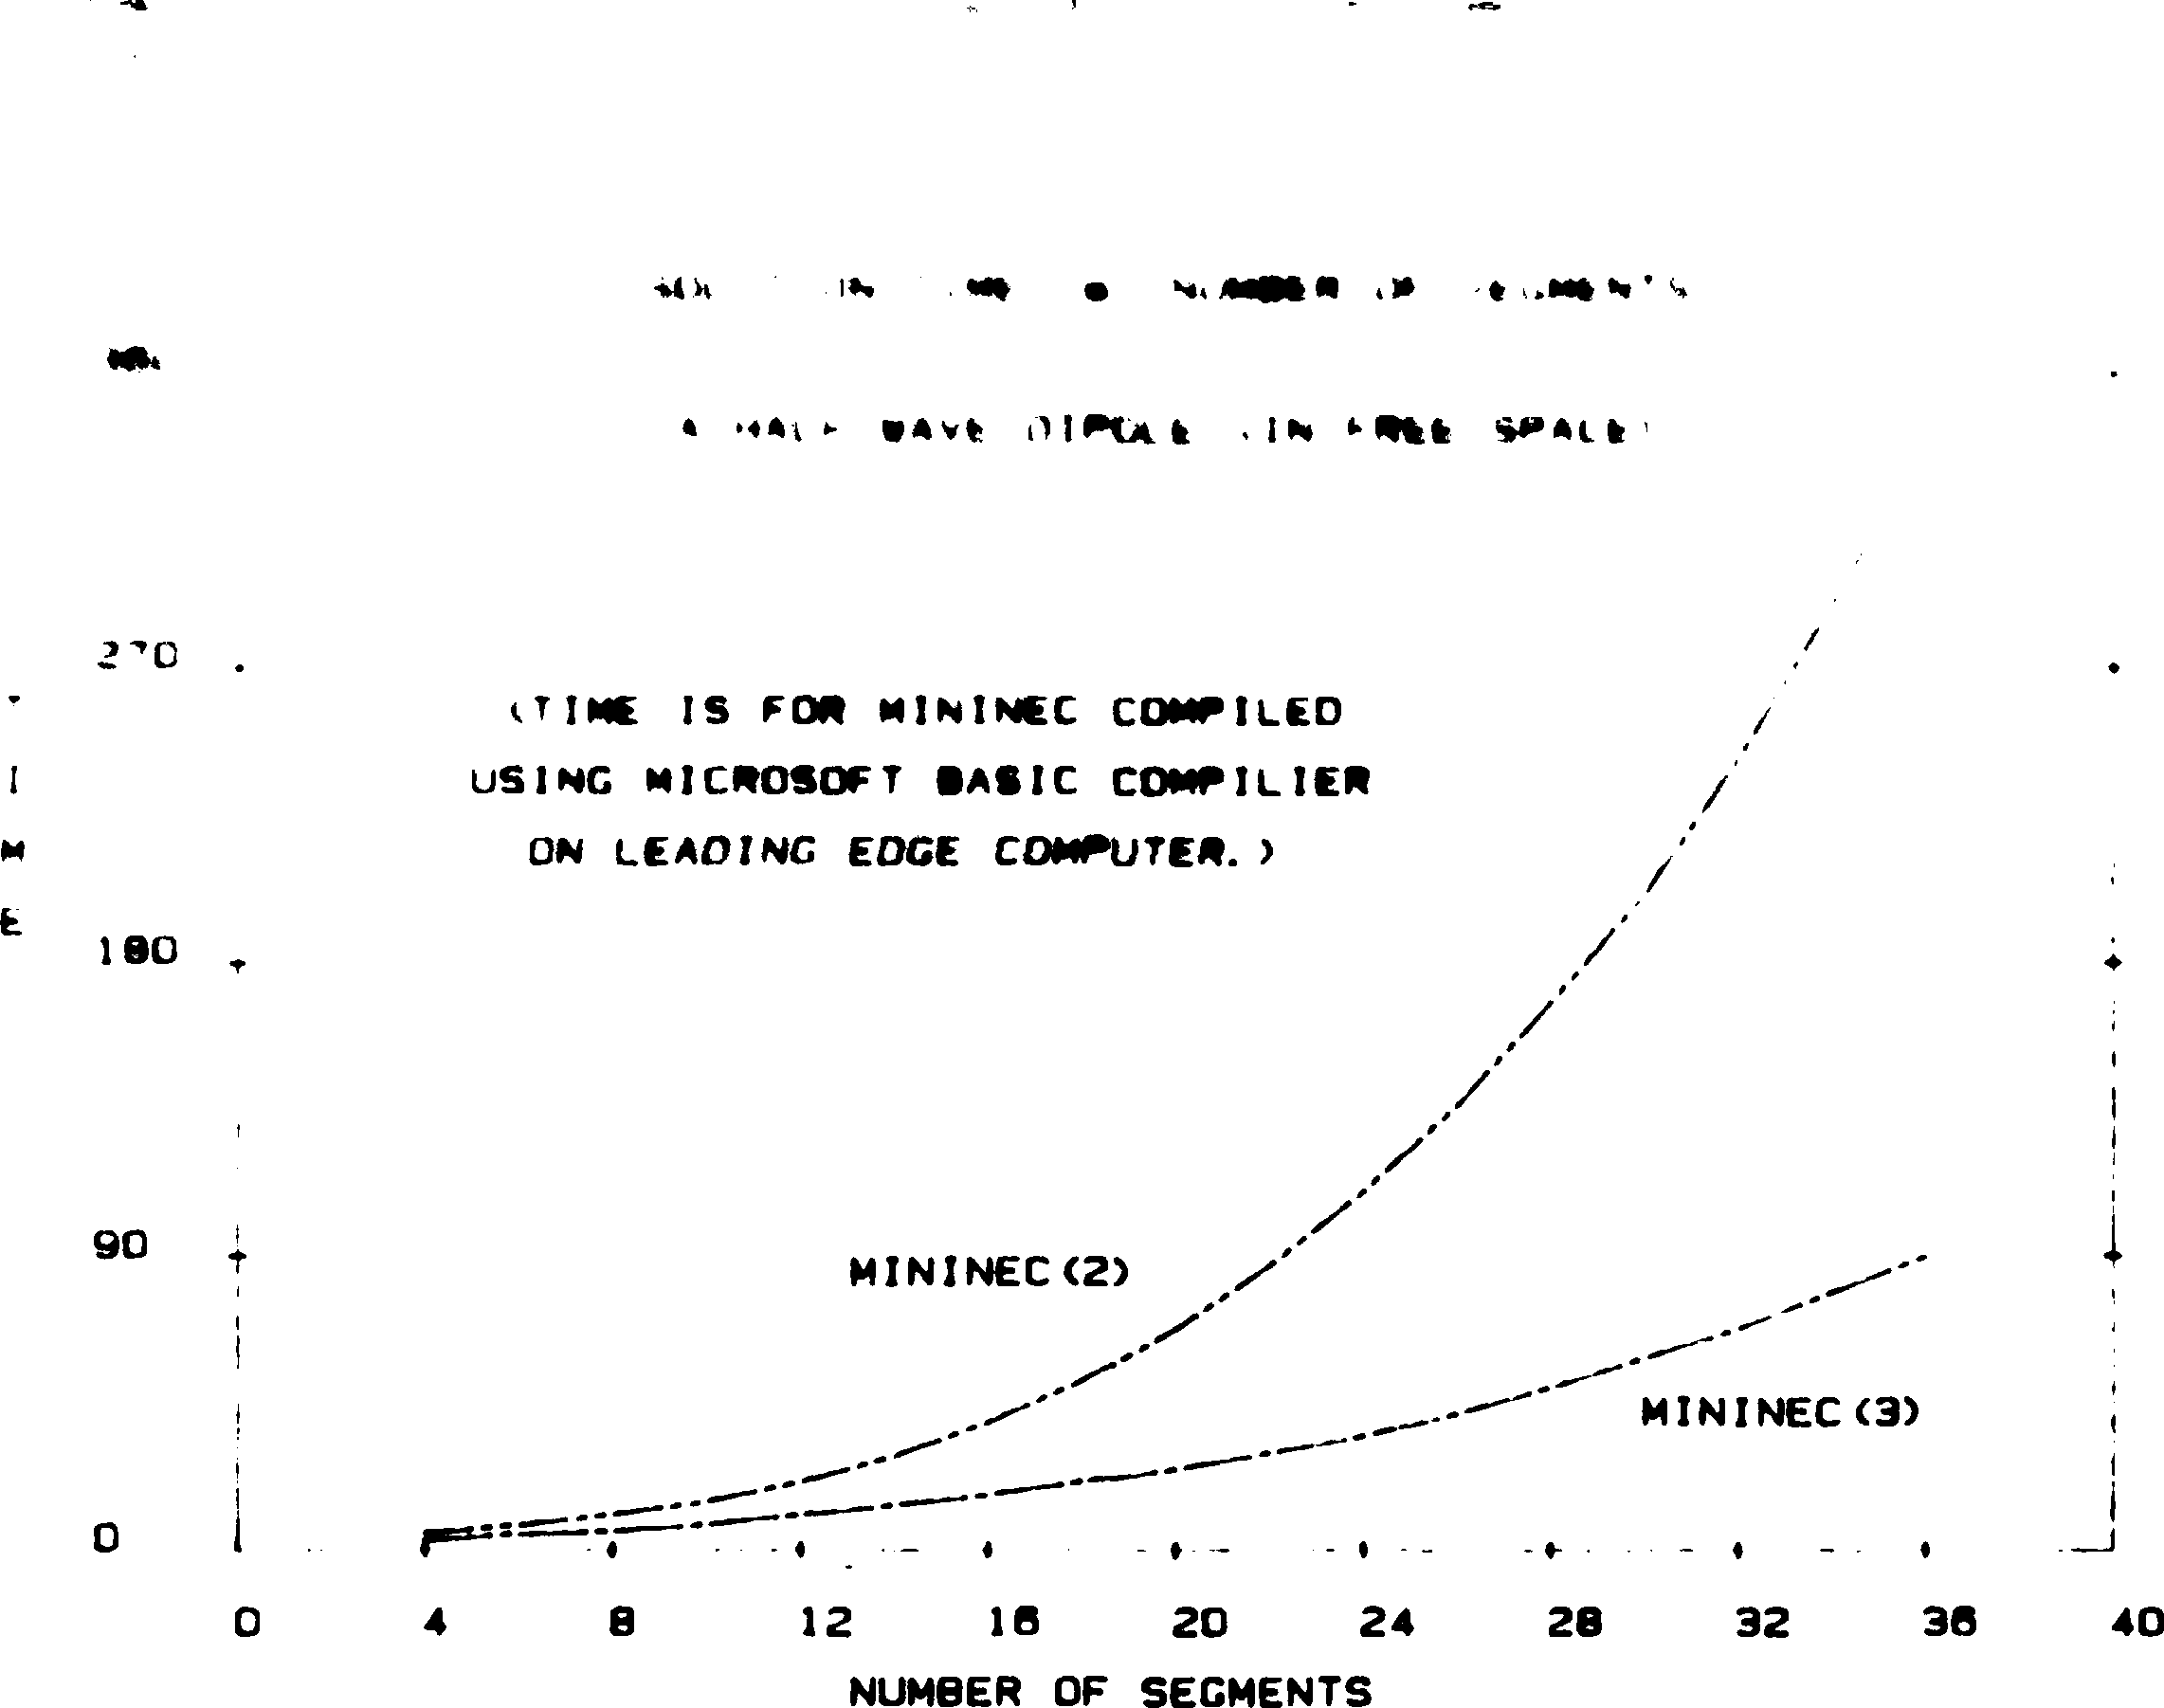
\includegraphics{fig41.eps}}
\caption{A comparison of the run times of MININEC version~2 and~3}
\label{fig41}
\end{sidewaysfigure}

\begin{sidewaysfigure}[htb]
\centerline{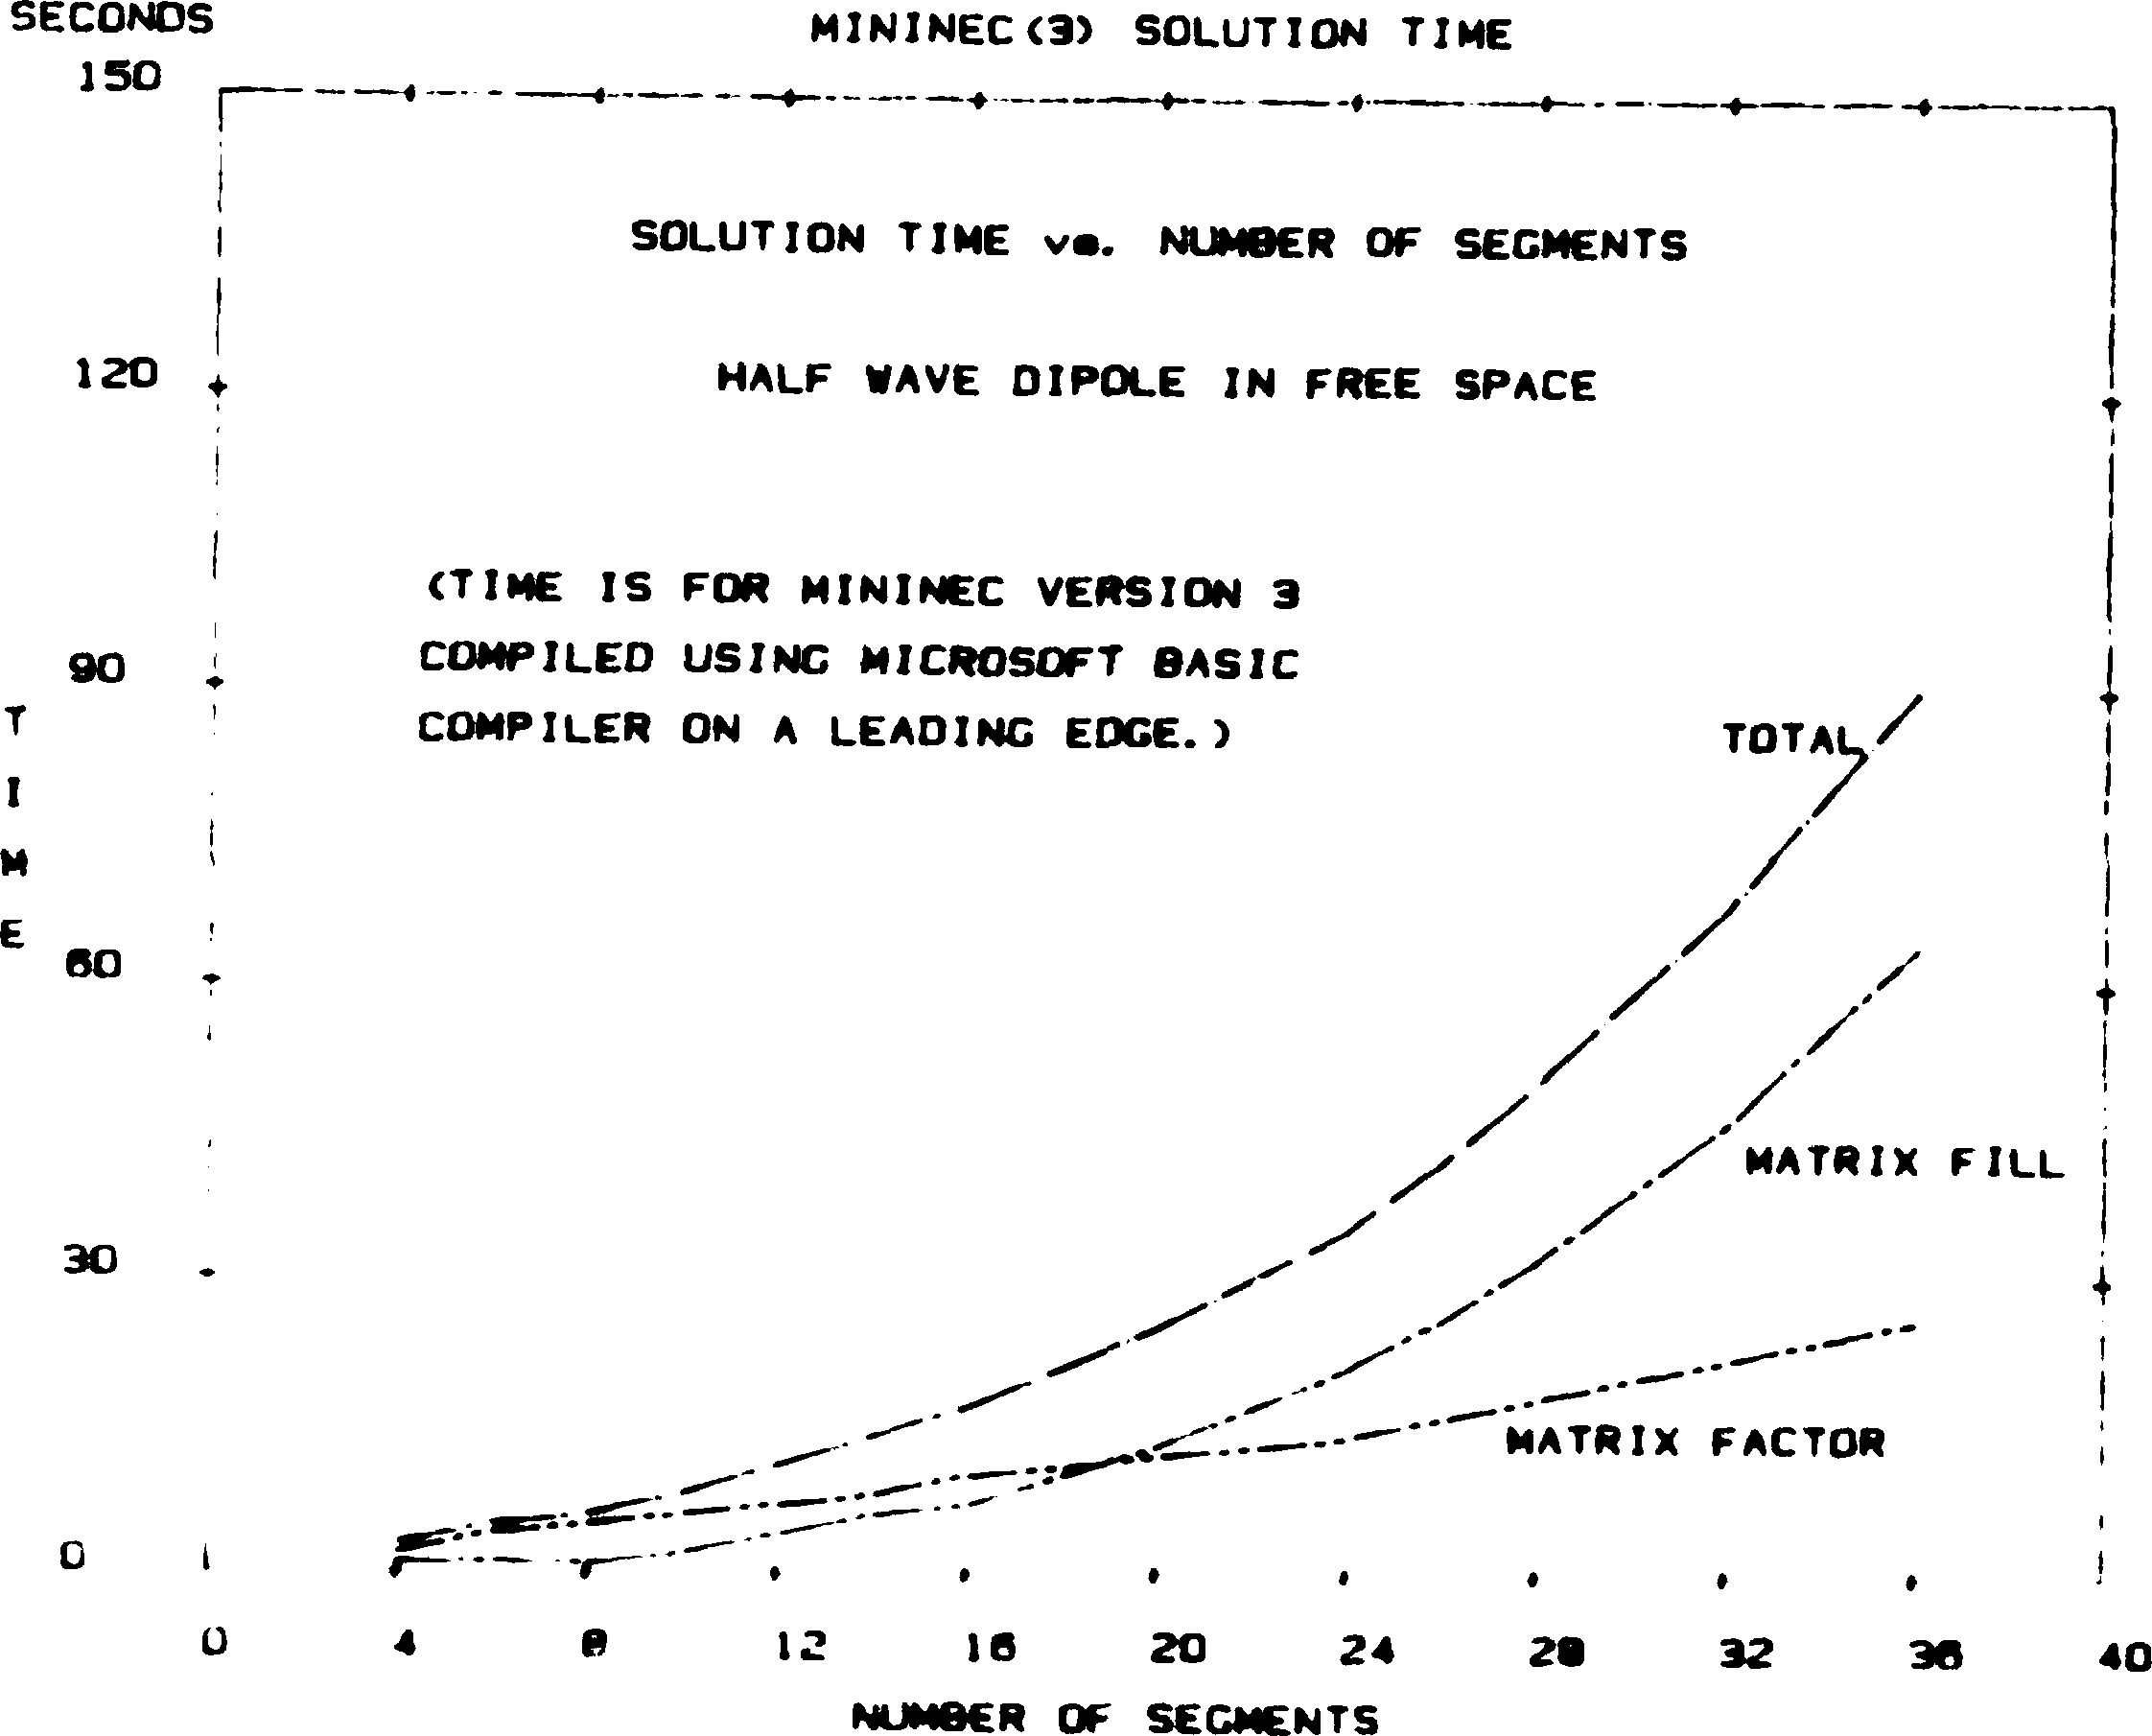
\includegraphics{fig42.eps}}
\caption{Solution time for MININEC(3) to solve a dipole in free space}
\label{fig42}
\end{sidewaysfigure}

\begin{sidewaysfigure}[htb]
\centerline{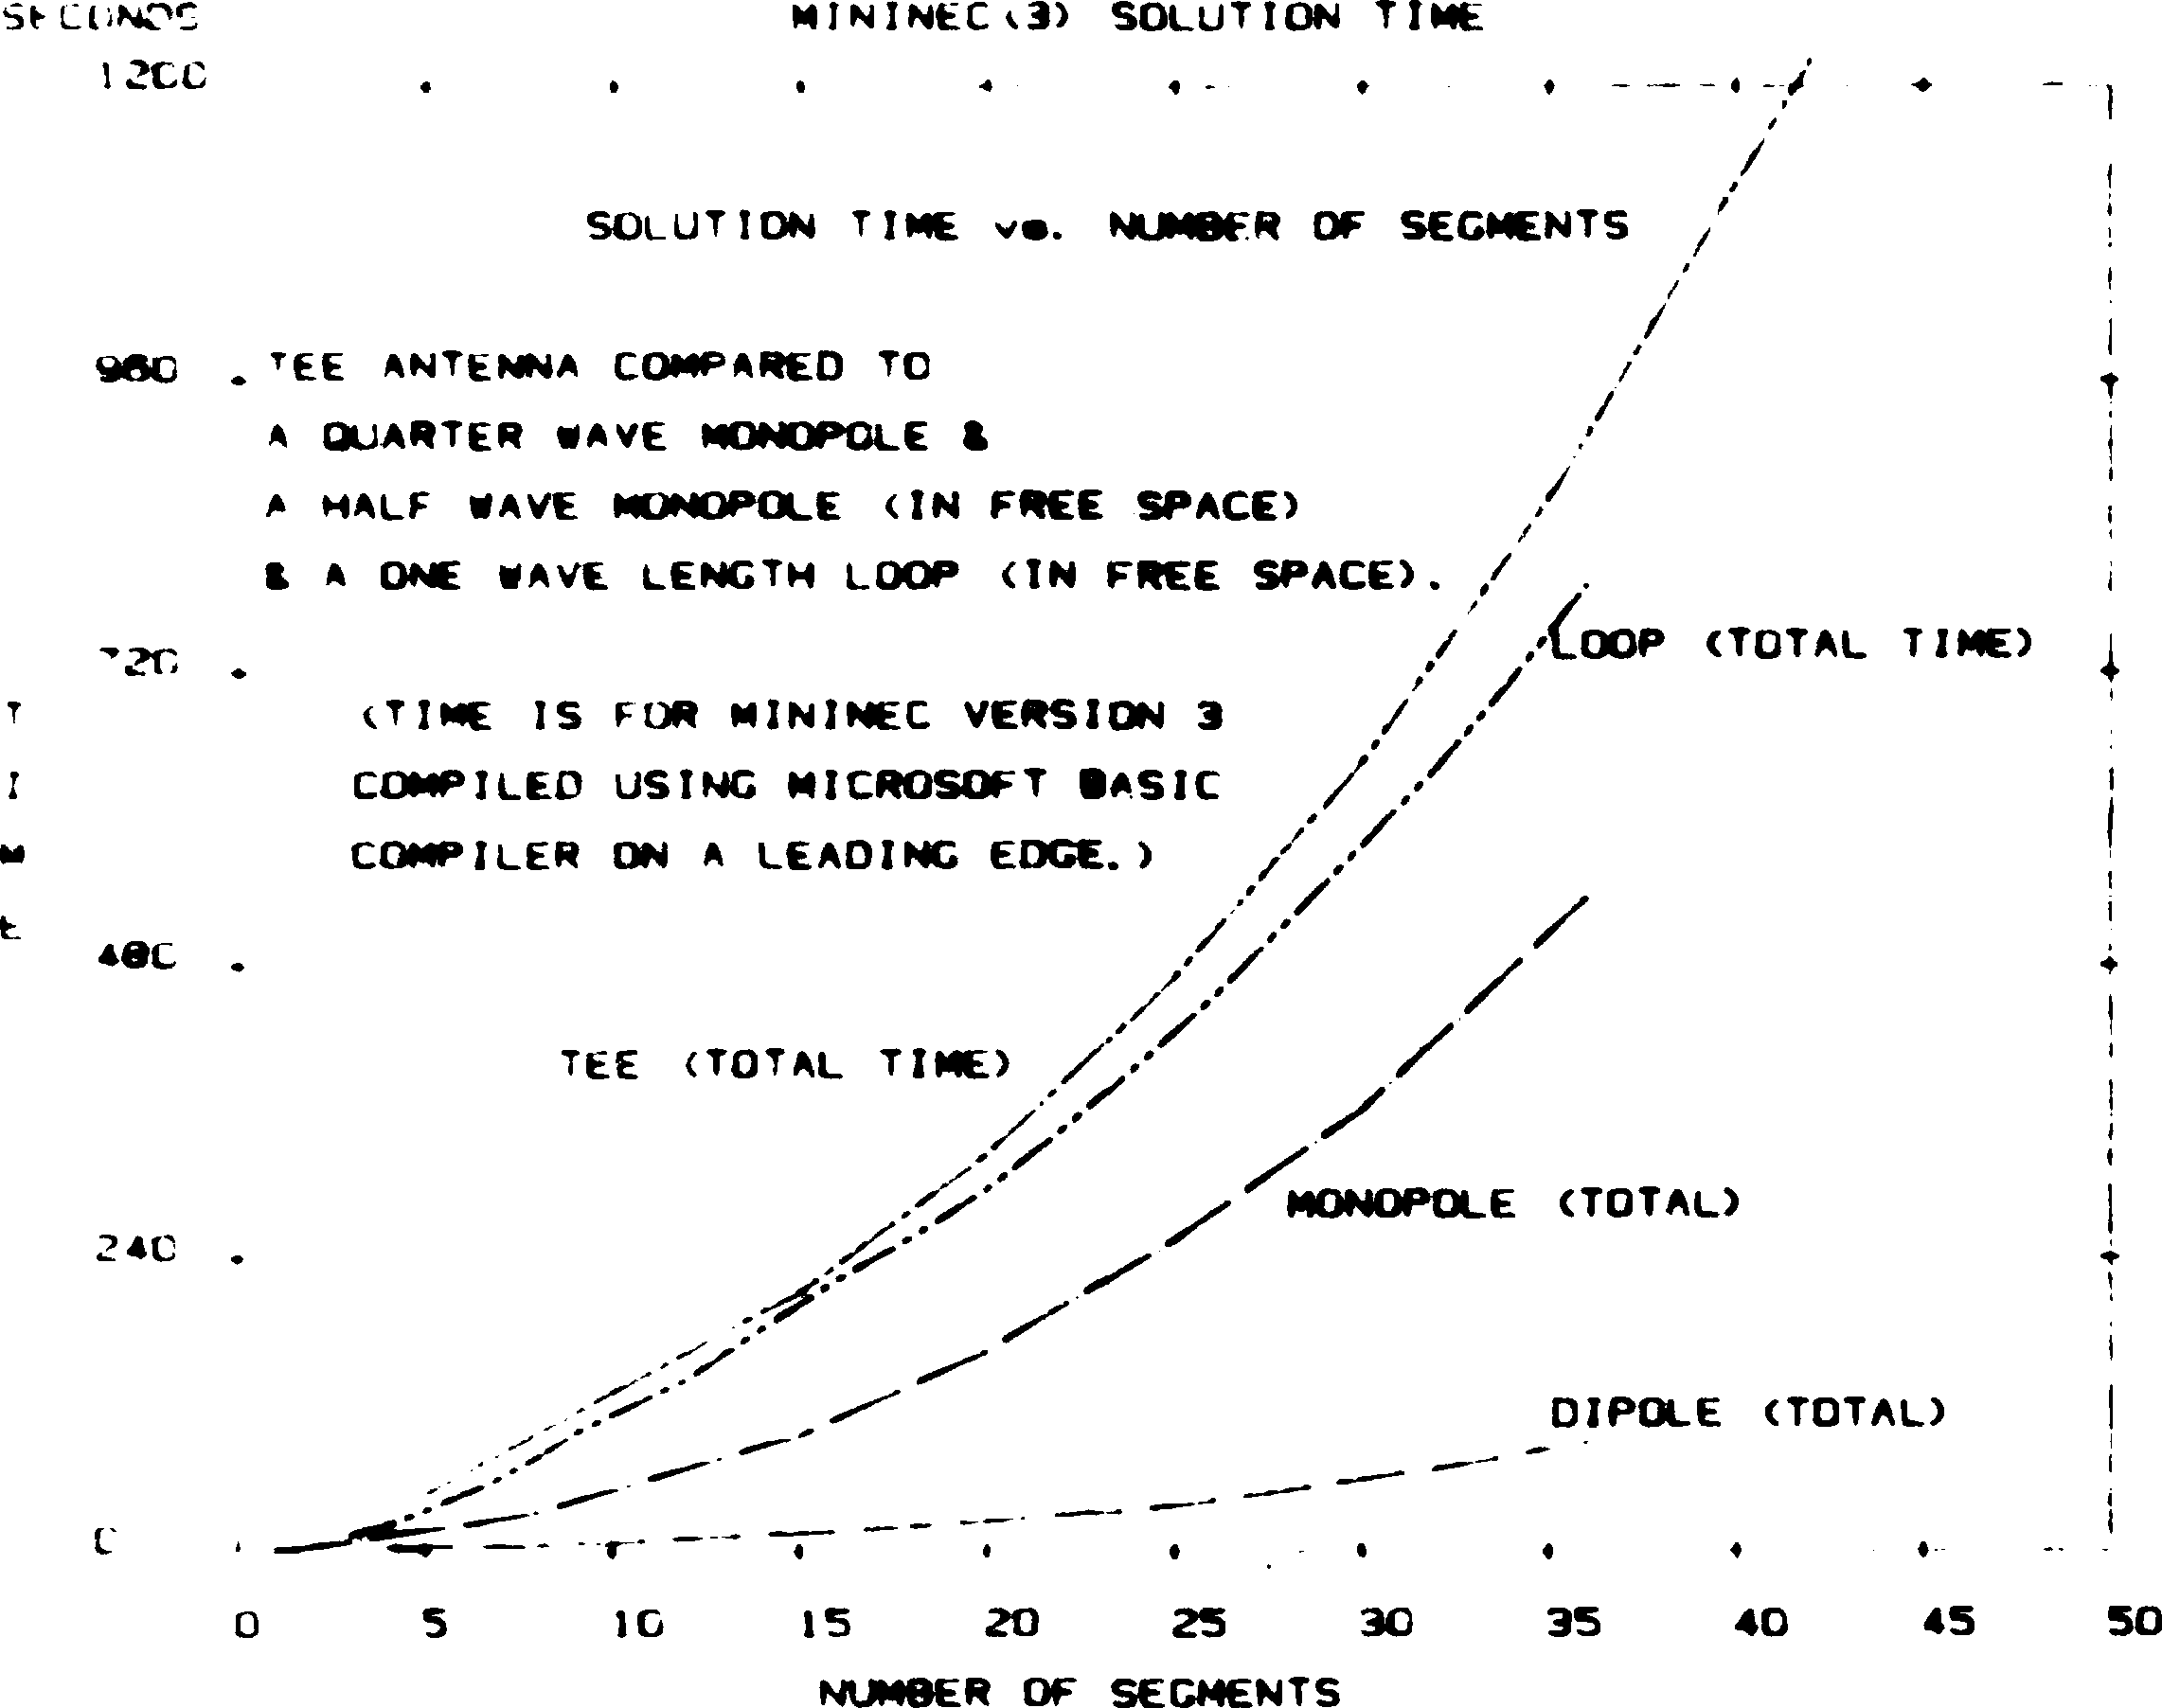
\includegraphics{fig43.eps}}
\caption{Solution time for MININEC(3) to solve a dipole, loop antenna,
monopole and TEE antenna}
\label{fig43}
\end{sidewaysfigure}
\afterpage\clearpage

\subsection{Memory, Disk Storage and Run Time}
Computer memory, disk storage capacity, and solution time are key
limiting factors in the use of all method of moments thin wire antenna
codes because of the need to store and manipulate (solve or invert) a
matrix of complex numbers. These limits are particularly acute when
using a microcomputer. Mega-byte hard disks and compilers can partially
alleviate these limits.

MININEC has been written specifically for the use in the personal
computer environment. Hence the choice of the BASIC language, and the
choice of the simple pulse expansion and testing functions (to keep
overhead down). Every effort has been made to produce a fast compact
computer code. Earlier versions of MININEC were written to minimize
program size (length). The present version, however, has sacrificed size
for improved internal documentation, modularity and increased
capability.

Figure~\ref{fig41} is a comparison of the run times between MININEC
version~2 and MININEC version~3. Both codes were compiled for comparison
using a Microsoft BASIC compiler. Use of a math co-processor will
significantly reduce the run times. The co-processor was not used to
obtain the data in Figure~\ref{fig41}. For comparison, some other
attributes of the codes are as follows:\\

\ \\
\begin{tabular}{lrrrr}
&
\multicolumn{2}{c}{MININEC(2)} &
\multicolumn{2}{c}{MININEC(3)} \\
&
\multicolumn{1}{c}{Interpreter} &
\multicolumn{1}{c}{Compiled}    &
\multicolumn{1}{c}{Interpreter} &
\multicolumn{1}{c}{Compiled}    \\
No. of lines         & 543 & -- & 1607 &  -- \\
\\
Max. no. of wires    &  10 & 75 &   10 &  50 \\
\\
Max. no. of          &  50 & 75 &   30 &  50 \\
\quad segments \\
Disk storage         &  13 & 57 &   44 & 108 \\
\quad (k bytes) \\
\end{tabular}
\ \\

The solution time and size of the executable is a function of the
compiler and the compiler/linker options used.

The significant increase in speed of MININEC(3) is attributable to an
improved solution routine. The matrix fill time, the time to compute all
terms of the matrix, is virtually the same for both versions of MININEC.
For large problems, the fill time is usually longer than the factor
time, the time to solve the matrix. Figure~\ref{fig42} compares the
matrix fill time, factor time and total solution time for MININEC(3) to
solve a dipole in free space. Matrix fill time dominates for problems
above 20 segments.

The solution time not only increases with the number of segments, but
also increases with the number of wire junctions. This effect can be
seen in the data in Figure~\ref{fig43}. Shown is the total solution time
(fill time plus factor time) for a half wave dipole and a loop antenna
in free space. The loop is an extreme case in which the number of wire
junctions equals the number of segments. Also shown in Figure~\ref{fig43}
is the total solution time for a quarter wave monopole and a TEE-antenna
(previously described) over perfect ground. The wire junction in the
TEE-antenna is responsible for the longer solution time compared to the
monopole. The solution time is also longer for antennas over perfect
ground compared to free space. For comparison, the monopole is
equivalent to a dipole in free space with twice the number of segments.
Even so, the dipole solution time is a little shorter than the monopole.

The brute force approach to circumvent memory and solution time limits
is to seek out ever larger, faster computers. The logical extension is
to rewrite MININEC in a more powerful language such as FORTRAN and use a
mainframe computer. But if a mainframe is available, one really should
be using the more powerful NEC program. NEC is written in FORTRAN and is
designed for efficient mainframe use. The concept of MININEC is to use a
personal computer (PC). In time, as PCs become more powerful, then
MININEC, too, will expand in capability. In the meantime, MININEC is
appropriate for application to small problems (less than 100 segments).
Larger problems should be solved with NEC on an appropriate size
computer.

\section{Examples and User Guidance}
This section is intended to be used both as a reference and as a means
for first-time users to become familiar with the input and output (I/O)
options of MININEC. The first-time user should spend a few minutes at
the computer terminal while following along with the simple two-wire
example in section~\ref{sec-getting-started}. A few more minutes at the
terminal (perhaps with a simpler four segment dipole) exploring all of
the MININEC options should be enough to master this skill. However, the
art of actually modeling a wire antenna, i.e., composing the model and
properly interpreting MININEC output, is acquired through considerable
study of antenna theory and properties, study of the data of
section~\ref{sec-validation}, and equally important, accumulating
experience by using MININEC.

\begin{figure}[htb]
\begin{center}
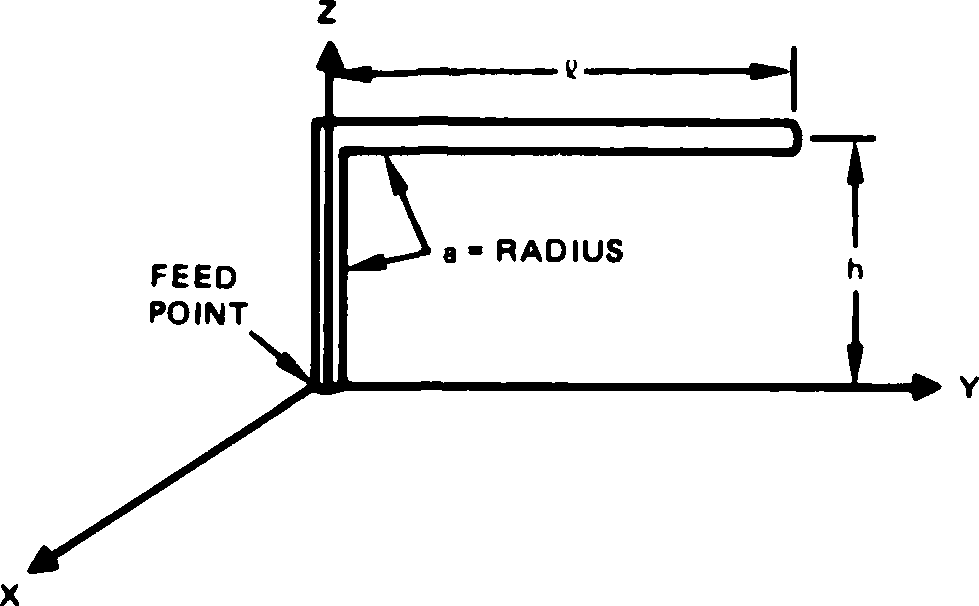
\includegraphics{fig44.eps}
\ \\
\begin{tabular}{ll}
 & $\beta(h+\ell) = ?$     \\
 & $\beta = 2\pi/\lambda$  \\
 & $\beta a = .025$9       \\
\multicolumn{2}{l}{LET $\lambda = 1$, THEN} \\
 & $h   \simeq .191$ m    \\
 & $\ell\simeq .309$ m    \\
 & $a   \simeq .004$ m    \\
 & $Z = 263 - j457\Omega$ \\
\end{tabular}

(Prasad \cite{r18} measured and
corrected for shunt feed
point loading)
\ \\[5mm]
\begin{tabular}{c|l|l|l|c|c}
& \multicolumn{3}{c|}{Coordinates} & & \\
\cline{2-4}
Wire End & X  & Y      & Z     & Wire No. & Wire Radius \\
\hline
1        & 0. & 0.     & 0.    & \multirow{2}{*}{1} & \multirow{2}{*}{.004} \\
\cline{1-4}
2        & 0. & 0.     & 0.191 &                    & \\
\hline
1        & 0. & 0.     & 0.191 & \multirow{2}{*}{2} & \multirow{2}{*}{.004} \\
\cline{1-4}
2        & 0. & 0.309  & 0.191 &                    & \\
\end{tabular}
\ \\[5mm]
\begin{tabular}{c|c|c}
\multicolumn{3}{c}{Segmentation}                \\
\multicolumn{3}{c}{Suggested Convergence Test}  \\
Wire 1 & Wire 2 & Total \\
\hline
\ 4 & \ 6 & 10 \\
\ 6 & \ 9 & 15 \\
\ 8 & 12  & 20 \\
10  & 15  & 25 \\
12  & 18  & 30 \\
\end{tabular}
\end{center}
\caption{Inverted L-antenna data for the example in
Section~\ref{sec-getting-started}}
\label{fig44}
\end{figure}
\afterpage\clearpage

\subsection{Getting Started}
\label{sec-getting-started}
First, gather up all known information on the antenna to be modeled,
including measurements or reliable analytical data, if available. It is
helpful to make a sketch of the antenna using any convenient cartesian
coordinate system. For this example, please consider the interted
L-antenna in Figure~\ref{fig41}. You will need to know the X, Y, Z
location for each wire end of each wire relative to the origin of your
choice. And you will need to know the radius of each wire. All
dimensions must be in meters. This information for the example can be
found in Figure~\ref{fig44}.

You will need to decide how many segments to use on each wire. This may
be done initially by calculating the length of each wire in wave lengths
at the desired frequency. Then refer to Figures~\ref{fig6}
through~\ref{fig11} as appropriate for the initial choice. This will not
guarantee that the MININEC solution will be well converged, but it
provides a good place to start. A convergence test is always a good
idea. A possible segmentations scheme for the inverted L-antenna is
suggested in Figure~\ref{fig44}. Alternatively, using your prior
experience on a similar antenna, you may be able to come closer to the
converged solution the first time. For example, the inverted L-antenna
is one wire short of being a TEE-antenna similar to the ones in
section~\ref{sec-monopoles} (see Figures~\ref{fig28} through~\ref{fig31}).
For the purpose of this discussion, however, we will use a minimal
number of segments in order to keep the solution time reasonably short.

MININEC is designed for demand mode execution. Therefore, all you need
to do is answer the questions when prompted or provide the required data
appropriately. In general, you must define the antenna geometry and
define the environment. MININEC can then solve for the currents. Once
MININEC has the solution, you may then request near and far fields
(patterns).

Now run MININEC. The first question you must answer is:

\begin{Verbatim}
OUTPUT TO CONSOLE, PRINTER, OR DISK (C/P/D)?
\end{Verbatim}

If you enter \verb+C+ for console, all data will be displayed on the
monitor. If you answer \verb+P+ for printer, the questions or prompts
will still be displayed on the monitor, but all other data will be
printed. If you answer \verb+D+ for disk, you will then be prompted to
supply the name of a disk file for storage of all MININEC output:

\begin{Verbatim}
OUTPUT TO CONSOLE, PRINTER, OR DISK (C/P/D)?  D
FILENAMES (NAME.OUT)?
\end{Verbatim}

As with the printer, all questions and prompts appear on the monitor,
but the results go to the file you specify.

Next you must supply the frequency in MHz. Enter the desired frequency
or simply enter return to select the default value of 299.8 MHz (or a
wave length of one meter).

\begin{Verbatim}
FREQUENCY (MHz)?
    WAVE LENGTH = 1 METER
\end{Verbatim}

For the next question, you must select free space or a ground plane by
entering 1 or -1, respectively.

\begin{Verbatim}
ENVIRONMENT (+1 FOR FREE SPACE, -1 FOR GROUND PLANE)?
\end{Verbatim}

If you select -1 for ground, you are then prompted for the number of
media, which must be an integer from zero to 5.

\begin{Verbatim}
ENVIRONMENT (+1 FOR FREE SPACE, -1 FOR GROUND PLANE)?  -1
 NUMBER OF MEDIA (0 FOR PERFECTLY CONDUCTING GROUND)?
\end{Verbatim}

A zero selects a perfectly conducting ground plane. See
Section~\ref{sec-change-env} for further details. Suffice to say at this
point that selection of 1 to 5 media does not effect the current
distribution or the antenna impedance, but only effects far field
calculations. Please select a zero to continue along with this
narrative.

Next, you must specify the number of wires\footnote{Note to NEC users:\\
The MININEC post processor program is used to convert a NEC input data
set into a MININEC antenna geometry description. These data are
automatically stored in the \texttt{MININEC.INP} file. At this point, in
the \texttt{MININEC.INP} file is not empty, MININEC will use that data for
the geometry description and you will skip the normal geometry input.
See Appendix~\ref{sec-appendix-a} for further information.}. If you
specify more than the number allowed, a warning message appears and the
question is repeated.

\begin{Verbatim}
NO. OF WIRES?  100
NUMBER OF WIRES EXCEEDS DIMENSION. . .
NO. OF WIRES?
\end{Verbatim}

\noindent A zero will place you at the main menu.

\begin{Verbatim}
NO. OF WIRES?  0

********************    MININEC MENU    ********************
   G - CHANGE GEOMETRY     C - COMPUTE/DISPLAY CURRENTS
   E - CHANGE ENVIRONMENT  P - COMPUTE FAR-FIELD PATTERNS
   X - CHANGE EXCITATION   N - COMPUTE NEAR-FIELDS
   L - CHANGE LOADS/NET    Q - QUIT
   F - CHANGE FREQUENCY
************************************************************
   COMMAND?
\end{Verbatim}

\noindent To recover from this point, select \verb+G+ for change
geometry and answer the questions on environment again.

\begin{Verbatim}
NO. OF WIRES?  0

********************    MININEC MENU    ********************
   G - CHANGE GEOMETRY     C - COMPUTE/DISPLAY CURRENTS
   E - CHANGE ENVIRONMENT  P - COMPUTE FAR-FIELD PATTERNS
   X - CHANGE EXCITATION   N - COMPUTE NEAR-FIELDS
   L - CHANGE LOADS/NET    Q - QUIT
   F - CHANGE FREQUENCY
************************************************************
   COMMAND?  G

ENVIRONMENT (+1 FOR FREE SPACE, -1 FOR GROUND PLANE)?  -1
 NUMBER OF MEDIA (0 FOR PERFECTLY CONDUCTING GROUND)?  0

NO. OF WIRES?
\end{Verbatim}

Let's assume two wires. The next prompt is for the number of segments on
wire~1.

\begin{Verbatim}
WIRE NO. 1
    NO. OF SEGMENTS?
\end{Verbatim}

You will be prompted for each wire in turn. If you answer zero, you will
return to the question for the number of wires. This is a convenient
escape mechanism, sometimes useful when you change your mind.

\begin{Verbatim}
WIRE NO. 1
    NO. OF SEGMENTS?  0

NO. OF WIRES?  2

WIRE NO. 1
    NO. OF SEGMENTS?
\end{Verbatim}

If at any time you specify too many segments on any one wire, or the
total number of segments on all wires specified becomes larger than the
maximum allowed by the program array dimensions, an error message will
be displayed, and you will return to the question for the number of
wires. In this case, to keep this session short, let's choose 4~segments
for wire~1.

Next, enter the X, Y, Z coordinates, in meters, for end one of the first
wire. Then enter the X, Y, Z coordinates for end two; then enter the
radius, as prompted.

\begin{Verbatim}
NO. OF SEGMENTS?  4
END ONE COORDINATES (X,Y,Z)?  0,0,0
END TWO COORDINATES (X,Y,Z)?  0,0,.191
                     RADIUS?  .004
            COORDINATES                                 END         NO. OF
   X             Y             Z          RADIUS     CONNECTION     SEGMENTS
0             0              0                          -1
0             0             .091          .004           0             4
   CHANGE WIRE NO.  1  (Y/N)?
\end{Verbatim}

After entry of the radius, MININEC responds immediately with a table as
shown above. The table gives the coordinates of the wire ends, the
radius and the end connection information, so you may verify that you
have entered the data correctly. If not, you have the opportunity to
start again with this wire. Otherwise, you may continue to the next
wire. The end connection information is useful to verify that a
connection has been made. In this case, the minus one indicates that end
one in connected to ground. A connection to ground is indicated by a
negative integer, whose absolute value is the same as the wire number.
The zero indicates that end two of this wire is not yet connected to any
other wire.

Now continue on to the next wire and give the appropriate data:

\begin{Verbatim}
CHANGE WIRE NO.  1  (Y/N)?  N

WIRE NO. 2
   NO. OF SEGMENTS?  6
   END ONE COORDINATES (X,Y,Z)?  0,0,.191
   END TWO COORDINATES (X,Y,Z)?  0,.309,.091
                           RADIUS?  .004
            COORDINATES                                 END         NO. OF
   X             Y             Z          RADIUS     CONNECTION     SEGMENTS
0             0              .191                         1
0             .309           .191          .004           0            6
CHANGE WIRE NO.  2  (Y/N)?
\end{Verbatim}

The connection data indicates that end one of wire two is connected to
the top of wire one, i.e., end two of wire one. The absolute value of
the end connection integer is the wire number to which wire two is
connected. A plus sign indicates an end one connected to an end two (as
in this case), or an end two connected to an end one. A negative sign
indicates and end one connected to an end one, or an end two connected
to an end two. And, of course, a zero means no connection.

By the way, if you happen to give either wire end a negative
Z-coordinate when a ground plane is specified, you will get an error
message and will have to reconsider your entry. Likewise, MININEC will
not let you get away with a zero radius, or a zero wire length.

If you are now satisfied with the wire two data entry, we may proceed.
MININEC will produce a table of the coordinates for the location of each
current pulse on each wire. Note that the radius and connection data are
also given so that you may verify your data entry.

\begin{Verbatim}
CHANGE WIRE NO.  2  (Y/N)?  N

                  **** ANTENNA GEOMETRY ****

WIRE NO.  1  COORDINATES                                CONNECTION PULSE
X             Y             Z             RADIUS        END1 END2  NO.
 0             0             0             .004          -1    1    1
 0             0             .04775        .004           1    1    2
 0             0             .0955         .004           1    1    3
 0             0             .14325        .004           1    0    4

WIRE NO.  2  COORDINATES                                CONNECTION   PULSE
X             Y             Z             RADIUS        END 1 END 2  NO.
 0             0             .191          .004           1     2      5
 0             .0515         .191          .004           2     2      6
 0             .103          .191          .004           2     2      7
 0             .1545         .191          .004           2     2      8
 0             .206          .191          .004           2     2      9
 0             .2575         .191          .004           2     0     10

CHANGE GEOMETRY (Y/N)?
\end{Verbatim}

This table is essential to proper location of the feed point (or source
excitation point) and location of loads.

You now have one last chance to change the geometry before proceeding.

\begin{Verbatim}
CHANGE GEOMETRY (Y/N)?  N

NO. OF SOURCES?
\end{Verbatim}

You must now decide how many feed points to use, where they are located,
and what voltages are applied. You will be prompted for this data for
each source, in turn. In this case, let's keep it simple.

\begin{Verbatim}
NO. OF SOURCES?  1

SOURCES NO. 1:
PULSE NO., VOLTAGE MAGNITUDE, PHASE (DEGREES)?  1,1,0
\end{Verbatim}

Sources are always co-located with current pulse functions. Hence, you
may have to refer to the above table of antenna geometry to select an
appropriate pulse to apply the source. In this example, the source is at
the ground plane, i.e., pulse number one, located on wire one. I have
chosen one volt at zero degree phase angle for this example.

The next set of questions provide the opportunity to add impedance
loading to the antenna. To keep things simple, let's avoid loading and
continue on. Please refer to section~\ref{sec-loads} for more detailed
information on loading options.

\begin{Verbatim}
NUMBER OF LOADS?  0

********************    MININEC MENU    ********************
   G - CHANGE GEOMETRY     C - COMPUTE/DISPLAY CURRENTS
   E - CHANGE ENVIRONMENT  P - COMPUTE FAR-FIELD PATTERNS
   X - CHANGE EXCITATION   N - COMPUTE NEAR-FIELDS
   L - CHANGE LOADS/NET    Q - QUIT
   F - CHANGE FREQUENCY
************************************************************
   COMMAND?
\end{Verbatim}

You are now faced with the main menu again. By selection of an
appropriate command letter, you may change the geometry (\verb+G+),
change the environment (\verb+E+), change the source or excitation
(\verb+X+), change the loads and networks (\verb+L+), and change the
frequency. When satisfied with the antenna geometry and environment, you
are ready to determine the antenna properties. The preferred choice at
this point is \verb+C+, compute and display the currents. If you select
\verb+P+ for patterns or \verb+N+ for near fields, MININEC will check to
see if the currents have been calculated; if not, MININEC will compute
the currents before you can proceed. So let's select \verb+C+.

\begin{Verbatim}
   COMMAND?  C

   BEGIN MATRIX FILL
   MATRIX FILL 10% COMPLETE - APPROX TIME REMAINING 1:48
\end{Verbatim}

MININEC responds almost immediately with an estimate of the time in
minutes and seconds required to complete filling the impedance matrix.
At intervals, the estimate will be updated and the total time will be
given when this step is completed. Similarly, MININEC will estimate the
time to solve the matrix for the currents and in turn display the total
times.

\begin{Verbatim}
   BEGIN MATRIX FILL
   MATRIX FILL 100% COMPLETE - APPROX TIME REMAINING 0:00
   FILL MATRIX:  1:27

   FACTOR MATRIX 100% COMPLETE - APPROX TIME REMAINING 0:00
   FACTOR MATRIX:  0:04
\end{Verbatim}

When the solution is complete, MININEC computes and displays the
impedance and power input for each source in turn. If there is more than
one source, the sum total power input will also be displayed. The
solution is also displayed in terms of the current distribution, wire by
wire.

\begin{Verbatim}
********************    SOURCE DATA     ********************
PULSE  1      VOLTAGE = ( 1 , 0 J)
              CURRENT = ( 9.852278E-04 , 1.479977E-03 J)
              IMPEDANCE = ( 311.6818 , -468.1982 J)
              POWER =  4.926139E-04  WATTS

********************    CURRENT DATA    ********************


WIRE NO.  1:
PULSE        REAL          IMAGINARY     MAGNITUDE     PHASE
NO.          (AMPS)        (AMPS)        (AMPS)        (DEGREES)
 1           9.852278E-04   1.479977E-03  1.777922E-03  56.3481
 2           .000962       -7.880544E-04  1.243573E-03 -39.32376
 3           8.940962E-04  -2.186383E-03  2.362143E-03 -67.75855
 4           7.867739E-04  -3.248648E-03  3.342563E-03 -76.38595
J            6.45715E-04   -3.943692E-03  3.996205E-03 -80.70126

WIRE NO.  2:
PULSE        REAL          IMAGINARY     MAGNITUDE     PHASE
NO.          (AMPS)        (AMPS)        (AMPS)        (DEGREES)
J            6.45715E-04   -3.943692E-03  3.996205E-03 -80.70126
 6           5.160325E-04  -4.466384E-03  4.496095E-03 -83.40944
 7           3.756805E-04  -4.519859E-03  4.535446E-03 -85.24862
 8           2.408057E-04  -4.093055E-03  4.100132E-03 -86.633
 9           1.252218E-04  -3.201494E-03  3.203942E-03 -87.76009
 10          4.12146E-05   -1.891714E-03  1.892163E-03 -88.75189
E            0              0             0             0

SAVE CURRENTS TO A FILE (Y/N)?
\end{Verbatim}

Notice that the current is zero at the free end of wire two. And since
there is no pulse number, an \verb+E+ is displayed to help identify a
free end. Kirchoff's current law has been used to solve for the currents
on each respective wire at the junction. And a \verb+J+ is substituted
for the pulse number, indicating a wire junction or connection point.

Notice that the real part of the impedance, the resistance, is within
19\% of the measured value given by Prasad \cite{r18}, (see
the data in Figure~\ref{fig44}) and the reactance is within 2.4\%. When
I tried the convergence test suggested by the scheme in Figure~\ref{fig44},
MININEC was pretty well converged at 30 segments to an impedance of
167 + j395 ohms. Prasad used an approximate method to correct her
measured data for the loading effects of the coaxial termination at the
feed point. I suspect the method may not be sufficiently accurate in
this case.

You must now decide whether to save the currents to a disk file. If you
answer \verb+Y+, you will be prompted for a disk file name and the
currents will be saved. If not, you will return to the main menu.

\clearpage
\begin{Verbatim}
SAVE CURRENTS TO A FILE (Y/N) ? N

********************    MININEC MENU    ********************
   G - CHANGE GEOMETRY     C - COMPUTE/DISPLAY CURRENTS
   E - CHANGE ENVIRONMENT  P - COMPUTE FAR-FIELD PATTERNS
   X - CHANGE EXCITATION   N - COMPUTE NEAR-FIELDS
   L - CHANGE LOADS/NET    Q - QUIT
   F - CHANGE FREQUENCY
************************************************************
   COMMAND?
\end{Verbatim}

If you decide that you want to look at the impedance or currents again,
you simply chose \verb+C+. There is no wait this time because MININEC
does not re-compute and solve the matrix. You will get an immediate
display of the impedance and currents.

You may now elect to calculate patterns or near fields. Please refer to
the appropriate sections for details on these operations.

Good luck!

\subsection{Change Geometry}
The \verb+G+ option on the MININEC menu provides the means to change the
antenna configuration without changing the frequency. The entry point is
the question to choose the environment, free space or ground. Please see
section~\ref{sec-change-env} for details. After choosing the environment, you
will begin defining the wire configuration, i.e., specify the number of
wires and the location, radius and segmentation for each wire. Please
see section~\ref{sec-getting-started} for an example.

\subsection{Change Environment}
\label{sec-change-env}
The \verb+E+ option on the MININEC menu provides the means to change the
antenna environment, without changing the frequency, feed point, loading
or geometry. Note that changing from free space to a ground plane does
not change the connection data or location of wires already specified.
Hence, erroneous and strange results may occur if the geometry is not
also changed appropriately.

Selecting free space will return you to the main menu.

If you choose a ground plane, you may specify 0 for perfectly conducting
ground or you may select up to 5 changes in surface impedance (up to 5
media). Changing the surface impedance does not alter the current
distribution on antennas over ground. MININEC uses the surface impedance
to correct far field pattern only. If you select 1 surface impedance,
you will be prompted for the relative dielectric constant and the
conductivity, in mhos per meter. The far field subroutine will use this
information in a Fresnel reflection coefficient correction to the
radiation fields.

For two or more impedance surfaces, you must choose between a linear or
circular boundary between surfaces. The linear boundary is parallel to
the Y-axis. The circular boundary is centered at the origin. The first
surface (and the perfectly conducting ground plane) is always at the
level of the X-Y plane (Z=0). For each surface in turn, you must specify
the height of the surface (or media) relative to the first surface. A
negative value is a step down; a positive value is a step up. A zero
value means a flat ground. Note that there is no diffraction coefficient
correction in MININEC for a cliff edge. There is also no correction for
blockage due to a large step up, i.e., the antenna cannot be in a well.
For each media in turn, you must supply the distance in meters from the
origin to the media boundary.

When you choose a circular boundary with two or more media, you will be
prompted for the number of radial wires in the ground screen. This
approximation is really accurate for dense ground screens only. One
hundred or more should be used for best results. Zero, of course, is
also a valid choice. You must also supply the wire radius of the wires
in the ground screen. The length of the wires in the ground screen is
the same as the distance to the interface between media one and two.

\subsection{Change Excitation}
The \verb+X+ option in the MININEC menu provides the means to change the
antenna feed excitation (i.e., number of feeds, feed location and
magnitude and phase) without changing the geometry, environment,
frequency or loading. Changing only the excitation does not require
re-filling or re-factoring of the matrix. Hence, after solving for the
currents for the initial excitation, you can rapidly try out all
possible source locations or try multiple source excitation. Source
locations must coincide with the locations of the current pulse
functions. You cannot put source excitations on non-existent pulses. At
least one source must be given. MININEC will not allow more sources than
the maximum set by the dimension statement (see the first 30~lines of
MININEC to determine this limit).

There is but one source model in MININEC. The model imposes a constant
field over a pulse width, with amplitude and location, coincident with a
current pulse, chosen by the user. In spite of the simplicity, this
source model is a good approximation for most transmit cases. What do
you do then to evaluate the performance of a receive only antenna? One
way to evaluate the receive properties of an antenna is to place a
transmitting dipole at a great distance (i.e., in the far field of the
receive antenna). The field incident on the receive antenna is a good
approximation to a plane wave.

\subsection{Change Loads}
\label{sec-loads}
The \verb+L+ option on the MININEC menu provides the means to alter or
add lumped parameter loads to an antenna. Changing the load requires
re-filling and re-factoring of the matrix. Each load location must
coincide with a current pulse function. MININEC will not allow more
loads than the maximum for which it is dimensioned (see the first
30~lines of MININEC to determine this limit). There are two kinds of
loads; impedance loading and S-parameter loading. You may select the
loading type when prompted after specifying the number of loads.

The simplest load type is impedance loading. You must supply the pulse
location, resistance and reactance for each load, in turn. The reactance
value you specify will not change when you change the frequency. If you
desire the load impedance to change appropriately with frequency, you
must change the impedance load every time you change frequency.
Alternatively, you may specify your load in terms of an equivalent
S-parameter function.

One convenient method of circuit analysis makes use of the concept of a
complex frequency, or S-paramter. Generally, $S$ is defined as
$S=G+\jj\omega$ where $G$ is the neper frequency and $\omega$ is the
angular frequency \cite{r24}. For steady state, sinusoidal
time varying signals, $G=0$.

The impedance of an RLC circuit can always be expressed as a function of
$S$. With a little bit of algebra, the impedance can be represented as a
ratio of polynomials in $S$. The S-parameter impedance function is a
polynomial in $S$ with the form:

\[ Z(S) = \frac{A_0S^0+A_1S^1+A_2S^2+\ldots A_nS^n}
               {B_0S^0+B_1S^1+B_2S^2+\ldots B_mS^m}
\]

where the coefficients $A_i$ and $B_i$ are functions of R, L and C. For
example a series RC circuit has an impedance of

\[ Z = R + \frac{1}{j\omega C} = R + \frac{1}{SC} = \frac{RC+1}{CS}
\]

hence
\[A_0 = RC + 1 \]

\[A_1 = 0 \mbox{ for }i > 0 \]

and

\[B_0 = 0\]

\[B_1 = C\]

\[B_i = 0 \mbox{ for }i>1\]

When you select the S-parameter load option, you will be prompted for
the pulse number (at which to locate each load) and the order of the
S-parameter impedance function. The order is the highest exponent of $S$
occurring in either the numerator or denominator. For the example cited
above, the order is one. After supplying these two numbers, you will be
prompted for the magnitude of the coefficients of $S$ in order, starting
with the order zero and up to the order you have specified. The
coefficients are given in pairs, i.e., numerator and denominator for
each order.

The advantage of the S-parameter load is that the impedance changes
appropriately with frequency. Each time you change frequency, you need
not re-specify the load. Almost any series-parallel combination of RLC
elements can be expressed in terms of a polynomial in $S$, with a little
bit of algebraic effort.

\subsection{Change Frequency}
The \verb+F+ option on the MININEC menu provides a way to alter the
frequency. You will be prompted for the frequency in MHz. MININEC will
compute and display the wave length and return to the menu. Changing the
frequency will require re-filling and re-factoring of the impedance
matrix. The current geometry will be used.

\subsection{Compute/Display Currents}
The \verb+C+ option on the MININEC menu triggers filling and factoring
of the matrix for the antenna configuration most recently specified. If
a solution has already been computed, and no changes have been made to
the environment, excitation, loads and frequency, then the \verb+C+
option will simply display the impedance and current distribution.

\subsection{Compute Far Field Patterns}
The \verb+P+ option on the MININEC menu is used to specify the far field
pattern calculation. If the currents have not already been computed,
they will be computed before you can proceed. You may choose to compute
the patterns in dBi, i.e., in dB above an isotropic radiator, or in
volts per meter, i.e., the electric field.

When you choose dBi, you are prompted for the zenith angle and the
azimuth angle. In each case you must supply three numbers, the initial
angle, the angle increment and the number of angles. If you specify zero
for the number of angles, one is assumed. The zenith and azimuth angles
are the theta and phi angles, respectively, as shown in Figure~\ref{fig45}.
When the patterns are calculated in dBi, the $e^{-jkR}/R$ dependence of
the far field is suppressed, i.e., the pattern is at infinite range.

When you choose to compute the patterns in volts per meter (i.e., the
electric field strength), the power (radiated) level is displayed and
you are prompted to change this level. The fields will be scaled to the
level you specify. Next, you must specify the range in meters. If you
specify zero, the $e^{-jkr}/R$ dependence is suppressed. For accuracy,
be sure the range you specify is sufficient for the far field.

For both dBi and volts per meter, you will be prompted to save the
pattern data. When you answer yes, you are prompted for a file name. The
pattern data will be saved as ASCII images in this file. You may use an
editor or the MININEC post processor to prepare this data for plotting
(see Appendix~\ref{app-B}).

\begin{figure}[htb]
\centerline{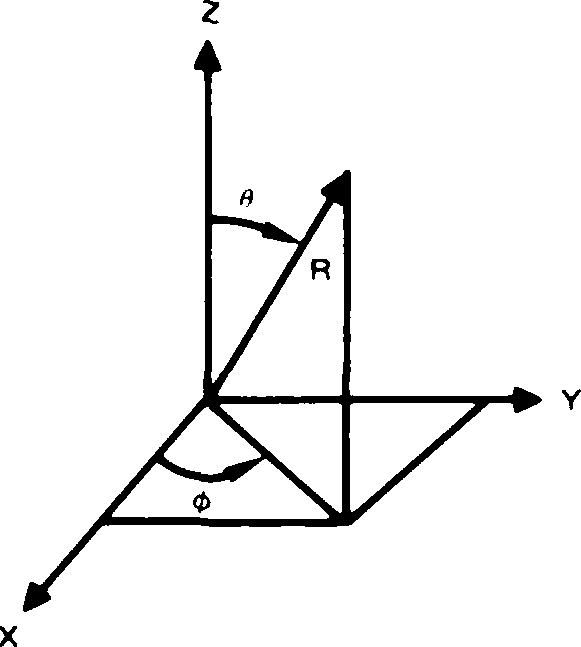
\includegraphics{fig45.eps}}
\caption{Coordinate system for far field pattern}
\label{fig45}
\end{figure}

\subsection{Compute Near Fields}
The \verb+N+ option on the MININEC menu is used to specify the location
of points for calculation of the near electric and magnetic fields. If
the currents have not already been computed, they will be computed
before you can proceed. You must choose electric or magnectic fields.
Then you will be prompted for the field location in cartesian
coordiantes. You are prompted for the initial coordinate, the increment
and the number of steps for each of the principle directions. All
dimensions must be in meters. Next, the radiated power level is
displayed and you are given a chance to change this level. The near
fields will be scaled to the power level you specify. If you specify
zero, the original power level will be used. You will also be prompted
to save the near field data. The field data will be stored in the disk
file you specify. Use \verb+MMPOST+ (see Appendix~\ref{app-B}) or an
editor of your choice to process this data for plotting.

\subsection{Quit}
The \verb+Q+ option on the MININEC menu provides a clean and efficient
termination of the MININEC session.

\clearpage
\bibliography{mininec}
\clearpage

\appendix
\section{A Pre-Processor for MININEC}
\label{sec-appendix-a}
\verb+MNPRE.BAS+ converts NEC input data sets to MININEC geometry
specifications. First prepare an input data file suitable for NEC (see
reference~\cite{r5} for instructions). Then run \verb+MNPRE.BAS+.
\verb+MNPRE.BAS+ will prompt you for a disk file name containing the NEC
data set. It will convert the geometry portion of the NEC data set into
the geometry specifications required by MININEC and write the results
into a binary file named \verb+MININEC.INP+. When you run MININEC, it
will check \verb+MININEC.INP+ for data. If empty, data entry is normal
keyboard entry. If not empty, MININEC will read the data and display the
segmentation data. The MININEC session will then proceed as normal
starting with the question:

\begin{Verbatim}
CHANGE GEOMETRY (Y/N)?
\end{Verbatim}

A source listing of \verb+MNPRE.BAS+ follows:

\section{A Post-Processor MININEC}
\label{app-B}
\verb+MNPOST.BAS+ processes MININEC output data for plotting using the
\verb+GRAPS+ program (See NOSC TD 820, ``GRAPS: Graphical Plotting
System'' by R. T. Laird, July 1985). You may store MININEC currents,
near fields and pattern data in a file of your choice. Election to store
output data in disk files is accomplished during a MININEC session.
\verb+MNPOST.BAS+ will read these files and prompt you for the data to
be plotted. \verb+MNPOST.BAS+ will recognize the type of data and
display it for your convenience. After you have chosen the data for
plotting, the minimum and maximum values are computed and displayed. You
will be prompted to adjust the scale limits or use these values. Then
the data will be written to a file you designate in the format required
by \verb+GRAPS+. A program listing of \verb+MNPOST.BAS+ follows:

\section{MININEC Program Listing}
MININEC Compilation

\newcommand{\slashbreak}{\discretionary{/}{}{/}}
Fastest run times for MININEC3 have been achieved using
87BASIC\slashbreak{}INLINE(TM), MicroWay's BASIC compiler post processor
which generates in-line 8087 code for all floating point expressions.
The following table gives some ideas of the difference in run times for
the matrix fill in the sample problem in NOSC TD 516, Appendix B.

\begin{table}[ht]
\begin{tabular}{lr}
BASICA Interpreter & 4 1/2 hours \\
IBM BASIC Compiler & 22 minutes  \\
87BASIC Compiler   &  8 minutes  \\
87BASIC/INLINE     &  4 minutes  \\
\end{tabular}
\end{table}

87BASIC/INLINE is available from MicroWay, P.O. Box 79, Kingston, Mass.
02364 Phone (617) 746-7341. The current price of the package is two
hundred dollars.

MININEC3.BAS may be run with the BASICA Interpreter, but the maximum
number of pulses must be reduced to 42 with 10 wires. A maximum of 50
wires and 50 pulses may be used with the IBM BASIC Compiler. The other
compilers allow 70 pulses.

A program listing dimensioned for the IBM BASIC Compiler follows:

\end{document}
